%% Vorlage HTBL Hollabrunn Diplomarbeit
%% KOMA Script
\documentclass[12pt,ngerman,a4paper,parskip,twoside,listof=totoc,tikz]{scrartcl}

\usepackage{hhline}     % Tutorial Table border
\usepackage{listings}   % Code Listings
\usepackage{lstlangarm} % ARM ASM
\usepackage{lstlangz80} % Z80 ASM
\usepackage[dvipsnames]{xcolor}

\lstset{
    basicstyle=\ttfamily,
    keywordstyle=\color{ProcessBlue}\ttfamily,
    stringstyle=\color{Red}\ttfamily,
    commentstyle=\color{ForestGreen}\ttfamily,
    morecomment=[l][\color{Thistle}]{\#},
    basicstyle=\footnotesize,
    numbers=left,
    stepnumber=1,
    showstringspaces=false,
    tabsize=1,
    breaklines=true,
    breakatwhitespace=false,
    columns=fullflexible,
}

\usepackage{hyperref}
\usepackage[ngerman]{babel}
\usepackage[german]{fancyref}
\usepackage{subfig}         % Subfigures

\usepackage{htlDT}    % HTBL Diplomarbeitsstyle

\usepackage{todonotes}

%%%%%%%%%%%%%%%%%%%%%%%%%%%%%%%%%%%%%%%%%%%%%%%%%%%%%%%%%%%%%%%%%%%%%%%%%%%%%%%%%%%%%%%%%%%%% General Settings, like Title, Students and supporters
\title{Advanced Microcontroller Training System}
\student{Andreas Mieke}{Software ARM Cortex-M3 Minimalsystem}{5BHEL}{Dipl.-Ing. Josef Reisinger}
\student{Andreas Reischl}{Z80 Minimalsystem}{5AHEL}{Dipl.-Ing. Josef Reisinger}
\student{Kevin Schuh}{Hardware ARM Cortex-M3 Minimalsystem}{5BHEL}{Dipl.-Ing. Josef Reisinger}
\termyear{2017/18}
\class{5xHEL}
\keywords{ST-Link V2\\ULINK/ME\\Cortex-M3\\\gls{cpu}\\Nextion NX4832T035\_011\\JTAG\\SPI\\UART\\I$^2$C\\\gls{Core-Modul}\\\gls{Basisplatine}\\\gls{USB-to-UART}\\Altium\\$\mu$Vision 5\\ARM}
\sthanks{
    Im Vorhinein möchten wir uns herzlichst bei unserem Diplomarbeitsbetreuer Herrn Dipl.-Ing. Josef Reisinger bedanken, der uns stets kompetent beraten hat und uns sein Wissen zur Verfügung stellte.

    Des Weiterem möchten wir uns bei Herrn Dipl.-Ing. Erwin Dobart bedanken, der uns bei technischen Fragen unterstützte. 
    
    Weiters möchten wir uns bei Herrn FOL StR Ing. Manfred Resel bedanken, der uns, solange er noch im Dienst war, bei Softwareproblemen und Hardwarefragen aller Art zur Seite stand. 
    
    Darüber hinaus möchten wir uns bei Herrn Wolfgang Kauer und Herrn Ferdinand Klampfer bedanken, ohne deren Hilfe wir unsere Leiterkarten nicht hätten bestücken können.
    
    Ebenfalls möchten wir Herrn Dipl.-Ing. Wilfried Trollmann bedanken, welcher uns immer an unsere Fristen und Termine erinnerte und uns jederzeit über aktuelle Wettbewerbe informierte.
    
    Außerdem möchten wir uns bei Thomas Fehringer, unseren Laboranten, bedanken, welcher uns mit Bauteilen für unsere Diplomarbeit versorgte.
}

\aufgabenstellung{Aufgabe soll es sein, eine neue Version für das HTL eigene ARM Minimalsystem zu realisieren. Zunächst soll ein Touchscreen-Display zur Ein- und Ausgabe unterstützt werden. Des Weiteren soll eine Arduino-UNO kompatible Schnittstelle zur Verfügung gestellt werden, um Arduino Shields von verschiedenen Herstellern einsetzen zu können. Darüber hinaus soll das neue System verschiedene Funkmodule unterstützen, um damit eine Kommunikation mit anderer Peripherie zu erleichtern. Ein Audiomodul, welches bereits bei einer Diplomarbeit aus dem Jahre 2015/16 entwickelt wurde, soll ebenso unterstützt werden. Zusätzlich soll noch ein Z80 Minimalsystem, welches im Rahmen mehrerer Diplomarbeiten entstanden ist, für den Einsatz im Laborunterricht vervollständigt werden.}

\realisierung{Zuerst sollen die einzelnen Arbeitsaufträge entwickelt und überprüft werden. Anschließend sollen die einzelnen Systemkomponenten zum fertigen System zusammengefügt und in Betrieb genommen werden. Die Funktion und die einzelnen Entwicklungsschritte zum fertigen Prototypen sollen anschließend durch eine umfangreiche Dokumentation und eine Bedienungsanleitung vervollständigt werden.}

\ergebnisse{Es wurden funktionsfähige Prototypen aller Leiterkarten gefertigt. Darüber hinaus wurde eine Testsoftware zur Überprüfung der Prototypen geschrieben.}

\grafikname{Gesamtsystem}
\grafikinhalt{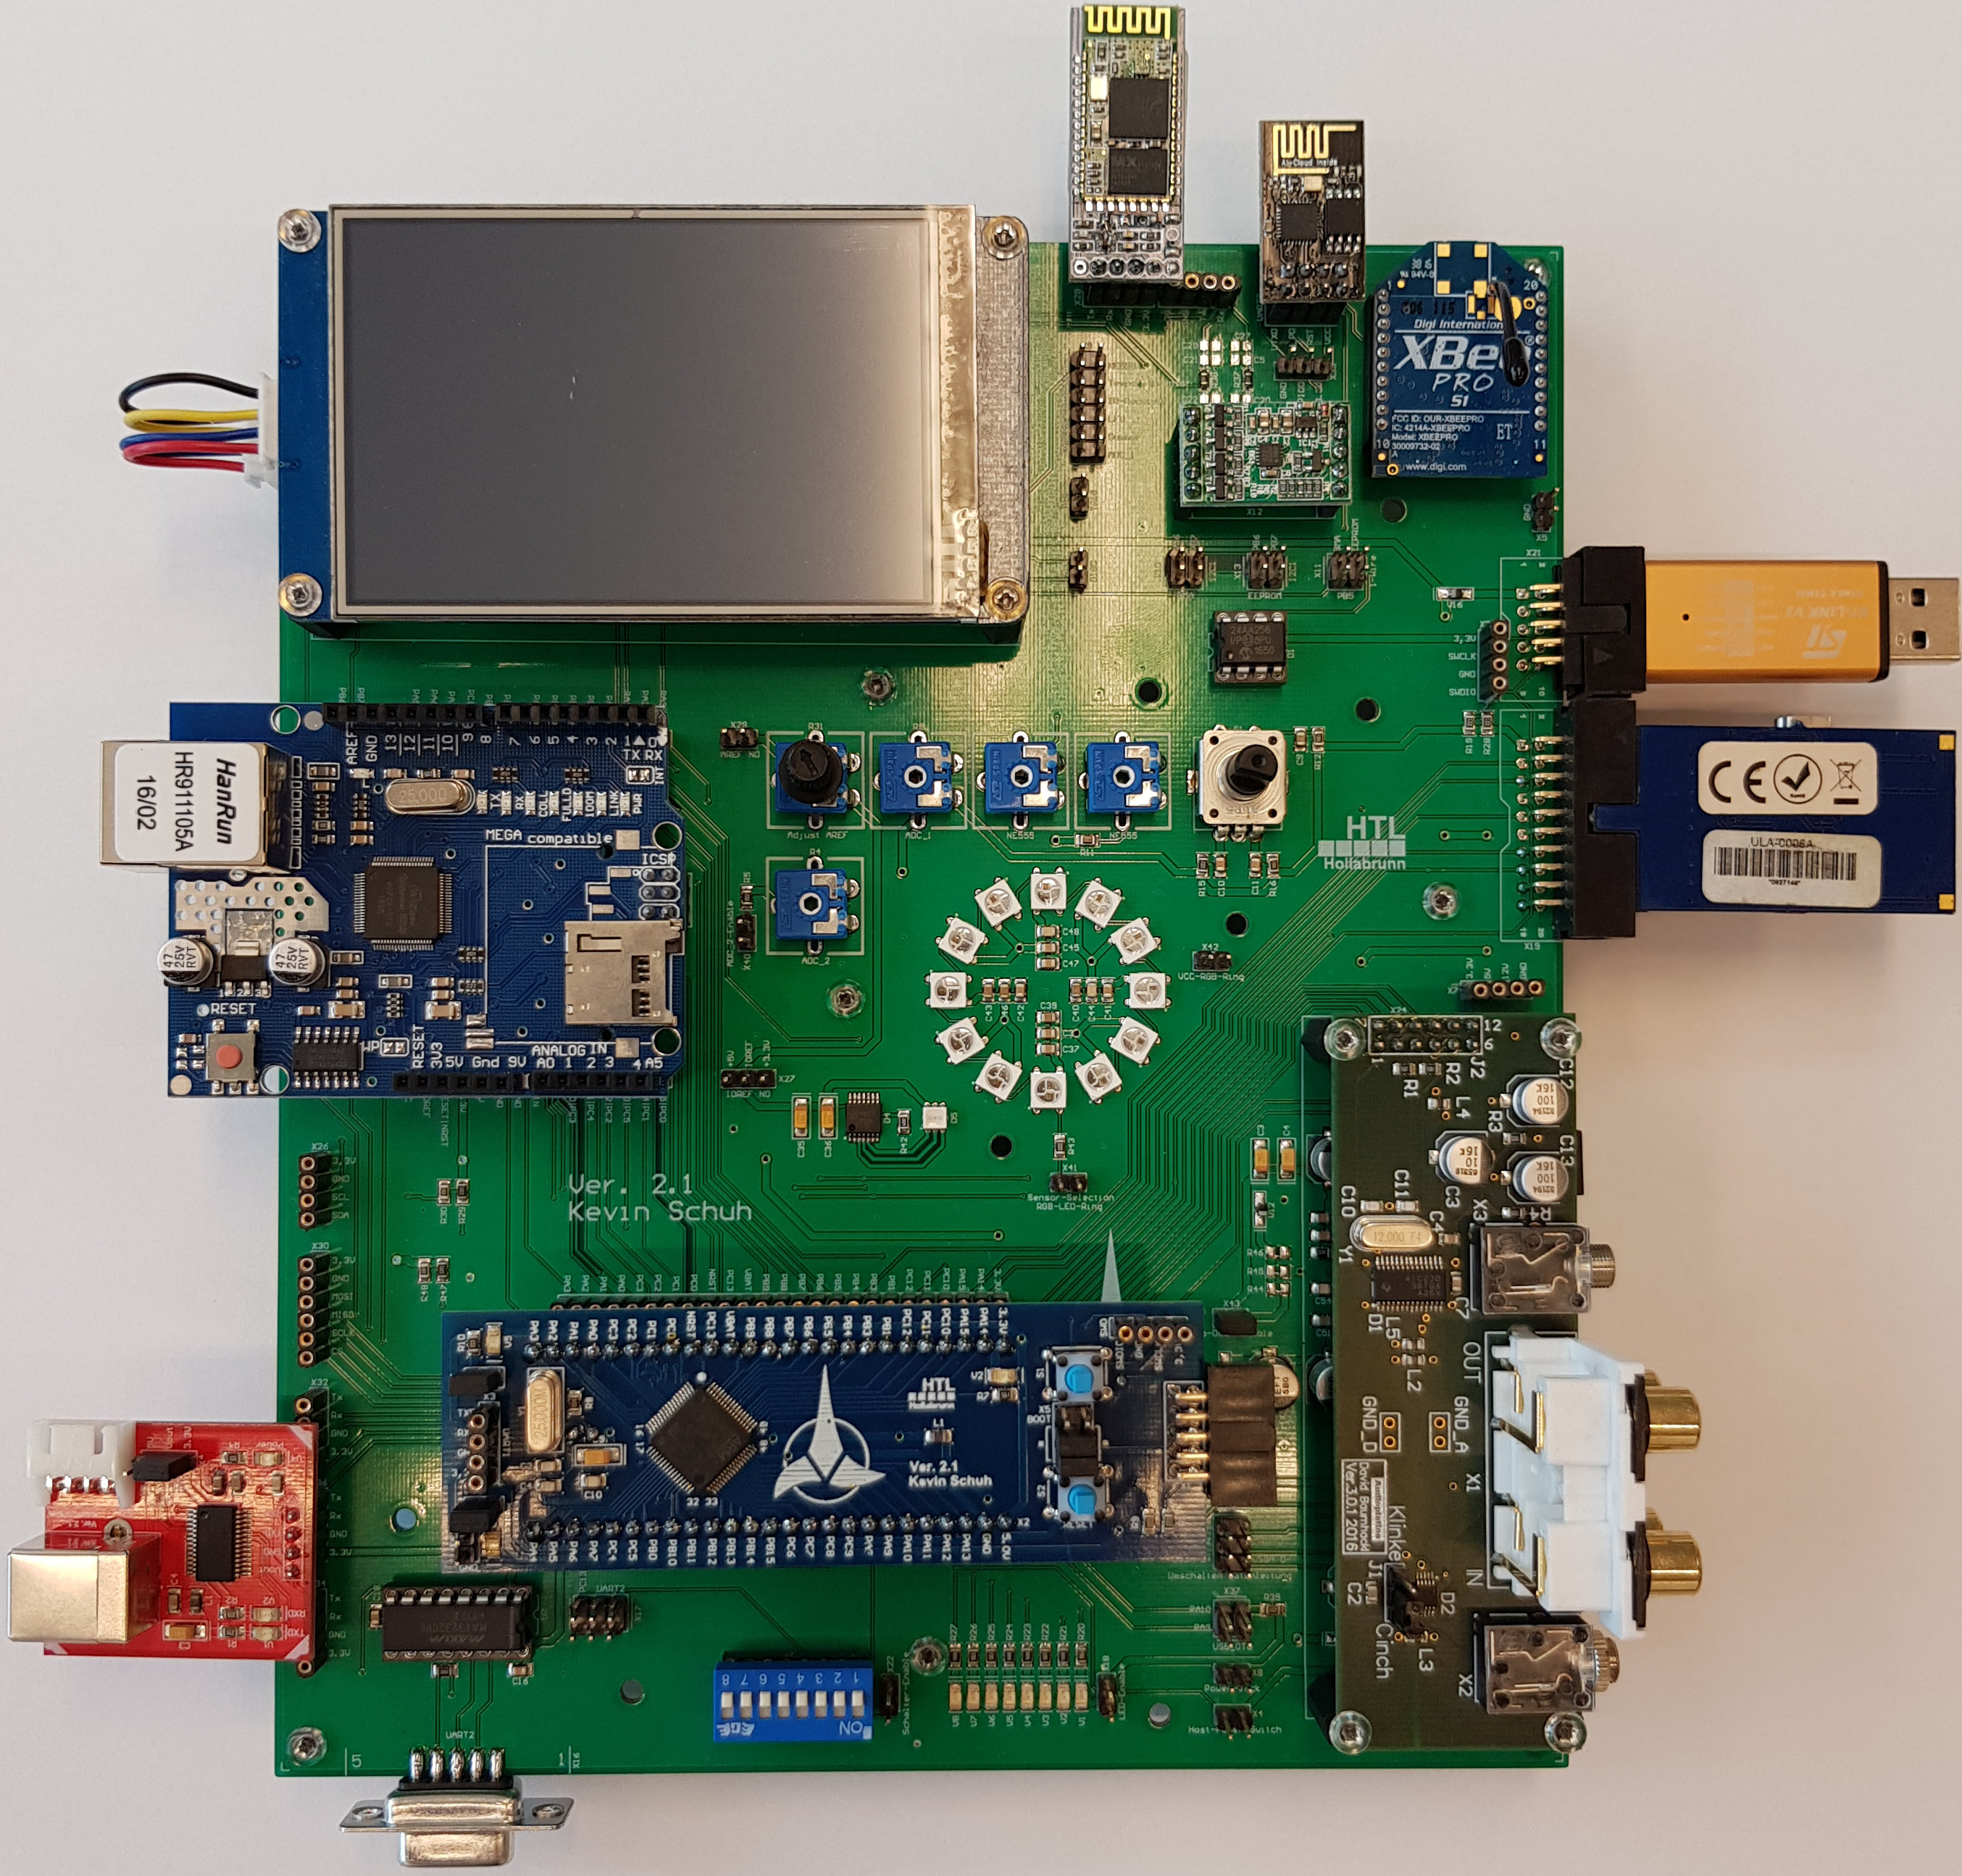
\includegraphics[width=\textwidth]{Allgemein/img/Gesamtsystem}}

\wettbewerbe{Jugend Innovativ\\Technik fürs Leben-Preis}



\tasks{The task should be to realize a new version for the HTL (secondary technical college) own ARM minimal system. At first, a touchscreen display for input and output should be supported. Furthermore, an Arduino-UNO compatible interface should make it possible to use Arduino shields from different manufacturers.  In addition, the new system should support various wireless modules to facilitate communication with other peripherals. An audio module, which was already developed in a diploma thesis from the year 2015/16, should also be supported. In addition, a Z80 minimal system, which was created in the context of several diploma theses, should be finalised for the use in laboratory lessons.}

\realisation{At first, the individual work orders should be developed and checked. Subsequently, the individual system components were to be assembled into the finished system and put into operation. The function and the individual development steps for the finished prototype should be completed with a documentation and a user manual.}

\results{Working prototypes of all printed circuit boards have been developed. Moreover, a test software to prove the functionality of the prototype has been written.}

\graphname{System overview}
\graphcontent{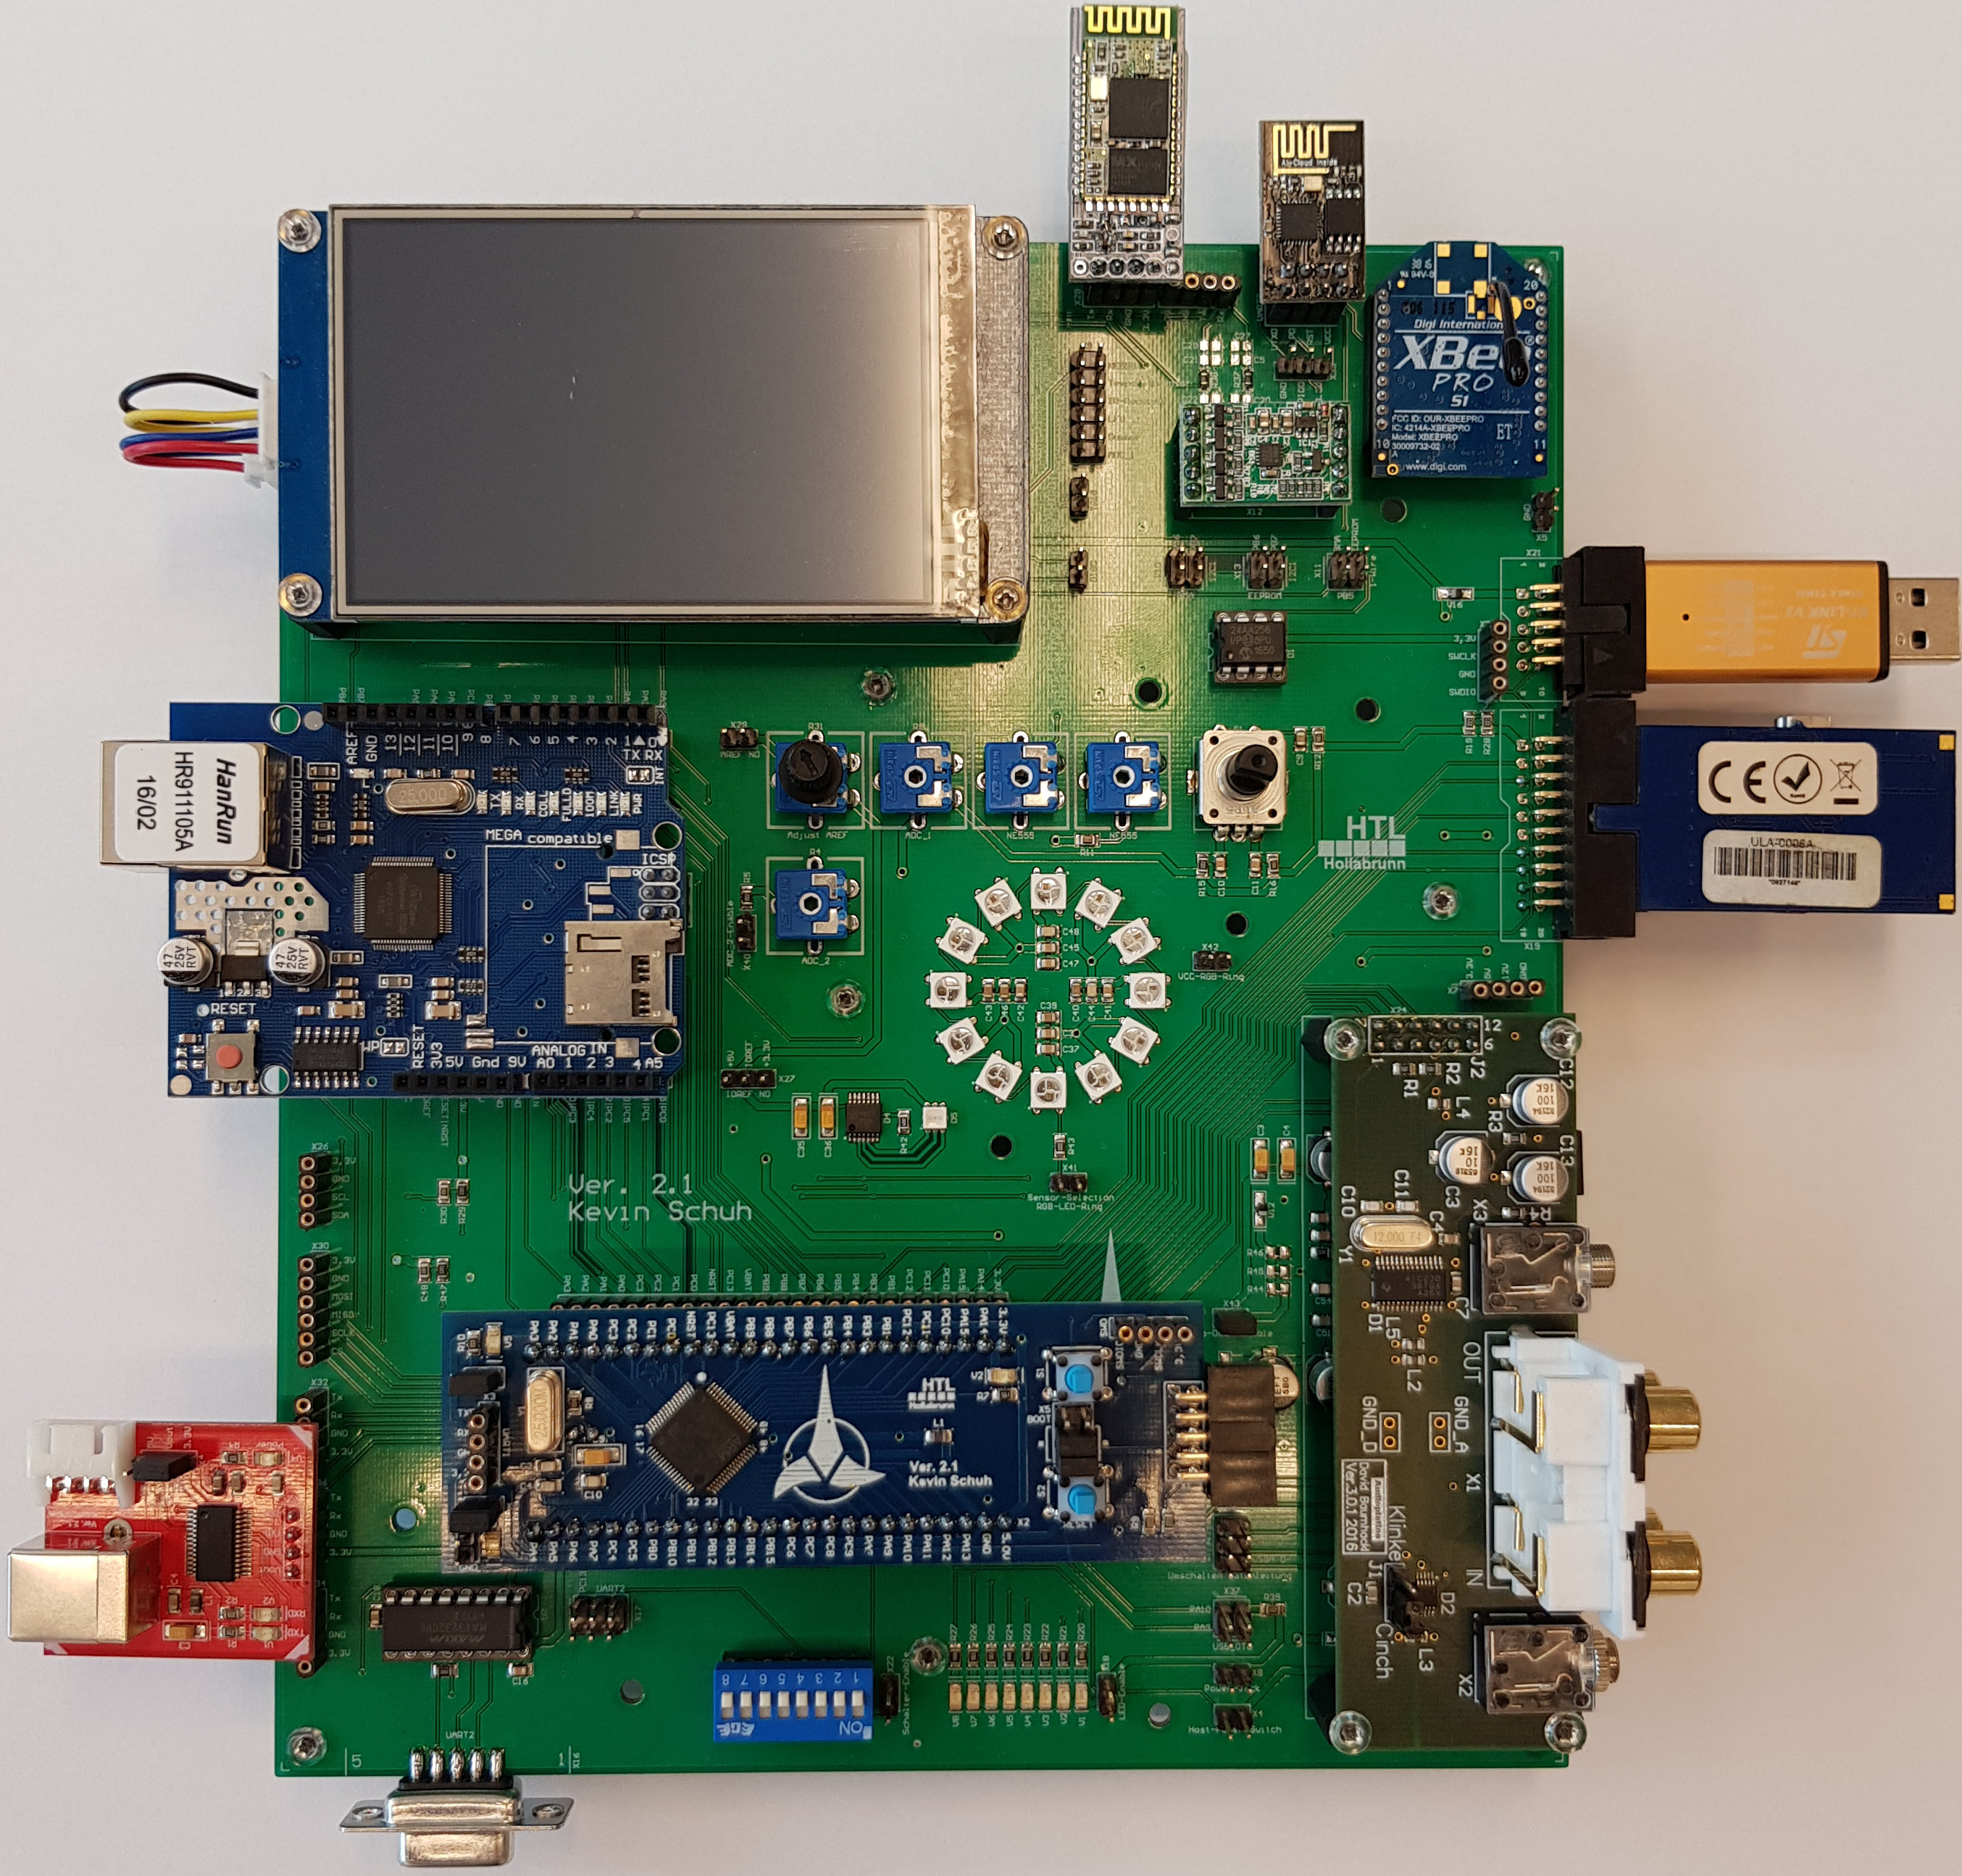
\includegraphics[width=\textwidth]{Allgemein/img/Gesamtsystem}}

\competitions{Jugend Innovativ\\Technik fürs Leben-Preis}

%%%%%%%%%%%%%%%%%%%%%%%%%%%%%%%%%%%%%%%%%%%%%%%%%%%%%%%%%%%%%%%%%%%%%%%%%%%%%%%%%%%%%%%%%%%%% Bibliography
\usepackage[backend=bibtex, style=ieee, citestyle=ieee, hyperref=true]{biblatex}
\makeatletter
\def\blx@maxline{77}
\makeatother

\usepackage{xpatch}
\makeatletter 
\xpatchcmd\blx@head@bibliography{\markboth}{\@mkboth}{}{\undefined} 
\makeatother

\addbibresource{literatur.bib}

%%%%%%%%%%%%%%%%%%%%%%%%%%%%%%%%%%%%%%%%%%%%%%%%%%%%%%%%%%%%%%%%%%%%%%%%%%%%%%%%%%%%%%%%%%%%% Gloassaries
\usepackage[nomain,acronym,toc,section]{glossaries}
\makeglossaries
\makeindex

\usepackage{xparse}
\DeclareDocumentCommand{\newdualentry}{ O{} O{} m m m m } {
  \newglossaryentry{gls-#3}{name={#5},text={#5\glsadd{#3}},
    description={#6},#1
  }
  \makeglossaries
  \newacronym[see={[Siehe:]{gls-#3}},#2]{#3}{#4}{#5\glsadd{gls-#3}}
}
% Usage: \newdualentry{ref}{short}{long}{description}

%%%%%%%%%%%%%%%%%%%%%%%%%%%%%%%%%%%%%%%%%%%%%%%%%% Acronyms
\newdualentry{IDE}{IDE}{integrierte Entwicklungsumgebung}{ist Deutsch für \enquote{Integrated Development Environment} und beschreibt eine Sammlung von Programmen (Editor, Compiler, Linker, Loader, Debugger), welche zum programmieren verwendet wird \cite{wiki:IDE}}

\newdualentry{ARM}{ARM}{ARM Limited}{früher: Advanced RISC Machines Ltd. ist ein zur japanischen Firma Softbank gehörender Hersteller von IP (Intellectual property) Software im Bereich Mikroprozessoren. Die gleichnamige Mikroprozessorarchitektur, ARM, ist zur Zeit weltweit am weitesten verbreitet \cite{wiki:ARM} \cite{techradar:ARM}}

\newdualentry{CMSIS}{CMSIS}{Cortex Microcontroller Software Interface Standard}{ist ein von \gls{ARM} erstellter Standard, welcher das Verwenden von Software zwischen verschiedenen Cortex-Prozessoren verschiedener Chip-Hersteller ohne große Anpassungen ermöglichen soll. Hierfür stellt \gls{ARM} einige Definitionen -- wie zum Beispiel CORE, RTOS, DSP, \dots{} -- zur Verfügung, welche von den Chip-Herstellern implementiert werden, diese stellen dann CMSIS-Packs zur Verfügung, welche in Softwareprojekte eingebunden werden können. Siehe: \cite{arm:CMSIS}}

\newdualentry{SWD}{SWD}{Single Wire Debug}{ist ein Subset von \gls{JTAG}, welches mit weniger Portleitungen auskommt}

\newdualentry{JTAG}{JTAG}{Joint Test Action Group}{ist ein Synonym für den IEEE Standard 1149.1, welcher eine Methodik zum \gls{Debugging} von Hardware auf Leiterplatten beschreibt. Siehe: \cite{ieee:1149-1}}

\newdualentry{STDLib}{STDLib}{HTL Standard Library}{ist eine Library für den Cortex-M3, welche HTL-spezifische Funktionen, vor allem im Bereich I/O enthält}

\newdualentry{Keil}{Keil}{Keil Elektronik GmbH}{war eine deutsche Firma (Anfangs: GbR), gegründet 1982 von Günther und Reinhard Keil. Das Hauptaufgabengebiet lag bei der Entwicklung von Evaluation Boards und der $\mu$Vision \gls{IDE}. Keil wurde 2005 von \gls{ARM} aufgekauft. Siehe: \cite{wiki:Keil} \cite{techdesignforums:ARM}}

\newdualentry{XML}{XML}{Extensible Markup Language}{ist eine Auszeichnungssprache, welche zur Abspeicherung von strukturierten Daten verwendet wird}

\newdualentry{MMI}{MMI}{Mensch-Maschine-Interface}{ist ein Interface (z.B.: Display, Tastatur) um die Kommunikation von einem Menschen mit einer Maschine zu ermöglichen}

\newdualentry{DSV}{DSV}{Digitale Signalverarbeitung}{ist eine Methodik um ursprünglich analoge Bauelemente wie Filter oder Oszillatoren digital zu realisieren, Siehe auch: \gls{DSP}}

\newdualentry{GUI}{GUI}{Graphical User Interface}{englisch für \enquote{grafische Benutzeroberfläche}. Teil des \gls{MMI}}

\newdualentry{STM}{STM}{STMicroelectronics N.V.}{ist ein europäischer Halbleiterhersteller mit Sitz in den Niederlanden. Siehe: \cite{wiki:STM}}

\newdualentry{RTC}{RTC}{Real Time Clock}{zu deutsch: Echtzeituhr, ist eine Uhr, welche durch die hohe Präzision dafür ausgelegt ist Zeitnahmeaufgaben zu erledigen\todo{Stimmt das so??}}

\newdualentry{ADC}{ADC}{Analog-Digital-Converter}{zu deutsch: Analog-Digital-Wandler, ist ein Bauteil, welches Wert- und Zeitkontinuirliche Signale Abtastet und Quantisiert um sie digital weiter verarbeiten zu können}

\newdualentry{DSP}{DSP}{Digital Signal Processor}{zu deutsch: Digitaler Signalprozessor, wird verwendet um digitalisierte Signale weiterzuverarbeiten}

\newdualentry{DAC}{DAC}{Digital-Analog-Converter}{zu deutsch: Digital-Analog-Wandler, ist ein Bauteil, welches Wert- und Zeitdiskrete Signale analog ausgibt}

\newdualentry{SNR}{SNR}{Signal-Noise-Ratio}{zu deutsch: Signal-Rausch-Abstand, gibt an, wie viele \deci\bel zwischen Signal und Rauschen liegen}

\newdualentry{MSb}{MSB}{Most Significant Bit}{zu deutsch: relevantestes Bit, das Bit mit dem höchsten Wert}

\newdualentry{LSb}{LSB}{Least Significant Bit}{zu deutsch: irrelevantestes Bit, das Bit mit dem kleinsten Wert}

\newdualentry{MSB}{MSB}{Most Significant Byte}{zu deutsch: relevantestes Byte, das Byte mit dem höchsten Wert}

\newdualentry{LSB}{LSB}{Least Significant Byte}{zu deutsch: irrelevantestes Byte, das Byte mit dem kleinsten Wert}

%%%%%%%%%%%%%%%%%%%%%%%%%%%%%%%%%%%%%%%%%%%%%%%%%% Glossary
\newglossaryentry{Debugging}{
  name={Debugging},
  description={oder \enquote{Debuggen} beschreibt das finden und entfernen von Bugs (engl. für Käfer, hier: Programmfehler) mit Hilfe eines Debuggers. Siehe: \cite{wiki:Debugger}}
}

\newglossaryentry{Minimalsystem}{
  name={Minimalsystem},
  description={beschreibt das im Unterricht üblicherweise verwendete -- aber auch erweiterbare -- Microcontroller System}
}

\newglossaryentry{Core-Modul}{
  name={Core-Modul},
  description={ist die Baugruppe, auf welcher der Cortex-M3 Prozessor sitzt und Teil des neuen \gls{Minimalsystem}s}
}

\newglossaryentry{Basisplatine}{
  name={Basisplatine},
  description={ist die Baugruppe, auf welche das \gls{Core-Modul} gesteckt wird. Sie bietet Schalter, LEDs, Sensoren und ein Arduino Shield Interface. Zusammen mit dem \gls{Core-Modul} komplettiert sie das \gls{Minimalsystem}}
}

\newglossaryentry{USB-to-UART}{
  name={USB-to-UART},
  description={ist die Baugruppe, welche ein UART Gerät über USB emuliert. Es verwendet hierfür einen FTDI-Chip und ist Teil des neuen \gls{Minimalsystem}s}
}

\newglossaryentry{C}{
  name={C},
  description={ist eine Programmiersprache, welche sowohl zur System- als auch zur Anwendungsprogrammierung eingesetzt wird. C ist eine der am weitesten verbreiteten Programmiersprachen weltweit und wurde in den 1970er-Jahren von Dennis Ritchie erfunden. Siehe: \cite{wiki:C}}
}

\newglossaryentry{C++}{
  name={C++},
  description={ist eine objektorientierte Erweiterung zu \gls{C}. C++ wurde 1979 von Bjarne Stroustrup entwickelt. Siehe: \cite{wiki:C++}}
}

\newglossaryentry{ZIP}{
  name={ZIP},
  description={ist ein weit verbreitetes Dateiformat, welches zur Archivierung und Kompression von Dateien und Ordnern verwendet wird. Der Name leitet sich aus dem englischen Wort \enquote{zipper} (Reißverschluss) ab}
}

\newglossaryentry{Semantic Versioning}{
  name={Semantic Versioning},
  description={beschreibt eine Art der Versionierung von Software, welche aus 3 einzelnen Versionsnummern im Format A.B.C besteht, C steht hierbei für Patches (Bugfixes, keine neue Funktionalität), B für Minor Versions (neue Funktionalität, aber weiterhin kompatibel zur Vorgängerversion) und A, was Major Versions (inkompatibel zu älteren Versionen) darstellt}
}

\newglossaryentry{cpu}{
  name={STM32F107RCT(6)},
  description={ist der in dieser Diplomarbeit verwendete Microcontroller}
}

%%%%%%%%%%%%%%%%%%%%%%%%%%%%%%%%%%%%%%%%%%%%%%%%%%%%%%%%%%%%%%%%%%%%%%%%%%%%%%%%%%%%%%%%%%%%% Begin Document
\begin{document}
\newcommand*{\IIC}{I$^2$C}
\newcommand*{\IIS}{I$^2$S}
\newcommand*{\uVision}{$\mu$Vision}
%%%%%%%%%%%%%%%%%%%%%%%%%%%%%%%%%%%%%%%%%%%%%%%%%%%%%%%%%%%%%%%%%%%%%%%%%%%%%%%%%%%%%%%%%%%%% Titlepage, DA database and TOC
\maketitle{}
\makedadb{pdfs/DADB}{pdfs/DADBErklarung}
\maketoc

%%%%%%%%%%%%%%%%%%%%%%%%%%%%%%%%%%%%%%%%%%%%%%%%%%%%%%%%%%%%%%%%%%%%%%%%%%%%%%%%%%%%%%%%%%%%% First real page
\pageauthor{Schuh}
\section{Allgemeines}
\label{sec:allgemeines}

\subsection{Entstehungsgeschichte}
\label{sec:entstehungsgeschichte}

Seit mehreren Jahren wird in der HTBL-Hollabrunn, ein \gls{ARM} Cortex-M3 \gls{Minimalsystem}, für die Ausbildung unserer Schüler, im Bereich \enquote{embedded Systems} eingesetzt.

Wie schon im Abstract beschrieben geht es bei dem neuen System darum, sich neuen Technologien und Anwenderszenarien zu öffnen beziehungsweise schnelles Prototyping (Rapid Protoyping) zu ermöglichen. Mit Hilfe des Nextion-Touchscreen-Displays wird ein modernes \gls{MMI} bereitgestellt, um Anwendungen leichter und interaktiv bedienbar zu machen. Das Audio-Interface ermöglicht es, Anwendungen für digitale Signalverarbeitung (z.B. digitale Filter) zu realisieren. Das Arduino-Interface ermöglicht es, verschiedenste Arduino-Shields für den Unterricht einzusetzen. Diese Schnittstellen, sowie die Schnittstellen für WLAN, Bluetooth und Funkmodule ermöglichen es auf schnelle Art und Weise Konzepte für Diplomarbeiten zu evaluieren.

\subsection{Anwendungsszenarien}
\label{sec:anwendungsszenarien}

Das gesamte \gls{ARM}-\gls{Minimalsystem} soll dazu beitragen, mit Hilfe einer Vielzahl an Schnittstellen, hardwarenahe Programmierung zu erlernen, sowie das Bauen und Testen von Prototypen zu erleichtern. Weiters kann aufgrund, des auf der \gls{Basisplatine} vorhandenen Arduino-Sockels eine Kompatibilität zu allen Arduino-Shields erreicht werden, welche nun über das \gls{Core-Modul} angesteuert werden können.

Das Hauptaugenmerk wurde jedoch auf folgende Anwendungen gelegt:

\begin{itemize}
    \item \gls{DSV}
    \item Kommunikation mit diversen Schnittstellen (\IIC{}, SPI, UART, 1-Wire, \dots{})
    \item Hardwarekompatibilität zu Arduino-Shields
    \item \gls{GUI}
\end{itemize}

\fig{anwendung-gpio}{Anwendungsszenario: GPIO}{Anwendungsszenario: GPIO}{0.75\textwidth}{Allgemein/img/Anw/io-gpio}
\fig{anwendung-uart}{Anwendungsszenario: UART}{Anwendungsszenario: UART}{0.75\textwidth}{Allgemein/img/Anw/io-uart}
\fig{anwendung-periph}{Anwendungsszenario: Serielle Kommunikation}{Anwendungsszenario: Serielle Kommunikation}{0.5\textwidth}{Allgemein/img/Anw/io-periph}
\fig{anwendung-timerinterrupt}{Anwendungsszenario: Timer/Interrupt}{Anwendungsszenario: Timer/interrupt}{0.75\textwidth}{Allgemein/img/Anw/capture-compare}
\fig{anwendung-audio}{Anwendungsszenario: Audioverarbeitung}{Anwendungsszenario: Audioverarbeitung}{0.75\textwidth}{Allgemein/img/Anw/audio}
\fig{anwendung-ethernet}{Anwendungsszenario: Webanwendung}{Anwendungsszenario: Webanwendung}{0.75\textwidth}{Allgemein/img/Anw/ethernet}
\fig{anwendung-bluetooth}{Anwendungsszenario: Bluetooth}{Anwendungsszenario: Bluetooth}{0.75\textwidth}{Allgemein/img/Anw/bluetooth}
\fig{anwendung-usbhid}{Anwendungsszenario: USB HID}{Anwendungsszenario: USB HID}{0.75\textwidth}{Allgemein/img/Anw/usb-hid}
\fig{anwendung-usbhost}{Anwendungsszenario: USB Host}{Anwendungsszenario: USB Host}{0.75\textwidth}{Allgemein/img/Anw/usb-host}

\pageauthor{Mieke}
\section{Theorie}
\label{sec:theorie}
\subsection{Versionierung}
Das Kapitel Versionierung teilt sich in zwei große Teile auf, Semantic Versioning, was die Vergabe der Versionsnummer an sich behandelt und Git, was im generellen Workflow zur Versionskontrolle benutzt wurde.

\subsubsection{Semantic Versioning}
Semantic Versioning, oder auch semantische Versionierung bezeichnet ein Verfahren zur Vergabe von Versionsnummern welches sich als sehr praktisch zum Versionieren von Softwarekomponenten herausgestellt hat. Heute benutzen sehr viele große Softwareprojekte, vor allem im Open Source Bereich, Semantic Versioning für die Versionierung von Releases.

Bei Semantic Versioning setzt sich die Versionsnummer aus drei Hauptgruppen welche aus Ziffern bestehen und durch einen Punkt getrennt sind zusammen. Jede dieser Gruppen hat eine festgelegte Bedeutung, von links nach rechts heißen die Gruppen \enquote{Major}, \enquote{Minor} und \enquote{Patch}.

Ein Produkt mit der Versionsnummer \textbf{2.5.15} hat also die Major-Version \textbf{2}, Minor-Version \textbf{5} und Patch-Level \textbf{15}.

Will man nun eine neue Version der Software (oder des Produkts) veröffentlichen, so muss man, je nach Änderung, die Versionsnummer erhöhen. Hierbei wird meist nach \fref{tab:versionierung} vorgegangen.

\tab{versionierung}{Semantic Versioning Zifferngruppen}{Zifferngruppen}{|c|p{10cm}|}{
    \hline
    \textbf{Gruppe} & \textbf{Bedeutung}\\
    \hline
    Patch & wird erhöht wenn Fehler in der Software ausgebessert werden, jedoch keine neuen Funktionen hinzugefügt werden. Binäre Bibliotheken bleiben untereinander komplett kompatibel.\\
    \hline
    Minor & wird erhöht wenn neue Funktinen hinzugefügt werden, nebenbei können auch Fehler ausgebessert werden, ohne eine Erhöhung des Patch Levels zu erfordern. Binäre Bibliotheken sind abwärtskompatibel, das heißt Bibliotheken mit Version \textbf{2.15.6} können anstatt Version \textbf{2.10.0} verwendet werden. Umgekehrt ist das aber nur so lange möglich, so lange mein keine erweiterten Funktionen aus der Bibliothek mit der höheren Minor-Version verwendet.\\
    \hline
    Major & wird erhöht wenn einerseits neue Funktionen hinzugefügt werden, allerdings gleichzeit auch alte gelöscht oder sonst irgendwie inkompatibel gemacht (Umbennenung, Änderung der Übergabeparameter) werden. Binäre Bibliotheken sind, bis auf wenige Ausnahmen, normalerweise nicht kompatibel.\\
    \hline
}

Für die Softwareprodukte, welche im Rahmen dieser Diplomarbeit entstanden sind, wurde Semantic Versioning angewendet, um zukünftigen Nutzern oder Bearbeitern ein solides Fundament in Sachen Kompatibilität zu gewähren.

\subsubsection{Git}
Git ist ein dezentrales Versionskontrollsystem, welches erlaubt Zeitpunkte in der Softwareentwicklung (mit Kommentaren versehen) festzuhalten, zwischen diesen zu springen und Teile von oder komplette Änderungen rückgängig zu machen, wenn dies nötig sein sollte. Git legt hierbei für jedes Projekt ein dezentrales Repository an, welches, je nach belieben auch quasi-zentral auf einem Server liegen kann. In einem Repository kann man dann entweder alleine, oder zusammen mit einer oder mehreren Personen am selben Projekt arbeiten. Git übernimmt dabei die Versionskontrolle und in den meisten Fällen auch erfolgreich die Konflktlösung.

\subsubsubsection{Repository anlegen}
Um die Arbeit an einem Projekt beginnen zu können, muss erstmal ein leeres Git-Repository erstellt werden, dies geschieht mit dem Befehl \texttt{git init}. Dieser Befehl legt im Verzeichnis, in dem man sich gerade befindet, einen \texttt{.git}-Ordner an, in welchem Git seine internen Daten speichert.

\subsubsubsection{Der erste Commit}
Nun, da ein Repository angelgt ist, kann die eigentliche Arbeit am Projekt beginnen, so wie man das gewöhnt ist. Wenn man nun vorzeigbare Ergebnisse hat, oder seinen Fortschritt vor größeren Änderungen sichern will, muss man einen Commit erstellen, dieser bildet dann den aktuellen Zustand des Projekts (mit Dateiberechtigungen) und kompletten Inhalt ab. Wenn man später zu diesem Zustand zurückkehren will, kann man einfach auf den Commit zurückkehren. Weiters speichert Git die Änderungen von einem zum nächsten Commit in einem Diff-Format, was bedeutet, dass nicht immer die ganze Datei, sondern nur die Änderungen zur letzten Version, gespeichert werden. Dies ist für ASCII-Dateien (wie zum Beispiel auch Source-Code) sehr effizient, da nicht geänderte Zeilen nicht immer abgespeichert werden müssen.

Um nun die gemachten Änderungen in den Staging-Bereich hinzuzufügen führt man nun entweder \texttt{git add -A} (für alle Dateien und Verzeichnisse) oder \texttt{git add <file.name>} für genau eine (oder mehrere angegebene) Datei(en). Nun können entweder noch weitere Dateien hinzugefügt, Dateien wieder aus dem Staging-Bereich entfernt (\texttt{git reset HEAD <file.name>}) oder ein Commit erstellt werden. Letzteres wird mit dem Befehl \texttt{git commit} gemacht, dieser öffnet den Standard-Texteditor, in welchem man eine Nachricht (meistens die Änderungen, die man gemacht hat) eingibt. Wird der Befehl mit dem Flag \texttt{-m "Nachricht"} ausgeführt, so geht kein Editor auf und der Commit wird direkt mit der angegebenen Nachricht erstellt.

\subsubsubsection{Zurück zu einer alten Version}
Wenn man nun feststellt, dass das, was man programmiert hat nicht zielführend ist oder sich gar negativ auf das Projekt ausgewirkt hat, kann man relativ einfach wieder auf eine funktionierende Version zurück kehren. Hierzu führt man zuerst \texttt{git log} aus, was dann die IDs aller Commits und die erste Zeile der Commit-Nachricht anzeigt, hier sucht man sich nun die ID heraus, zu der man zurück kehren will, und gibt diese bei \texttt{git checkout <commitid>} ein. Nun stellt Git wieder die Version her, wie sie zum Zeitpunkt des Commits existierte.

\subsection{Nextion Editor}

\subsection{\LaTeX{}}
Zum setzen der Dokumentation und anderer aus dieser Diplomarbeit resultierenden Dokument wurde \LaTeX{} verwendet. Die Verwendung von \LaTeX{} bietet im Gegensatz zu anderer Software einige Vorteile, wie zum Beispiel die einfacher Literaturverwaltung mittels BiB\LaTeX{} und das einfache erstellen von Tabellen und ähnlichem direkt in einem handelsüblichen Texteditor. Des weiteren ist es möglich ganze Dokumente in quasi unendlich kleine Teile aufzuteilen, sodass mehrere Leute parallel an einem Gesamtdokument arbeiten können.

\newpage
\pageauthor{Schuh}
\subsection{Systemaufbau}
\label{sec:systemaufbau}

Das neue \gls{ARM}-\gls{Minimalsystem} kann prinzipiell in vier voneinander getrennten Platinen unterteilt werden. Diese Module wären die \gls{Basisplatine}, das \gls{Core-Modul}, der \gls{USB-to-UART} Adapter und der Audioadapter. Jedes dieser Module erfüllt einen bestimmten Zweck, welcher schlussendlich zum Gesamtsystem beträgt.

\fig{gesamtsystem}{Gesamtsystem}{Gesamtsystem}{\textwidth}{Allgemein/img/Gesamtsystem}


\clearpage
\pageauthor{Schuh}
\section{Core-Modul}
\label{sec:coremodul}

\fig{core-modul}{Core-Modul}{\gls{Core-Modul}}{\textwidth}{Schuh/Pictures/coremodul}

\subsection{Allgemeines}
\label{sec:coremodul-allgemeines}

Das \gls{Core-Modul} ist das Herzstück des gesamten \gls{ARM}-\gls{Minimalsystem}s, denn auf diesem befindet sich der Prozessor und alle Komponenten welche für den ordnungsmäßigen Betrieb erforderlich sind. Die einzelnen Port-Pins des Prozessors sind entweder direkt auf dem \gls{Core-Modul} verwendet oder über externe Anschlüsse nach außen geführt. Weiters verfügt das \gls{Core-Modul} über alle nötigen Programmierschnittstellen um unabhängig von der \gls{Basisplatine} oder anderen Programmierplatinen programmiert und verwendet werden zu können. Darüber hinaus kann mit der auf dem \gls{Core-Modul} befindlichen UART-Schnittstelle eine direkte Kommunikation mit anderen Modulen oder einem Terminal aufgebaut werden.

\subsection{Schnittstellen}
\label{sec:coremodul-schnittstellen}

Das \gls{Core-Modul} verfügt über die in \fref{tab:coremodul-schnittstellen} angegebenen Schnittstellen, welche wie in \fref{fig:coremodul-plan} zu sehen platziert sind.

\tab{coremodul-schnittstellen}{Schnittstellen des Core-Moduls}{Schnittstellen des \gls{Core-Modul}s}{|c|p{10cm}|}{
    \hline
    \textbf{Schnittstelle} & \textbf{Funktion}\\
    \hline
    USART 1 & Universal Synchronous/Asynchronous Receiver/Transmitter, Datenübertragung\\
    \hline
    SWD & \gls{SWD}, Programmierung\\
    \hline
    ST-Link V2 & Programmierung auf Basis von \gls{SWD}\\
    \hline
    50 poliger Header & Ausführung der Port-Pins auf die \gls{Basisplatine}\\
    \hline
}

\fig{coremodul-plan}{Übersichtsplan des Core-Moduls}{Übersichtsplan des \gls{Core-Modul}s}{0.75\textwidth}{Schuh/Pictures/Core}

\subsection{Prozessor}
\label{sec:coremodul-prozessor}

Als Prozessor für das \gls{Core-Modul} wurde der \gls{cpu} von der Firma \gls{STM} verwendet. Die Key-Features werden in \fref{fig:coremodul-features} zusammengefasst.

\fig{coremodul-features}{Features des Prozessors}{Features des Prozessors \cite{stm:stm32f107rc-web}}{\textwidth}{Schuh/Pictures/Features}

\subsubsection{Blockschaltbild}
\fig{coremodul-cpubsb}{Blockschaltbild des Prozessors}{Blockschaltbild des Prozessors \cite{stm:stm32f107rc}}{0.8\textwidth}{Schuh/Pictures/BSB}

\subsubsection{Pinning}
\fig{coremodul-cpupinning}{Pinning des Prozessors}{Pinning des Prozessors \cite{stm:stm32f107rc}}{0.8\textwidth}{Schuh/Pictures/Pinning}

\subsubsection{Abmessungen}
\fig{coremodul-cpumeasure}{Abmessungen des Prozessors}{Abmessungen des Prozessors \cite{stm:stm32f107rc}}{0.8\textwidth}{Schuh/Pictures/MeasureGraphic}
\tabpdf{coremodul-cpumeasure}{Abmessungen des Prozessors}{Abmessungen des Prozessors \cite{stm:stm32f107rc}}{0.8\textwidth}{Schuh/Pictures/MeasureTable}

\subsubsection{Pinbelegung}
\begin{table}[htb]
    \centering
    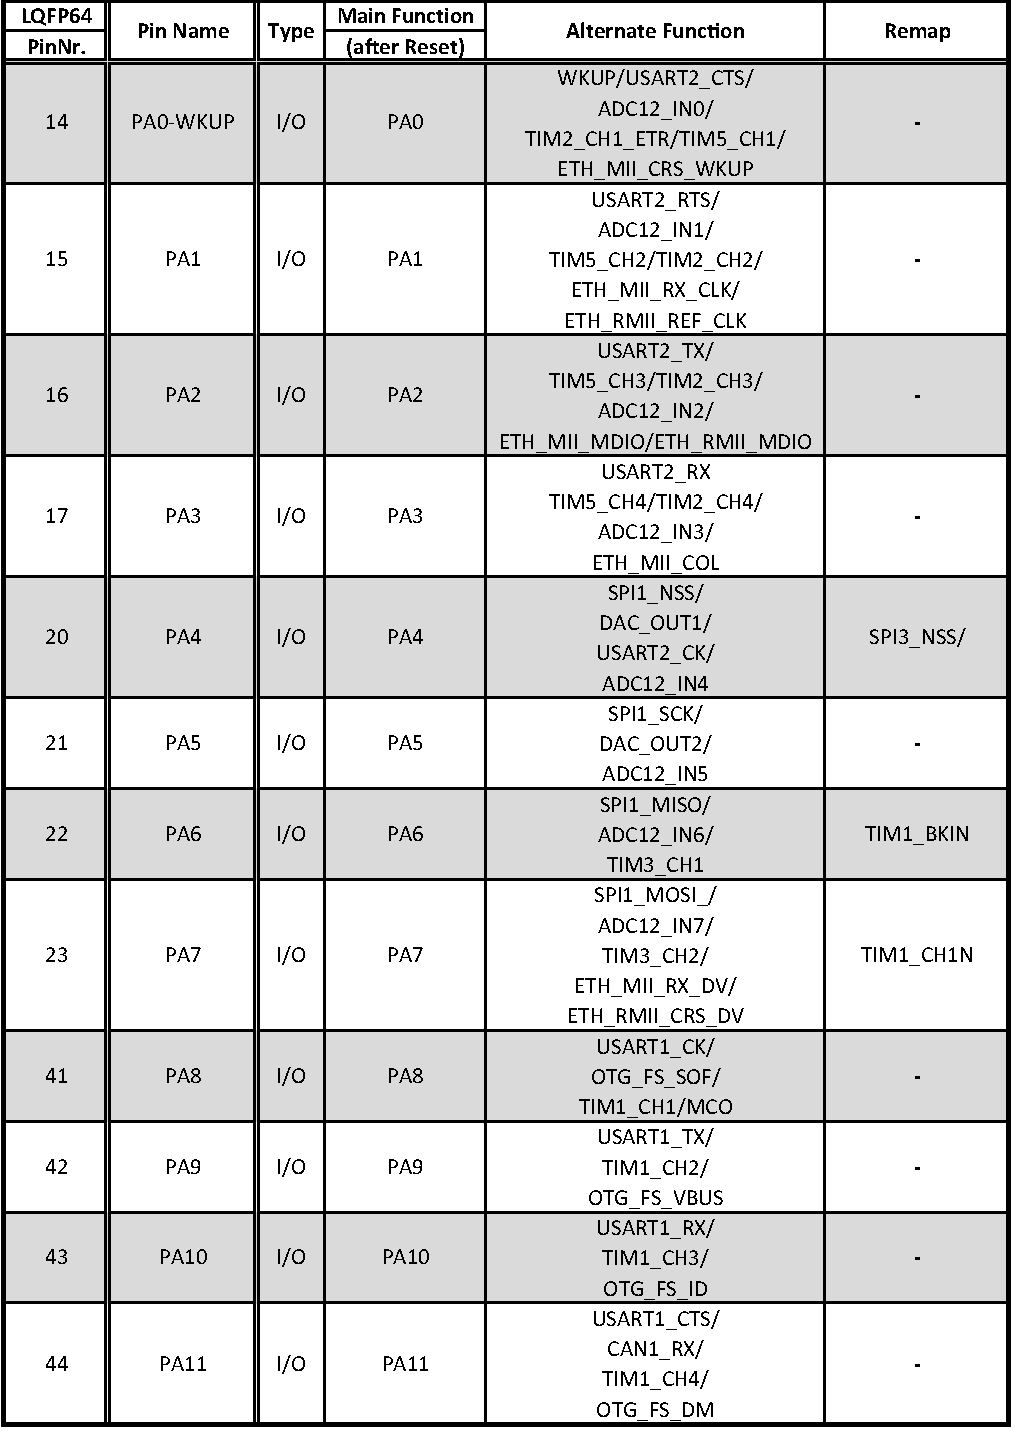
\includegraphics[width=0.8\textwidth]{Schuh/Pictures/Pinbelegung1}
    \caption[Pinbelegung des Prozessors]{Pinbelegung des Prozessors \cite{stm:stm32f107rc}}
    \label{tab:coremodul-cpupins}
\end{table}
\begin{table}[htb]\ContinuedFloat
    \centering
    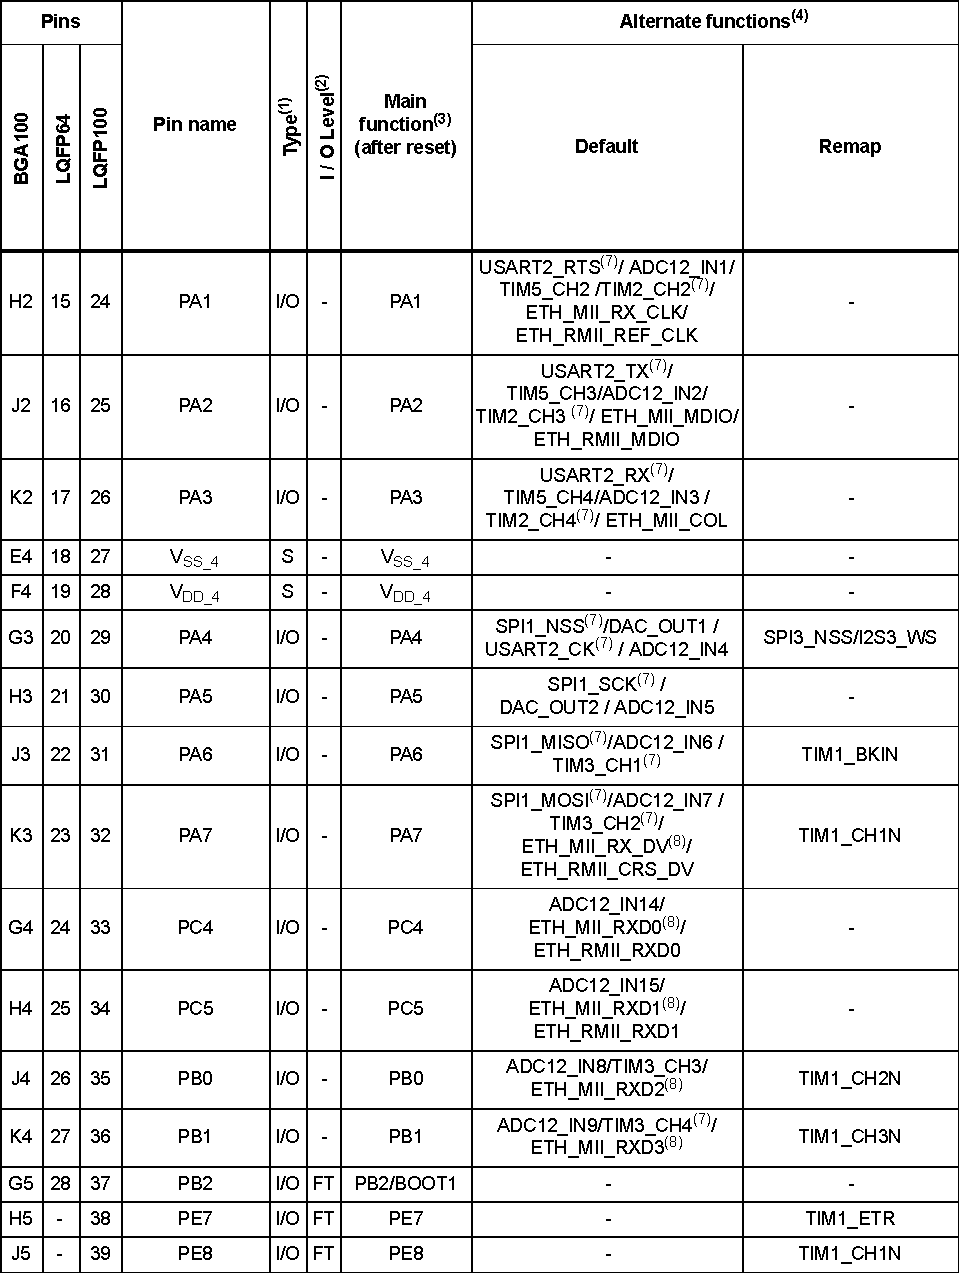
\includegraphics[width=0.8\textwidth]{Schuh/Pictures/Pinbelegung2}
    \caption[Pinbelegung des Prozessors]{Pinbelegung des Prozessors \cite{stm:stm32f107rc}}
\end{table}
\begin{table}[htb]\ContinuedFloat
    \centering
    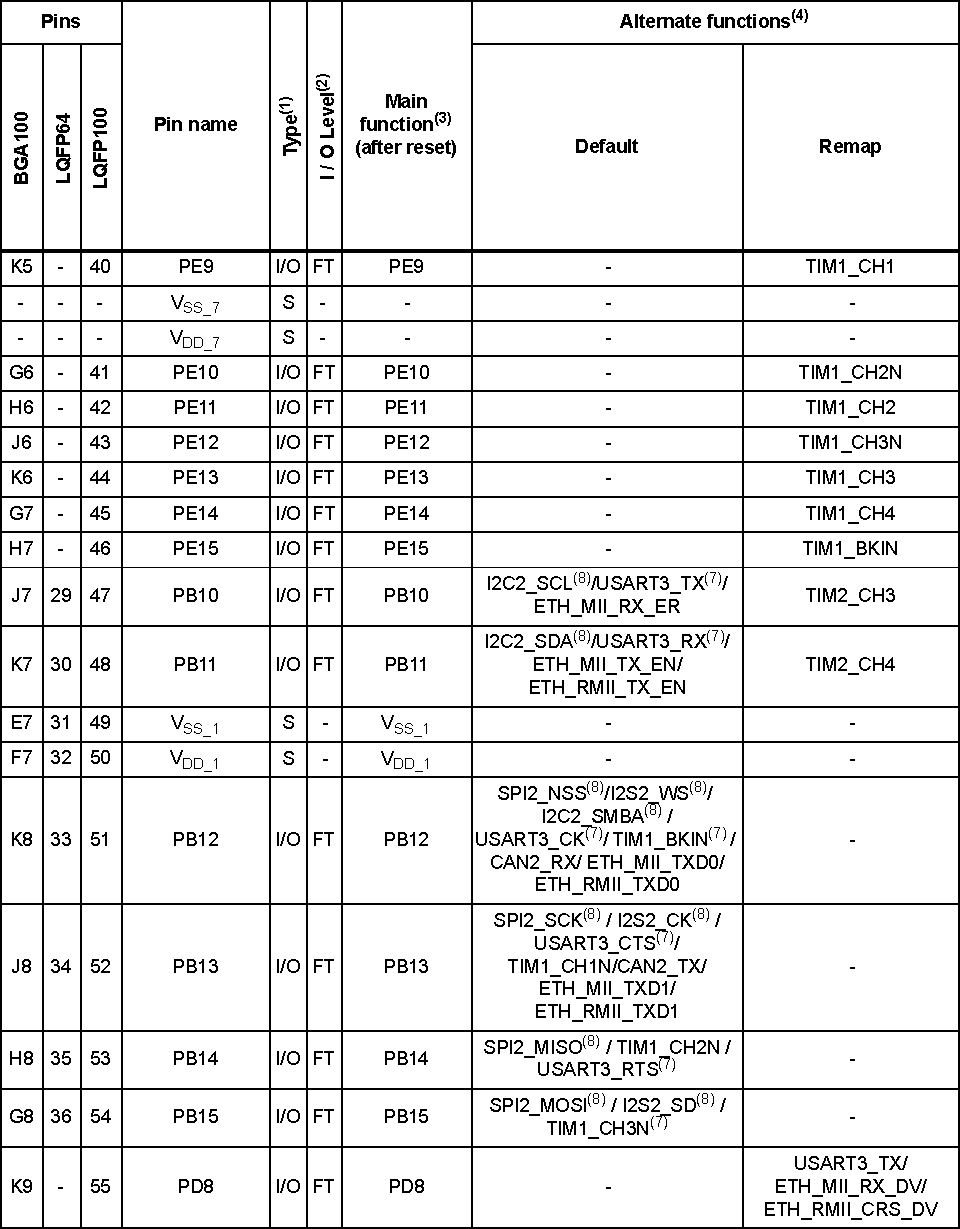
\includegraphics[width=0.8\textwidth]{Schuh/Pictures/Pinbelegung3}
    \caption[Pinbelegung des Prozessors]{Pinbelegung des Prozessors \cite{stm:stm32f107rc}}
\end{table}
\begin{table}[htb]\ContinuedFloat
    \centering
    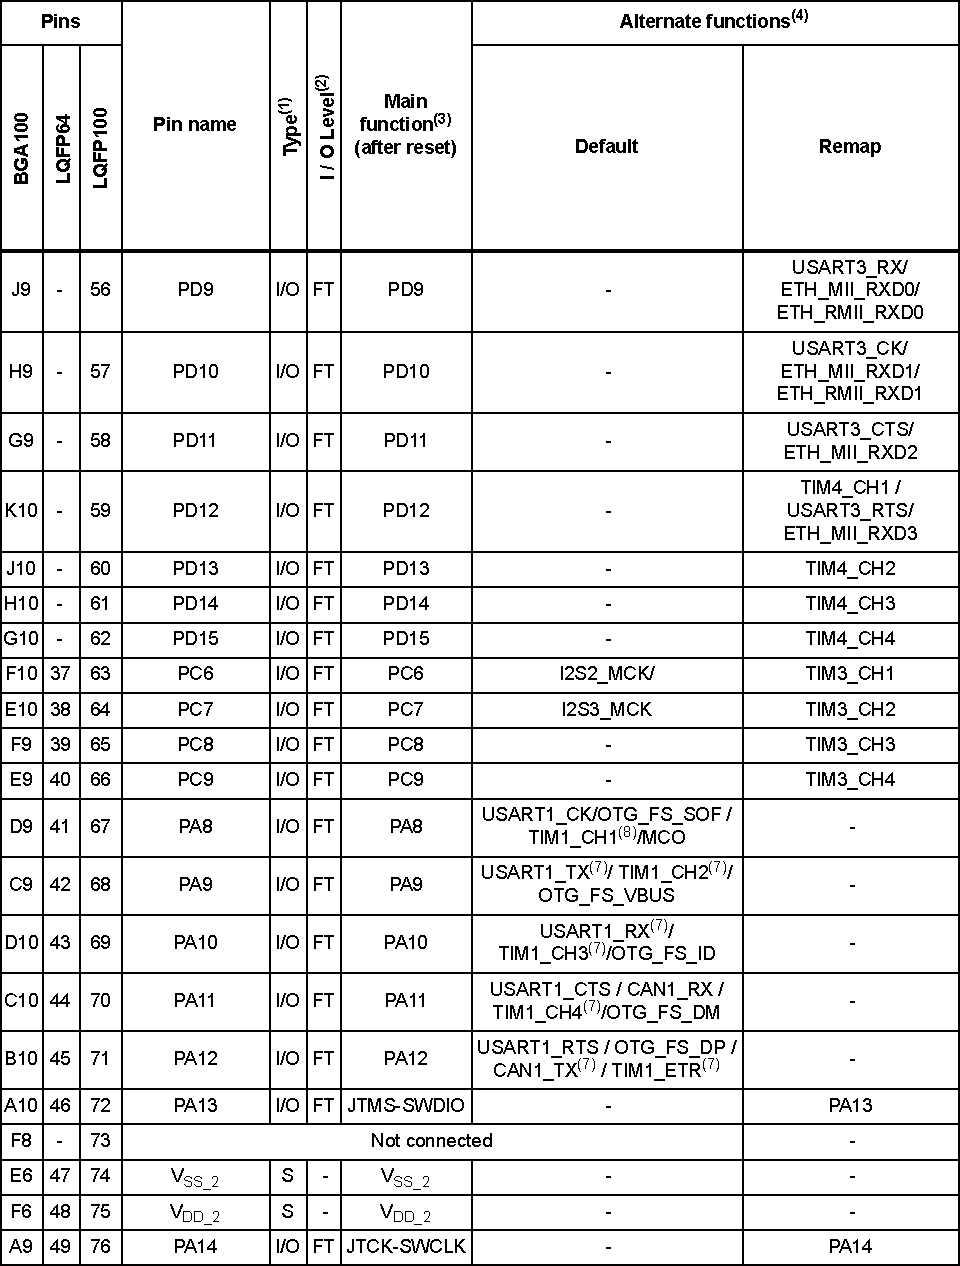
\includegraphics[width=0.8\textwidth]{Schuh/Pictures/Pinbelegung4}
    \caption[Pinbelegung des Prozessors]{Pinbelegung des Prozessors \cite{stm:stm32f107rc}}
\end{table}
\begin{table}[htb]\ContinuedFloat
    \centering
    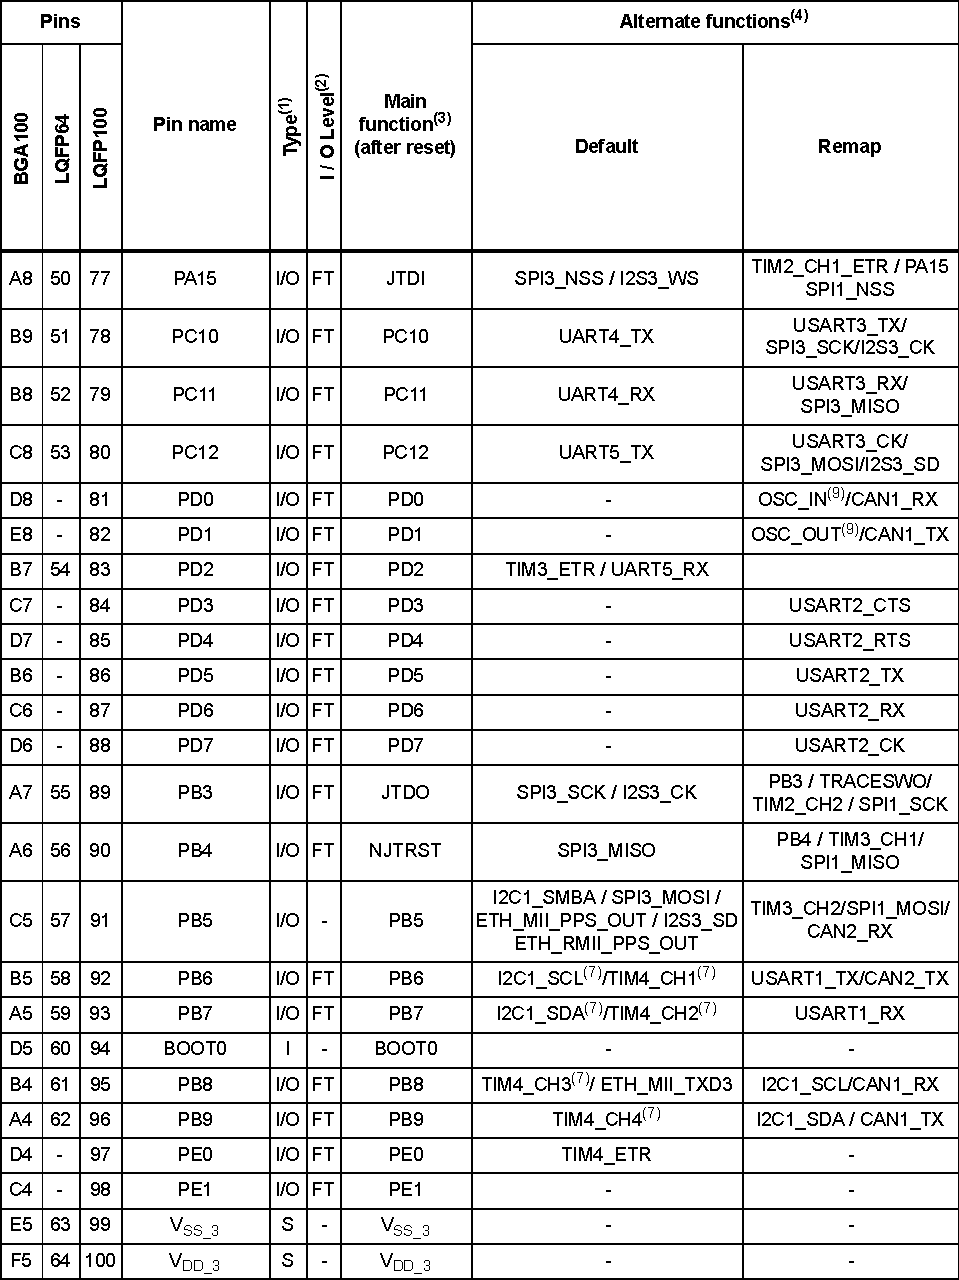
\includegraphics[width=0.8\textwidth]{Schuh/Pictures/Pinbelegung5}
    \caption[Pinbelegung des Prozessors]{Pinbelegung des Prozessors \cite{stm:stm32f107rc}}
\end{table}

\subsection{Portbelegungsplan}
\label{sec:coremodul-portbelegung}
\tabpdf{coremodul-portbelegung}{Portbelegungsplan des Core-Moduls}{Portbelegungsplan des \gls{Core-Modul}s}{0.5\textwidth}{Schuh/Pictures/Portbelegung}

\subsection{Gesamtschaltung}
\label{sec:coremodul-schaltung}
\fig{coremodul-gesamtschaltung}{Gesamtschaltung des Core-Moduls}{Gesamtschaltung des \gls{Core-Modul}s}{0.8\textwidth}{Schuh/Pictures/SchaltungCM}

\subsubsection{Programmierung mit ST-Link V2}
\label{sec:coremodul-stlink}
Zur Programmierung und zum \gls{Debugging} des neuen \gls{ARM}-\gls{Minimalsystem}s sollte ein \textbf{ST-Link V2 Mini} (\fref{fig:coremodul-stlink}) verwendet werden. Dieser Programmer besitzt eine verpolungssichere zweireihige Stiftreihe, welche es ermöglicht Programme mit Hilfe von \gls{SWD} auf den Microcontroller zu übertragen oder diese zu debuggen. Darüber hinaus ist der ST-Link V2 Mini der Lieferant der Hauptversorgungsspannung von \unit{+5}{\volt}.

Um den ST-Link V2 Mini und den Microcontroller im Falle eines Kurzschlusses zwischen der Versorgungsspannung und Masse zu schützen wurde eine Schottky-Diode (\fref{fig:coremodul-swd}, V1), mit einem maximalen Durchflussstrom von \unit{1}{\ampere}, vorgesehen. Um die Verpolungssicherheit des ST-Link V2 Mini zu gewährleisten, wurde eine zweireihige Buchsenleiste mit Nase (\fref{fig:coremodul-swd}, X1; \fref{fig:coremodul-stlinkbuchse}) verbaut, welche eine Verpolung des ST-Links unmöglich macht.

\fig{coremodul-stlink}{ST-Link V2 Mini}{ST-Link V2 Mini}{0.5\textwidth}{Schuh/Pictures/STLink}

\begin{figure}[htb]
    \centering
    \subfloat[Schematic\label{fig:coremodul-swd-schem}]{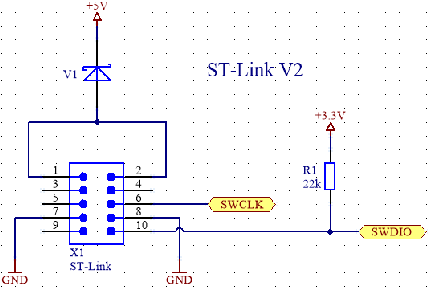
\includegraphics[width=.4\linewidth]{Schuh/Pictures/SchaltungSWD}}\qquad
\subfloat[Hardware\label{fig:coremodul-swd-hard}]{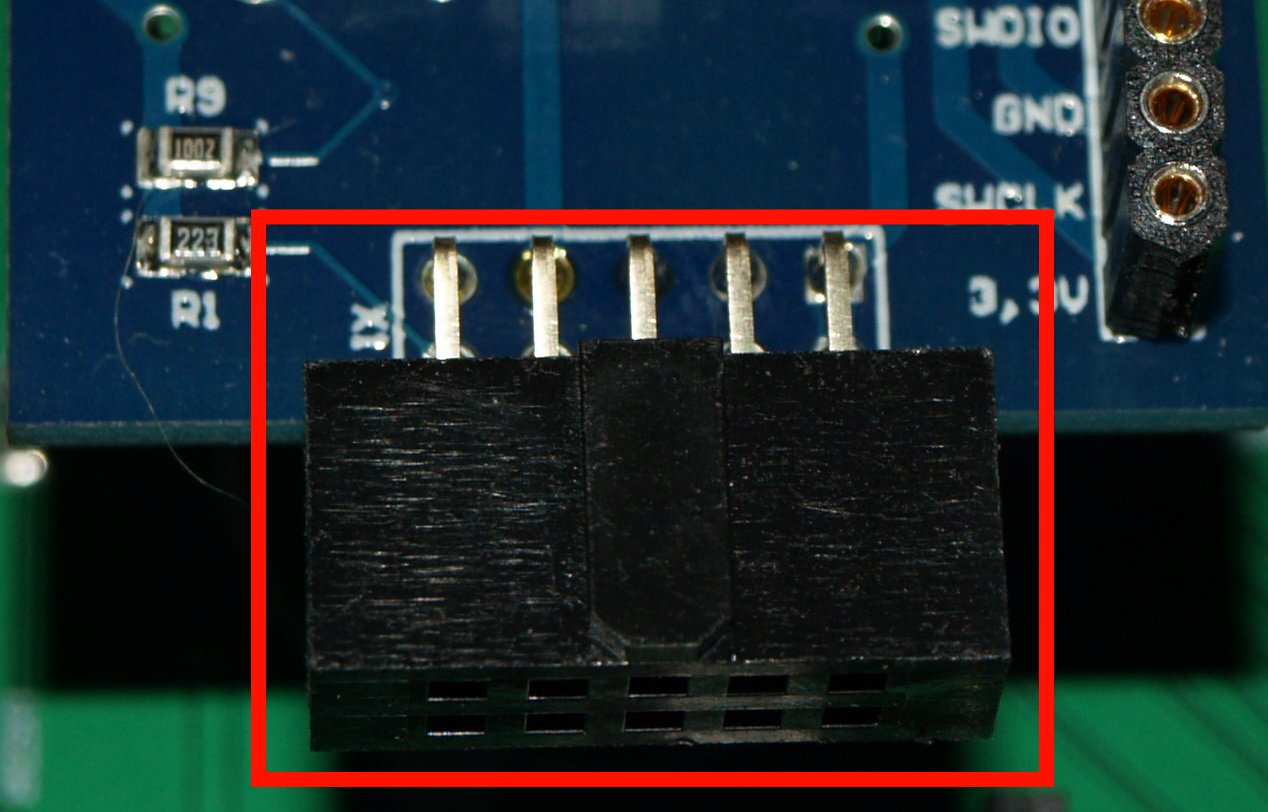
\includegraphics[width=.4\linewidth,angle=270]{Schuh/Pictures/core-stlink}}\qquad
    \caption[ST-Link Schaltung des Core-Moduls]{ST-Link Schaltung des \gls{Core-Modul}s}
    \label{fig:coremodul-swd}
\end{figure}

\fig{coremodul-stlinkbuchse}{Buchse mit Nase}{Buchse mit Nase}{0.5\textwidth}{Schuh/Pictures/STLinkBuchse}

\subsubsection{SWD-Adapter}
Der als Buchsenleiste ausgeführte SWD-Adapter (\fref{fig:coremodul-swd2}, X4), erfüllt vom Prinzip her die gleiche Funktion wie der bereits in \fref{sec:coremodul-stlink} beschriebene Stecker für den ST-Link V2 Mini. Dieser ermöglicht lediglich Kompatibilität zu anderen SWD-Programmern und Debuggern, welche diesen Stecker nicht besitzen.

\begin{figure}[htb]
    \centering
    \subfloat[Schematic\label{fig:coremodul-swd2-schem}]{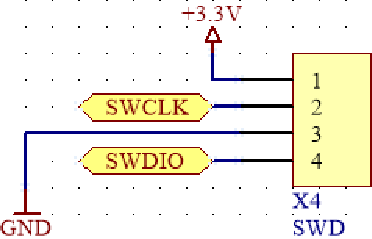
\includegraphics[width=.4\linewidth]{Schuh/Pictures/SchaltungSWD2}}\qquad
    \subfloat[Hardware\label{fig:coremodul-swd2-hard}]{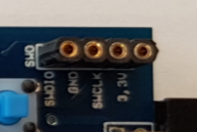
\includegraphics[width=.4\linewidth]{Schuh/Pictures/core-swd}}\qquad
    \caption[SWD-Schaltung des Core-Moduls]{SWD-Schaltung des \gls{Core-Modul}s}
    \label{fig:coremodul-swd2}
\end{figure}

\subsubsection{USART 1}
Die Buchsenleiste (\fref{fig:coremodul-uart}, X3) dient hauptsächlich zur seriellen Kommunikation. Die Pinanordnung wurde so gewählt, dass die Kommunikation entweder kabelgebunden, über den \gls{USB-to-UART} Adapter, oder alternativ über ein HC-06 Bluetooth Modul erfolgen kann.

\begin{figure}[htb]
    \centering
    \subfloat[Schematic\label{fig:coremodul-uart-schem}]{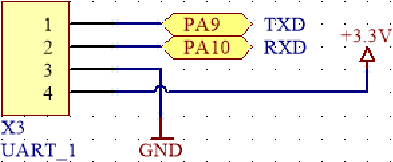
\includegraphics[width=.4\linewidth]{Schuh/Pictures/SchaltungUART}}\qquad
    \subfloat[Hardware\label{fig:coremodul-uart-hard}]{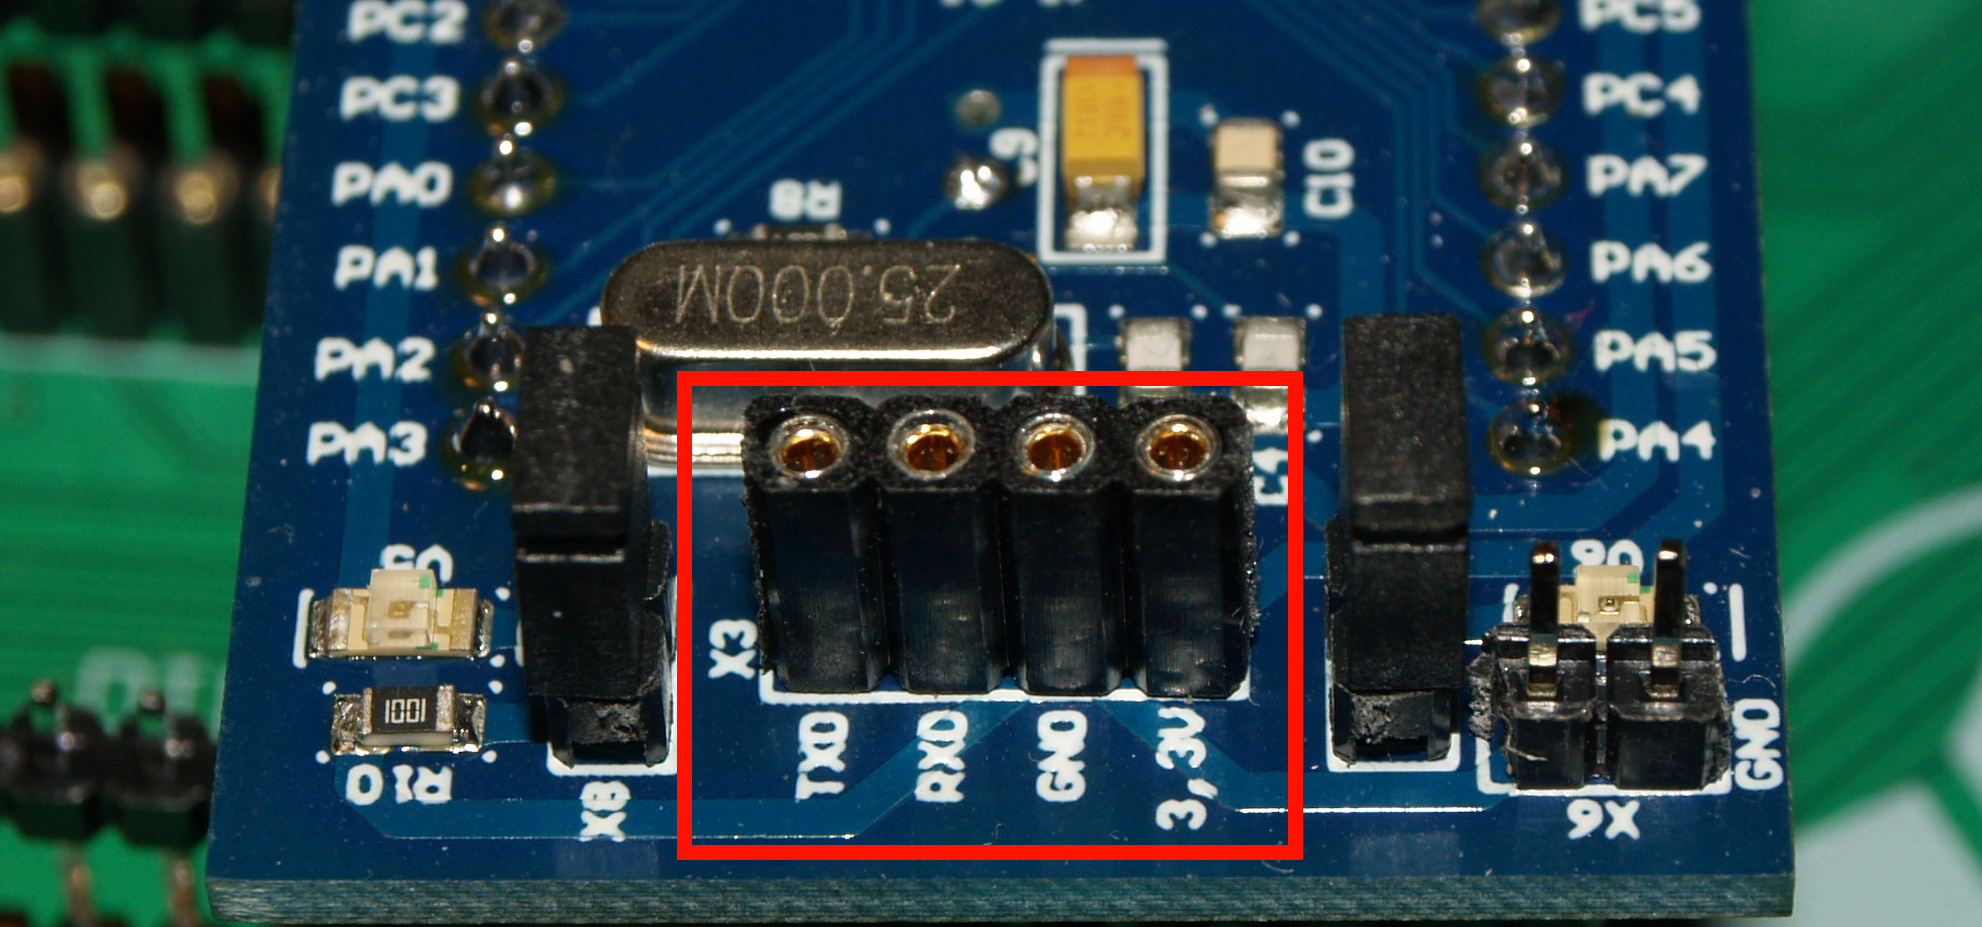
\includegraphics[angle=90,width=.4\linewidth]{Schuh/Pictures/core-uart}}\qquad
    \caption[UART-Schaltung des Core-Moduls]{UART-Schaltung des \gls{Core-Modul}s}
    \label{fig:coremodul-uart}
\end{figure}

\subsubsection{Bootkonfiguration}
Mit Hilfe des zweireihigen Bootjumpers (\fref{fig:coremodul-boot}, X5) kann der Benutzter entscheiden von welchem Speichermedium der Cortex booten soll.

Die Standardkonfiguration sieht vor, dass man vom Flash-Speicher bootet. Daher muss, wie in \fref{tab:coremodul-boot} beschrieben, Boot 0 auf GND gesetzt werden und Boot 1 auf +3.3V.

\fig{coremodul-boot}{Boot-Schaltung des Core-Moduls}{Boot-Schaltung des \gls{Core-Modul}s}{0.5\textwidth}{Schuh/Pictures/SchaltungBoot}
\tab{coremodul-boot}{Bootkonfigurationen des Core-Moduls}{Bootkonfigurationen des \gls{Core-Modul}s}{|c|c|p{10cm}|}{
    \hline
    \textbf{Boot 0} & \textbf{Boot 1} & \textbf{Funktion}\\
    \hline
    \unit{+3,3}{\volt} & \unit{+3,3}{\volt} & Booten von SRAM\\
    \hline
    \unit{+3,3}{\volt} & GND & Booten von Systemspeicher\\
    \hline
    GND & x & Booten von Flash-Speicher\\
    \hline
}

\subsubsection{Reset}
Der Kurzhubtaster (\fref{fig:coremodul-reset}, S2) dient zum Reset des \gls{Core-Modul}s. Mit Hilfe dieses ist ein erneuter Programmstart möglich, da er den Pin des low-aktiven Reset gegen Masse zieht. Gegebenenfalls angeschlossene Arduino-Shields werden mit diesem Taster ebenfalls zurückgesetzt.

\begin{figure}[htb]
    \centering
    \subfloat[Schematic\label{fig:coremodul-reset-schem}]{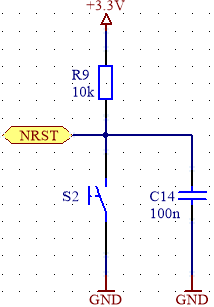
\includegraphics[width=.4\linewidth]{Schuh/Pictures/schaltung-reset}}\qquad
    \subfloat[Hardware\label{fig:coremodul-reset-hard}]{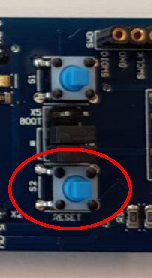
\includegraphics[width=.4\linewidth]{Schuh/Pictures/core-reset}}\qquad
    \caption[Reset-Schaltung des Core-Moduls]{Reset-Schaltung des \gls{Core-Modul}s}
    \label{fig:coremodul-reset}
\end{figure}

\subsubsection{\unit{5}{\volt} Spannungsversorgung}
Die \unit{+5}{\volt} Spannungsversorgung für das \gls{Core-Modul} kann auf zwei verschiedenen Wegen bezogen werden. Entweder man verwendet den ST-Link V2 Mini als \unit{5}{\volt} Spannungsversorgung (\fref{fig:coremodul-swd}, X1), wie bereits in \fref{sec:coremodul-stlink} beschrieben, oder man speist die \unit{+5}{\volt} Versorgung über den \unit{5}{\volt}-Pin am DIL-Adapter (\fref{fig:coremodul-spannung}, X2) ein.

\fig{coremodul-spannung}{Spannungsversorgungsschaltung des Core-Moduls}{Spannungsversorgungsschaltung des \gls{Core-Modul}s}{0.5\textwidth}{Schuh/Pictures/schaltung-spannung}

\subsubsection{Batterieversorgung}
An VB kann eine \unit{3,3}{\volt}-Batterie angeschlossen werden, damit die \gls{RTC} auch dann mit Spannung versorgt ist, wenn der Cortex-M3 außer Betrieb ist. Darüber hinaus wird im Falle des stromsparenden Deep-Sleep-Mode des Cortex-M3 ebenfalls eine Puffer-Batterie benötigt. Die Schottky-Diode (\fref{fig:coremodul-batterie}, V4) soll verhindern, dass die Batterie welche die \gls{RTC} des Cortex betreiben soll, nicht geladen wird. In den meisten Fällen handelt es sich bei dieser Batterie um eine Knopfzelle, welche häufig nicht wiederaufladbar ist. Die Schottky-Diode (\fref{fig:coremodul-batterie}, V3) soll verhindern, dass die Batteriespannung der \unit{3,3}{\volt}-Knopfzelle, mit der über einen Linearregler generierten Versorgungsspannung des Prozessors verbunden wird.

\fig{coremodul-batterie}{Batterieversorgungsschaltung des Core-Moduls}{Batterieversorgungsschaltung des \gls{Core-Modul}s}{0.5\textwidth}{Schuh/Pictures/schaltung-batterie}

\subsubsection{\unit{3,3}{\volt} Fixspannungsregler}
Zur Generierung der für den Prozessor erforderlichen Betriebsspannung wurde ein \unit{3,3}{\volt}-Linearregler (\fref{fig:coremodul-fix}, U2) verwendet, welcher die Eingangsspannung von \unit{+5}{\volt} auf \unit{+3,3}{\volt} herabsetzt. Bei Verwendung eines Linearreglers ist zu beachten, dass dieser die Spannungsdifferenz zwischen Ausgangsspannung und Eingangsspannung in Wärme umwandelt. Daher sollten keine temperaturempfindlichen Bauteile in dessen Nähe platziert werden. Zur Überprüfung ob das Modul mit der Betriebsspannung von \unit{+5}{\volt} versorgt wird, wurde die LED (\fref{fig:coremodul-fix}, V4) zur optischen Kontrolle eingebaut. Wenn das Modul mit Spannung versorgt wird, leuchtet diese. Zur Überprüfung ob der Prozessor mit seiner Betriebsspannung von \unit{3,3}{\volt} versorgt wird, wurde die LED (\fref{fig:coremodul-fix}, V6) zur optischen Kontrolle eingebaut. Wenn der Prozessor mit Spannung versorgt wird, leuchtet sie. Um den Stromverbrauch des \gls{Core-Modul}s im Low-Power Modus weiter zu senken, können die LEDs mit Hilfe von Jumpern außer Betrieb gesetzt werden.

\begin{figure}[htb]
    \centering
    \subfloat[Schematic\label{fig:coremodul-fix-schem}]{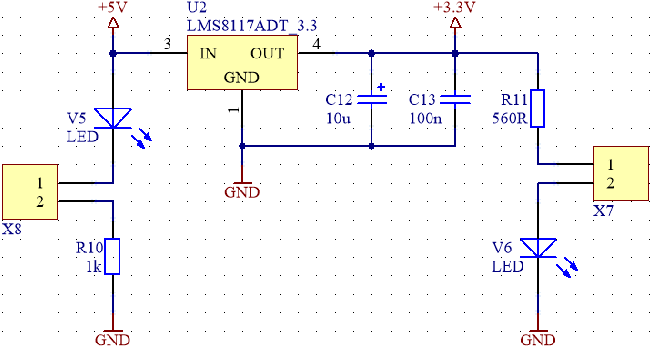
\includegraphics[width=.75\linewidth]{Schuh/Pictures/schaltung-fix}}\qquad
    \subfloat[Hardware\label{fig:coremodul-fix-hard}]{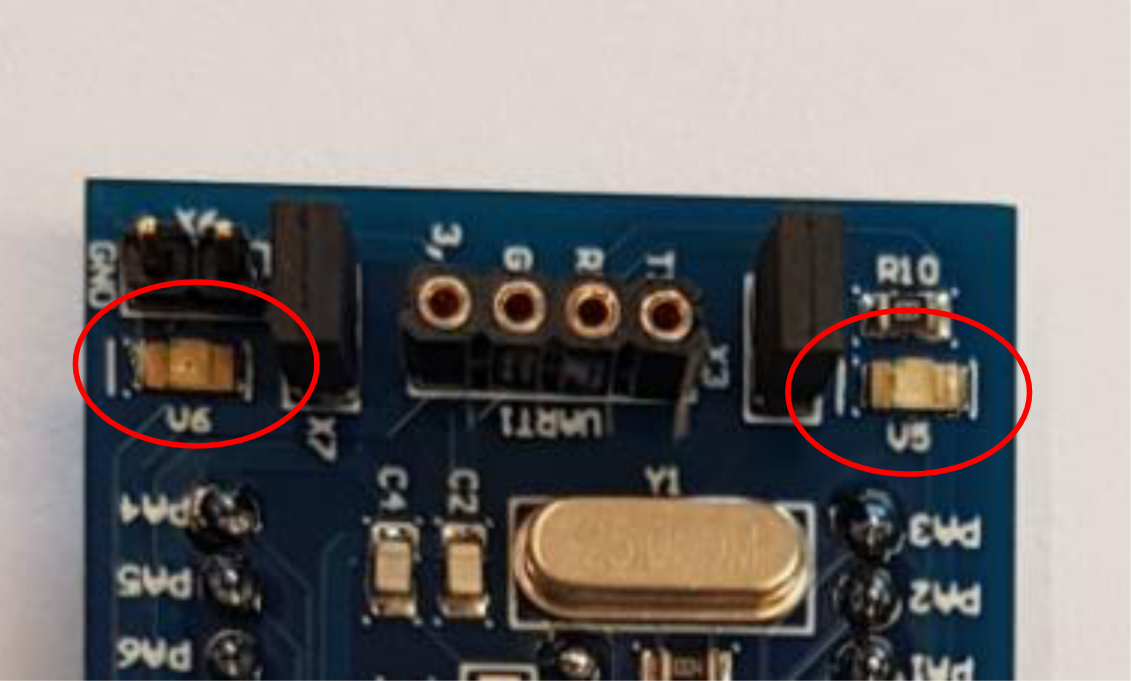
\includegraphics[width=.4\linewidth]{Schuh/Pictures/core-fix}}\qquad
    \caption[Fixspannungsregler des Core-Moduls]{Fixspannungsregler des \gls{Core-Modul}s}
    \label{fig:coremodul-fix}
\end{figure}


\subsubsection{Prozessor}
Das Schaltplansymbol für den Prozessor (\fref{fig:coremodul-prozessor}, U1) zeigt den im Schematic verwendeten Bauteil. Alle wichtigen Detailinformationen über den Prozessor wurden bereits in \fref{sec:coremodul-prozessor} behandelt.

\begin{figure}[htb]
    \centering
    \subfloat[Schematic\label{fig:coremodul-prozessor-schem}]{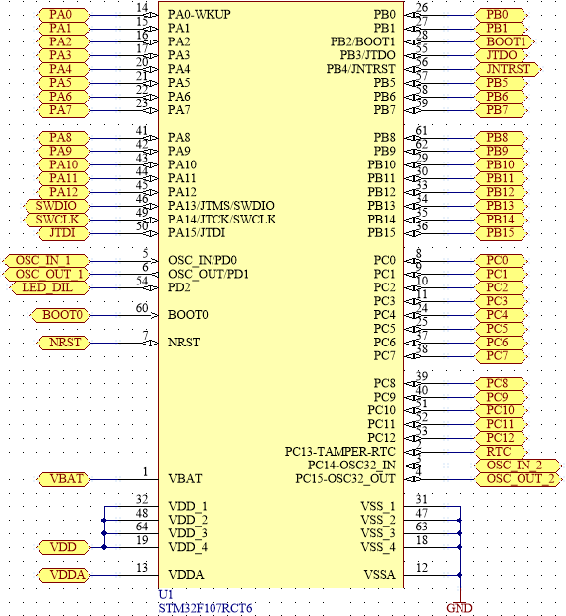
\includegraphics[width=.75\linewidth]{Schuh/Pictures/schaltung-prozessor}}\qquad
    \subfloat[Hardware\label{fig:coremodul-prozessor-hard}]{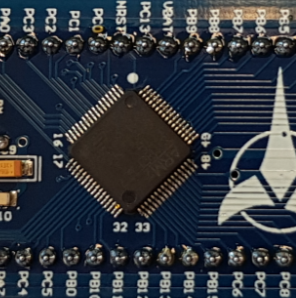
\includegraphics[width=.4\linewidth]{Schuh/Pictures/core-prozessor}}\qquad
    \caption[Prozessor des Core-Moduls]{Prozessor des \gls{Core-Modul}s}
    \label{fig:coremodul-prozessor}
\end{figure}

\subsubsection{Stützkondensatoren}
Während des laufenden Betriebs eines Microcontrollers benötigt dieser unterschiedlich viel Strom. Um auf diese Stromspitzen reagieren zu können, wurden Stützkondensatoren vorgesehen, damit es nicht zu Absturz des Programmes oder zu anderen Problemen durch Spannungseinbrüche kommt. Die Stützkondensatoren (\fref{fig:coremodul-kond}: C5, C6, C7 und C8) können daher die in ihnen gespeicherte Ladung bei stark wechselnden Stromaufnahmen abgeben und dadurch eine ordnungsmäßige Versorgung des Prozessors gewährleisten.

\fig{coremodul-kond}{Stützkondensatoren des Core-Moduls}{Stützkondensatoren des \gls{Core-Modul}s}{0.5\textwidth}{Schuh/Pictures/schaltung-kond}

\subsubsection{DIL-Adapter}
Das Schaltplansymbol des DIL-Adapters (\fref{fig:coremodul-dil}, X2) zeigt das Pinning, welches hardwaremäßig auf den zwei getrennten Buchsenleisten auf der Leiterkarte ausgeführt wurde.

\fig{coremodul-dil}{DIL-Adapter des Core-Moduls}{DIL-Adapter des \gls{Core-Modul}s}{0.5\textwidth}{Schuh/Pictures/schaltung-dil}

\subsubsection{Schwingquarze}
Das \gls{Core-Modul} besitzt standardmäßig zwei verschiedene Taktquellen. Diese bestehen aus einem 25MHz Quarz (\fref{fig:coremodul-quarz}, Y1), welcher für die Taktfrequenz des Prozessors zuständig ist, und einem 32kHz Quarz (\fref{fig:coremodul-quarz}, Y2), welcher für die interne \gls{RTC} zur Verfügung steht.

\fig{coremodul-quarz}{Schwingquarze des Core-Moduls}{Schwingquarze des \gls{Core-Modul}s}{0.75\textwidth}{Schuh/Pictures/schaltung-quarz}

\subsubsection{Taster}
Auf dem \gls{Core-Modul} wurde ein Kurzhubtaster (\fref{fig:coremodul-taster}, S1) vorgesehen, dessen Funktion nach belieben ausprogrammiert werden kann.

\begin{figure}[htb]
    \centering
    \subfloat[Schematic\label{fig:coremodul-taster-schem}]{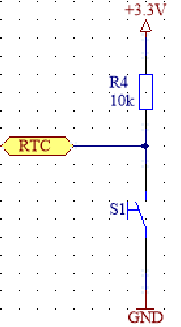
\includegraphics[width=.25\linewidth]{Schuh/Pictures/schaltung-taster}}\qquad
    \subfloat[Hardware\label{fig:coremodul-taster-hard}]{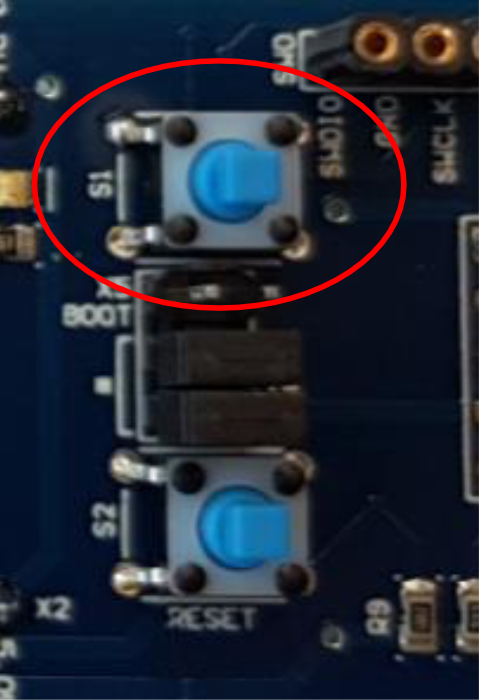
\includegraphics[width=.25\linewidth]{Schuh/Pictures/core-taster}}\qquad
    \caption[Taster des Core-Moduls]{Taster des \gls{Core-Modul}s}
    \label{fig:coremodul-taster}
\end{figure}

\subsubsection{LED}
Auf dem \gls{Core-Modul} wurde eine LED (\fref{fig:coremodul-led}, V2) vorgesehen, deren Funktion nach belieben ausprogrammiert werden kann.

\begin{figure}[htb]
    \centering
    \subfloat[Schematic\label{fig:coremodul-led-schem}]{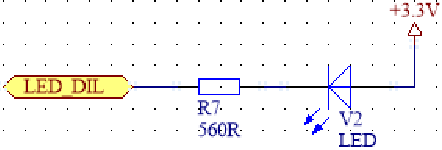
\includegraphics[width=.4\linewidth]{Schuh/Pictures/schaltung-led}}\qquad
    \subfloat[Hardware\label{fig:coremodul-led-hard}]{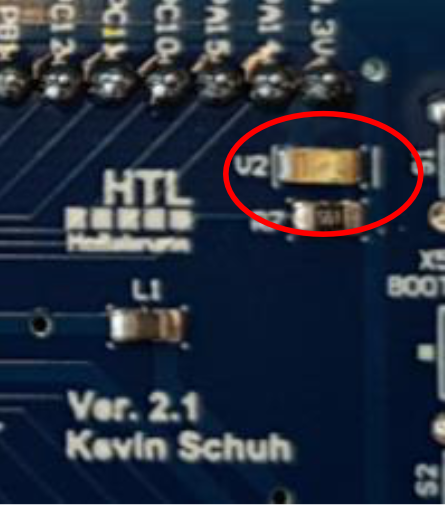
\includegraphics[width=.25\linewidth]{Schuh/Pictures/core-led}}\qquad
    \caption[LED des Core-Moduls]{LED des \gls{Core-Modul}s}
    \label{fig:coremodul-led}
\end{figure}

\subsubsection{Masseschleife}
Um das Messen mit einem Oszilloskop oder anderen Messgeräten zu vereinfachen wurde eine Masseschleife (\fref{fig:coremodul-masse}, X6) auf dem \gls{Core-Modul} realisiert.

\begin{figure}[htb]
    \centering
    \subfloat[Schematic\label{fig:coremodul-masse-schem}]{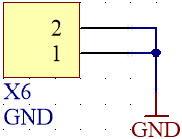
\includegraphics[width=.25\linewidth]{Schuh/Pictures/schaltung-masse}}\qquad
    \subfloat[Hardware\label{fig:coremodul-masse-hard}]{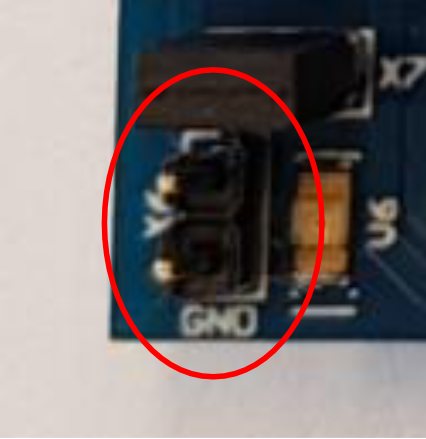
\includegraphics[width=.25\linewidth]{Schuh/Pictures/core-masse}}\qquad
    \caption[Masseschleife des Core-Moduls]{Masseschleife des \gls{Core-Modul}s}
    \label{fig:coremodul-masse}
\end{figure}

\subsection{Leiterplattenlayout}
\label{sec:coremodul-leiterplattenlayout}
\subsubsection{Bauteilseite}
\fig{coremodul-lbauteilseite}{Layout Bauteilseite des Core-Moduls}{Layout Bauteilseite des \gls{Core-Modul}s}{\textwidth}{Schuh/Pictures/core-lbauteilseite}

\subsubsection{Lötseite}
\fig{coremodul-llötseite}{Layout Lötseite des Core-Moduls}{Layout Lötseite des \gls{Core-Modul}s}{\textwidth}{Schuh/Pictures/core-llotseite}

\subsection{Bestückungspläne}
\label{sec:coremodul-bestückungspläne}
\subsubsection{Bauteilseite}
\fig{coremodul-bbauteilseite}{Bestückungsplan Bauteilseite des Core-Moduls}{Bestückungsplan Bauteilseite des \gls{Core-Modul}s}{\textwidth}{Schuh/Pictures/core-bbauteilseite}

\subsubsection{Lötseite}
\fig{coremodul-blötseite}{Bestückungsplan Lötseite des Core-Moduls}{Bestückungsplan Lötseite des \gls{Core-Modul}s}{\textwidth}{Schuh/Pictures/core-blotseite}
\section{Basisplatine}
\label{sec:basisplatine}

\fig{core-modul}{Basisplatine}{\gls{Basisplatine}}{\textwidth}{Schuh/Pictures/basis}

\subsection{Allgemeines}
\label{sec:basisplatine-allgemeines}
Die \gls{Basisplatine} dient dazu dem \gls{Core-Modul} eine umfangreiche, moderne und jederzeit erneuerbare Peripherie bereit zu stellen, um verschiedene Anwendungskonzepte schnell und einfach evaluieren zu können. Darüber hinaus soll mit Hilfe der \gls{Basisplatine} eine Versorgung und Programmierung des \gls{Core-Modul}s möglich sein. Durch Verwendung des Arduino-Shield-Konnektors können alle am Markt verfügbaren Arduino-Shields verwendet werden, daher kann man jederzeit Hardwarekomponenten tauschen oder selbst entwickeln.

\subsection{Schnittstellen}
\label{sec:basisplatine-schnittstellen}

Die \gls{Basisplatine} verfügt über mehrere in \fref{tab:basisplatine-schnittstellen} angegebene Schnittstellen. In \fref{fig:basisplatine-plan} dargestellt wie diese auf der \gls{Basisplatine} platziert sind.

\tab{basisplatine-schnittstellen}{Schnittstellen der Basisplatine}{Schnittstellen der \gls{Basisplatine}}{|c|p{10cm}|}{
    \hline
    \textbf{Schnittstelle} & \textbf{Funktion}\\
    \hline
    USART 1 & Ansteuerung von HC-06, HC-12, \gls{USB-to-UART}-Adapter, MAX232\\
    \hline
    USART 2 & Ansteuerung von ESP8266, XBee-Pro\\
    \hline
    USART 3 & Ansteuerung von Nextion-Display\\
    \hline
    SPI 1 & \\
    \hline
    \IIC{} 1 & \\
    \hline
    SWD & Programmierung auf Basis von \gls{SWD}\\
    \hline
    ST-Link V2 & Programmierung auf Basis von \gls{SWD}\\
    \hline
    JTAG & Programmierung auf Basis von \gls{JTAG}\\
    \hline
    DE-9 Buche & Ansteuerung von Nextion-Display\\
    \hline
    Arduino-Shield-Connector & Verwendung von diversen Arduino-Shields\\
    \hline
    Audio-Shield-Connector & Verwendung des HTL-internen Audio-Shields\\
    \hline
    Singe-Wire & Ansteuerung von Piezo, Temperatursensor, LFU, IR-Sensor, BMA020, EEPROM\\
    \hline
    USB-A & Spannungsversorgung, Datentransport\\
    \hline
    USB-B & Spannungsversorgung, Datentransport\\
    \hline
}

\fig{basisplatine-plan}{Übersichtsplan der Basisplatine}{Übersichtsplan der \gls{Basisplatine}}{\textwidth}{Schuh/Pictures/Basisplatine}

\subsection{Portbelegungsplan}
\label{sec:basisplatine-portbelegung}
\tabpdf{basisplatine-portbelegung}{Portbelegungsplan der Basisplatine}{Portbelegungsplan der \gls{Basisplatine}}{0.45\textwidth}{Schuh/Pictures/Basis-Portbelegung}

\subsubsection{ST-Link V2}
\label{sec:basisplatine-stlink}
Zur Programmierung und zum \gls{Debugging} des neuen \gls{ARM}-\gls{Minimalsystem}s sollte ein \textbf{ST-Link V2 Mini} verwendet werden. Dieser Programmer besitzt eine verpolungssichere zweireihige Stiftreihe, welche es ermöglicht Programme mit Hilfe von \gls{SWD} auf den Microcontroller zu übertragen oder diese zu debuggen. Darüber hinaus ist der ST-Link V2 Mini der Lieferant der Hauptversorgungsspannung von \unit{+5}{\volt}.

Um den ST-Link V2 Mini und den Microcontroller im Falle eines Kurzschlusses zwischen der Versorgungsspannung und Masse zu schützen wurde eine Schottky-Diode V16 (\fref{fig:basisplatine-swd}), mit einem maximalen Durchflussstrom von \unit{3}{\ampere}, vorgesehen.

\begin{figure}[H]
    \centering
    \subfloat[Schematic\label{fig:basisplatine-swd-schem}]{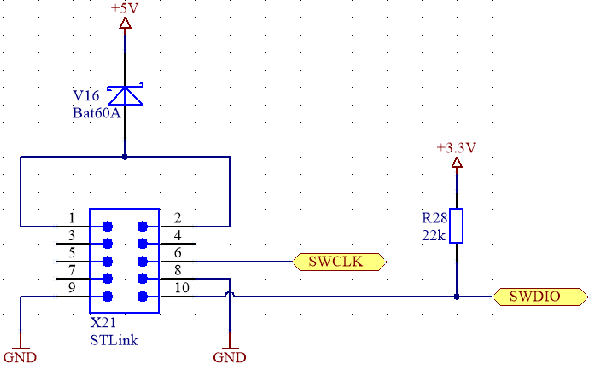
\includegraphics[width=.6\linewidth]{Schuh/Pictures/Basis-SWD}}\qquad
    \subfloat[Hardware\label{fig:basisplatine-swd-hard}]{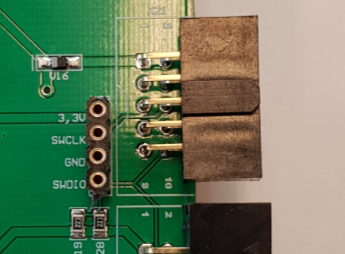
\includegraphics[width=.3\linewidth]{Schuh/Pictures/basis-stlink}}\qquad
    \caption[ST-Link Schaltung der Basisplatine]{ST-Link Schaltung der \gls{Basisplatine}}
    \label{fig:basisplatine-swd}
\end{figure}

\subsubsection{SWD-Adapter}
Der als Buchsenleiste ausgeführte SWD-Adapter X23 (\fref{fig:basisplatine-swd2}), erfüllt vom Prinzip her die gleiche Funktion wie der bereits in \fref{sec:basisplatine-stlink} beschriebene Stecker für den ST-Link V2 Mini. Dieser ermöglicht lediglich Kompatibilität zu anderen SWD-Programmern und Debuggern, welche diesen Stecker nicht besitzen.

\begin{figure}[H]
    \centering
    \subfloat[Schematic\label{fig:basisplatine-swd2-schem}]{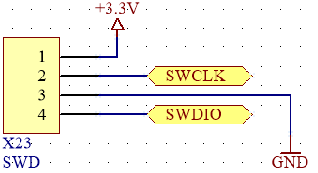
\includegraphics[width=.4\linewidth]{Schuh/Pictures/Basis-SWD2}}\qquad
    \subfloat[Hardware\label{fig:basisplatine-swd2-hard}]{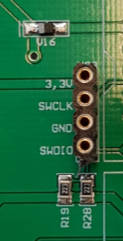
\includegraphics[width=.2\linewidth]{Schuh/Pictures/basis-swd}}\qquad
    \caption[SWD-Schaltung der Basisplatine]{SWD-Schaltung der \gls{Basisplatine}}
    \label{fig:basisplatine-swd2}
\end{figure}

\subsubsection{JTAG}
Zur Programmierung und zum \gls{Debugging} des neuen \gls{ARM}-\gls{Minimalsystem}s wurde aus kompatibilitätsgründen zum alten System zusätzlich vollwertige JTAG-Schnittstelle vorgesehen, um weiterhin mit Hilfe des ULINK/ME Adapters arbeiten zu können. Auch diese Schnittstelle besitzt eine verpolungssichere zweireihige Buchsenleiste X19 (\fref{fig:basisplatine-jtag}), welche es ermöglicht Programme mit Hilfe des JTAG-Protokolls auf den Microcontroller zu übertragen oder diese zu debuggen.

\begin{figure}[H]
    \centering
    \subfloat[Schematic\label{fig:basisplatine-jtag-schem}]{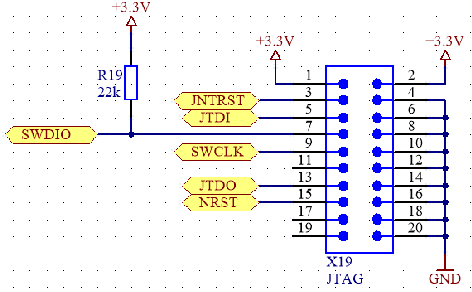
\includegraphics[width=.5\linewidth]{Schuh/Pictures/Basis-JTAG}}\qquad
    \subfloat[Hardware\label{fig:basisplatine-jtag-hard}]{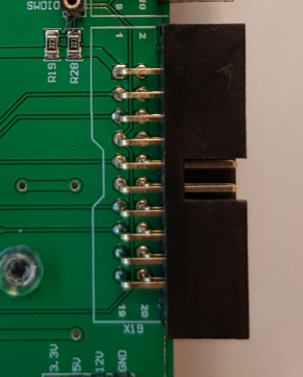
\includegraphics[width=.3\linewidth]{Schuh/Pictures/basis-jtag}}\qquad
    \caption[JTAG-Schaltung der Basisplatine]{JTAG-Schaltung der \gls{Basisplatine}}
    \label{fig:basisplatine-jtag}
\end{figure}

\subsubsection{Core-Modul-Adapter}
Das Schaltplansymbol des \gls{Core-Modul}s X20 (\fref{fig:basisplatine-core}) zeigt das Pinning, welches auf zwei Buchsenleisten auf der \gls{Basisplatine} herausgeführt wurde.

\begin{figure}[H]
    \centering
    \subfloat[Schematic\label{fig:basisplatine-core-schem}]{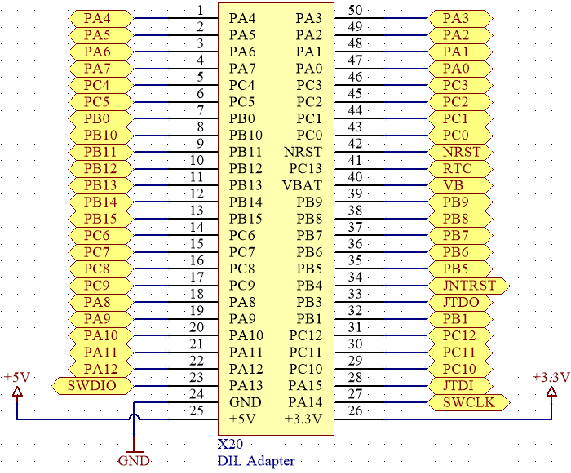
\includegraphics[width=.5\linewidth]{Schuh/Pictures/Basis-core}}\qquad
    \subfloat[Hardware\label{fig:basisplatine-core-hard}]{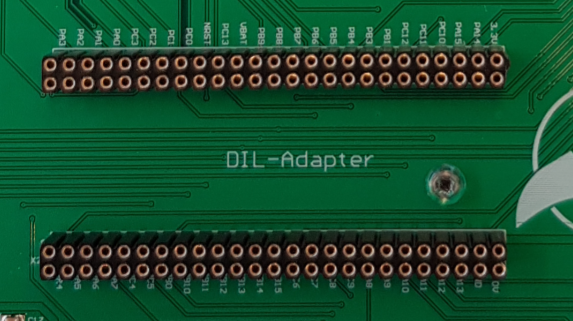
\includegraphics[width=.5\linewidth]{Schuh/Pictures/basis-core}}\qquad
    \caption[Core-Modul-Adapter der Basisplatine]{\gls{Core-Modul}-Adapter der \gls{Basisplatine}}
    \label{fig:basisplatine-core}
\end{figure}

\subsubsection{Audio-Adapter}
Der bereits in einer anderen Diplomarbeit realisierte Audio-Adapter kann auf der zweireihigen Buchsenleiste X24 (\fref{fig:basisplatine-audio}) aufgesteckt und anschließend betrieben werden.

\begin{figure}[H]
    \centering
    \subfloat[Schematic\label{fig:basisplatine-audio-schem}]{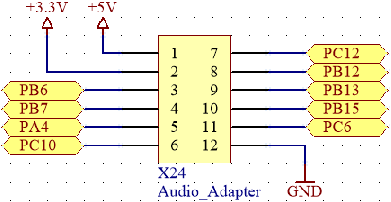
\includegraphics[width=.4\linewidth]{Schuh/Pictures/Basis-audio}}\qquad
    \subfloat[Hardware\label{fig:basisplatine-audio-hard}]{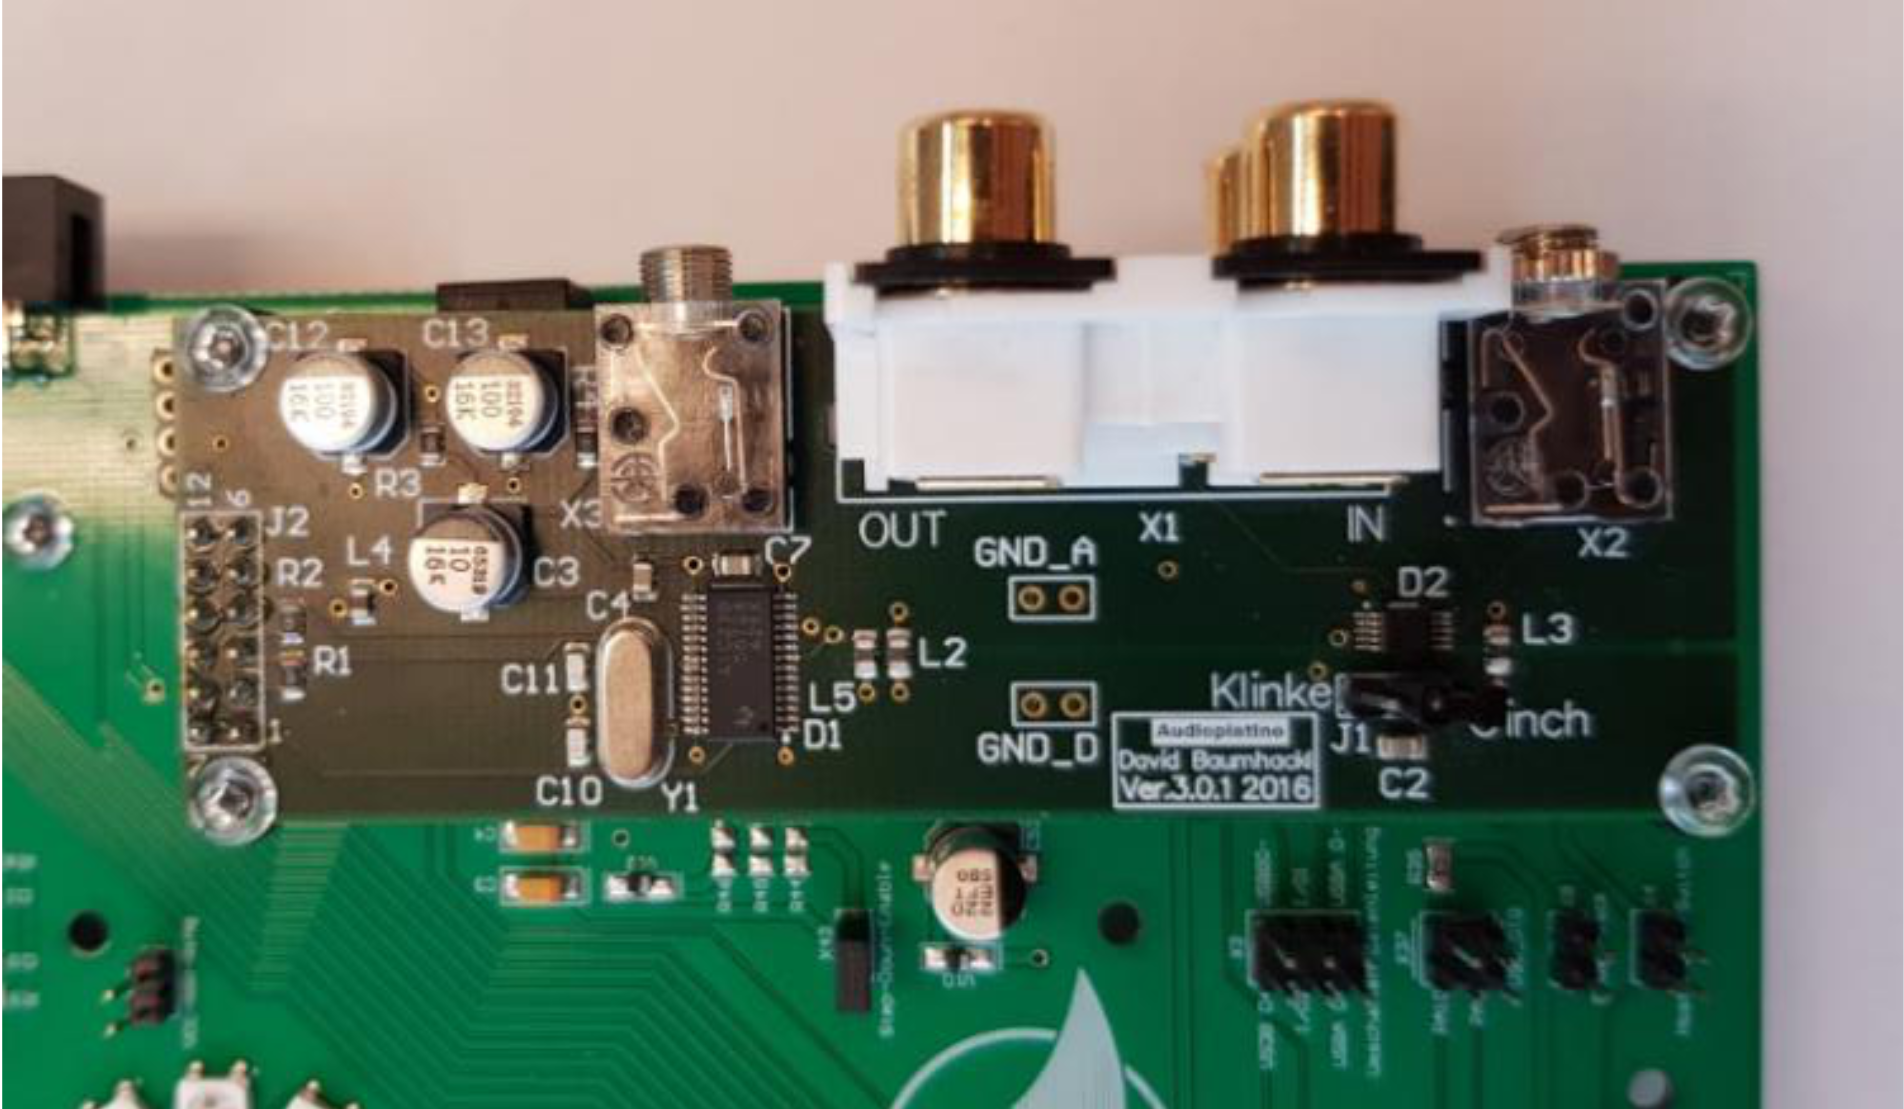
\includegraphics[width=.4\linewidth]{Schuh/Pictures/basis-audio}}\qquad
    \caption[Audio-Adapter der Basisplatine]{Audio-Adapter der \gls{Basisplatine}}
    \label{fig:basisplatine-audio}
\end{figure}

\subsubsection{LED-Array}
Auf der \gls{Basisplatine} wurde ein LED-Array realisiert, welches aus acht LEDs besteht und über die Portleitungen PC1 bis PC5 und PC7 bis PC8 (\fref{fig:basisplatine-leds}) angesteuert werden können. Diese LEDs sind in SMD-Form ausgeführt und haben die einheitliche Farbe Grün. Mit Hilfe der Stiftleiste X18 (\fref{fig:basisplatine-leds}) und deinem Jumper können die LEDs aktiviert oder deaktiviert werden. Wenn der Jumper entfernt ist sind die LEDs deaktiviert und die belegten Port-Pins des \gls{Core-Modul}s sind wieder frei verfügbar.

\begin{figure}[H]
    \centering
    \subfloat[Schematic\label{fig:basisplatine-leds-schem}]{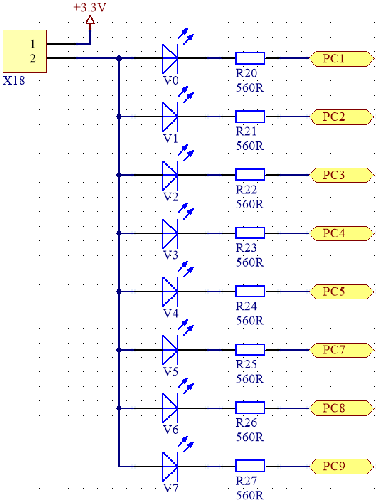
\includegraphics[width=.3\linewidth]{Schuh/Pictures/Basis-leds}}\qquad
    \subfloat[Hardware\label{fig:basisplatine-leds-hard}]{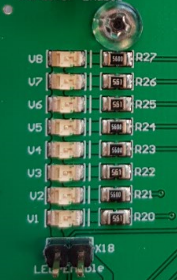
\includegraphics[width=.3\linewidth]{Schuh/Pictures/basis-leds}}\qquad
    \caption[LED-Array der Basisplatine]{LED-Array der \gls{Basisplatine}}
    \label{fig:basisplatine-leds}
\end{figure}

\subsubsection{DIP-Switches}
\label{sec:basis-dip}
Auf der \gls{Basisplatine} wurde ein achtpoliger DIP-Switch realisiert, welcher intern aus acht getrennten Schalten besteht und über die Portleitungen PA0 bis PA3 und PA5 bis PA8 (\fref{fig:basisplatine-dip}) ausgelesen werden kann. Da im Hardwarelayout keine Pullup-Widerstände vorgesehen wurden, muss bei der Programmierung darauf geachtet werden, dass die internen Pullup-Widerstände des Prozessors aktiviert sind. Da jedoch Port Pins PA2 und PA3 mit der UART2-Schnittstelle verbunden sind, erzeugen diese ein Echo, wenn die Schalter S3 und S4 gleichzeitig geschlossen sind. Weiters können durch Jumpern der Stiftleiste X22 (\fref{fig:basisplatine-dip}) alle Schalter im Kippschalter aktiviert oder deaktiviert werden.

\begin{figure}[H]
    \centering
    \subfloat[Schematic\label{fig:basisplatine-dip-schem}]{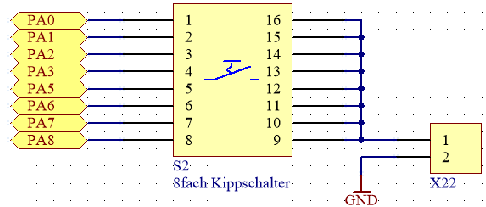
\includegraphics[width=.4\linewidth]{Schuh/Pictures/Basis-dip}}\qquad
    \subfloat[Hardware\label{fig:basisplatine-dip-hard}]{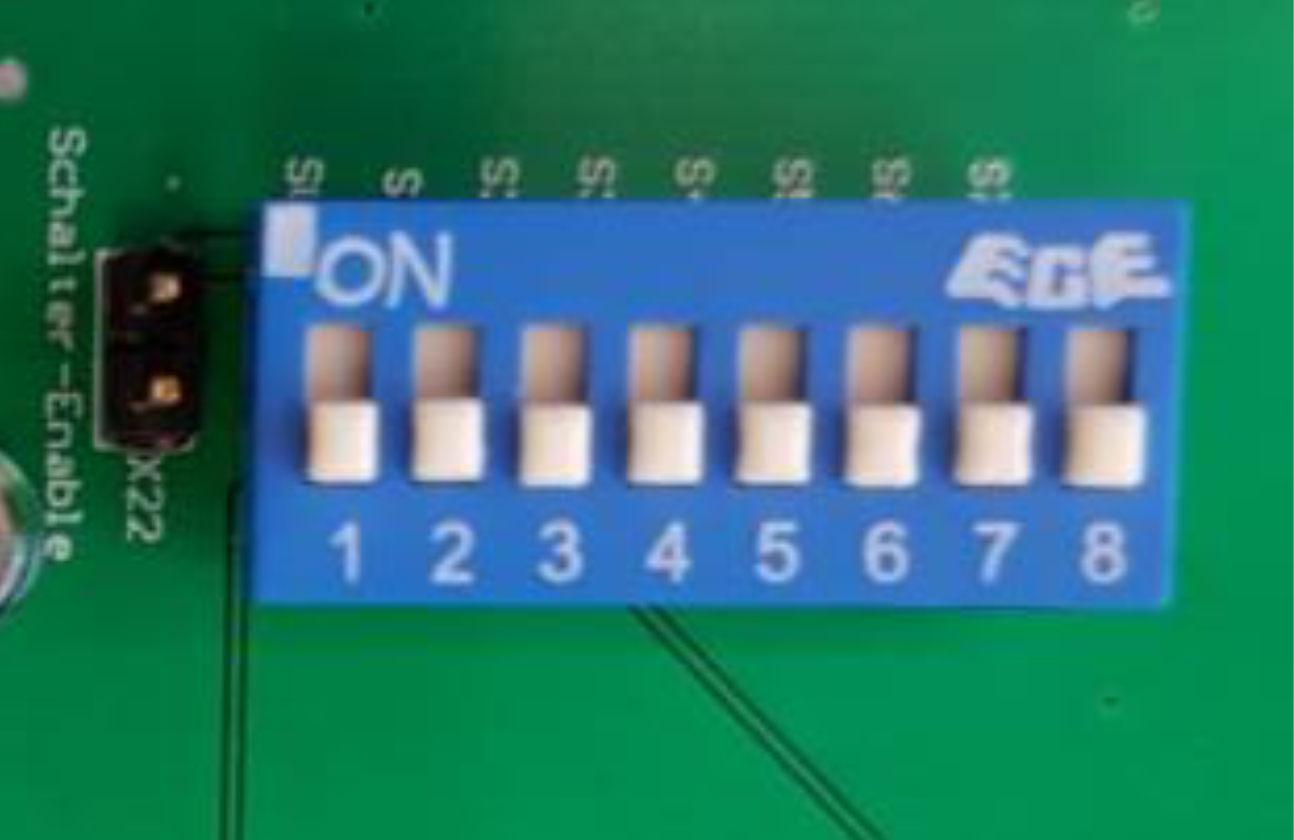
\includegraphics[width=.4\linewidth]{Schuh/Pictures/basis-dip}}\qquad
    \caption[DIP-Switches der Basisplatine]{DIP-Switches der \gls{Basisplatine}}
    \label{fig:basisplatine-dip}
\end{figure}

\subsubsection{USB-Varianten und Versorgung über USB}
Die \gls{Basisplatine} unterstützt hardwaremäßig zwei verschiedene USB-Bauformen und drei verschiedene USB-Funktionen. Diese USB-Funktionen sind USB-Device, USB-Host, USB-OTG (on the go) und werden sowohl von der USB-A Buchse X3 (\fref{fig:basisplatine-usb}), als auch von der USB-B Buchse X1 (\fref{fig:basisplatine-usb}) unterstützt. Da beide Buchsenformen keine ID-Leitung besitzen muss für USB-OTG die dafür benötigte Portleitung PA10 mit einem Pullup-Widerstand versehen werden, um den USB-OTG Modus vorzutäuschen. Weiters müssen für den USB-OTG Modus der Pin1 mit dem Pin2 und der Pin3 mit dem Pin4 auf der zweireihigen Stiftleiste X37 (\fref{fig:basisplatine-usb}) gejumpert werden. Über die Portleitung PA10 kann ausgewählt werden ob der Prozessor als USB-Host oder USB-Device arbeitet. Mit der Portleitung PA9 hingegen kann festgestellt werden ob die Versorgung über die USB Buchse funktioniert.

Falls man im Host-Modus Geräte ohne Adapter anschließen möchte, wurde eine zweite USB Buchse parallel geschaltet. Sollte man die USB-B Buchse auswählen wollen muss man den Pin1 mit dem Pin3 und dem Pin2 mit dem Pin4 auf der zweireihigen Stiftleiste X2 (\fref{fig:basisplatine-usb}) jumpern. Um die USB-A Buchse auswählen muss man den Pin4 mit dem Pin6 und dem Pin3 mit dem Pin5 auf der zweireihigen Stiftleiste X2 (\fref{fig:basisplatine-usb}) jumpern.

Die Feinsicherung F2 (\fref{fig:basisplatine-usb}) dient zur Absicherung des USB-Hosts, welcher die Versorgungsspannung normalerweise zur Verfügung stellt. Laut USB-Spezifikation ist hierbei bei USB 2.0 ein maximaler Strom von \unit{500}{\milli\ampere} erlaubt. Die Sicherung stellt sicher, dass dieser Strom niemals überschritten wird.

Die ESD Protection F1 (\fref{fig:basisplatine-usb}) stellt sicher, dass die Spannungen auf den Datenleitungen zwischen GND und \unit{5}{\volt} bleiben. Durch an- und abstecken an Host-Geräte können Spannungsspitzen auf den Datenleitungen auftreten, die ESD Protection leitet diese ab, sodass der Prozessor nicht beschädigt wird.

\begin{figure}[H]
    \centering
    \subfloat[Schematic\label{fig:basisplatine-usb-schem}]{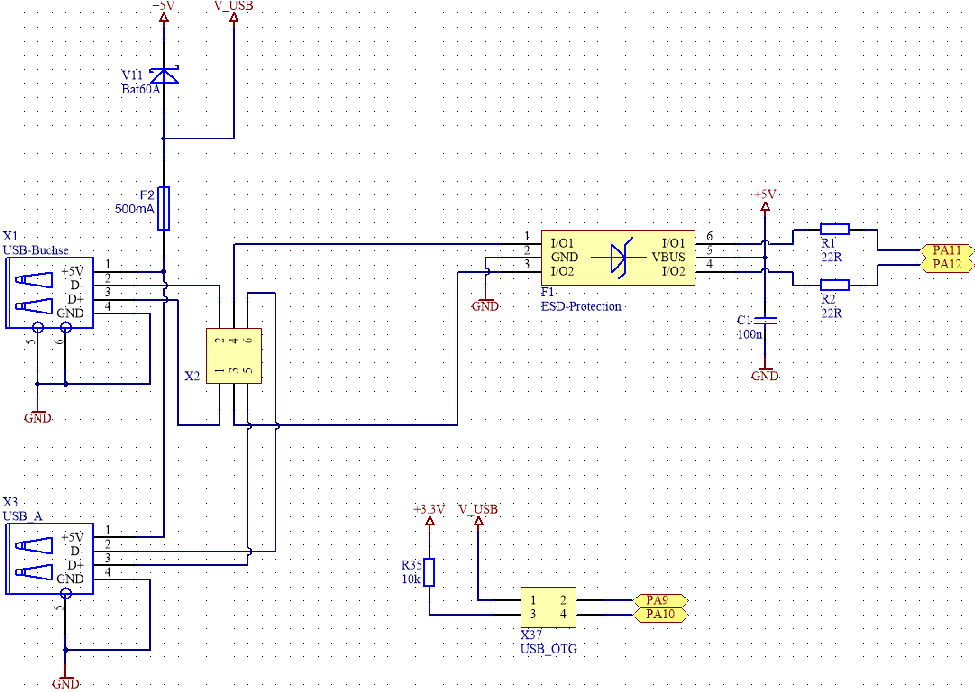
\includegraphics[width=\linewidth]{Schuh/Pictures/Basis-usb}}\qquad
    \subfloat[Hardware\label{fig:basisplatine-usb-hard}]{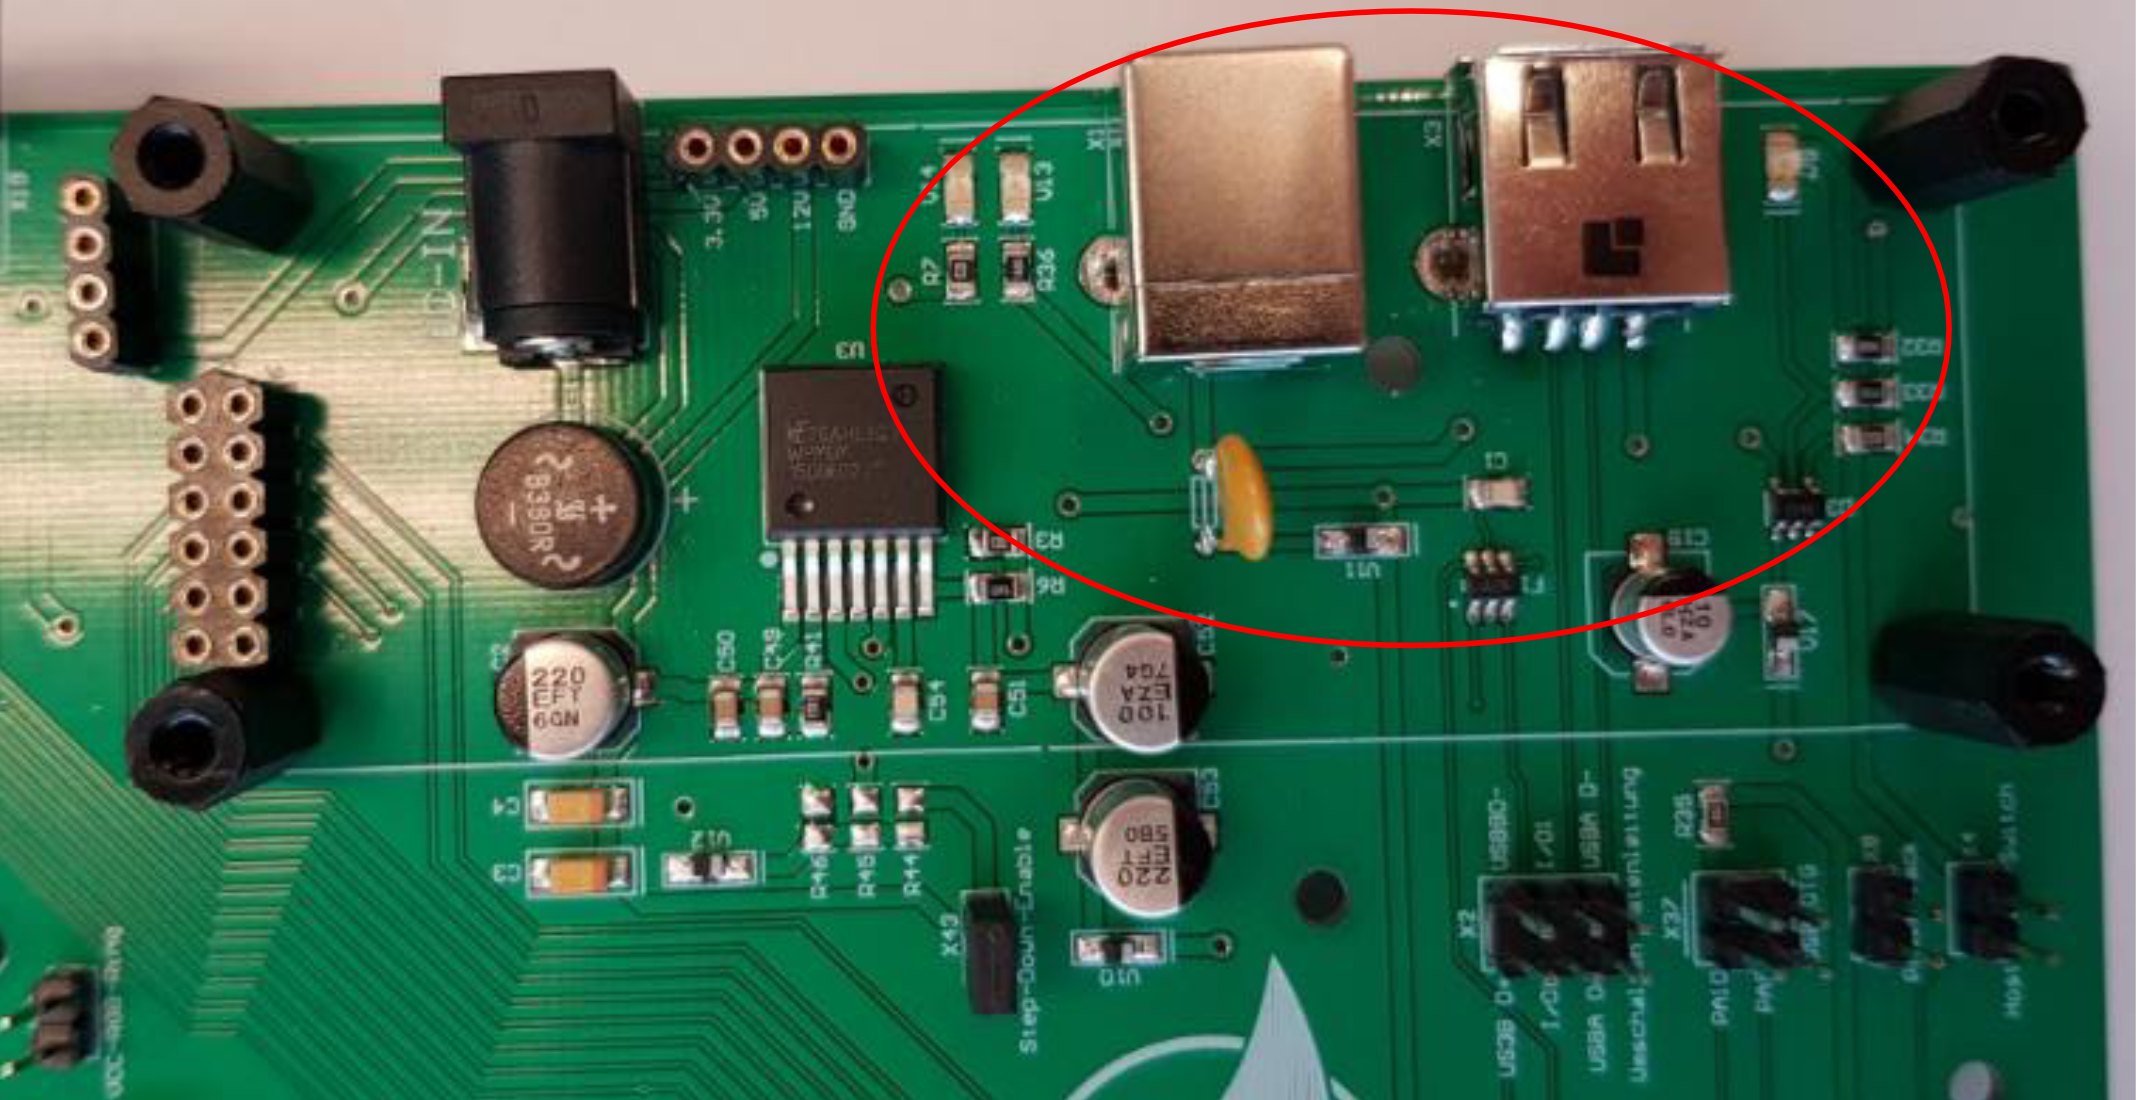
\includegraphics[width=\linewidth]{Schuh/Pictures/basis-usb}}\qquad
    \caption[USB Buchsen der Basisplatine]{USB Buchsen der \gls{Basisplatine}}
    \label{fig:basisplatine-usb}
\end{figure}

\subsubsection{Masseschleife}
Um das Messen mit einem Oszilloskop oder anderen Messgeräten zu vereinfachen wurde eine Masseschleife X5 (\fref{fig:basisplatine-masse}) auf der \gls{Basisplatine} realisiert.

\begin{figure}[H]
    \centering
    \subfloat[Schematic\label{fig:basisplatine-masse-schem}]{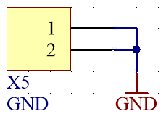
\includegraphics[width=.3\linewidth]{Schuh/Pictures/Basis-masse}}\qquad
    \subfloat[Hardware\label{fig:basisplatine-masse-hard}]{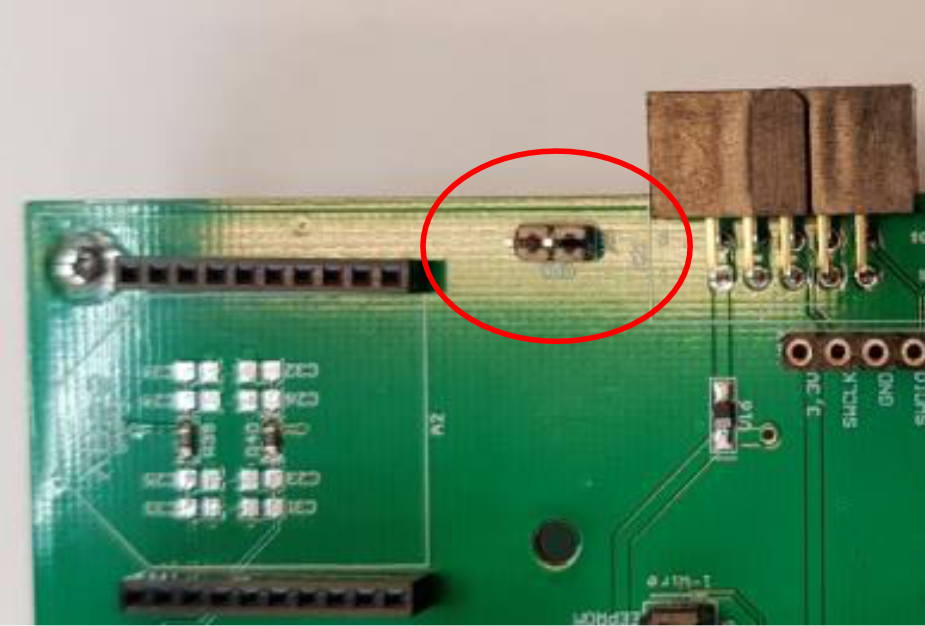
\includegraphics[width=.4\linewidth]{Schuh/Pictures/basis-masse}}\qquad
    \caption[Masseschleife der Basisplatine]{Masseschleife der \gls{Basisplatine}}
    \label{fig:basisplatine-masse}
\end{figure}

\subsubsection{Powerswitch STMPS2141}
Um USB-Geräte zu betreiben, welche selbst keine eigene Spannungsversorgung besitzen (z.B. USB-Sticks) wurde ein Powerswitch D3 (\fref{fig:basisplatine-power}) verbaut. Dieser ermöglicht es die interne \unit{5}{\volt}-Versorgung auf die USB-Buchsen zu legen, damit diese Geräte mit Spannung versorgt werden können. Sollte das Gerät zu viel Strom verbrauchen beginnt die LED V9 (\fref{fig:basisplatine-power}) zu leuchten. Durch Jumpern der Stiftleiste X4 (\fref{fig:basisplatine-power}) an den Port-Pin PC9 kann die Versorgung von externen Geräten gesteuert werden.

\begin{figure}[H]
    \centering
    \subfloat[Schematic\label{fig:basisplatine-power-schem}]{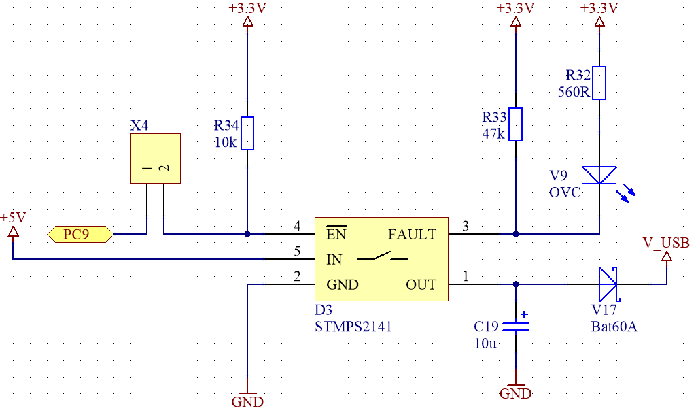
\includegraphics[width=\linewidth]{Schuh/Pictures/Basis-power}}\qquad
    \subfloat[Hardware\label{fig:basisplatine-power-hard}]{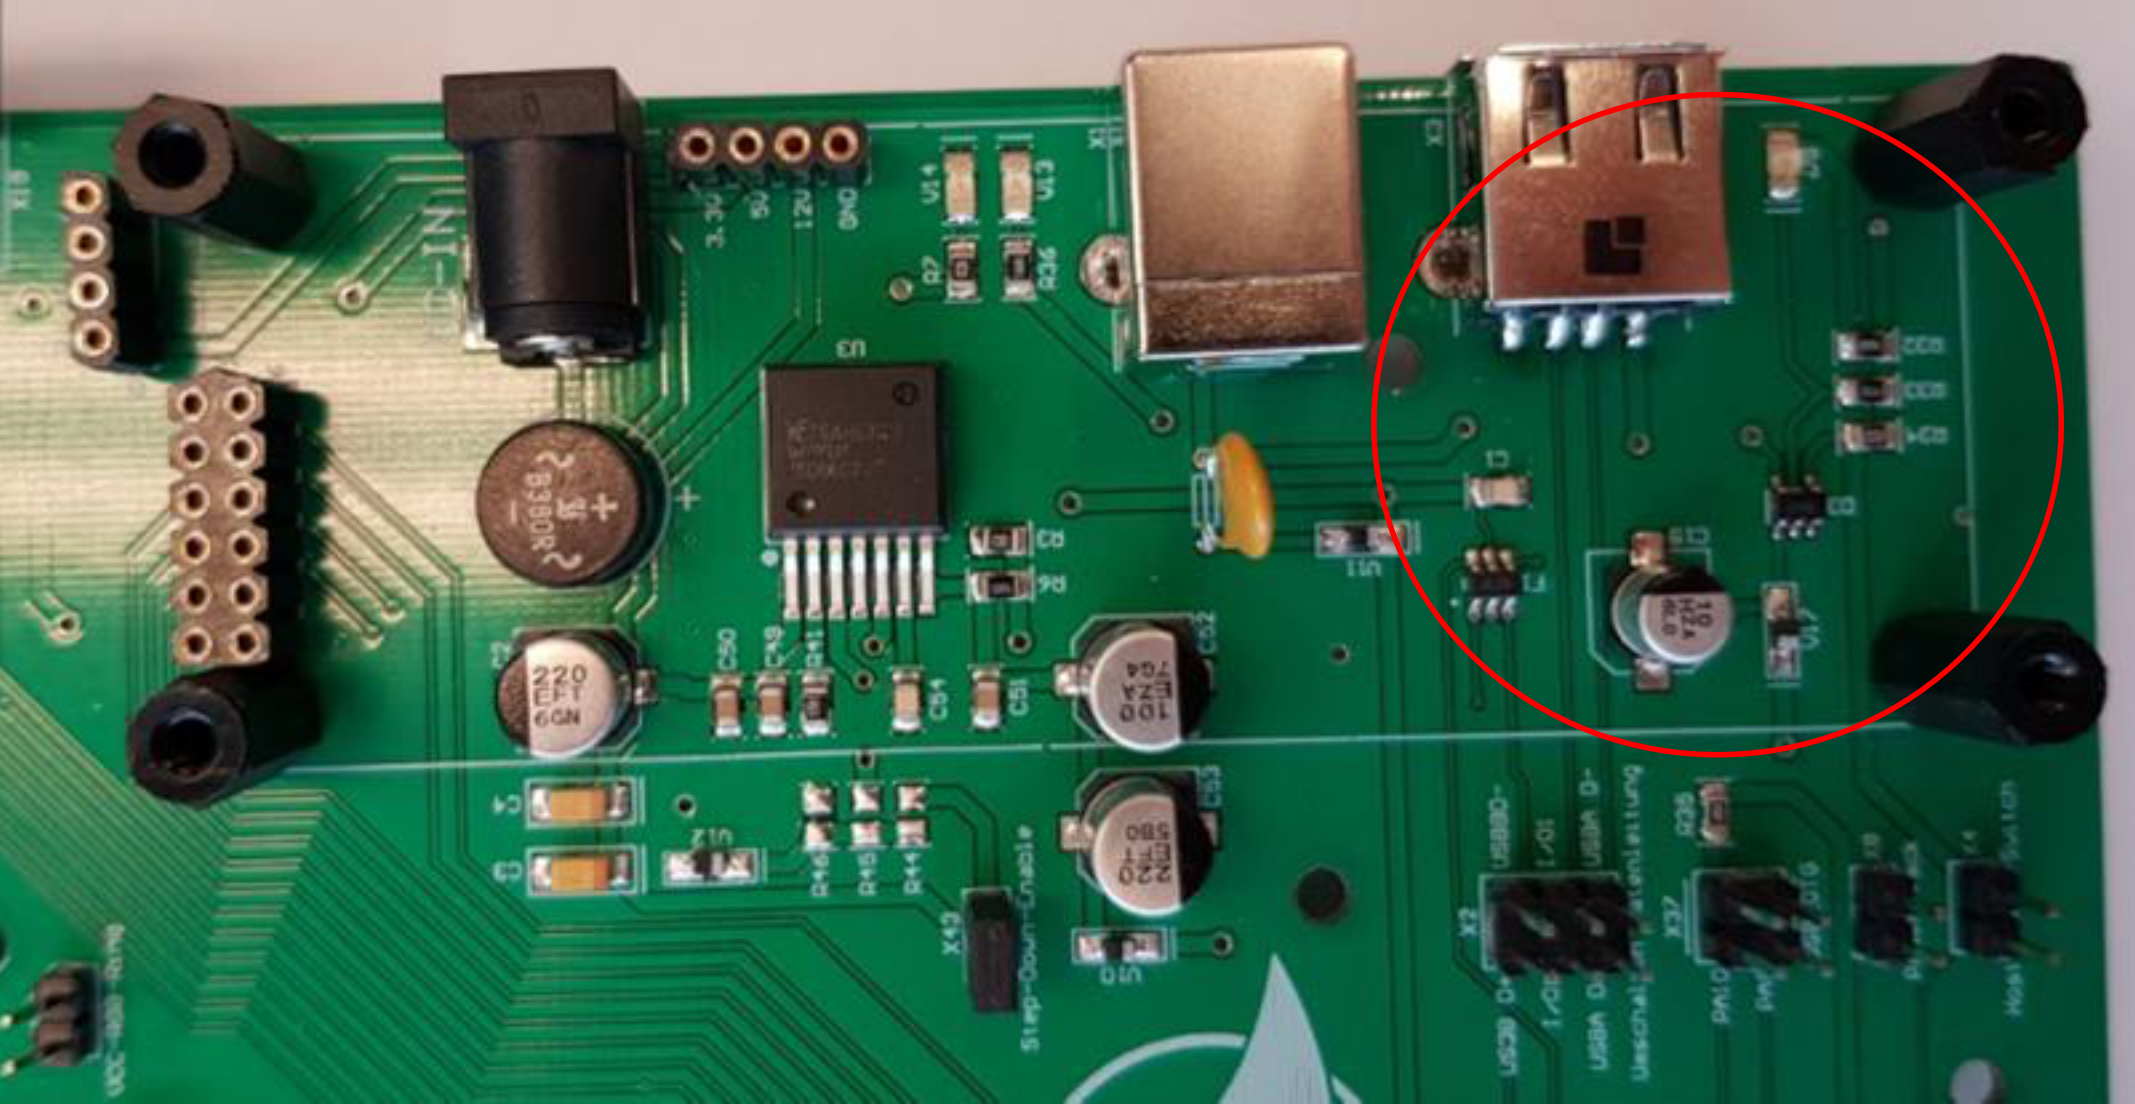
\includegraphics[width=\linewidth]{Schuh/Pictures/basis-power}}\qquad
    \caption[USB Powerswitch der Basisplatine]{USB Powerswitch der \gls{Basisplatine}}
    \label{fig:basisplatine-power}
\end{figure}

\subsubsection{Powerheader}
Um die auf der \gls{Basisplatine} verwendeten Spannungen direkt für Versuchsaufbauten am Steckbrett oder für externe Sensoren verwenden zu können wurden zwei Buchsenleisten X6 und X7 (\fref{fig:basisplatine-pwrhdr}) ausgeführt, welche diese Spannungen bereitstellen. Dabei ist zu beachten, dass am \unit{12}{\volt}-Ausgang nur \unit{+12}{\volt} anliegen, wenn die Basisplatine über ein externes Netzteil mit einer Ausgangsspannung von \unit{+12}{\volt} betrieben wird. Sollte eine geringere Spannung über das Netzgerät eingespeist werden liegt diese am Ausgang an, wenn hingegen kein Netzteil verwendet wird ist dieser Ausgang spannungsfrei.

\begin{figure}[H]
    \centering
    \subfloat[Schematic\label{fig:basisplatine-pwrhdr-schem}]{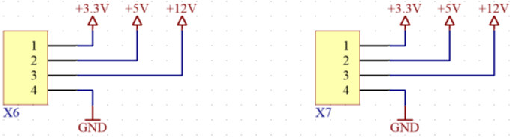
\includegraphics[width=\linewidth]{Schuh/Pictures/Basis-pwrhdr}}\qquad
    \subfloat[Hardware\label{fig:basisplatine-pwrhdr-hard}]{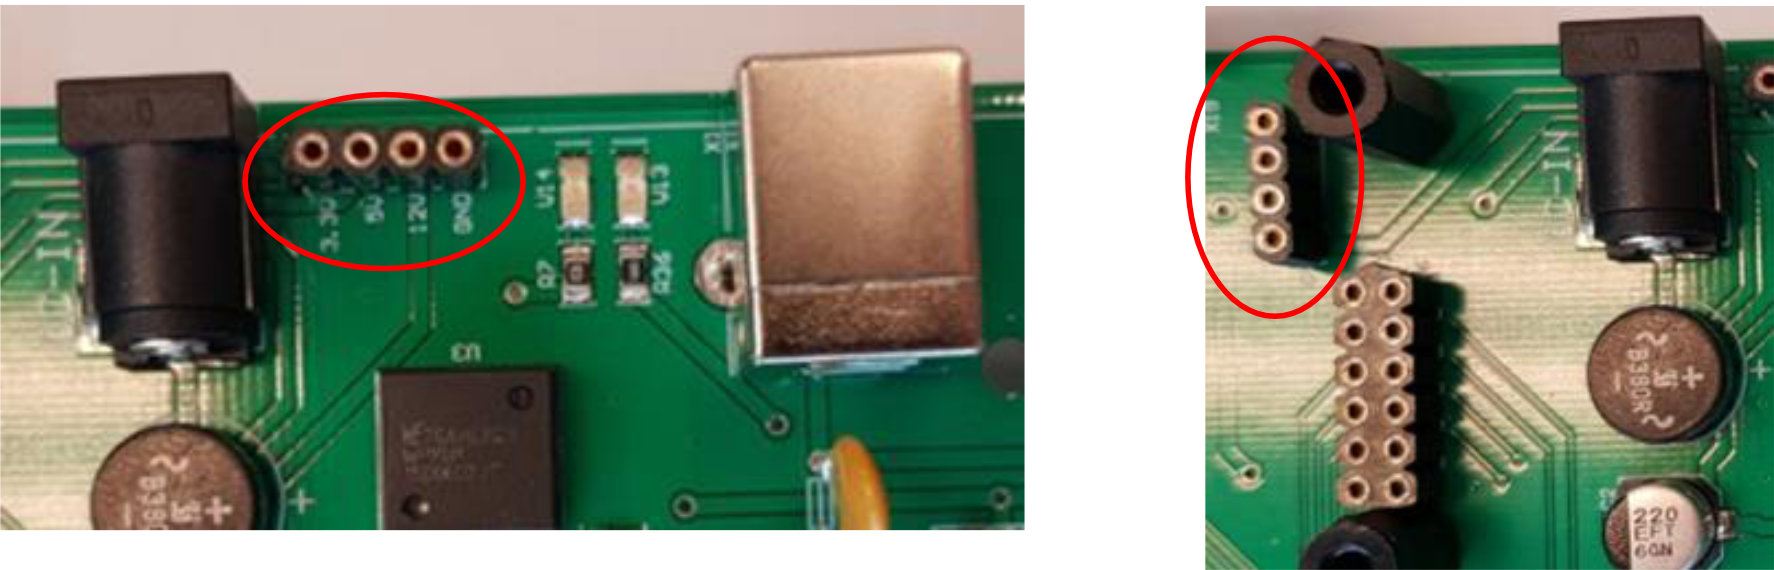
\includegraphics[width=\linewidth]{Schuh/Pictures/basis-pwrhdr}}\qquad
    \caption[Powerheader der Basisplatine]{Powerheader der \gls{Basisplatine}}
    \label{fig:basisplatine-pwrhdr}
\end{figure}

\subsubsection{3,3 V-Versorgung}
Zur Überprüfung ob die \gls{Basisplatine} mit der Betriebsspannung von \unit{+3,3}{\volt} über das \gls{Core-Modul} versorgt wird, wurde die LED V14 (\fref{fig:basisplatine-3v3}) zur optischen Kontrolle eingebaut. Wenn die Basisplatine mit Spannung versorgt wird, beginnt diese zu leuchten.

\begin{figure}[H]
    \centering
    \subfloat[Schematic\label{fig:basisplatine-3v3-schem}]{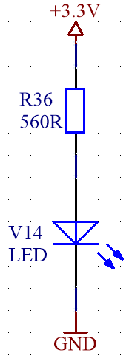
\includegraphics[width=.2\linewidth]{Schuh/Pictures/Basis-3v3}}\qquad
    \subfloat[Hardware\label{fig:basisplatine-3v3-hard}]{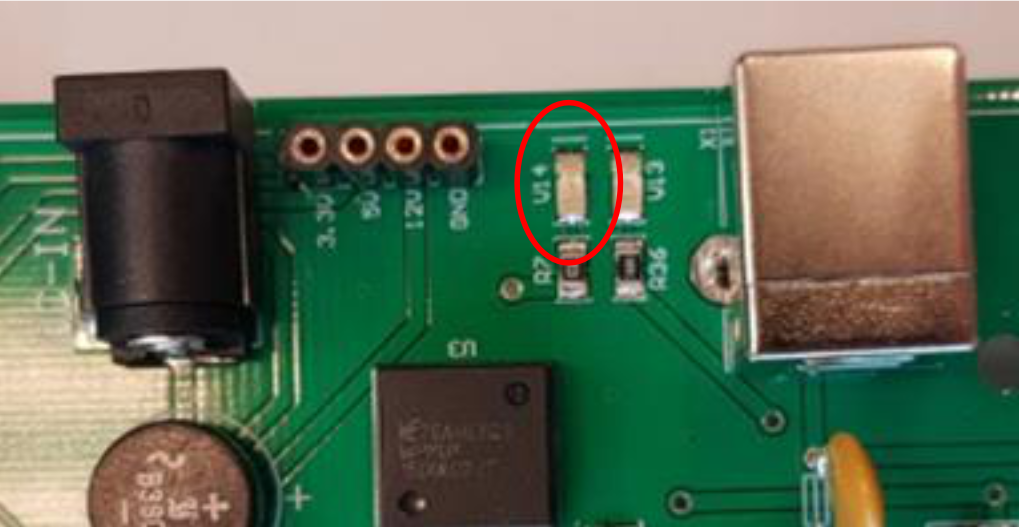
\includegraphics[width=.4\linewidth]{Schuh/Pictures/basis-3v3}}\qquad
    \caption[\unit{3,3}{\volt}-Versorgung der Basisplatine]{\unit{3,3}{\volt}-Versorgung der \gls{Basisplatine}}
    \label{fig:basisplatine-3v3}
\end{figure}

\subsubsection{Spannungsversorgung über DC-Buchse}
Als weitere Spannungsversorgungsmöglichkeit bietet die \gls{Basisplatine} die Möglichkeit ein \unit{9}{\volt} bis \unit{12}{\volt} DC-Netzteil am die DC-Buchse J1 (\fref{fig:basisplatine-dc}) anzuschließen um die Basisplatine mit Spannung zu versorgen. Der Brückengleichrichter U1 (\fref{fig:basisplatine-dc}) dient dabei lediglich als Verpolungsschutz und nicht als Gleichrichter für Wechselspannung. Das Anlegen von Wechselspannung an die DC-Buchse J1 (\fref{fig:basisplatine-dc}) sollte aus Sicherheitsgründen unterlassen werden. Um aus der hohen Spannung, welche von der DC-Buchse kommt, die Betriebsspannung von \unit{+5}{\volt} zu generieren wurde ein Step-Down Modul U3 (\fref{fig:basisplatine-dc}) der Firma Würth verbaut. Zur Überprüfung ob das Step-Down Modul die Betriebsspannung von \unit{+5}{\volt} generiert, wurde die LED V13 (\fref{fig:basisplatine-dc}) zur optischen Kontrolle eingebaut. Wenn das Step-Down Modul die gewünschte Spannung generiert, beginnt diese zu leuchten. Die Stiftleiste X43 (\fref{fig:basisplatine-dc}) kann im Bedarfsfall gejumpert werden, wenn ein Unterspannungsschutz der Versorgungsspannung gewünscht ist. Um die vom Step-Down Modul generierte Spannung verwenden zu können muss lediglich die Stiftleiste X8 (\fref{fig:basisplatine-dc}) mit einem Jumper versehen werden.

\begin{figure}[H]
    \centering
    \subfloat[Schematic\label{fig:basisplatine-dc-schem}]{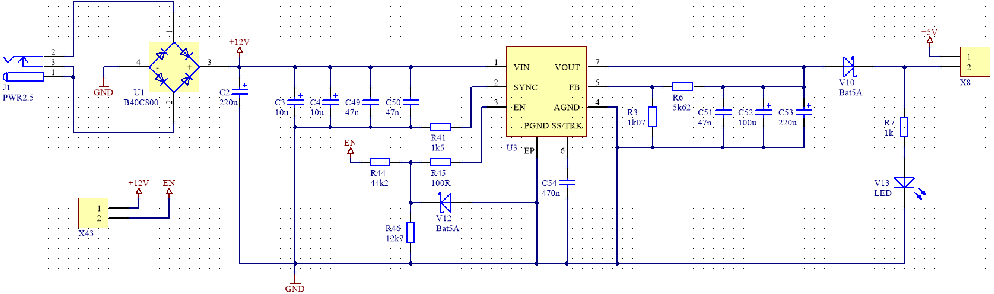
\includegraphics[width=\linewidth]{Schuh/Pictures/Basis-dc}}\qquad
    \subfloat[Hardware\label{fig:basisplatine-dc-hard}]{\includegraphics[width=\linewidth]{Schuh/Pictures/basis-dc}}\qquad
    \caption[DC-Versorgung der Basisplatine]{DC-Versorgung der \gls{Basisplatine}}
    \label{fig:basisplatine-dc}
\end{figure}

\subsubsection{RGB-LED Ring \cite{basis:ws2812b}}
Auf der \gls{Basisplatine} wurde ein aus zwölf RGB-LEDs bestehender Ring aufgebaut, welcher in den verschiedensten Farben leuchten kann. Jede RGB-LED besitzt einen eigenen eingebauten Controller. Die Ansteuerung der LEDs wird über den Port-Pin PB0 realisiert. Um diesen verwenden zu können muss zuvor die Stiftleiste X41 (\fref{fig:basisplatine-ledring}) mit einem Jumper versehen werden. Weiters muss die Spannungsversorgung der LEDs gewährleistet sein. Dazu muss lediglich die Stiftleiste X42 (\fref{fig:basisplatine-ledring}) mit einem Jumper versehen werden.

\begin{figure}[H]
    \centering
    \subfloat[Schematic\label{fig:basisplatine-ledring-schem}]{\includegraphics[width=.75\linewidth]{Schuh/Pictures/Basis-ledring}}\qquad
    \subfloat[Hardware\label{fig:basisplatine-ledring-hard}]{\includegraphics[width=.3\linewidth]{Schuh/Pictures/basis-ledring}}\qquad
    \caption[RGB-LED Ring der Basisplatine]{RGB-LED Ring der \gls{Basisplatine}}
    \label{fig:basisplatine-ledring}
\end{figure}

Zur Programmierung der LEDs muss über den Port PB0 ein Datenwort übetragen werden, welches 24 bit pro LED enthält, siehe \fref{fig:basisplatine-ledring-data}. Dies ergibt insgesamt 288 bit, welche übertragen werden müssen. Wie die Übertragung genau aussieht kann aus \fref{fig:basisplatine-ledring-timing} entnommen werden.

\fig{basisplatine-ledring-data}{RGB-LED Ring Datenstruktur}{RGB-LED Ring Datenstruktur \cite{basis:ws2812b}}{\textwidth}{Schuh/Pictures/Basis-ledring-data}
\fig{basisplatine-ledring-timing}{RGB-LED Ring Timing Diagram}{RGB-LED Ring Timing Diagram \cite{basis:ws2812b}}{\textwidth}{Schuh/Pictures/Basis-ledring-timing}

Die Daten für jede LED im Ring werden seriell hintereinander wie in \fref{fig:basisplatine-ledring-data} beschrieben übertragen, hierbei wird zuerste die erste LED angesprochen, wenn diese die richtigen Daten hat, leitet sie alle weiteren Datenpakete transparent weiter, sodass danach die zweite LED angesprochen wird und so weiter, bis ein Reset Code (\unit{50}{\micro\second} oder länger \enquote{High}) gesendet wird. Danach kann wieder die erste LED angesprochen werden. das genau Timing kann hierbai aus dem Datenblatt \cite{basis:ws2812b} entnommen werden.

\subsubsection{Sensor-Selektion}
Da der verbaute Prozessor zu wenig Portleitungen besitzt um alle Sensoren und Module mit einer eigenen Portleitung zu versorgen, werden einige Portleitungen mehrmals verwendet. Um nun einzelne Module oder Sensoren verwenden zu können, müssen diese einsprechend gejumpert werden. Eine dieser Stiftleisten ist der Header X9 (\fref{fig:basisplatine-ssel}), welches es ermöglicht zwischen einem Potentiometer (\gls{ADC}), Piezo-Summer, einem LFU, einem Infrarotempfänger, einem Temperaturfühler und einem NE555 auszuwählen.

Eine weitere dieser Stiftleisten ist der Header X11 (\fref{fig:basisplatine-ssel2}), welche es ermöglicht zwischen dem Beschleunigungssensor und dem EEPROM auszuwählen.

\begin{figure}[H]
    \centering
    \subfloat[Schematic\label{fig:basisplatine-ssel-schem}]{\includegraphics[width=.5\linewidth]{Schuh/Pictures/Basis-ssel}}\qquad
    \subfloat[Hardware\label{fig:basisplatine-ssel-hard}]{\includegraphics[width=.3\linewidth]{Schuh/Pictures/basis-ssel}}\qquad
    \caption[Sensor-Selektion der Basisplatine]{Sensor-Selektion der \gls{Basisplatine}}
    \label{fig:basisplatine-ssel}
\end{figure}

\begin{figure}[H]
    \centering
    \subfloat[Schematic\label{fig:basisplatine-ssel2-schem}]{\includegraphics[width=.5\linewidth]{Schuh/Pictures/Basis-ssel2}}\qquad
    \subfloat[Hardware\label{fig:basisplatine-ssel2-hard}]{\includegraphics[width=.3\linewidth]{Schuh/Pictures/basis-ssel2}}\qquad
    \caption[Sensor-Selektion der Basisplatine]{Sensor-Selektion der \gls{Basisplatine}}
    \label{fig:basisplatine-ssel2}
\end{figure}

\subsubsection{Piezo-Summer}
Auf der \gls{Basisplatine} wurde ein Piezo-Summer B4 (\fref{fig:basisplatine-piezo}) verbaut, welcher über den Port-Pin PB0 angesteuert werden kann. Ja nach anliegender Taktfrequenz am Eingang des Summers wird der erzeugte Ton höher oder tiefer. Um den Piezo-Summer verwenden zu können muss lediglich der Pin11 mit dem Pin12, der zweireihige Stiftleiste X9 (\fref{fig:basisplatine-ssel}), gejumpert werden.

\begin{figure}[H]
    \centering
    \subfloat[Schematic\label{fig:basisplatine-piezo-schem}]{\includegraphics[width=.5\linewidth]{Schuh/Pictures/Basis-piezo}}\qquad
    \subfloat[Hardware\label{fig:basisplatine-piezo-hard}]{\includegraphics[width=.3\linewidth]{Schuh/Pictures/basis-piezo}}\qquad
    \caption[Piezo-Summer der Basisplatine]{Piezo-Summer der \gls{Basisplatine}}
    \label{fig:basisplatine-piezo}
\end{figure}

\subsubsection{Potentiometer}
Es wurden zwei Potentiometer R9 und R4 hardwaremäßig auf der \gls{Basisplatine} vorgesehen. Diese sind direkt mit einem \gls{ADC}-Eingang des Prozessors verbunden. Der Unterschied zwischen den Potentiometern R9 und R4 besteht darin, dass das Potentiometer R4 über einen Jumper auf der Stiftleiste X40 (\fref{fig:basisplatine-poti2-schem}) aktiviert werden muss und dieses an einem anderen Port-Pin angeschlossen ist. Dieser Aufbau wurde deswegen gewählt da damit, damit an den \gls{ADC}-Eingang auch optional ein anderes Signal angelegt werden kann. 

\begin{figure}[H]
    \centering
    \subfloat[Schematic\label{fig:basisplatine-poti1-schem}]{\includegraphics[width=.4\linewidth]{Schuh/Pictures/Basis-poti1}}\qquad
    \subfloat[Schematic\label{fig:basisplatine-poti2-schem}]{\includegraphics[width=.4\linewidth]{Schuh/Pictures/Basis-poti2}}\qquad
    \subfloat[Hardware\label{fig:basisplatine-poti-hard}]{\includegraphics[width=.4\linewidth]{Schuh/Pictures/basis-poti}}\qquad
    \caption[Potentiometer der Basisplatine]{Potentiometer der \gls{Basisplatine}}
    \label{fig:basisplatine-poti}
\end{figure}

\subsubsection{EEPROM}
Um Daten permanent speichern zu können wurde das EEPROM D1 (\fref{fig:basisplatine-eeprom}) vorgesehen. Standardmäßig wird das EEPROM 24AA256 verwendet, welches es ermöglicht 256 kbit abzuspeichern. Dieses EEPROM besitzt eine Write-Protection WP welche es ermöglicht das EEPROM schreibgeschützt zu schalten. Die Write-Protection kann über die Portleitung PB5 gesteuert werden. Damit das Signal am EEPROM ankommt, muss jedoch der Pin3 mit dem Pin4 der zweireihigen Stiftleiste X11 (\fref{fig:basisplatine-ssel2}) gejumpert werden. Die Kommunikation mit dem EEPROM erfolgt über den \IIC{}-Bus (Adresse \texttt{0xA0}).

\begin{figure}[H]
    \centering
    \subfloat[Schematic\label{fig:basisplatine-eeprom-schem}]{\includegraphics[width=.5\linewidth]{Schuh/Pictures/Basis-eeprom}}\qquad
    \subfloat[Hardware\label{fig:basisplatine-eeprom-hard}]{\includegraphics[width=.3\linewidth]{Schuh/Pictures/basis-eeprom}}\qquad
    \caption[EEPROM der Basisplatine]{EEPROM der \gls{Basisplatine}}
    \label{fig:basisplatine-eeprom}
\end{figure}

\subsubsection{Beschleunigungssensor}
Auf der \gls{Basisplatine} wurde auch ein Beschleunigungssensormodul mit dem Beschleunigungssensor BMA020 vorgesehen. Die Kommunikation mit dem Beschleunigungssensor erfolgt mit Hilfe des \IIC{}-Buses (Adresse \texttt{0x70}). Durch diesen Sensor kann die Neigung, sowie die Kraft welche auf die Platine wirkt in der X, Y und Z-Richtung erfasst werden. Der Beschleunigungssensor besitzt einen Interrupt-Pin, welcher es ermöglicht ein Interrupt auszulösen. Der Interrupt kann über die Portleitung PB5 empfangen werden. Damit das Interrupt-Signal an der Portleitung PB5 ankommt, muss jedoch der Pin1 mit dem Pin2 der zweireihigen Stiftleiste X11 (\fref{fig:basisplatine-ssel2}) gejumpert werden.

\begin{figure}[H]
    \centering
    \subfloat[Schematic\label{fig:basisplatine-bma-schem}]{\includegraphics[width=.5\linewidth]{Schuh/Pictures/Basis-bma}}\qquad
    \subfloat[Hardware\label{fig:basisplatine-bma-hard}]{\includegraphics[width=.3\linewidth]{Schuh/Pictures/basis-bma}}\qquad
    \caption[Beschleunigungssensor der Basisplatine]{Beschleunigungssensor der \gls{Basisplatine}}
    \label{fig:basisplatine-bma}
\end{figure}

\subsubsection{IR-Receiver}
Um die Platine auch mit einer Fernbedienung oder einem Mobiltelefon steuern zu können würde ein IR-Receiver verbaut. Dieser Sensor wurde hardwaremäßig unter dem NEXTION-Display angebracht. Der IR-Receiver arbeitet mit einer Wellenlänge von 850nm bis 1000nm und einer Trägerfrequenz von 38kHz. Das vom IR-Receiver empfangene Signal wird direkt im Receiver demoduliert und anschließend zur Stiftleiste X9 (\fref{fig:basisplatine-ssel}) weitergeleitet. Um den IR-Receiver verwenden zu können muss lediglich der Pin7 mit dem Pin8, der Stiftleiste X9 (\fref{fig:basisplatine-ssel}), gejumpert werden.

\begin{figure}[H]
    \centering
    \subfloat[Schematic\label{fig:basisplatine-ir-schem}]{\includegraphics[width=.5\linewidth]{Schuh/Pictures/Basis-ir}}\qquad
    \subfloat[Hardware\label{fig:basisplatine-ir-hard}]{\includegraphics[width=.3\linewidth]{Schuh/Pictures/basis-ir}}\qquad
    \caption[IR-Receiver der Basisplatine]{IR-Receiver der \gls{Basisplatine}}
    \label{fig:basisplatine-ir}
\end{figure}

\subsubsection{Temperatursensor}
Um die Umgebungstemperatur feststellen zu können wurde auf der Basisplatine der Temperaturfühler DS18B20 verbaut, welcher mit Hilfe des 1-Wire Protokolls angesprochen werden kann. Die maximale Mesfehler dieses Temperatursensors beträgt ±0,5°C laut Datenblattangabe. Um den Temperaturfühler verwenden zu können muss lediglich der Pin9 mit dem Pin10, der Stiftleiste X9 (\fref{fig:basisplatine-ssel}), gejumpert werden. 

\begin{figure}[H]
    \centering
    \subfloat[Schematic\label{fig:basisplatine-temp-schem}]{\includegraphics[width=.5\linewidth]{Schuh/Pictures/Basis-temp}}\qquad
    \subfloat[Hardware\label{fig:basisplatine-temp-hard}]{\includegraphics[width=.3\linewidth]{Schuh/Pictures/basis-temp}}\qquad
    \caption[Temperatursensor der Basisplatine]{Temperatursensor der \gls{Basisplatine}}
    \label{fig:basisplatine-temp}
\end{figure}

\subsubsection{Lichtwandler LFU}
Der auf der \gls{Basisplatine} realisierte LFU (Licht-Frequenz-Wandler), wandeltet wie der Name bereits sagt Licht in eine bestimmte Frequenz um. Je höher die Bestrahlungsstärke des Lichts, desto höher wird die über den Output des LFUs ausgegebene Frequenz. Den linearen Zusammenhang zwischen der Bestrahlungsstärke und der ausgegebenen Frequenz kann aus \fref{fig:basisplatine-lfu-freq} entnommen werden. Um den LFU verwenden zu können muss lediglich der Pin5 mit dem Pin6, der Stiftleiste X9 (\fref{fig:basisplatine-ssel}), gejumpert werden.

\begin{figure}[H]
    \centering
    \subfloat[Schematic\label{fig:basisplatine-lfu-schem}]{\includegraphics[width=.5\linewidth]{Schuh/Pictures/Basis-lfu}}\qquad
    \subfloat[Hardware\label{fig:basisplatine-lfu-hard}]{\includegraphics[width=.3\linewidth]{Schuh/Pictures/basis-lfu}}\qquad
    \caption[LFU der Basisplatine]{LFU der \gls{Basisplatine}}
    \label{fig:basisplatine-lfu}
\end{figure}
\fig{basisplatine-lfu-freq}{Frequenzgang des LFUs}{Frequenzgang des LFUs}{0.5\textwidth}{Schuh/Pictures/Basis-lfu-freq}

\subsubsection{RGB-LED}
Auf der \gls{Basisplatine} wurde ebenso eine RGB-LED \cite{basis:rgbled} verbaut, welche mit Hilfe des LED-Drivers D4 (\fref{fig:basisplatine-rgbled}) \cite{basis:rgbdriver}, welcher mit dem \IIC{}-Bus (Adresse \texttt{0x70}) angesteuert werden kann. Dieser LED-Driver hat den Vorteil, dass er eine interne Stromüberwachung besitzt. Dadurch benötigen die einzelnen Anoden der RGB-LED keine Vorwiderstände, da sich der Strom automatisch entsprechend der gewünschten Farbe reguliert.

\begin{figure}[H]
    \centering
    \subfloat[Schematic\label{fig:basisplatine-rgbled-schem}]{\includegraphics[width=.5\linewidth]{Schuh/Pictures/Basis-rgbled}}\qquad
    \subfloat[Hardware\label{fig:basisplatine-rgbled-hard}]{\includegraphics[width=.3\linewidth]{Schuh/Pictures/basis-rgbled}}\qquad
    \caption[RGB-LED der Basisplatine]{RGB-LED der \gls{Basisplatine}}
    \label{fig:basisplatine-rgbled}
\end{figure}
\fig{basisplatine-rgbled-befehl}{Befehlsaufbau der RGB-LED}{Befehlsaufbau der RGB-LED \cite{basis:rgbdriver}}{\textwidth}{Schuh/Pictures/Basis-rgbled-befehl}
\fig{basisplatine-rgbled-register}{Register der RGB-LED}{Register der RGB-LED \cite{basis:rgbdriver}}{\textwidth}{Schuh/Pictures/Basis-rgbled-register}
\fig{basisplatine-rgbled-seq}{Sequenzen der RGB-LED}{Sequenzen der RGB-LED \cite{basis:rgbdriver}}{\textwidth}{Schuh/Pictures/Basis-rgbled-seq}

\subsubsection{Arduino-Shield-Header}
Um Hardware des Arduino-Mikrocontrollersystems nutzten zu können, ohne selbst großen Aufwand in die Entwicklung entsprechender Module investieren zu müssen, wurde ein Arduino-Shield-Header auf der \gls{Basisplatine} vorgesehen. Dieser ermöglicht es durch die Portkompatibilität mit einem Arduino, dessen Shields zu verwenden oder selbst Shields entwickeln zu können. Möchte man nun ein Arduino-Shield verwenden muss dieses lediglich in die vorgesehene Buchsenleiste X33 (\fref{fig:basisplatine-arduino}) gesteckt werden. Da jedes Arduino-Shield die Möglichkeit besitzt eine Referenzspannung für diverse ADCs zu vergeben wurde das Potentiometer R31 vorgesehen, um diesen Spannungspegel variabel zu gestallten. Darüber hinaus gibt es noch die Möglichkeit bei speziellen Shields zu definieren mit welcher Betriebsspannung die darüberliegenden versorgt werden sollen. Dazu wurde die Stiftleiste X27 verbaut, um festzulegen ob die darüberliegenden Shields mit \unit{+5}{\volt} oder \unit{+3,3}{\volt} versorgt werden. Sollte kein Jumper gesetzt werden wird automatisch auf die \unit{+5}{\volt} Spannungsversorgung zurückgegriffen.

\begin{figure}[H]
    \centering
    \subfloat[Schematic\label{fig:basisplatine-arduino-schem}]{\includegraphics[width=.5\linewidth]{Schuh/Pictures/Basis-arduino}}\qquad
    \subfloat[Hardware\label{fig:basisplatine-arduino-hard}]{\includegraphics[width=.3\linewidth]{Schuh/Pictures/basis-arduino}}\qquad
    \caption[Arduino-Shield-Header der Basisplatine]{Arduino-Shield-Header der \gls{Basisplatine}}
    \label{fig:basisplatine-arduino}
\end{figure}

\subsubsection{WLAN-Modul \cite{basis:wlan}}
Um Daten ohne großen Aufwand direkt in das Heimnetzwerk einspeisen zu können, wurde auf der auf der \gls{Basisplatine} ein Steckplatz X35 (\fref{fig:basisplatine-wlan}) für ein ESP8266 W-LAN Modul vorgesehen. Dieses Funkmodul benutzt zu Kommunikation mit dem Prozessor des Core-Moduls die UART2 Schnittstelle und sendet die Daten mit einer Sendefrequenz von \unit{2,4}{\giga\hertz} im ISM-Band. Wenn man die Firmware des ESP8266 verändern möchte muss man lediglich die Portleitung GPIO0 des ESP8266, durch jumpern von Pin2 und Pin3 der Stiftleiste X39 (\fref{fig:basisplatine-wlan}), gegen Masse schalten.

\begin{figure}[H]
    \centering
    \subfloat[Schematic\label{fig:basisplatine-wlan-schem}]{\includegraphics[width=.5\linewidth]{Schuh/Pictures/Basis-wlan}}\qquad
    \subfloat[Hardware\label{fig:basisplatine-wlan-hard}]{\includegraphics[width=.3\linewidth]{Schuh/Pictures/basis-wlan}}\qquad
    \caption[WLAN-Modul der Basisplatine]{WLAN-Modul der \gls{Basisplatine}}
    \label{fig:basisplatine-wlan}
\end{figure}

\subsubsection{XBee-Pro-Modul}
Um Daten ohne großen Aufwand per Funk übertragen können, wurde auf der auf der \gls{Basisplatine} ein Steckplatz A2 (\fref{fig:basisplatine-xbee}) für ein XBee-Pro Modul vorgesehen. Dieses Funkmodul benutzt zu Kommunikation mit dem Prozessor des \gls{Core-Modul}s die UART2 Schnittstelle und sendet die Daten mit einer Sendefrequenz von \unit{2,4}{\giga\hertz} im ISM-Band. Darüber hinaus weist das Funkmodul eine maximale Datenübertragungsrate von 250 kb/s auf und hat eine maximale Reichweite von \unit{1600}{\metre}.

\begin{figure}[H]
    \centering
    \subfloat[Schematic\label{fig:basisplatine-xbee-schem}]{\includegraphics[width=.5\linewidth]{Schuh/Pictures/Basis-xbee}}\qquad
    \subfloat[Hardware\label{fig:basisplatine-xbee-hard}]{\includegraphics[width=.3\linewidth]{Schuh/Pictures/basis-xbee}}\qquad
    \caption[XBee-Pro-Modul der Basisplatine]{XBee-Pro-Modul der \gls{Basisplatine}}
    \label{fig:basisplatine-xbee}
\end{figure}

\subsubsection{HC-06-Modul \cite{basis:hc06}}
Um Daten ohne großen Aufwand per Bluetooth übertragen können, wurde auf der auf der \gls{Basisplatine} ein Steckplatz X28 (\fref{fig:basisplatine-hc06}) für ein HC-06 Bluetooth-Modul vorgesehen. Dieses Bluetooth-Modul benutzt zur Kommunikation mit dem Prozessor des \gls{Core-Modul}s die UART1 Schnittstelle und sendet die Daten mit einer Sendefrequenz von \unit{2,4}{\giga\hertz} im ISM-Band. Darüber hinaus weist das Bluetooth-Modul eine maximale Datenübertragungsrate von 1382400 baud auf.

\begin{figure}[H]
    \centering
    \subfloat[Schematic\label{fig:basisplatine-hc06-schem}]{\includegraphics[width=.5\linewidth]{Schuh/Pictures/Basis-hc06}}\qquad
    \subfloat[Hardware\label{fig:basisplatine-hc06-hard}]{\includegraphics[width=.3\linewidth]{Schuh/Pictures/basis-hc06}}\qquad
    \caption[HC-06-Modul der Basisplatine]{HC-06-Modul der \gls{Basisplatine}}
    \label{fig:basisplatine-hc06}
\end{figure}

\subsubsection{HC-12-Modul \cite{basis:hc12}}
Um Daten ohne großen Aufwand per Funk übertragen können, wurde auf der auf der \gls{Basisplatine} ein Steckplatz X31 (\fref{fig:basisplatine-hc12}) für ein HC-12 Funkmodul vorgesehen. Dieses Funkmodul benutzt zu Kommunikation mit dem Prozessor des \gls{Core-Modul}s die UART1 Schnittstelle und sendet die Daten mit einer Sendefrequenz von \unit{433,4}{\mega\hertz} bis \unit{473,0}{\mega\hertz} im ISM-Band. Darüber hinaus weist das Funkmodul eine maximale Datenübertragungsrate von 115200 baud auf und hat eine maximale Reichweite von \unit{1800}{\metre}. Das HC-12 Funkmodul kann mittels AT-Befehlen konfiguriert werden. Dabei kann die maximale Ausgangsleistung, die Sendefrequenz und die maximale Datenübertragungsrate verändert werden.

\begin{figure}[H]
    \centering
    \subfloat[Schematic\label{fig:basisplatine-hc12-schem}]{\includegraphics[width=.5\linewidth]{Schuh/Pictures/Basis-hc12}}\qquad
    \subfloat[Hardware\label{fig:basisplatine-hc12-hard}]{\includegraphics[width=.3\linewidth]{Schuh/Pictures/basis-hc12}}\qquad
    \caption[HC-12-Modul der Basisplatine]{HC-12-Modul der \gls{Basisplatine}}
    \label{fig:basisplatine-hc12}
\end{figure}

Um das Modul in den Programming-Mode zu setzen, müssen folgende Schritte ausgeführt werden:
\begin{itemize}
    \item Um das Modul programmieren zu können muss der Pin5 (\enquote{SET}) gegen Masse gezogen werden, während das Modul mit Spannung versorgt ist (ca. \unit{40}{\milli\second}).
    \item Anschließend muss die Spannungsversorgung unterbrochen werden und der Pin5 (\enquote{SET}) wieder mit Masse verbunden werden. Erst wenn der SET-Pin mit Masse verbunden ist darf das Modul wieder mit Spannung versorgt werden.
\end{itemize}

\ltab{basisplatine-hc12-atbefehlsaufbau}{Aufbau von AT-Befehlen}{Aufbau von AT-Befehlen \cite{basis:hc12}}{|c|p{10cm}|}{
    \hline
    \textbf{Befehl} & \textbf{Funktion}\\
    \hline
    AT & \enquote{AT} ist ein Test-Befehl um festzustellen ob eine Programmierung des Modules möglich ist. Sollte diese möglich sein antwortet das Modul mit \enquote{OK}.\\
    \hline
    AT+B\texttt{xxxx} & Mit diesem Befehl kann die Baudrate des Funkmoduls verändert werden. Anstelle der \enquote{\texttt{x}} gehört die gewünschte Baudrate eingetragen. Sollte der Befehl korrekt an das Funkmodul weitergegeben worden sein antwortet dieses mit \enquote{OK+B\texttt{xxxx}}.\\
    \hline
    AT+C\texttt{xxxx} & Mit diesem Befehl kann der Kommunikationskanal des Funkmoduls verändert werden. Anstelle der \enquote{\texttt{x}} gehört der gewünschte Kommunikationskanal eingetragen. Sollte der Befehl korrekt an das Funkmodul weitergegeben worden sein antwortet dieses mit \enquote{OK+C\texttt{xxxx}}.\\
    \hline
    AT+FU\texttt{x} & Mit diesem Befehl kann der Strombedarf des Funkmoduls verändert werden. Anstelle des \enquote{\texttt{x}} gehört der gewünschte Strombedarf eingetragen. Sollte der Befehl korrekt an das Funkmodul weitergegeben worden sein antwortet dieses mit \enquote{OK+FU\texttt{x}}.\\
    \hline
    AT-P\texttt{x} & Mit diesem Befehl kann die maximale Sendeleistung des Funkmoduls verändert werden. Anstelle des \enquote{\texttt{x}} gehört die gewünschte maximale Sendeleistung eingetragen. Sollte der Befehl korrekt an das Funkmodul weitergegeben worden sein antwortet dieses mit \enquote{OK-P\texttt{x}}.\\
    \hline
    AT-R\texttt{y} & Mit diesem Befehl kann man die aktuellen Einstellungen des Funkmoduls abfragen. Anstelle des \enquote{\texttt{x}} gehört einer der Buchstaben der AT-Befehle (B, C, F, P) eingetragen. Sollte der Befehl korrekt an das Funkmodul weitergegeben worden sein antwortet dieses mit \enquote{OK-R\texttt{y}}.\\
    \hline
    AT+Udps & Mit diesem Befehl können die Anzahl der Datenbits (d), der Paritybits (p) und der Stoppbits (s) verändert werden. Sollte der Befehl korrekt an das Funkmodul weitergegeben worden sein antwortet dieses mit \enquote{OK+Upds}.\\
    \hline
    AT-V & Mit diesem Befehl kann die aktuelle Firmwareversion des Funkmoduls abgefragt werden.\\
    \hline
}
\tabpdf{basisplatine-hc12-at}{HC-12 AT-Befehlsparameter}{Übersicht über die HC-12 AT-Befehlsparameter \cite{basis:hc12}}{\textwidth}{Schuh/Pictures/Basis-hc12-at}

Um das Funkmodul auf Werkseinstellungen zurückzusetzen muss der AT-Befehl \enquote{AT+DEFAULT} eingegeben werden. Sollte der Befehl korrekt an das Funkmodul weitergegeben worden sein antwortet dieses mit \enquote{OK+DEFAULT}. Um die Firmware des Funkmoduls zu updaten muss der AT-Befehl \enquote{AT+UPDATE} eingegeben werden.

\subsubsection{PI-Filter}
Da die \gls{Basisplatine} auf die Verwendung von Funkmodulen ausgelegt ist, welche im HF-Bereich senden und empfangen, wurden als Vorsichtsmaßname PI-Filter für die RX- und TX-Leitungen der UARTs, welche mit den Funkmodulen verbunden sind, vorgesehen um HF-Störungen zu unterdrücken. Je nach Bedarfsfall können nun diese PI-Filter bestückt werden. Im laufendem Betrieb hat sich jedoch gezeigt, dass diese nicht unbedingt erforderlich sind.

\fig{basisplatine-pi}{PI-Filter der Basisplatine}{PI-Filter der \gls{Basisplatine}}{\textwidth}{Schuh/Pictures/Basis-pi}

\subsubsection{NEXTION-Display}
Um den Benutzer eine grafische Darstellungsmöglichkeit von Messwerten, Bildern oder ähnlichen zu geben wurde auf der Basisplatine der Header X25 (\fref{fig:basisplatine-nextion}) vorgesehen. Mit Hilfe dieses Headers ist es möglich ein NEXTION-Display auf der Basisplatine zu befestigen und über die UART3-Schnittstelle anzusteuern. Um das NEXTION-Display verwenden zu können muss lediglich die beiden Pins der Stiftleiste X38 (\fref{fig:basisplatine-nextion}) mit einem Jumper verbunden werden. Zur Programmierung des \gls{GUI}, des NEXTION-Displays wird der selbst entwickelte \gls{USB-to-UART}-Adapter benutzt, welcher in \fref{sec:usbtouart} näher erklärt wird.

\begin{figure}[H]
    \centering
    \subfloat[Schematic\label{fig:basisplatine-nextion-schem}]{\includegraphics[width=.5\linewidth]{Schuh/Pictures/Basis-nextion}}\qquad
    \subfloat[Hardware\label{fig:basisplatine-nextion-hard}]{\includegraphics[width=.3\linewidth]{Schuh/Pictures/basis-nextion}}\qquad
    \caption[NEXTION-Display der Basisplatine]{NEXTION-Display der \gls{Basisplatine}}
    \label{fig:basisplatine-nextion}
\end{figure}

\subsubsection{SPI-Schnittstelle}
Um zusätzliche Hardware mit der \gls{Basisplatine} ansteuern zu können wurde die SPI-Schnittstelle X30 (\fref{fig:basisplatine-spi}) vorgesehen, welche mit der SPI2-Schnitstelle des Prozessors verbunden ist. Da die Chip-Select Leitung (CS) von keiner Hardware auf der Basisplatine benötigt wird, kann diese verwendet werden. Sollten jedoch mehrere Geräte an den SPI-Bus angeschlossen werden, müssen weitere Portleitungen als Chip-Select Leitungen verwendet werden.

\begin{figure}[H]
    \centering
    \subfloat[Schematic\label{fig:basisplatine-spi-schem}]{\includegraphics[width=.5\linewidth]{Schuh/Pictures/Basis-spi}}\qquad
    \subfloat[Hardware\label{fig:basisplatine-spi-hard}]{\includegraphics[width=.3\linewidth]{Schuh/Pictures/basis-spi}}\qquad
    \caption[SPI-Schnittstelle der Basisplatine]{SPI-Schnittstelle der \gls{Basisplatine}}
    \label{fig:basisplatine-spi}
\end{figure}

\subsubsection{UART-Schnittstelle}
Um zusätzliche Hardware mit der \gls{Basisplatine} ansteuern zu können wurden die Buchsenleisten X32, X34 und X36 (\fref{fig:basisplatine-uart}) realisiert, welche den UART1, UART2, und UART3 des Prozessors verbunden sind. Um eine UART-Schnittstelle verwenden zu können ist es wichtig die RX- und TX-Leitung im Vergleich zum verwendeten Modul zu vertauschen (Null-Modem-Kabel). Alle verwendeten UART-Schnittstellen wurden aus der Sicht des Prozessors bezeichnet.

\begin{warning}
    Anmerkung: Bei der Verwendung der UART2-Schittstelle ist Vorsicht geboten, da wie bereits in \fref{sec:basis-dip} beschrieben, ein Echo auf der Schnittstelle ausgelöst wird, wenn die Kippschaltschalter S3 und S4 gleichzeitig geschlossen sind.
\end{warning}

\begin{figure}[H]
    \centering
    \subfloat[Schematic\label{fig:basisplatine-uart-schem}]{\includegraphics[width=.35\linewidth]{Schuh/Pictures/Basis-uart}}\qquad
    \subfloat[Hardware\label{fig:basisplatine-uart-hard}]{\includegraphics[width=.3\linewidth]{Schuh/Pictures/basis-uart}}\qquad
    \caption[UART-Schnittstelle der Basisplatine]{UART-Schnittstelle der \gls{Basisplatine}}
    \label{fig:basisplatine-uart}
\end{figure}

\subsubsection{\IIC{}-Schnittstelle}
Um über die \gls{Basisplatine} weitere \IIC{} Geräten anschließen zu können wurde die Buchsenleiste X26 (\fref{fig:basisplatine-iic}) vorgesehen. Die Anschlüsse sind direkt mit der \IIC{}1 Schnittstelle des Mikrocontrollers verbunden. Die \IIC{}-Schnittstelle verfügt über zwei PullUp-Widerstände, da der verwendete Mikrocontroller PullUp-Widerstände nur im Input-Modus zur Verfügung stellt.

\begin{figure}[H]
    \centering
    \subfloat[Schematic\label{fig:basisplatine-iic-schem}]{\includegraphics[width=.5\linewidth]{Schuh/Pictures/Basis-iic}}\qquad
    \subfloat[Hardware\label{fig:basisplatine-iic-hard}]{\includegraphics[width=.3\linewidth]{Schuh/Pictures/basis-iic}}\qquad
    \caption[\IIC{}-Schnittstelle der Basisplatine]{\IIC{}-Schnittstelle der \gls{Basisplatine}}
    \label{fig:basisplatine-iic}
\end{figure}

\subsubsection{Inkrementalgeber}
Um einfache Winkelmessungen, Positionierungsaufgaben, Geschwindigkeitsmessungen oder Weglängenmessungen realisieren zu können wurde auf der \gls{Basisplatine} ein Inkrementalgeber vorgesehen. Dieser verfügt über einen Taster, welcher über die Portleitung PC11 abgefragt werden kann. Darüber hinaus kann mit Hilfe der Portleitungen PB8 und PB14 festgestellt werden in welche Richtung und um wie viele Schritte der Inkrementalgeber gedreht wurde. Eine komplette Umdrehung des Inkrementalgebers setzt sich aus 24 Einzelschritten zusammen.

\begin{figure}[H]
    \centering
    \subfloat[Schematic\label{fig:basisplatine-ink-schem}]{\includegraphics[width=.5\linewidth]{Schuh/Pictures/Basis-ink}}\qquad
    \subfloat[Hardware\label{fig:basisplatine-ink-hard}]{\includegraphics[width=.3\linewidth]{Schuh/Pictures/basis-ink}}\qquad
    \caption[Inkrementalgeber der Basisplatine]{Inkrementalgeber der \gls{Basisplatine}}
    \label{fig:basisplatine-ink}
\end{figure}
\fig{basisplatine-ink-timing}{Inkrementalgeber Timing-Diagramm}{Inkrementalgeber Timing-Diagramm}{\textwidth}{Schuh/Pictures/Basis-ink-timing}

\subsubsection{Serielle Schnittstelle}
Um mit Messgeräten oder PCs zu kommunizieren unterstützt die \gls{Basisplatine} eine Serielle-Schnittstelle. Für diese Schnittstelle wird der UART1 des Prozessors verwendet. Die Pegelumwandlung, von $\pm$\unit{12}{\volt} auf \unit{3,3}{\volt}, welche für die Kommunikation benötigt werden erfolgt mit Hilfe eines MAX232. Die Portleitung PC13 (Tamper-RTC) kann als Handshakeleitung verwendet werden. Zur Verwendung der Seriellen-Schnittstelle, ohne Handshake-Leitung, muss lediglich der Pin1 mit dem Pin2 und der Pin3 mit dem Pin4, der Stiftleiste X17 (\fref{fig:basisplatine-rs232}) miteinander mit Hilfe eines Jumpers verbunden werden. Sollte man die Handshake-Leitung (CTS) verwenden möchten, muss lediglich der Pin5 mit dem Pin6, der Stiftleiste X17 (\fref{fig:basisplatine-rs232}) miteinander verbunden werden. Die RTS und CTS Leitung ist direkt miteinander verbunden, es wird also immer von einer Empfangsbereitschaft der Prozessors ausgegangen. Alternativ ist es möglich Software-Handshake mit XON/XOFF zu verwenden. Die Sub-D9 Buchse X16 (\fref{fig:basisplatine-rs232}) ist bereits so ausgeführt (Modem), dass man einen PC direkt (ohne Null-Modem-Kabel) anschließen kann.

\begin{figure}[H]
    \centering
    \subfloat[Schematic\label{fig:basisplatine-rs232-schem}]{\includegraphics[width=\linewidth]{Schuh/Pictures/Basis-rs232}}\qquad
    \subfloat[Hardware\label{fig:basisplatine-rs232-hard}]{\includegraphics[width=.4\linewidth]{Schuh/Pictures/basis-rs232}}\qquad
    \caption[Serielle-Schnittstelle der Basisplatine]{Serielle-Schnittstelle der \gls{Basisplatine}}
    \label{fig:basisplatine-rs232}
\end{figure}

\subsubsection{NE555}
Der auf der \gls{Basisplatine} verbaute NE555 kann als externer Taktgenerator verwendet werden. Die Periodendauer von diesen, kann mit Hilfe des Verhältnisses der beiden Potentiometer R13 und R14 (\fref{fig:basisplatine-ne555}) verändert werden. Für die Realisierung von großen Zeitkonstanten, kann man durch verbinden der beiden Pins auf der Stiftleiste X15 (\fref{fig:basisplatine-ne555}), mit einem Jumper, einen größeren Kondensator C13 (\fref{fig:basisplatine-ne555}) parallel zum kleineren Kondensator C12 (\fref{fig:basisplatine-ne555}) schalten. Möchte man einen kleineren Widerstand erzielen, kann man das durch einen Jumper auf der Stiftleiste X14 (\fref{fig:basisplatine-ne555}) erzielen. Um den NE555 verwenden zu können muss lediglich der Pin11 mit dem Pin12, der Stiftleiste X9 (\fref{fig:basisplatine-ssel}), mit einem Jumper verbunden werden.

\begin{figure}[H]
    \centering
    \subfloat[Schematic\label{fig:basisplatine-ne555-schem}]{\includegraphics[width=.5\linewidth]{Schuh/Pictures/Basis-ne555}}\qquad
    \subfloat[Hardware\label{fig:basisplatine-ne555-hard}]{\includegraphics[width=.3\linewidth]{Schuh/Pictures/basis-ne555}}\qquad
    \caption[NE555 der Basisplatine]{NE555 der \gls{Basisplatine}}
    \label{fig:basisplatine-ne555}
\end{figure}

Die Gesamtperiodendauer des NE555 setzt sich aus Summe der Teilperiodendauern $t_1$ und $t_2$ zusammen, kann jedoch auch direkt berechnet werden. Die Formeln zu Berechnung der Periodendauer lauten wie \fref{eq:ne555} zeigt, \fref{fig:basisplatine-ne555-timing} stellt die Beziehung der Werte zueinander grafisch dar.

\fig{basisplatine-ne555-timing}{Timing des NE555}{Timing des NE555}{0.75\textwidth}{Schuh/Pictures/Basis-ne555-timing}

\eq{ne555}{
    \begin{split}
    T & = t_1 + t_2 = 0,7 * [1k\Omega + R_13 + 2 * R] * C \\
    t_1 & = 0,7 * (1k\Omega + R_13 + R) * C \\
    t_1 & = 0,7 * R * C
    \end{split}
}

Der Kondensatorwert C entspricht bei nicht gejumperter Stiftleiste X15 (\fref{fig:basisplatine-ne555}), den Kondensatorwert von C12 (\unit{100}{\nano\farad}). Sollte die Stiftleiste jedoch gejumpert sein, entspricht der Kondensatorwert von C dem Kondensatorwert der Parallelschaltung des Kondensators C12 und C13 (\unit{220,1}{\micro\farad}). Möchte man einen Tastgrad von 0,5 erzielen, muss lediglich die Stiftleiste X14 (\fref{fig:basisplatine-ne555}) gejumpert werden. Wenn diese nicht gejumpert wird ergibt sich der Widerstand R aus der Summe von R14 und R17.

\subsection{Gesamtschaltung}
\label{sec:basisplatine-schaltung}
\begin{figure}[H]
    \centering
    \includegraphics[width=0.85\textwidth]{Schuh/Pictures/Basis-Schaltung1}
    \caption[Gesamtschaltung der Basisplatine]{Gesamtschaltung der \gls{Basisplatine}}
    \label{fig:basisplatine-schaltung}
\end{figure}
\begin{figure}[H]\ContinuedFloat
    \centering
    \includegraphics[width=0.85\textwidth]{Schuh/Pictures/Basis-Schaltung2}
    \caption[Gesamtschaltung der Basisplatine]{Gesamtschaltung der \gls{Basisplatine}}
\end{figure}
\begin{figure}[H]\ContinuedFloat
    \centering
    \includegraphics[width=0.85\textwidth]{Schuh/Pictures/Basis-Schaltung3}
    \caption[Gesamtschaltung der Basisplatine]{Gesamtschaltung der \gls{Basisplatine}}
\end{figure}
\begin{figure}[H]\ContinuedFloat
    \centering
    \includegraphics[width=0.85\textwidth]{Schuh/Pictures/Basis-Schaltung4}
    \caption[Gesamtschaltung der Basisplatine]{Gesamtschaltung der \gls{Basisplatine}}
\end{figure}
\begin{figure}[H]\ContinuedFloat
    \centering
    \includegraphics[width=0.85\textwidth]{Schuh/Pictures/Basis-Schaltung5}
    \caption[Gesamtschaltung der Basisplatine]{Gesamtschaltung der \gls{Basisplatine}}
\end{figure}
\begin{figure}[H]\ContinuedFloat
    \centering
    \includegraphics[width=0.85\textwidth]{Schuh/Pictures/Basis-Schaltung6}
    \caption[Gesamtschaltung der Basisplatine]{Gesamtschaltung der \gls{Basisplatine}}
\end{figure}
\begin{figure}[H]\ContinuedFloat
    \centering
    \includegraphics[width=0.85\textwidth]{Schuh/Pictures/Basis-Schaltung7}
    \caption[Gesamtschaltung der Basisplatine]{Gesamtschaltung der \gls{Basisplatine}}
\end{figure}

\subsection{Leiterplattenlayout}
\label{sec:basisplatine-leiterplattenlayout}
\subsubsection{Bauteilseite}
\fig{basisplatine-lbauteilseite}{Layout Bauteilseite der Basisplatine}{Layout Bauteilseite der \gls{Basisplatine}}{\textwidth}{Schuh/Pictures/Basis-lbauteilseite}

\subsubsection{Lötseite}
\fig{basisplatine-llötseite}{Layout Lötseite der Basisplatine}{Layout Lötseite der \gls{Basisplatine}}{\textwidth}{Schuh/Pictures/Basis-llotseite}

\subsection{Bestückungspläne}
\label{sec:basisplatine-bestückungspläne}
\subsubsection{Bauteilseite}
\fig{basisplatine-bbauteilseite}{Bestückungsplan Bauteilseite der Basisplatine}{Bestückungsplan Bauteilseite der \gls{Basisplatine}}{\textwidth}{Schuh/Pictures/Basis-bbauteilseite}
\section{USB-to-UART}
\label{sec:usbtouart}

\todo[inline]{Bild einfügen}

\subsection{Allgemeines}
\label{sec:usbtouart-allgemeines}
Der \gls{USB-to-UART}-Adapter soll dazu dienen einen bidirektionalen Datentransfer mit eine UART-Schnittstelle des \gls{Core-Modul}s oder der \gls{Basisplatine} zu ermöglichen, um diese Daten anschließend weiter zu verarbeiten zu können. Darüber hinaus soll dieses Modul eine einfache Programmierung und Kommunikation mit einem NEXTION-Display ermöglichen. Die Kommunikation zwischen den beiden Endgeräten wird durch den FTDI-Chip FT232RL ermöglicht. Dieser Chip ermöglicht eine Emulation einer seriellen Schnittstelle über den USB.

\subsection{Schnittstellen}
\label{sec:usbtouart-schnittstellen}

Der \gls{USB-to-UART}-Adapter verfügt über die in \fref{tab:usbtouart-schnittstellen} angegebenen Schnittstellen, welche wie in \fref{fig:usbtouart-plan} zu sehen platziert sind.

\tab{usbtouart-schnittstellen}{Schnittstellen des USB-to-UART-Adapter}{Schnittstellen des \gls{USB-to-UART}-Adapter}{|c|p{10cm}|}{
    \hline
    \textbf{Schnittstelle} & \textbf{Funktion}\\
    \hline
    UART & Senden und Empfangen von Daten vom Terminal oder Controller\\
    \hline
    USB-B & Weiterleitung der Daten zum PC\\
    \hline
}

\fig{usbtouart-plan}{Übersichtsplan des USB-to-UART-Adapter}{Übersichtsplan des \gls{USB-to-UART}-Adapter}{0.75\textwidth}{Schuh/Pictures/usbtouart}

\subsection{Gesamtschaltung}
\label{sec:usbtouart-schaltung}
\fig{usbtouart-schaltung}{Gesamtschaltung des USB-to-UART-Adapter}{Gesamtschaltung des \gls{USB-to-UART}-Adapter}{0.8\textwidth}{Schuh/Pictures/usbtouart-schaltung}

\subsubsection{UART}
Die UART-Schnittstelle wurde hardwaretechnisch zweimal ausgeführt, einmal zu der Stiftleiste (\fref{fig:usbtouart-uart1}, X2) und einmal zum Header (\fref{fig:usbtouart-uart2}, X3). Die Stiftleiste (\fref{fig:usbtouart-uart1}, X2) dient zur Kommunikation mit den diversen UART-Interfaces auf der \gls{Basisplatine}, als auch zu Kommunikation mit der UART-Schnittstelle auf dem \gls{Core-Modul}. Der Header (\fref{fig:usbtouart-uart2}, X3) dient zur Programmierung und Kommunikation mit einem NEXTION-Display.

\fig{usbtouart-uart1}{UART des USB-to-UART-Adapter}{UART des \gls{USB-to-UART}-Adapter}{0.5\textwidth}{Schuh/Pictures/usbtouart-uart1}
\fig{usbtouart-uart2}{UART des USB-to-UART-Adapter für NEXTION-Display}{UART des \gls{USB-to-UART}-Adapter für NEXTION-Display}{0.5\textwidth}{Schuh/Pictures/usbtouart-uart2}

\subsubsection{Spannungsversorgung}
Die Betriebsspannungsversorgung von \unit{+5}{\volt} sollte prinzipiell nur über die USB-B Buchse (\fref{fig:usbtouart-spannung1}, X1) zur Verfügung gestellt werden. Diese Spannungsversorgung wird auch zur Programmierung und Kommunikation mit einem NEXTION-Display oder mit anderen \unit{5}{\volt} Interfaces benötigt. Zur Überprüfung ob das Modul mit Spannung versorgt wird, wurde die LED (\fref{fig:usbtouart-spannung2}, V4) zur optischen Kontrolle eingebaut. Wenn das Modul mit Spannung über die USB-B Buchse versorgt wird, beginnt diese zu leuchten.

Es gibt zusätzlich zur Betriebsspannung noch eine vom FTDI-Chip generierte \unit{+3,3}{\volt} Spannungsversorgung, welche zur Kommunikation mit den verwendeten UART-Interfaces auf der \gls{Basisplatine} und dem \gls{Core-Modul} benötigt wird. Der Hardwareaufbau erlaubt es je nach verwendeten Interface, durch Setzen von einem Jumper auf der Stiftleiste (\fref{fig:usbtouart-spannung3}, X4) die Betriebsspannungen für das entsprechende Interface selbst zu wählen. Durch Verbinden des Pin1 mit dem Pin2, wird am Ausgang eine Spannung von \unit{+5}{\volt} ausgegeben. Durch Verbinden des Pin2 mit dem Pin3, wird am Ausgang eine Spannung von \unit{+3,3}{\volt} ausgegeben.

\fig{usbtouart-spannung1}{Spannungsversorgung des USB-to-UART-Adapter}{Spannungsversorgung des \gls{USB-to-UART}-Adapter}{0.5\textwidth}{Schuh/Pictures/usbtouart-spannung1}
\fig{usbtouart-spannung2}{Spannungsversorgungs-LED des USB-to-UART-Adapter}{Spannungsversorgungs-LED des \gls{USB-to-UART}-Adapter}{0.25\textwidth}{Schuh/Pictures/usbtouart-spannung2}
\fig{usbtouart-spannung3}{Spannungsversorgungs-Jumper des USB-to-UART-Adapter}{Spannungsversorgungs-Jumper des \gls{USB-to-UART}-Adapter}{0.5\textwidth}{Schuh/Pictures/usbtouart-spannung3}

\subsubsection{Status-LEDs}
Die Status-LEDs (\fref{fig:usbtouart-leds}, V1 und V2) dienen zu optischen Kontrolle, ob Daten zwischen den Sender den Empfänger ausgetauscht werden. Die LED V1 leuchtet, sobald Daten über das Modul gesendet werden. Die LED V2 hingegen zeigt an ob Daten zum Modul gelangen.

\fig{usbtouart-leds}{Status-LEDs des USB-to-UART-Adapter}{Status-LEDs des \gls{USB-to-UART}-Adapter}{0.5\textwidth}{Schuh/Pictures/usbtouart-leds}

\subsubsection{FTDI-Chip}
Durch den FTDI-Chip FT232RL wird die eine Verwendung einer seriellen Schnittstelle über USB-Geräte ermöglicht.

\fig{usbtouart-ftdi}{FTDI-Chip des USB-to-UART-Adapter}{FTDI-Chip des \gls{USB-to-UART}-Adapter}{0.5\textwidth}{Schuh/Pictures/usbtouart-ftdi}

\subsubsubsection{Blockschaltbild}
Wie anhand des Blockschaltbildes ersichtlich ist, ist bereits ein \unit{3,3}{\volt} LDO-Regulator im FTDI-Chip verbaut, daher kann dieser die Ausgangsspannung von \unit{+3,3}{\volt} selbstständig generieren.

\fig{usbtouart-ftdi-bsb}{Blockschaltbild des FTDI-Chips}{Blockschaltbild des FTDI-Chips \cite{ftdi:ft232r}}{\textwidth}{Schuh/Pictures/usbtouart-ftdi-bsb}

\subsubsection{Pinbelegung}
\begin{table}[htb]
    \centering
    \includegraphics[width=\textwidth]{Schuh/Pictures/usbtouart-ftdi-pin1}
    \caption[Pinbelegung des FTDI]{Pinbelegung des FTDI \cite{ftdi:ft232r}}
    \label{tab:usbtouart-ftdi-pin}
\end{table}
\begin{table}[htb]\ContinuedFloat
    \centering
    \includegraphics[width=\textwidth]{Schuh/Pictures/usbtouart-ftdi-pin2}
    \caption[Pinbelegung des FTDI]{Pinbelegung des FTDI \cite{ftdi:ft232r}}
\end{table}
\begin{table}[htb]\ContinuedFloat
    \centering
    \includegraphics[width=\textwidth]{Schuh/Pictures/usbtouart-ftdi-pin3}
    \caption[Pinbelegung des FTDI]{Pinbelegung des FTDI \cite{ftdi:ft232r}}
\end{table}

\subsection{Leiterplattenlayout}
\label{sec:usbtouart-leiterplattenlayout}
\subsubsection{Bauteilseite}
\fig{usbtouart-lbauteilseite}{Layout Bauteilseite des USB-to-UART-Adapters}{Layout Bauteilseite des \gls{USB-to-UART}-Adapters}{0.75\textwidth}{Schuh/Pictures/usbtouart-lbauteilseite}

\subsubsection{Lötseite}
\fig{usbtouart-llötseite}{Layout Lötseite des USB-to-UART-Adapters}{Layout Lötseite des \gls{USB-to-UART}-Adapters}{0.75\textwidth}{Schuh/Pictures/usbtouart-llotseite}

\subsection{Bestückungspläne}
\label{sec:usbtouart-bestückungspläne}
\subsubsection{Bauteilseite}
\fig{usbtouart-bbauteilseite}{Bestückungsplan Bauteilseite des USB-to-UART-Adapters}{Bestückungsplan Bauteilseite des \gls{USB-to-UART}-Adapters}{0.75\textwidth}{Schuh/Pictures/usbtouart-bbauteilseite}
\section[Audioadapter]{Audioadapter \cite{da:sps}}
\label{sec:audioadapter}

Der Audioadapter wurde entwickelt, um Echtzeit Audioverarbeitung (Signalverarbeitung) mit dem ARM-\gls{Minimalsystem} zu ermöglichen. Die eingelesenen Audiosignale, die beispielsweise von einem Mikrofon geliefert werden, werden abgetastet und mit einem \gls{ADC} in einen digitalen Wert gewandelt und via \IIS{} zum Microcontroller gesendet. Dort werden sie dann verarbeitet. Schließlich wird das Audiosignal dann via \IIS{} zu einem \gls{DAC} gesendet und Schließlich wird das analoge Signal wieder auf einem Lautsprecher ausgegeben.

\subsection{Aufbau des neuen Audioadapters}
\subsubsection{Blockschaltbild}
Der Audioadapter besteht prinzipiell aus den Ein- und Ausgängen (Klinke und Cinch), aus einem Audiocodec und einem analogen Schalter (Analog Switch – TS5A22364). Mit dem Analog Switch kann zwischen den beiden Eingängen, Klinke und Cinch, gewählt werden. Dazu muss einfach der Auswahl-Jumper entsprechend umgesteckt werden. Der durchgeschaltete Eingang wird mit den analogen Eingängen (linker und rechter Kanal) des Audiocodecs TLV320AIC23B verbunden. Das analoge Signal wird mit einem \gls{ADC} in ein digitales Signal umgewandelt. Die genauere Funktion des Audiocodecs ist unter \fref{sec:audio-codec} erklärt. Nach dem \gls{DAC} erfolgt die Ausgabe auf beide Ausgänge.

Die Auswahl fiel auf den Audiocodec TLV320AIC23B weil dieser einen \enquote{Crystal Input} besitzt. Dadurch kann die Taktversorgung direkt auf dem Audioadapter durch einen \unit{12}{\mega\hertz} Quarz erfolgen. Außerdem gibt es einen fertigen VHDL-Code, der von Professor Hermann Dum geschrieben und zur Verfügung gestellt wurde, mit dem der Audiocodec über das FPGA-Board BASYS2 konfiguriert werden kann. Ein Entwicklungsmodul mit dem Audiocodec TLV320AIC23B wird auch im Labor verwendet. Dies erleichterte das Design der neuen Schaltung für den Audioadapter, die Testung des fertigen Audioadapters, so wie das Konfigurieren des Audiocodecs über \IIC{} mit dem \gls{ARM} \gls{Minimalsystem}.

\fig{audio-bsb}{Blockschaltbild der Audioplatine}{Blockschaltbild der Audioplatine}{\textwidth}{Schuh/Pictures/audio-bsb}

\subsubsection{Schematic}
In \fref{fig:audio-schem} sieht man die gesamte Schaltung des Audioadapters. Die einzelnen Funktionsblöcke werden in den nächsten Punkten genauer erklärt.

\fig{audio-schem}{Gesamtschematic der Audioplatine}{Gesamtschematic der Audioplatine}{0.75\textwidth}{Schuh/Pictures/audio-schem}

\subsubsection{Audio Codec TLV320AIC23B \cite{ti:tlv320aic23b}}
\label{sec:audio-codec}
Daten:
\begin{itemize}
    \item High Performance Stereo Codec
    \item \unit{90}{\deci\bel} \gls{SNR} Multibit Sigma-Delta \gls{ADC}
    \item \unit{100}{\deci\bel} \gls{SNR} Multibit Sigma-Delta \gls{DAC}
    \item Sample-Frequenz \unit{8}{\kilo\hertz} - \unit{96}{\kilo\hertz}
    \item 2-Wire SPI-compatible Serial-Port Protocols
    \item \IIS{}-compatible Interface
    \item Standard \IIS{}, \gls{MSb} or \gls{LSb} justified data transfer
    \item 16/20/24/32 bit Wortbreite
\end{itemize}

\fig{audio-codec-bsb}{Funktionsblockschaltbild des Audiocodec}{Funktionsblockschaltbild des Audiocodec \cite{ti:tlv320aic23b}}{\textwidth}{Schuh/Pictures/audio-codec-bsb}

Von den analogen Eingängen wurden nur LLINEIN und RLINEIN verwendet. Der Eingang MICIN ist unbelegt. Die Eingänge können getrennt durch softwareseitige Konfiguration der entsprechenden Register in \unit{1,5}{\deci\bel} Schritten von \unit{+12}{\deci\bel} bis \unit{-34}{\deci\bel} verstärkt bzw. abgeschwächt werden (\fref{fig:audio-codec-bsb}: grün markiert). Von den Ausgängen wurden nur die Headphone-Ausgänge verwendet. Diese können ebenfalls durch Konfiguration der entsprechenden Register verstärkt oder abgeschwächt werden. Dies ist in \unit{1}{\deci\bel} Schritten von \unit{+6}{\deci\bel} bis \unit{-73}{\deci\bel} möglich (\fref{fig:audio-codec-bsb}: blau markiert). Die Konfiguration wird über den Mode-Pin (Pin 22) nach \fref{tab:audio-codec-mode} festgelegt. 

\tab{audio-codec-mode}{Modi des Audiocodec}{Modi des Audiocodec \cite{ti:tlv320aic23b}}{|c|c|}{
    \hline
    \textbf{Mode} & \textbf{Interface}\\
    \hline
    0 & \IIC{}\\
    \hline
    1 & SPI\\
    \hline
}

Im SPI-Modus werden die Daten über SDIN (Pin 23) übertragen. SCLK (Pin 24) ist der serielle Takt. $\overline{CS}$ (Pin 21) wird \texttt{0} wenn die Übertragung eines Datenworts abgeschlossen ist.

\fig{audio-codec-spi}{SPI-Timing des Audiocodec}{SPI-Timing des Audiocodec \cite{ti:tlv320aic23b}}{0.75\textwidth}{Schuh/Pictures/audio-codec-spi}

Im \IIC{}-Modus werden die Daten über SDIN (Pin 23) übertragen und der serielle Takt über SCLK (Pin 24). $\overline{CS}$ (Pin 21) stellt die Adresse ein (\fref{tab:audio-codec-iic-addr}) und ist hardwaremäßig auf GND (\texttt{0}) geschaltet.

\tab{audio-codec-iic-addr}{\IIC{}-Adresse des Audiocodec}{\IIC{}-Adresse des Audiocodec \cite{ti:tlv320aic23b}}{|c|c|}{
    \hline
    \textbf{$\overline{CS}$} & \textbf{Adresse}\\
    \hline
    0 & \texttt{0011010}\\
    \hline
    1 & \texttt{0011011}\\
    \hline
}

\fig{audio-codec-iic}{\IIC{}-Timing des Audiocodec}{\IIC{}-Timing des Audiocodec \cite{ti:tlv320aic23b}}{0.75\textwidth}{Schuh/Pictures/audio-codec-iic}

Da der Mode-Pin bei der Audioadapterplatine hardwaremäßig auf \texttt{0} gelegt wurde, erfolgt die Konfiguration mit \IIC{} über das Control Interface (\fref{fig:audio-codec-bsb}: rot markiert). Die Audiodatenübertragung erfolgt im Digital Audio Interface über \IIS{} (\fref{fig:audio-codec-bsb}: gelb markiert). Da der Audiocodec bei unserer Anwendung im Master Modus arbeitet (kann im Register \enquote{Digital Audio Interface Format} konfiguriert werden), wird der Takt BCLK, LRCOUT und LRCIN vom Audiocodec erzeugt.

\fig{audio-codec-pinning}{Pinbelegung des Audiocodec}{Pinbelegung des Audiocodec \cite{ti:tlv320aic23b}}{0.75\textwidth}{Schuh/Pictures/audio-codec-pinning}

\FloatBarrier
\ltab{audio-codec-pins}{Pinbelegung des Audiocodec}{Pinbelegung des Audiocodec \cite{ti:tlv320aic23b}}{|c|c|p{10cm}|}{
    \hline
    \textbf{Name} & \textbf{Pin} & \textbf{Beschreibung}\\
    \hline
    AGND & 15 & Analog supply return\\
    \hline
    AVDD & 14 & Analog supply input. Voltage level is \unit{3,3}{\volt} nominal\\
    \hline
    BCLK & 3 & \IIS{} serial-bit clock. In master-mode: AIC23B generates signal; in slave-mode: DSP generates signal\\
    \hline
    BVDD & 1 & Buffer supply input, Voltage range is from \unit{2,7}{\volt} to \unit{3,6}{\volt}\\
    \hline
    CLKOUT & 2 & Clock output, buffered version of XTI input, 1x or 1/2x frequency\\
    \hline
    $\overline{CS}$ & 21 & Control port input latch/address select. SPI: data latch control/\IIC{}: address pin\\
    \hline
    DIN & 4 & \IIS{} format serial data input to the sigma-delta stereo \gls{DAC}\\
    \hline
    DGND & 28 & Digital supply return\\
    \hline
    DOUT & 6 & \IIS{} format serial data output from the sigma-delta stereo \gls{ADC}\\
    \hline
    DVDD & 27 & Digital supply input. Voltage range is \unit{1,4}{\volt} to \unit{3,6}{\volt}.\\
    \hline
    HPGND & 11 & Analog headphone amplifier supply return\\
    \hline
    HPVDD & 8 & Analog headphone amplifier supply input. Voltage level is \unit{3,3}{\volt} nominal.\\
    \hline
    LHPOUT & 9 & Left stereo mixer-channel amplified headphone output. Nominal \unit{0}{\deci\bel} output level is \unit{1}{\volt}$_{RMS}$. Gain of \unit{–73}{\deci\bel} to \unit{6}{\deci\bel} is provided in \unit{1}{\deci\bel} steps.\\
    \hline
    LLINEIN & 20 & Left stereo-line input channel. Nominal \unit{0}{\deci\bel} input level is \unit{1}{\volt}$_{RMS}$. Gain of \unit{-34,5}{\deci\bel} to \unit{12}{\deci\bel} is provided in \unit{1,5}{\deci\bel} steps.\\
    \hline
    LOUT & 12 & Left stereo mixer-channel line output. Nominal output level is \unit{1}{\volt}$_{RMS}$.\\
    \hline
    LRCIN & 5 & \IIS{} DAC-word clock signal. In audio master mode, the AIC23B generates this framing signal and sends it to the \gls{DSP}. In audio slave mode, the signal is generated by the \gls{DSP}.\\
    \hline
    LRCOUT & 7 & \IIS{} ADC-word clock signal. In audio master mode, the AIC23B generates this framing signal and sends it to the \gls{DSP}. In audio slave mode, the signal is generated by the \gls{DSP}.\\
    \hline
    MICBIAS & 17 & Buffered low-noise-voltage output suitable for electret-microphone-capsule biasing. Voltage level is 3/4 AVDD nominal.\\
    \hline
    MICIN & 18 & Buffered amplifier input suitable for use with electret-microphone capsules. Without external resistors a default gain of 5 is provided.\\
    \hline
    MODE & 22 & Serial-interface-mode input.\\
    \hline
    RHPOUT & 10 & Right stereo mixer-channel amplified headphone output. Nominal 0-dB output level is \unit{1}{\volt}$_{RMS}$. Gain of \unit{–73}{\deci\bel} to \unit{6}{\deci\bel} is provided in \unit{1}{\deci\bel} steps.\\
    \hline
    RLINEIN & 19 & Right stereo-line input channel. Nominal 0-dB input level is \unit{1}{\volt}$_{RMS}$. Gain of \unit{-34,5}{\deci\bel} to \unit{12}{\deci\bel} is provided in \unit{1,5}{\deci\bel} steps.\\
    \hline
    ROUT & 13 & Right stereo mixer-channel line output. Nominal output level is \unit{1}{\volt}$_{RMS}$.\\
    \hline
    SCLK & 24 & Control-port serial-data clock. For SPI and 2-wire control modes this is the serial-clock input.\\
    \hline
    SDIN & 23 & Control-port serial-data input. For SPI and 2-wire control modes this is the serial-data input and also is used to select the control protocol after reset.\\
    \hline
    VMID & 16 & Midrail voltage decoupling input. \unit{10}{\micro\farad} and \unit{0,1}{\micro\farad} capacitors should be connected in parallel to this terminal for noise filtering. Voltage level is 1/2 AVDD nominal.\\
    \hline
    XTI/MCLK & 25 & Crystal or external-clock input. Used for all internal clocks on the AIC23B.\\
    \hline
    XTO & 26 & Crystal output. Connect to external crystal when the AIC23B is the master\\
    \hline
}

\ltab{audio-codec-unusedpins}{Nicht benutzte Pins des Audiocodec}{Nicht benutzte Pins des Audiocodec \cite{ti:tlv320aic23b}}{|c|c|p{10cm}|}{
    \hline
    \textbf{Name} & \textbf{Pin} & \textbf{Beschreibung}\\
    \hline
    LOUT & 12 & \multirow{2}{10cm}{Die Ausgänge LOUT und ROUT wurden freigelassen, da nur die verstärkbaren/abschwächbaren Ausgänge LHPOUT und RHPOUT verwendet wurden.}\\
    \cline{1-2}
    ROUT & 13 &\vspace{1cm}\\
    \hline
    MICBIAS & 17 & \multirow{2}{10cm}{MICBIAS und MICIN wurden nicht beschaltet, da für unsere Anwendung nur 2 Eingänge gebraucht werden und der MIC-Eingang einen zusätzlichen Eingang benötigen würde.}\\
    \cline{1-2}
    MICIN & 18 &\vspace{1cm}\\
    \hline
    CLKOUT & 2 & Der CLKOUT (\unit{12}{\mega\hertz} bzw \unit{6}{\mega\hertz}) wird für keine Anwendung benötigt.\\
    \hline
}

\tabpdf{audio-codec-reg}{Register des Audiocodec}{Register des Audiocodec \cite{ti:tlv320aic23b}}{0.75\textwidth}{Schuh/Pictures/audio-codec-reg}

\subsubsection{Analog Switch TS5A22364 \cite{ti:ts5a22364}}
Der TS5A22364 ist ein bidirektionaler, analoger Schalter mit 2 Kanälen. Er wurde ausgewählt, da er im Gegensatz zu anderen analogen Schaltern keine negative Versorgungsspannung benötigt, um trotzdem negative Signale durchzulassen. Die maximale positive Spannung, die er durchlassen kann entspricht VCC, die maximale negative Spannung VCC – \unit{5,5}{\volt}. Das ergibt einen Durchlassbereich von \unit{+3,3}{\volt} bis \unit{-2,2}{\volt} und ist somit ausreichend für die Eingangssignale des Audioadapters.

\fig{audio-switch-pinning}{Pinbelegung des Analog Switch}{Pinbelegung des Analog Switch \cite{ti:ts5a22364}}{0.75\textwidth}{Schuh/Pictures/audio-switch-pinning}

\tab{audio-switch-pins}{Pinbelegung des Analog Switch}{Pinbelegung des Analog Switch \cite{ti:ts5a22364}}{|c|c|p{10cm}|}{
    \hline
    \textbf{Name} & \textbf{Pin} & \textbf{Beschreibung}\\
    \hline
    VCC & 1 & Power Supply\\
    \hline
    NO1 & 2 & Normally Open (NO) signal path, Switch 1\\
    \hline
    COM1 & 3 & Common signal path, Switch 1\\
    \hline
    NC1 & 4 & Normally Closed (NC) signal path, Switch 1\\
    \hline
    IN1 & 5 & Digital control pin to connect COM1 to NO1 or NC1, Switch 1\\
    \hline
    GND & 6 & Ground\\
    \hline
    IN2 & 7 & Digital control pin to connect COM2 to NO2 or NC2, Switch 2\\
    \hline
    NC2 & 8 & Normally Closed (NC) signal path, Switch 2\\
    \hline
    COM2 & 9 & Common signal path, Switch 2\\
    \hline
    NO2 & 10 & Normally Open (NO) signal path, Switch 2\\
    \hline
}

\fig{audio-switch-bsb}{Funktionsblockschaltbild des Analog Switch}{Funktionsblockschaltbild des Analog Switch \cite{ti:ts5a22364}}{0.75\textwidth}{Schuh/Pictures/audio-switch-bsb}

Die zwei Audioquellen auf der linken Seite stellen die Eingänge des Audioadapters (Klinke und Cinch) dar. Der Lautsprecher stellt den Ausgang dar, und wiedergibt je nach Input Select eine der beiden Audioquellen. Der interne Shunt Switch verhindert \enquote{Click and Pop} beim Umschalten zwischen den Audioquellen. Der Input Select wurde mit einem Jumper zum Wechseln zwischen GND und VCC realisiert. Welche Jumperstellung welchen Eingang durchschaltet ist auf dem Audioadapter beschrieben und wird hier nochmal mit den nächsten beiden Abbildungen dargestellt.

Die in \fref{fig:audio-switch-jmp-chinch} gezeigte Jumperstellung verbindet die miteinander verbundenen IN-Pins mit VCC und der Cincheingang wird durchgeschaltet.
Die in \fref{fig:audio-switch-jmp-klinke} gezeigte Jumperstellung verbindet die IN-Pins mit GND und der Klinkeneingang wird durchgeschaltet.

\begin{figure}[H]
    \centering
    \subfloat[Chinch\label{fig:audio-switch-jmp-chinch}]{\includegraphics[width=.4\linewidth]{Schuh/Pictures/audio-switch-jmp-chinch}}\qquad
    \subfloat[Klinke\label{fig:audio-switch-jmp-klinke}]{\includegraphics[width=.4\linewidth]{Schuh/Pictures/audio-switch-jmp-klinke}}\qquad
    \caption{Analog Switch Jumperpositionen}
    \label{fig:audio-switch-jmp}
\end{figure}

\fig{audio-switch-schem}{Schematic des Analog Switch}{Schematic des Analog Switch}{\textwidth}{Schuh/Pictures/audio-switch-schem}

\FloatBarrier
Zum Testen des analogen Switches wurde jeweils an einem Kanal der Cincheingänge und an einem Kanal des Klinkeneingangs ein Signal angelegt. Am Cincheingang liegt ein \unit{300}{\milli\volt} Sinussignal mit \unit{1}{\kilo\hertz} an (\fref{fig:audio-switch-oszi1}: gelbes, oberstes Signal). Am Klinkeneingang liegt ein \unit{300}{\milli\volt} Sinussignal mit \unit{2}{\kilo\hertz} an (\fref{fig:audio-switch-oszi1}: blaues, mittleres Signal).

\fig{audio-switch-oszi1}{Eingangssignale am Analog Switch}{Eingangssignale am Analog Switch}{0.75\textwidth}{Schuh/Pictures/audio-switch-oszi1}

Das Ausgangssignal ist in den folgenden Abbildungen als unterstes Signal beim Oszilloskop zu sehen. Die Eingangssignale schauen am Oszilloskop, vermutlich durch das Verwenden der T-Stücke am Frequenzgenerator, etwas verrauscht aus. Als erstes wurde der Jumper J1 auf \enquote{Chinch} umgesteckt.

\fig{audio-switch-oszi2}{Cincheingang am Analog Switch durchgeschaltet}{Cincheingang am Analog Switch durchgeschaltet}{0.75\textwidth}{Schuh/Pictures/audio-switch-oszi2}

Das Signal am Klinkeneingang wird über den internen Shunt Switch gegen Masse geschaltet. Das Signal vom Cincheingang wird durchgeschaltet und kommt am Ausgang wieder heraus, siehe \fref{fig:audio-switch-oszi2}. Danach wurde der Jumper auf \enquote{Klinke} umgesteckt.

\fig{audio-switch-oszi3}{Klinkeneingang am Analog Switch durchgeschaltet}{Klinkeneingang am Analog Switch durchgeschaltet}{0.75\textwidth}{Schuh/Pictures/audio-switch-oszi3}

Nun wurde das Signal am Cincheingang über den internen Shunt Switch gegen Masse geschaltet. Das Signal vom Klinkeneingang wird durchgeschaltet und kommt am Ausgang wieder heraus, siehe \fref{fig:audio-switch-oszi3}.

\subsubsection{Ein- und Ausgänge}
Es stehen zum Anschließen einer Audioquelle ein Cinch-Eingang und ein Klinken-Eingang zur Verfügung. Die Ausgabe erfolgt ebenfalls entweder über Cinch oder Klinke.

\begin{figure}[H]
    \centering
    \subfloat[Frontansicht\label{fig:audio-io-front}]{\includegraphics[width=.4\linewidth]{Schuh/Pictures/audio-io-front}}\qquad
    \subfloat[Draufsicht\label{fig:audio-io-up}]{\includegraphics[width=.4\linewidth]{Schuh/Pictures/audio-io-up}}\qquad
    \caption{Audioplatine Ein- und Ausgänge}
    \label{fig:audio-io}
\end{figure}

Die Eingänge befinden sich in der Frontansicht (\fref{fig:audio-io-front}) auf der linken Seite und in der Draufsicht (\fref{fig:audio-io-up}) auf der rechten Seite. Sie sind auf der Platine zusätzlich mit \enquote{IN} beschriftet. Bei den Cinchbuchsen ist die rote Buchse der rechte Kanal und die weiße Buchse der linke Kanal.

Die Ausgänge befinden sich in der Frontansicht (\fref{fig:audio-io-front}) auf der rechten Seite und in der Draufsicht (\fref{fig:audio-io-up}) auf der linken Seite. Sie sind auf der Platine zusätzlich mit \enquote{OUT} beschriftet. Hier ist ebenfalls bei den Cinchbuchsen die rote Buchse der rechte Kanal und die weiße Buchse der linke Kanal.

\subsubsection{Schnittstelle zur \gls{Basisplatine}}
Der Audioadapter wird über die Schnittstelle (\fref{fig:audio-conn}: J2) mit der \gls{Basisplatine} verbunden. Die Spannungsversorgungen \unit{+3,3}{\volt} und \unit{+5}{\volt} werden von der \gls{Basisplatine} zur Verfügungen gestellt, wobei nur die \unit{+3,3}{\volt} verwendet werden.

\fig{audio-conn}{Schnittstelle zur Basisplatine}{Schnittstelle zur \gls{Basisplatine}}{\textwidth}{Schuh/Pictures/audio-conn}

\tab{audio-conn}{Schnittstelle zur Basisplatine}{Schnittstelle zur \gls{Basisplatine}}{|c|c|p{10cm}|}{
    \hline
    \textbf{Pin} & \textbf{NAme} & \textbf{Beschreibung}\\
    \hline
    1 & \unit{+5}{\volt} &\\
    \hline
    2 & \unit{+3,3}{\volt}D & Versorgung für Audiocodec und Analog Switch\\
    \hline
    3 & PB6 = I2C\_SCLK & \IIC{}1, SCLK-Leitung; Taktleitung von \IIC{}1-Interface + Pull-Up\\
    \hline
    4 & PB7 = I2C\_SDIN & \IIC{}1, SDIN-Leitung; Datenleitung von \IIC{}1-Interface + Pull-Up\\
    \hline
    5 & PA4 = I2S\_LRCIN & \IIS{}3, LRCIN; Left-Right-Clock-IN-Leitung von \IIS{}3-Interface\\
    \hline
    6 & PC10 = I2S\_BCLK & \IIS{}3, BCLK; Bit-Clock-Leitung von \IIS{}3-Interface\\
    \hline
    7 & PC12 = I2S\_DIN & \IIS{}3, SIN; Serial-Data-IN-Leitung von \IIS{}3-Interface\\
    \hline
    8 & PB12 = I2S\_LRCOUT & \IIS{}2, LRCOUT; Left-Right-Clock-OUT-Leitung von \IIS{}2-Interface\\
    \hline
    9 & PB13 = I2S\_BCLK & \IIS{}2, BCLK; Bit-Clock-Leitung von \IIS{}2-Interface\\
    \hline
    10 & PB15 = I2S\_DOUT & \IIS{}2, DOUT; Serial-Data-OUT-Leitung von \IIS{}2-Interface\\
    \hline
    11 & PC6 & Not connected\\
    \hline
    12 & DGND & Masse für den Audioadapter\\
    \hline
}

\begin{warning}
    Hinweis: Die Bezeichnungen sind immer aus der Sicht des Audiocodecs (bzw. des Audioadapters) beschrieben. I2S\_DIN sind also die Daten, die der Audiocodec \textbf{empfängt}.
\end{warning}

\subsubsection{Layout}
In \fref{fig:audio-layout} ist das fertige Layout und die Abmessungen der Platine dargestellt. Geroutet wurde nur am Toplayer (rot) und am Bottomlayer (blau). Die zwei inneren Layer der 4-fach Multilayer Platine sind eine Masse- und eine Versorgungsfläche, jeweils unterteilt in Digital- und Analogteil.

\fig{audio-layout}{Fertig geroutetes Layout}{Fertig geroutetes Layout}{\textwidth}{Schuh/Pictures/audio-layout}

\subsubsection{Trennung von digitalen und anlaogen Signalen}
Da der Audiocodec eine analoge und digitale Versorgung hat, sollten sowohl die Versorgungsspannung VCC von \unit{+3,3}{\volt}, als auch die Masse GND in einen digitalen und analogen Teil getrennt werden. Dadurch soll der Analogteil vom Digitalteil entkoppelt werden, um z.B. Störungen durch digitale Schaltvorgänge vom Analogteil fernzuhalten. Wichtig ist, dass der analoge Teil und der digitale Teil räumlich möglichst gut getrennt sind und die Massefläche bzw. die Versorgungsfläche möglichst durchgehend ist, was bei einer Multilayerplatine kein Problem darstellt. Außerdem sollten analoge Signale, also die Audiosignale, über dem analogen Teil geführt werden. Digitale Signale, wie z.B. verschiedene Takte und Steuersignale, sollten über dem digitalen Teil geführt werden.

\fig{audio-layout-trennung}{GND Layer unterteilt in Analog- und Digitalteil}{GND Layer unterteilt in Analog- und Digitalteil}{\textwidth}{Schuh/Pictures/audio-layout-trennung}
\fig{audio-layout-trennung2}{VCC Layer unterteilt in Analog- und Digitalteil}{VCC Layer unterteilt in Analog- und Digitalteil}{\textwidth}{Schuh/Pictures/audio-layout-trennung2}

Die GND- und VCC-Kupferflächen sind durch eine Unterbrechung getrennt. Die Unterbrechung wird in \fref{fig:audio-layout-trennung} von der grünen bzw. roten (\fref{fig:audio-layout-trennung2}) Linie, die quer durch die Platine verläuft, dargestellt. Die Layer-Einstellungen können in Altium Designer 14.3 unter \texttt{Design} $\rightarrow$ \texttt{Layer Stack Manager} vorgenommen werden.

\fig{audio-layout-trennung3}{Altium: Layer Stack Manager}{Altium: Layer Stack Manager}{\textwidth}{Schuh/Pictures/audio-layout-trennung3}

Im Layer Stack Manager (\fref{fig:audio-layout-trennung3}) sieht man die zwei Signal-Layer (Top Layer und Bottom Layer) und die zwei internen Flächen bzw. Internal Planes (GND-Plane und VCC-Plane).

Die analoge und digitale Versorgungsspannung wird normalerweise durch eine Spule bzw. durch eine Ferritperle an einem Punkt verbunden. Auch die analoge und digitale Masse wird getrennt und an einem Punkt verbunden. Es wurden dafür mehrere Stellen vorgesehen. Die Verbindung erfolgt durch das Einlöten eines 0 $\Omega$ Widerstands. Eventuell führt das Verwenden einer Ferritperle zu noch besseren Ergebnissen. An welcher Stelle und mit welchem Bauteil (0 $\Omega$ Widerstand oder Ferritperle) die Trennung zwischen Analogteil und Digitalteil zum besten Ergebnis führt, müsste durch Messen getestet werden, was allerdings nicht geschah.

\subsubsection{Bestückungsplan}
\fig{audio-best-top}{Bestückungsplan Top}{Bestückungsplan Top}{\textwidth}{Schuh/Pictures/audio-best-top}
\fig{audio-best-bottom}{Bestückungsplan Bottom}{Bestückungsplan Bottom}{\textwidth}{Schuh/Pictures/audio-best-bottom}

\subsubsection{Baugruppen}
In \fref{fig:audio-bau-schem} ist eine Übersicht der wichtigsten Baugruppen des Audioadapters dargestellt und in \fref{fig:audio-bau-schem} der fertigbestückte Audioadapter.

\fig{audio-bau-schem}{Übersicht Baugruppen}{Übersicht Baugruppen}{\textwidth}{Schuh/Pictures/audio-bau-schem}
\fig{audio-bau-bild}{Fertige Audioplatine}{Fertige Audioplatine}{\textwidth}{Schuh/Pictures/audio-bau-bild}

\subsubsection{Testen des Audioadapters mit dem FPGA Board Basys2}
Der erste Test des Audioadapters wurde mit dem FPGA Board Basys2 durchgeführt. Da es für diesen Audiocodec bereits eine fertige VHDL Anwendung gibt, musste nur noch eine Adapterplatine gelötet und die Ausgänge im \texttt{.ucf} File geändert werden.

\subsubsection{Basys2 Adapterplatine}
Um eine kompakte Adapterplatine zu löten wurden die benötigen Ein-/Ausgänge im \texttt{top\_audio\_proc1.ucf} File vom VHDL Projekt \enquote{audiocodec.xise} auf die ersten zwei Stecker (JA und JB) gelegt, siehe \fref{lst:audio-ucf}.

\lstinputlisting[language={VHDL}, caption=User-Constraints für audiocodec.xise, label=lst:audio-ucf]{Schuh/Listings/top_audio_proc1.ucf}

Die Adapterplatine wurde nachfolgender Schaltung gelötet, wobei hier nur die zwei relevanten Stecker (JA und JB) gezeichnet wurden.

\fig{audio-fpga-schem}{Schematic FPGA Adapterplatine}{Schematic FPGA Adapterplatine}{\textwidth}{Schuh/Pictures/audio-fpga-schem}

\subsubsection{Testaufbau}
\fig{audio-fpga-test}{Testaufbau mit FPGA Board}{Testaufbau mit FPGA Board}{0.75\textwidth}{Schuh/Pictures/audio-fpga-test}

Nach dem Einschalten des FPGA-Boards muss der Button \texttt{0} gedrückt werden, damit der Audiocodec initialisiert wird. Die Schalter \texttt{0} und \texttt{1} müssen für eine Verstärkung von \unit{0}{\deci\bel} beide auf \enquote{low} sein.

\subsubsection{Messergebnisse}
Zum Testen wurde an einem Kanal ein Sinus mit einer Frequenz von \unit{1}{\kilo\hertz} und einer Spannung von \unit{500}{\milli\volt}$_{pp}$ angelegt (\fref{fig:audio-mess-oszi1}: gelbes Signal). Der Audiocodec wurde so konfiguriert, dass die Verstärkung \unit{0}{\deci\bel} ist. Am Ausgang kommt wieder dasselbe Signal heraus (\fref{fig:audio-mess-oszi1}: blaues Signal).

\fig{audio-mess-oszi1}{Messung des Ein-/Ausgangssignal}{Messung des Ein-/Ausgangssignal}{0.75\textwidth}{Schuh/Pictures/audio-mess-oszi1}

Danach wurde die Verstärkung des Audiocodecs getestet. Dazu wurde der Schalter \texttt{0} auf \enquote{high} umgestellt. Beim erneuten Konfigurieren wurden die Register \enquote{left (\& right) line input channel volume control} auf eine Verstärkung von \unit{6}{\deci\bel} eingestellt. Das Ausgangssignal war doppelt so groß wie das Eingangssignal, siehe \fref{fig:audio-mess-oszi2}.

\fig{audio-mess-oszi2}{Messung der Verstärkung x2}{Messung der Verstärkung x2}{0.75\textwidth}{Schuh/Pictures/audio-mess-oszi2}

Außerdem wurde noch ermittelt, wie weit der \gls{DAC} vom Audiocodec aussteuern kann. Dazu wurde der Audiocodec so konfiguriert, dass die Verstärkung \unit{18}{\deci\bel}, also den Faktor 8 beträgt. Das Eingangssignal wurde nun so lange erhöht, bis das Ausgangsignal abgeschnitten wurde. Dies war bei einem Eingangssignal von \unit{450}{\milli\volt}$_{pp}$ der Fall. Das Ausgangssignal wurde erst bei etwa \unit{3,4}{\volt}$_{pp}$ abgeschnitten. Es kann also die gesamte Versorgungsspannung von \unit{3,3}{\volt} ausgenutzt werden, siehe \fref{fig:audio-mess-oszi3}.

\fig{audio-mess-oszi3}{Abgeschnittenes Ausgangssignal}{Abgeschnittenes Ausgangssignal}{0.75\textwidth}{Schuh/Pictures/audio-mess-oszi3}

\subsection{Testen der Audioadapterplatine am \gls{Minimalsystem}}
Beim Testen mit dem \gls{ARM} \gls{Minimalsystem} wurden sowohl die Cincheingänge (links und rechts), als auch der Klinkeneingang getestet. Als Eingang wurde ein Sinussignal mit \unit{500}{\milli\volt}$_{pp}$ mit einer Frequenz von \unit{1}{\kilo\hertz} eingespeist. Das Eingangssignal ist in \fref{fig:audio-mini-oszi} auf Kanal 1 (gelb) zu sehen. Das Ausgangssignal ist auf Kanal 2 (blau) zu sehen. Die Register wurden so konfiguriert, dass die Verstärkung \unit{0}{\deci\bel} (x1) beträgt. \fref{fig:audio-mini-oszi} zeigt die Messung, bei dem das Signal beim linken Cincheingang angeschlossen wurde und wieder am linken Cinchausgang gemessen wurde.

\fig{audio-mini-oszi}{Messung mit Minimalsystem}{Messung mit Minimalsystem}{0.75\textwidth}{Schuh/Pictures/audio-mini-oszi}

Die Messungen, bei denen das Signal bei einem anderen Eingang angeschlossen wurde, ergaben dasselbe Ergebnis.

\subsection{Messung der alten und neuen Audioplatine}
\subsubsection{Wichtige Eigenschaften von ADCs und DACs}
Im Folgenden werden wichtige Eigenschaften von \gls{ADC}s und \gls{DAC}s näher erläutert. Die Eigenschaften, die hier angeführt werden, wurden bei der \enquote{alten} und bei der \enquote{neuen} Audioplatine mit dem UPV-Audioanalyzer (\fref{sec:audio-messgerät}) gemessen.

\subsubsubsection{SNR - Signal to Noise Ratio}
Das Signal zu Rausch Verhältnis beschreibt das Verhältnis zwischen der RMS Amplitude des Ausgangssignals zur RMS Amplitude des Rauschens. Die ersten 9 harmonischen Schwingungen werden nicht in die Berechnung mit einbezogen.

\eq{audio-snr-1}{
    SNR = 20 * log(\frac{Signalleistung}{Rauschleistung})
}

Bei einer Signalamplitude von \unit{1}{\volt} und einer durchschnittlichen Rauschamplitude von \unit{1}{\milli\volt} würde das folgendes S/N Verhältnis ergeben:

\eq{audio-snr-2}{
    SNR = 20 * log(\frac{\unit{1}{\volt}}{\unit{1}{\milli\volt}}) = \unit{60}{\deci\bel}
}

Der ideale Signal zu Rausch Abstand lässt sich ungefähr mit folgender Formel berechnen, wobei n die Anzahl der Bit (Auflösung) angibt.

\eq{audio-snr-2}{
    SNR_{ideal} = \unit{6,02}{\deci\bel} * n - \unit{1,76}{\deci\bel}
}

\subsubsubsection{Klirrfaktor (THD - Total Harmonic Distortion)}
Die Total Harmonic Distortion (= gesamte harmonische Verzerrung) bzw. der Klirrfaktor beschreibt das Verhältnis der summierten Leistungen der Oberschwingungen zur Leistung der Grundschwingung.

\fig{audio-thd-schem}{reines Sinussignal}{reines Sinussignal}{0.75\textwidth}{Schuh/Pictures/audio-thd-schem}

Eine reine Sinusschwingung mit der Frequenz f1 ergibt folgendes das Spektrum, welches in \fref{fig:audio-thd-spec} zu sehen ist. Es ist nur die Frequenz f1 vorhanden und es gibt keine Oberschwingungen.

\fig{audio-thd-spec}{Spektrum ohne Harmonische}{Spektrum ohne Harmonische}{0.75\textwidth}{Schuh/Pictures/audio-thd-spec}

\fig{audio-thd-schem2}{Analog-Digital gewandeltes Sinussignal}{Analog-Digital gewandeltes Sinussignal}{0.75\textwidth}{Schuh/Pictures/audio-thd-schem2}

Wird das reine Sinussignal nun mit einem Analog-Digital Konverter umgewandelt (\fref{fig:audio-thd-schem2}) ergeben sich harmonische Schwingungen, die im Spektrum aussehen, wie in \fref{fig:audio-thd-spec2} gezeigt.

\fig{audio-thd-spec2}{Spektrum mit Harmonischen}{Spektrum mit Harmonischen}{0.75\textwidth}{Schuh/Pictures/audio-thd-spec2}

\FloatBarrier
Wie im vorherigen Spektrum ist wieder das Grundsignal f1 (in grün) zu erkennen. Die weiteren Frequenzen f2 bis f9 (in rot und gelb) sind harmonische Schwingungen. Zur Berechnung der THD werden allerdings nur die ersten 6 harmonischen Schwingungen (in rot) benötigt.

Allgemein werden nichtlineare Verzerrungen in Prozent (Klirrfaktor k) oder in dB (Klirrdämpfung ak) angegeben.

\eq{audio-thd-1}{
    THD = \frac{\sqrt{v^2(f_2) + v^2(f_3) + \dots + v^2(f_7)}}{v(f_1)}
}

Das Umrechnen von dB in Prozent bzw. von Prozent in dB erfolgt mit folgenden Formeln:

\eq{audio-thd-2}{
    k(\%) = 100 * 10^{\frac{a_k(dB)}{20}}
}

\eq{audio-thd-3}{
    a_{k}(dB) = 20 * \log_{10}(\frac{k(\%)}{100})
}

ak(dB) muss bei der Umrechnung als negativer Wert eingesetzt werden. Das Verhältnis zwischen Klirrfaktor und Klirrdämpfung wird in der folgenden Tabelle dargestellt.

\tab{audio-thd-ratio}{Verhältnis zwischen Klirrfaktor und Klirrdämpfung}{Verhältnis zwischen Klirrfaktor und Klirrdämpfung}{|c|c|}{
    \hline
    \textbf{Klirrfaktor [\%]} & \textbf{Klirrdämpfung [dB]}\\
    \hline
    100 & 0\\
    \hline
    10 & -20\\
    \hline
    1 & -40\\
    \hline
    0,1 & -60\\
    \hline
}

\subsubsubsection{SFDR - Spurious Free Dynamic Range}
SFDR (\enquote{störungsfreier dynamischer Bereich}) ist der Abstand der größten Störung zur Grundschwingung. Die größte Störung kann sowohl eine harmonische Schwingung (wie in der Abbildung dargestellt), als auch Rauschen sein. In \fref{fig:audio-sfdr} sieht man den störungsfreien dynamischen Bereich im Spektrum eingezeichnet.

\fig{audio-sfdr}{Spurious Free Dynamic Range}{Spurious Free Dynamic Range}{0.75\textwidth}{Schuh/Pictures/audio-sfdr}

\subsubsubsection{SINAD - Signal to Noise and Distortion}
SINAD ist eine Kombination aus den beiden vorherigen Eigenschaften, SNR und THD. Es beschreibt das Verhältnis zwischen der RMS Amplitude des Ausgangssignals zur RMS Amplitude aller anderen Pegel (Rauschen + Harmonische), ausgenommen Gleichspannung. SINAD wird in dB angegeben und kann mit folgender Formel berechnet werden.

\eq{audio-sinad}{
    SINAD = 20 * \log{\sqrt{10^{-\frac{SNR}{10}} + 10^{\frac{THD}{10}}}}
}

\subsubsubsection{ENOB - Effective Number of Bits}
ENOB beschreibt die tatsächliche Auflösung eines \gls{ADC}s bzw. \gls{DAC}s. Zum Beispiel kann ein \gls{ADC} mit 16 Bit Auflösung durch Verzerrungen und Rauschen eine tatsächliche Auflösung von nur 12 Bit haben.

Die ENOB kann aus der zuvor berechneten SINAD berechnet werden: 

\eq{audio-enob}{
    ENOB = \frac{SINAD - \unit{1,7}{\deci\bel}}{\unit{6,02}{\deci\bel}}
}

\subsubsection{Messgerät}
\label{sec:audio-messgerät}
Um die Qualität des alten und neuen Audioadapters zu vergleichen, wurden verschiedene Eigenschaften gemessen. Die Messungen wurden mit einem UPV Audioanalyzer von Rohde \& Schwarz durchgeführt.

\fig{audio-messgerat1}{UPV Audio Analyzer von Rhode \& Schwarz}{UPV Audio Analyzer von Rhode \& Schwarz}{0.75\textwidth}{Schuh/Pictures/audio-messgerat1}

Mit diesem Messgerät sind zahlreiche Audiomessungen möglich. Der Startbildschirm ist in \fref{fig:audio-messgerat2} dargestellt.

\fig{audio-messgerat2}{UPV Audio Analyzer Startbildschirm}{UPV Audio Analyzer Startbildschirm}{0.75\textwidth}{Schuh/Pictures/audio-messgerat2}

In den Fenstern \enquote{Generator Config} und \enquote{Generator Function} können die Einstellungen für das Signal, das beim Audioadapter eingespeist wird, eingestellt werden. Dazu gehören unter anderem die Spannung, die Frequenz, die Signalform und Funktionen wie Frequenzsweep. In den Fenstern \enquote{Analyzer Config} und \enquote{Analyzer Function} wird eingestellt, was gemessen werden soll und wie gemessen wird. Unter den Funktionen kann z.B. THD, SNR, FFT, SINAD und vieles mehr eingestellt werden. Außerdem können diverse Filter, wie z.B. das A-Weighting Filter, das bei der SNR Messung benötigt wurde, eingestellt werden. Im \enquote{Numeric Display} werden die Generatorspannung und das Messergebnis angezeigt. Die Messergebnisse können auch grafisch dargestellt werden, wie bei den folgenden Messergebnissen zu sehen ist.

\subsubsection{Messergebnisse des alten und neuen Audioadapters}
\label{sec:audio-messergebnisse}
In der Tabelle ist der Klirrfaktor des alten und des Audioadapters bei verschiedenen Eingangsspannungen vergleichbar. Die Messungen wurden bei einer Frequenz von \unit{1}{\kilo\hertz} durchgeführt. Die Eingangsspannung wurde bei dieser und allen folgenden Messungen von \unit{200}{\milli\volt}$_{RMS}$ bis \unit{900}{\milli\volt}$_{RMS}$ in \unit{100}{\milli\volt}-Schritten erhöht.

\tab{audio-messergebnisse-thd}{Messergebnisse Klirrfaktor}{Messergebnisse Klirrfaktor}{|c|c|c|c|c|}{
    \hline
    & \multicolumn{2}{|c|}{alter Audioadapter} & \multicolumn{2}{|c|}{neuer Audioadapter}\\
    \hline
    $U_{gen}$ [\milli\volt$_{RMS}$] & THD [dB] & THD [\%] & THD [dB] & THD [\%]\\
    \hline
    \hline
    200 & -29,4 & 9,687 & -77,7 & 0,013\\
    \hline
    300 & -28,8 & 10,160 & -77,9 & 0,013\\
    \hline
    400 & -29,5 & 9,611 & -76,8 & 0,014\\
    \hline
    500 & -29,4 & 9,687 & -77,0 & 0,014\\
    \hline
    600 & -28,4 & 10,488 & -79,5 & 0,011\\
    \hline
    700 & -28,3 & 10,572 & -81,4 & 0,009\\
    \hline
    800 & -28,4 & 10,488 & -83,4 & 0,007\\
    \hline
    900 & -27,8 & 11,000 & -83,9 & 0,006\\
    \hline
}

Normalerweise erhöht sich der Abstand zwischen der Grundschwingung und den harmonischen Schwingungen mit zunehmender Eingangsspannung (solange die Klippgrenze nicht erreicht bzw. überschritten wird). Bei den Ergebnissen des alten Audioadapters ist dies nicht der Fall. Der Klirrfaktor bleibt über den gesamten Eingangsspannungsbereich ähnlich. \fref{fig:audio-messergebnisse-thdold} ist der Klirrfaktor des alten Audioadapters bei einer Eingangsspannung von \unit{900}{\milli\volt}$_{RMS}$ mit einer Frequenz von \unit{1}{\kilo\hertz} grafisch dargestellt. Außerdem wird mit dem Marker der Abstand zur höchsten harmonischen Schwingung, also SFDR, markiert. In \fref{fig:audio-messergebnisse-thdnew} wird der Klirrfaktor des neuen Audioadapters bei der gleichen Eingangsspannung grafisch dargestellt. Außerdem wird wieder SFDR mit dem Marker angezeigt. Der Vergleich zeigt einen deutlich höheren Klirrfaktor des \enquote{alten} Audioadapters, verglichen mit dem \enquote{neuen} Audioadapter. Aus der vorherigen Messtabelle sind folgende Werte für THD bei einer Eingangsspannung von \unit{900}{\milli\volt}$_{RMS}$ zu entnehmen:

\tab{audio-messergebnisse-thd900}{Messergebnisse Klirrfaktor bei \unit{900}{\milli\volt}$_{RMS}$}{Messergebnisse Klirrfaktor bei \unit{900}{\milli\volt}$_{RMS}$}{|c|c|c|}{
    \hline
    $U_{gen}$ [\milli\volt$_{RMS}$] & THD alt [dB] & THD neu [dB]\\
    \hline
    900 & -27,8 & -83,9\\
    \hline
}

Die höchste Störung liegt beim \enquote{alten} Audioadapter bei \unit{2}{\kilo\hertz} nur \unit{28,243}{\deci\bel} unter der Grundschwingung, während beim \enquote{neuen} Audioadapter die größte Störung bei \unit{6}{\kilo\hertz} \unit{86,288}{\deci\bel} unter der Grundschwingung liegt.

\fig{audio-messergebnisse-thdold}{THD \& SFDR des alten Audioadapters ($U_{ein}$ = \unit{900}{\milli\volt})}{THD \& SFDR des alten Audioadapters ($U_{ein}$ = \unit{900}{\milli\volt})}{0.75\textwidth}{Schuh/Pictures/audio-messergebnisse-thdold}
\fig{audio-messergebnisse-thdnew}{THD \& SFDR des neuen Audioadapters ($U_{ein}$ = \unit{900}{\milli\volt})}{THD \& SFDR des neuen Audioadapters ($U_{ein}$ = \unit{900}{\milli\volt})}{0.75\textwidth}{Schuh/Pictures/audio-messergebnisse-thdnew}

\subsubsubsection{SNR}
In der Tabelle ist der Signal-zu-Rausch-Abstand des alten und neuen Audioadapters bei verschiedenen Eingangsspannungen gegenübergestellt. Die Frequenz, mit der gemessen wurde, beträgt \unit{1}{\kilo\hertz}. Außerdem wurde ein A-Weighting Filter verwendet, der beim UPV Audioanalyzer im Fenster \enquote{Analyzer Function} eingestellt wurde.

\tab{audio-messergebnisse-snr}{Messergebnisse Signal-Rausch-Abstand}{Messergebnisse Signal-Rausch-Abstand}{|c|c|c|}{
    \hline
    & alter Audioadapter & neuer Audioadapter\\
    \hline
    $U_{gen}$ [\milli\volt$_{RMS}$] & SNR [dB] & SNR [dB]\\
    \hline
    200 & 71,3 & 69,4\\
    \hline
    300 & 74,7 & 69,4\\
    \hline
    400 & 76,9 & 75,7\\
    \hline
    500 & 78,6 & 77,4\\
    \hline
    600 & 80,1 & 79,2\\
    \hline
    700 & 81,4 & 80,1\\
    \hline
    800 & 82,7 & 81,7\\
    \hline
    900 & 84,0 & 82,5\\
    \hline
}

Bei den Ergebnissen ist zu erkennen, dass der Signal-zu-Rausch-Abstand bei der alten Audioplatine minimal besser ist. Mit der Analyzer Funktion FFT ist in den folgenden zwei Abbildungen das Spektrum dargestellt. Im Spektrum sind sowohl die harmonischen Schwingungen, als auch das Rauschen zu sehen.

\fig{audio-messergebnisse-snrold}{FFT des alten Audioadapters ($U_{ein}$ = \unit{900}{\milli\volt})}{FFT des alten Audioadapters ($U_{ein}$ = \unit{900}{\milli\volt})}{0.75\textwidth}{Schuh/Pictures/audio-messergebnisse-snrold}
\fig{audio-messergebnisse-snrnew}{FFT des neuen Audioadapters ($U_{ein}$ = \unit{900}{\milli\volt})}{FFT des neuen Audioadapters ($U_{ein}$ = \unit{900}{\milli\volt})}{0.75\textwidth}{Schuh/Pictures/audio-messergebnisse-snrnew}

\subsubsubsection{SINAD \& ENOB}

\tab{audio-messergebnisse-enob}{Messergebnisse SINAD \& ENOB}{Messergebnisse SINAD \& ENOB}{|p{0.13\textwidth}|p{0.13\textwidth}|p{0.13\textwidth}|p{0.13\textwidth}|p{0.13\textwidth}|p{0.13\textwidth}|p{0.13\textwidth}|}{
    \hline
    & \multicolumn{3}{|c|}{alter Audioadapter} & \multicolumn{3}{|c|}{neuer Audioadapter}\\
    \hline
    $U_{gen}$ [\milli\volt$_{RMS}$] & SINAD [dB] gemessen & SINAD [dB] berechnet & ENOB berechnet & SINAD [dB] gemessen & SINAD [dB] berechnet & ENOB berechnet\\
    \hline
    \hline
    200 & 22,2 & 29,4 & 3 & 68,7 & 68,80 & 11\\
    \hline
    300 & 25,8 & 28,8 & 4 & 69,8 & 68,83 & 11\\
    \hline
    400 & 22,3 & 29,5 & 3 & 70,1 & 73,20 & 11\\
    \hline
    500 & 22,9 & 29,4 & 3 & 72,3 & 74,19 & 11\\
    \hline
    600 & 22,3 & 28,4 & 3 & 74,5 & 76,34 & 12\\
    \hline
    700 & 22,9 & 28,3 & 3 & 76,0 & 77,69 & 12\\
    \hline
    800 & 22,9 & 28,4 & 3 & 77,0 & 79,46 & 12\\
    \hline
    900 & 23,8 & 27,8 & 3 & 77,8 & 80,13 & 12\\
    \hline
}

In der Tabelle ist SINAD gemessen und berechnet zu sehen. Auf Grund der hohen harmonischen Störungen beim alten Audioadapter ergibt sich für SINAD ein schlechter Wert. Außerdem wurde aus SINAD die effektive Bitanzahl (ENOB) berechnet. Dieser Wert muss abgerundet werden (z.B. 12,5 Bit $\rightarrow$ 12 Bit). Dies würde beim alten Audioadapter theoretisch ein ENOB von 3 bis 4 ergeben, da sich die harmonischen Störungen stark auf die Berechnung auswirken. Dieser Wert ist allerdings nicht realistisch, da man diese geringe Auflösung beim Signal im Zeitbereich wahrnehmen würde (stufenförmiges Signal). Die ENOB des neuen Audioadapters ergibt einen Wert von 11 bzw. 12 ab einer Eingangsspannung von \unit{600}{\milli\volt}$_{RMS}$. Dieser Wert ist durchaus realistisch.

\section{Stücklisten}
\label{sec:stücklisten}

\subsection{Core-Modul}
\label{sec:stücklisten-core}
\tabpdf{stücklisten-core}{Stückliste Core-Modul}{Stückliste \gls{Core-Modul}}{0.8\textwidth}{Schuh/Pictures/stuck-core}

\subsection{Basisplatine}
\label{sec:stücklisten-basis}
\begin{table}[H]
    \centering
    \includegraphics[width=0.8\textwidth]{Schuh/Pictures/stuck-basis1}
    \caption[Stückliste Basisplatine]{Stückliste \gls{Basisplatine}}
    \label{tab:stücklisten-basis}
\end{table}
\begin{table}[H]\ContinuedFloat
    \centering
    \includegraphics[width=0.8\textwidth]{Schuh/Pictures/stuck-basis2}
    \caption[Stückliste Basisplatine]{Stückliste \gls{Basisplatine}}
\end{table}
\begin{table}[H]\ContinuedFloat
    \centering
    \includegraphics[width=0.8\textwidth]{Schuh/Pictures/stuck-basis3}
    \caption[Stückliste Basisplatine]{Stückliste \gls{Basisplatine}}
\end{table}

\subsection{USB-to-UART Adapter}
\label{sec:stücklisten-usbtouart}
\tabpdf{stücklisten-usbtouart}{Stückliste USB-to-UART Adapter}{Stückliste \gls{USB-to-UART} Adapter}{0.8\textwidth}{Schuh/Pictures/stuck-usbtouart}

\subsection{Audioadapter}
\label{sec:stücklisten-audio}
\tabpdf{stücklisten-audio}{Stückliste Audioadapter}{Stückliste Audioadapter}{0.8\textwidth}{Schuh/Pictures/stuck-audio}

\section{Kostenkalkulation}
Die Kostenkalkulation für die einzelnen Platinen bezieht sich je auf den Fertigungspreis von einem Stück bei einer Gesamtauflage von hundert Stück. Weiters wurden bei der Kostenkalkulation alle verwendbaren Sensoren und Features berücksichtigt. Darüber hinaus wurde davon ausgegangen, dass jedes Stück einzeln erwerbbar ist und es sich um eine kostenlose Lieferung der einzelnen Bauteile handelt.

Daraus ergaben sich folgende Preise im Dezember 2017:
\begin{itemize}
    \item \gls{Core-Modul}:
    \begin{itemize}
        \item Leiterkarte: 0,93 €
        \item Bauteile: 29,9508 €
        \item Summe: 30,8808 €
    \end{itemize}
    \item \gls{Basisplatine}:
    \begin{itemize}
        \item Leiterkarte: 5,33 €
        \item Bauteile: 181,1938 €
        \item Summe: 186,5238 €
    \end{itemize}
    \item \gls{USB-to-UART}:
    \begin{itemize}
        \item Leiterkarte: 0,71 €
        \item Bauteile: 6,8192 €
        \item Summe: 7,5292 €
    \end{itemize}
    \item Audio Adapter:
    \begin{itemize}
        \item Leiterkarte: 1,65 €
        \item Bauteile: 18,0208 €
        \item Summe: 19,6708 €
    \end{itemize}
\end{itemize}

Anhand dieser Preise ergibt sich ein Gesamtpreis von \textbf{244,6046 €} für alle Systeme.

\clearpage
\pageauthor{Mieke}
\newcommand*{\uVision}{$\mu$Vision}

\clearpage
\pageauthor{Mieke}
\section{Software}
\label{sec:software}

\subsection{Keil \uVision{} 5}
\label{sec:uvision-5}

Zur Programmierung des neuen \gls{Minimalsystem}s wurde die \gls{IDE} Keil \uVision{} 5 verwendet. Da sich diese erheblich von der Version 4 unterscheidet, und das Projekt weiters auch im Unterricht verwendet werden solle, wurde eine Anleitung für eben diese neue Version 5 der \gls{IDE} verfasst, welche alle Schritte von der Installation bis zum \gls{Debugging} erklärt und demonstriert. Weiters wurde der \gls{Debugging}-Adapter ausgetauscht, anstelle eine \gls{Keil} ULINK/ME kommt nun standardmäßig ein ST-Link zum Einsatz.

In den nun folgenden Kapiteln wurde dieses Tutorial, in leicht abgewandelter Form, übernommen, das Originaldokument kann unter \cite{doku:tutorial} gefunden werden.

\subsubsection{Einführung}
\label{sec:tut-intro}

\subsubsubsection{Warum der Umstieg zu \uVision{} 5?}
In der HTBL Hollabrunn wurde in den letzten Jahren laufend die Version 4 der \gls{IDE} \uVision{} verwendet, ein Umstieg auf die neuere Version 5 war weder nötig noch wirklich sinnvoll.

Allerdings hat die \uVision{} in der Version 4 einen großen Nachteil, welcher die Verwendbarkeit in der Zukunft stark einschränkt. Denn ein kompilieren von Programmen für Cortex-M4 oder höher ist bei dieser Version nicht möglich, und Version 5 wird zur zwingenden Vorraussetzung. Da die Entwicklung weiter voran schreitet, ist es für die HTBL Hollabrunn nicht mehr praktikabel die veraltete Version 4 einzusetzen.

Dieses Dokument wird kurz auf die Mindestanforderungen der neuen Software, und des Weiteren auf die Inbetriebnahme mittels einfacher Beispielprogramme eingehen. Alte \uVision{} 4 Projekte können auf diese Weise in die neue Umgebung übertragen werden.

\subsubsubsection{Mindestsystemanforderungen}
\tab{tut-systemanforderungen}{\uVision{} 5: Systemanforderungen}{Systemanforderungen der \gls{Keil} \uVision{} 5}{|c|p{5cm}|p{5cm}|}{
  \hline
  & Minimum & Empfohlen\\
  \hhline{|=|=|=|}
  Prozessor & 1 GHz (32/64 bit) & 2 GHz (64 bit) oder mehr\\
  \hline
  RAM & 1 GB & 4 GB oder mehr\\
  \hline
  Festplattenspeicher & 2 GB & 5 GB oder mehr\\
  \hline
  Internet & & 2 Mb/s oder mehr (für Pack Installer)\\
  \hline
}
Alle Windows Versionen ab Windows Vista (32/64 bit) werden unterstützt.

\begin{warning}
  Achtung: Im Gegensatz zu \uVision{} in Version 4, wird von dieser Version das Betriebssystem Microsoft Windows XP nicht mehr unterstützt!
\end{warning}

\subsubsection{Das erste \uVision{} 5 Projekt}
\label{sec:tut-firstproject}
\subsubsubsection{Die Installation}
\label{sec:tut-firstproject1}
Bevor mit der eigentlichen Installation der \gls{IDE} begonnen werden kann, muss diese von der offiziellen \gls{Keil} Webseite heruntergeladen werden. Dies kann unter diesem Link getan werden:
\url{https://www.keil.com/demo/eval/arm.htm}

\fig{tut-installer}{\uVision{} 5: Installer}{Der heruntergeladene \uVision{} 5 Installer}{\textwidth}{Mieke/Tutorial/Screenshots/installer}

Nachdem der Installer heruntergeladen wurde, sollte eine ausführbare Datei  wie in \fref{fig:tut-installer} zu sehen ist vorhanden sein, eventuell sollte die Größe dieser Datei überprüft werden, um auszuschließen, dass es beim Download zu einem Fehler kam.

\fig{tut-windowsUAC}{\uVision{} 5: Windows UAC Dialog}{Dialog von Windows User Account Control}{0.5\textwidth}{Mieke/Tutorial/Screenshots/windowsUAC}

Danach muss dieser mit einem Doppelklick gestartet werden. Eventuell zeigt Windows einen Bestätigungsdialog (\fref{fig:tut-windowsUAC}) an, dieser ist mit einem Klick auf den Button \texttt{Ja} zu bestätigen.

\fig{tut-install1}{\uVision{} 5: Begrüßungsbildschirm}{Begrüßungsbildschirm des Installers}{0.75\textwidth}{Mieke/Tutorial/Screenshots/install1}

Wenn der Dialog bestätigt wurde, startet der eigentliche Installationsprozess. Im Begrüßungsbildschirm (\fref{fig:tut-install1}) wird nochmals erläutert welche Version der Software zur Zeit installiert wird (in diesem Fall \uVision{} in Version \texttt{5.23}). Die Richtigkeit dieser Angaben wird mit einem Klick auf \texttt{Next} bestätigt.

\fig{tut-install2}{\uVision{} 5: Lizenzbedingungen}{Lizenzbedingungen}{0.75\textwidth}{Mieke/Tutorial/Screenshots/install2}

Nun müssen die Lizenzbedingungen akzeptiert werden (\fref{fig:tut-install2}), hierzu muss der Hacken in der Checkbox gesetzt werden und wieder mit einem Klick auf \texttt{Next} bestätigt werden.

\fig{tut-install3}{\uVision{} 5: Installationspfade}{Auswahl der Installationspfade}{0.75\textwidth}{Mieke/Tutorial/Screenshots/install3}

Im nächsten Bildschirm (\fref{fig:tut-install3}) wird der Installationsort für den Compiler und die IDE, sowie der Pfad für die Installation von \gls{CMSIS}-Packs (\fref{fig:tut-pack4}) abgefragt. Grundsätzlich können beide Felder auf beliebige Pfade gesetzt werden, aufgrund der Kompatibilität und der vereinfachten Fehlersuche wird aber empfohlen den Standard beizubehalten.

\fig{tut-install4}{\uVision{} 5: Benutzerdaten}{Eingabe der Benutzerdaten}{0.75\textwidth}{Mieke/Tutorial/Screenshots/install4}

Danach werden Daten zum Benutzer abgefragt (\fref{fig:tut-install4}). Diese Felder können entweder mit erfundenen Daten, oder -- wenn man später ggf. eine Lizenz hinzufügen will -- mit den realen Daten des Benutzers gefüllt werden.

\fig{tut-install5}{\uVision{} 5: Installationsfortschritt}{Installationsfortschritt}{0.75\textwidth}{Mieke/Tutorial/Screenshots/install5}

Jetzt wird mit der eigentlichen Installation der Dateien begonnen. Der Fortschritt wird in einem eigenen Bildschirm (\fref{fig:tut-install5}) angezeigt. Nun muss gewartet werden, bis der Balken komplett durchgelaufen ist.

\fig{tut-install6}{\uVision{} 5: Warnung der Windows-Sicherheit}{Warnung der Windows-Sicherheit}{0.75\textwidth}{Mieke/Tutorial/Screenshots/install6}

Je nach Windows Version kann ein Konsolenfenster auf gehen, welches einfach ignoriert werden kann. Gegebenenfalls wird auch eine Warnung der Windows-Sicherheit bezüglich der Installation von Treibern angezeigt (\fref{fig:tut-install6}). Diese ist mit einem Klick auf \texttt{Installieren} zu bestätigen.

\fig{tut-install7}{\uVision{} 5: Erfolgreiche Installation}{Erfolgreiche Installation}{0.75\textwidth}{Mieke/Tutorial/Screenshots/install7}

Am letzten Bildschirm (\fref{fig:tut-install7}) wird nachgefragt ob die Release Notes angezeigt werden sollen, dies ist nicht nötig und somit sollte in der Checkbox auch kein Hacken sein. Mit einem klick auf den \texttt{Finish} Button wird die Installation beendet. Ein Neustart des Rechners sollte nicht nötig sein.

\subsubsubsection{Der Pack Installer}
\label{sec:tut-firstproject2}
Nachdem die Installation erfolgreich beendet wurde, startet der \texttt{Pack Installer} der \uVision{}. Dieses Programm verwaltet alle \gls{CMSIS}-Pakete welche im Laufe der Verwendung der \gls{IDE} heruntergeladen und installiert werden. Der Installer hat im groben zwei Spalten, auf der linken Seite kann man den Prozessor, welchen man verwenden will, aussuchen und auf der rechten Seite werden dann die für diesen Prozessor verfügbaren Pakete angezeigt.

\fig{tut-pack1}{\uVision{} 5: Pack Installer}{Der Pack Installer nach dem ersten Start}{0.75\textwidth}{Mieke/Tutorial/Screenshots/pack1}

Beim ersten Start des Pack Installers wird eine Willkommensnachricht, welche diesen kurz beschreibt, angezeigt (\fref{fig:tut-pack1}). Diese kann entweder durch deaktivieren der entsprechenden Checkbox für immer versteckt, oder mittels Button geschlossen werden.

\fig{tut-pack3}{\uVision{} 5: Downloadfortschritt}{Downloadfortschritt}{\textwidth}{Mieke/Tutorial/Screenshots/pack3}

Beim ersten Start sind nur die direkt von \gls{ARM} ausgelieferten Prozessorkerne im Installer verfügbar (\fref{fig:tut-pack1}), allerdings wird gleichzeitig auch ein Updateprozess gestartet, welcher alle nötigen Paket-Infos herunterlädt und gegebenenfalls bereits installierte Pakete updatet. Um den Installer richtig verwenden zu können, müssen wir dieses erste Update abwarten. In der Statusleiste des Programms (\fref{fig:tut-pack3}) sieht man den entsprechenden Fortschritt. Wenn dieser auf 100\% steigt, beziehungsweise der Text komplett verschwindet ist das Update beendet und wir können fortfahren.

\begin{warning}
  Zu beachten: Es kann vorkommen, dass die Fortschrittsanzeige beim installieren der einzelnen Pakete kurz verschwindet, es sollte also zur Sicherheit einige Sekunden gewartet werden, wenn der Text verschwindet um sicher zu gehen, dass das Update auch wirklich fertig eingespielt wurde.
\end{warning}

\fig{tut-pack4}{\uVision{} 5: Verfügbare Pakete}{Verfügbare Pakete}{0.75\textwidth}{Mieke/Tutorial/Screenshots/pack4}

Nachdem die Updates erfolgreich eingespielt wurden sollte sich die gerade noch leere Liste (\fref{fig:tut-pack4}) mit knapp 4000 verfügbaren Prozessoren gefüllt haben.

\fig{tut-pack6}{\uVision{} 5: Prozessor des Minimalsystems}{Prozessor des \gls{Minimalsystem}s}{\textwidth}{Mieke/Tutorial/Screenshots/pack6}

Danach muss der passende Prozessor ausgewählt werden (\fref{fig:tut-pack6}). Im Zuge dieser Diplomarbeit wurde der Prozessor für den Schulgebrauch von \texttt{STM32F103RB} zu einem \texttt{STM32F107RB} geändert, dieser bietet mehr Features als der Alte Prozessor. Man kann den richtigen Prozessor entweder über die Liste auswählen, oder einfach das Suchfeld oben links verwenden um direkt den Richtigen angezeigt zu bekommen.

\fig{tut-pack7}{\uVision{} 5: Verfügbare Pakete für Prozessor}{Verfügbare Pakete für den Prozessor des \gls{Minimalsystem}s}{0.75\textwidth}{Mieke/Tutorial/Screenshots/pack7}

Auf der rechten Seite (\fref{fig:tut-pack7}) scheinen, sobald der richtige Prozessor ausgewählt ist, die für diesen Prozessor verfügbaren \gls{CMSIS}-Pakete auf, diese können nun mittels Klick auf den entsprechenden Button installiert und danach in der \gls{IDE} verwendet werden. Für den Schulgebrauch ist das Paket \texttt{\gls{Keil}::STM32F1xx\_DFP} nötig und ausreichend. Dieses beinhaltet alle verwendeten Libraries und auch Beispielprogramme. Während der Installation des Pakets ist wieder auf die Statusleiste und den Fortschritt in dieser zu achten, wenn alles erfolgreich installiert wurde, sollte unser verwendeter Prozessor auf der linken Übersichtsseite grün hinterlegt sein, siehe dazu \fref{fig:tut-pack9}. Des weiteren sollten sämtliche Packs, bei welchen \texttt{Update} steht geupdatet werden.

\fig{tut-pack9}{\uVision{} 5: Erfolgreich installierter Prozessor}{Erfolgreich installierter Prozessor}{0.75\textwidth}{Mieke/Tutorial/Screenshots/pack9}

\subsubsubsection{Installation des HTBL Packs}
\label{sec:tut-firstproject2.1}
Um die spezifischen Libraries und Header Files der HTBL Hollabrunn einfach zur Verfügung zu stellen, gibt es für eben diese ein eigenes \gls{CMSIS}-Pack. Dieses wird aber anders als die anderen Packs (noch) nicht über das Internet vertrieben, sondern vom Lehrer auf einem Medium wie USB-Stick oder CD ausgeteilt. Dementsprechend muss dieses Pack manuell in den Pack-Manager hinzugefügt werden.

\fig{tut-pack10}{\uVision{} 5: Menüpunkt zum manuellen Import von Packs}{Menüpunkt zum manuellen Import von Packs}{0.25\textwidth}{Mieke/Tutorial/Screenshots/pack10}

Hierzu muss auf \texttt{File}, und dann auf \texttt{Import...} geklickt werden, wie in \fref{fig:tut-pack10} dargestellt. Danach öffnet sich ein Explorer Fenster, in welchem man die entsprechende \texttt{.pack}-Datei auswählen muss. Wenn dies geschehen ist wird die Datei eingelesen und automatisch installiert. Sollte aus irgendeinem Grund die Zieldatei schon existieren, so ist das überschreiben mittels Klick auf \texttt{Ja} im entsprechenden Dialogfenster zu bestätigen. Nach erfolgter Installation sollte das Übersichtsfenster wie in \fref{fig:tut-pack11} aussehen.

\fig{tut-pack11}{\uVision{} 5: Hauptfenster mit HTL Pack}{Hauptfenster nach erfolgreicher Installation des HTBL Packs}{0.75\textwidth}{Mieke/Tutorial/Screenshots/pack11}

\subsubsection{Die Projekterstellung}
\label{sec:tut-firstproject3}
Als nächstes muss ein \uVision{} Projekt erstellt werden. Projekte dienen zur Organisation der Source-Files und der verwendeten Bibliotheken, sowohl \gls{CMSIS}- als auch eigene Bibliotheken. Das Projekt kann mittels grafischem Interface einfach konfiguriert und mit \gls{CMSIS}-Libraries versehen werden.

\fig{tut-projekt1}{\uVision{} 5: Hauptfenster der IDE}{Hauptfenster der \gls{IDE}}{0.75\textwidth}{Mieke/Tutorial/Screenshots/projekt1}

Nach dem Start der \gls{IDE} ist zunächst ein leeres Fenster zu sehen (\fref{fig:tut-projekt1}). Dieses besteht aus einer Menüleiste ganz oben und den Schnellzugriffsschaltflächen direkt darunter. Auf der linken Seite ist ein noch leerer Projektbaum zu finden und rechts im großen grauen Feld der eigentliche Texteditor für die Source-Files. Darunter befindet sich noch ein Fenster für Log und Compiler Ausgaben, unter diesem die Statusleiste.

\fig{tut-projekt2}{\uVision{} 5: Projekt-Menü}{Projekt-Menü}{0.3\textwidth}{Mieke/Tutorial/Screenshots/projekt2}

Mit einem Klick auf den entsprechenden Menüpunkt (\fref{fig:tut-projekt2}) kann ein neues \uVision{} Projekt erstellt werden.

\fig{tut-projekt3}{\uVision{} 5: Prozessorauswahldialog}{Prozessorauswahldialog}{0.75\textwidth}{Mieke/Tutorial/Screenshots/projekt3}

Im nächsten Bildschirm (\fref{fig:tut-projekt3}) wird abgefragt welcher Prozessor verwendet werden soll, in unserem Fall ist dies wieder der \texttt{STM32F107RB}. Man kann den richtigen Prozessor entweder in der Liste heraus suchen, oder den Namen direkt in das Suchfeld eingeben. Auf der rechten Seite wird ein Beschreibungstext mit den Features des gewählten Prozessors angezeigt.

\fig{tut-projekt4}{\uVision{} 5: Laufzeitumgebungskonfigurationsfenster}{Laufzeitumgebungskonfigurationsfenster}{0.75\textwidth}{Mieke/Tutorial/Screenshots/projekt4}

Danach wird gefragt welche \gls{CMSIS}-Libraries eingebunden werden sollen (\fref{fig:tut-projekt4}), hier ist mindestens \texttt{CORE} im Reiter \texttt{CMSIS} und \texttt{Startup} im Reiter \texttt{Device} zu wählen. Werden mehr Features benötigt, können diese in den entsprechenden Reitern aktiviert werden. Ein späteres Ändern der Laufzeitumgebung ist über einen Klick auf die entsprechende Schnellzugriffsschaltfläche ohne größere Umstände möglich. Die Konfiguration ist mittels Klick auf \texttt{OK} zu bestätigen.

\begin{warning}
  Zu beachten: Während die meisten \gls{CMSIS}-Libraries frei verfügbar sind, gibt es auch einige wenige (File System, Graphics, Network, USB) welche nur mit einer Pro Version von \uVision{} verwendbar sind. Ist dies der Fall muss auf freie Libraries ausgewichen, oder eine Pro Version erworben werden.
\end{warning}

\fig{tut-projekt5}{\uVision{} 5: Beispielprogramm}{Beispielprogramm}{0.75\textwidth}{Mieke/Tutorial/Screenshots/projekt5}

In \fref{fig:tut-projekt5} ist ein kleines Beispielprogramm zu sehen, welches die LEDs der LED-/Schalterplatine blinken lässt. Links zu sehen ist der Projektbaum. \gls{C}-Files werden über den entsprechenden Menüpunkt (Rechtsklick auf die \texttt{Source Group 1} und dann \texttt{Add Item to Group...}) angelegt und direkt in das Projekt eingebunden. Der passende Dateiname und Typ ist im folgenden Fenster (\fref{fig:tut-projekt5-2}) entsprechend zu wählen. Das \fref{lst:tut-example1} kann einfach in das \gls{C}-File kopiert werden.

\fig{tut-projekt5-2}{\uVision{} 5: Dateierstellungsdialog}{Dateierstellungsdialog}{0.75\textwidth}{Mieke/Tutorial/Screenshots/asm2}

\FloatBarrier
\lstinputlisting[language={[ANSI]C}, caption=LED Blinklicht, label=lst:tut-example1]{Mieke/Tutorial/Listings/example1.c}

\fig{tut-projekt5-1}{\uVision{} 5: Schaltfläche zum kompilieren}{Schaltfläche zum kompilieren}{0.3\textwidth}{Mieke/Tutorial/Screenshots/projekt5-1}

Als nächstes muss das geschriebene Programm kompiliert werden, dazu ist einfach auf die Schaltfläche (\fref{fig:tut-projekt5-1}) zu klicken. Nach einigen wenigen Sekunden sollte dieser Vorgang erfolgreich abgeschlossen sein (Ausgabe im Logfenster (Übersicht: \fref{fig:tut-projekt1}) beachten).

\fig{tut-projekt6}{\uVision{} 5: Optionsschaltfläche}{Optionsschaltfläche}{0.3\textwidth}{Mieke/Tutorial/Screenshots/projekt6}

Bevor nun aber das fertig kompilierte Programm auf das \gls{Minimalsystem} geflasht werden kann, muss der Debugging Adapter\footnote{In unserem Fall ein \gls{Keil} ULINK-ME} angeschlossen (\fref{fig:tut-projekt6-1}) und dessen Software geupdatet werden. Dies kann mittels Klick auf den Zauberstab (\fref{fig:tut-projekt6}) gestartet werden werden.

\fig{tut-projekt6-1}{\uVision{} 5: Aufbau des Minimalsystems}{Aufbau des \gls{Minimalsystem}s}{0.75\textwidth}{Mieke/Tutorial/Pictures/SetUp}

\fig{tut-projekt7}{\uVision{} 5: Optionsfenster}{Optionsfenster}{0.75\textwidth}{Mieke/Tutorial/Screenshots/projekt7}

Danach geht das in \fref{fig:tut-projekt7} abgebildete Fenster auf. Eventuell steht die Auswahl nicht auf dem Debug Reiter oben, dann ist dies manuell mittels Mausklick durchzuführen. Auf der rechten Seite muss der Radio Button bei \texttt{Use} ausgewählt werden und im Dropdown daneben \texttt{ULINK2/ME Cortex Debugger}. Wenn die Updateaufforderung (\fref{fig:tut-projekt8}) nicht automatisch auftaucht, muss der Button \texttt{Settings} geklickt werden.

\fig{tut-projekt8}{\uVision{} 5: Firmwareupdate}{Firmwareupdate}{0.75\textwidth}{Mieke/Tutorial/Screenshots/projekt8}

\begin{warning}
  Achtung: Das Firmware Update ist notwendig um den Debugger zusammen mit \uVision{} 5 zu verwenden, allerdings ist dieser dann nicht mehr mit Version 4 kompatibel, hierfür muss die Firmware wieder mittels externem Programm auf die Alte geändert werden.
\end{warning}

Die Meldung zum Update der Firmware muss mittels Klick auf den Button \texttt{OK} bestätigt werden. Danach muss gewartet werden, bis das Update durchgelaufen ist.

\begin{warning}
  Achtung: Trennen Sie in dieser Zeit nicht das USB Kabel des Debuggers, da dieser sonst gegebenenfalls irreperabel beschädigt werden könnte!
\end{warning}

Wenn das Update fertig durchgelaufen ist, und wieder das Optionsfenster (\fref{fig:tut-projekt7}) zu sehen ist, stellen Sie sicher, dass die dort gezeigten Einstellungen übereinstimmen, und klicken Sie dann auf \texttt{OK}.

\fig{tut-projekt9}{\uVision{} 5: Debugger Einstellungen}{Debugger Einstellungen}{0.75\textwidth}{Mieke/Tutorial/Screenshots/projekt9}

Im nun auf gegangenen Fenster (\fref{fig:tut-projekt9}) sollte die Checkbox \texttt{Reset and Run} aktiviert werden. Dies ist zwar für den korrekten Betrieb nicht nötig, erleichtert aber das Arbeiten sehr, da nicht nach jedem mal neu flashen der Reset Knopf des Prozessors gedrückt werden muss.

\fig{tut-projekt10}{\uVision{} 5: Load Button}{Load Button}{0.3\textwidth}{Mieke/Tutorial/Screenshots/projekt10}

Nun kann das kompilierte Programm mittels des Load Buttons (\fref{fig:tut-projekt10}) auf den Zielprozessor geladen werden. Wenn die Einstellungen, welche bei \fref{fig:tut-projekt9} zu sehen sind richtig angewendet wurden, sollte nun die LEDs der LED-/Schalterplatine anfangen zu blinken. Damit ist die \uVision{} \gls{IDE} in der Version 5 fertig eingerichtet und bereit verwendet zu werden!

\subsubsection{Debugging}
\label{sec:tut-debugging}
Im nächsten Teil dieses Tutorials wird auf den Debugger der \gls{Keil} \uVision{} 5 eingegangen werden, und des weiteren auch erläutert, wie sich eben dieser vom Debugger der \uVision{} 4 unterscheidet.

In der Symbolleiste (\fref{fig:tut-debugging1}) befinden sich entsprechende Icons zum starten des Debuggers und um Breakpoints zu verwalten. Mit Hilfe dieser Buttons kann der Debugger gestartet und gestoppt werden (Lupe ganz links) und Breakpoints hinzugefügt (roter Punkt), aktiviert und deaktiviert (weißer Punkt) werden. Des weiteren können alle Breakpoints gleichzeitig mittels Klick auf das Icon mit den zwei weißen Kreisen mit rotem Rand deaktiviert werden. Der Button rechts daneben löscht alle Breakpoints komplett.

\fig{tut-debugging1}{\uVision{} 5: Debugging-Symbolleiste}{\gls{Debugging}-Symbolleiste}{0.3\textwidth}{Mieke/Tutorial/Screenshots/debugging1}

Wird der Debugger nun mittels Klick auf die Lupe in \fref{fig:tut-debugging1} aktiviert, so wird das aktuelle Programm neu auf den Prozessor geflasht und gestartet, gleichzeitig erweitert sich auch das User Interface der \gls{IDE} (\fref{fig:tut-debugging2}) um für das \gls{Debugging} relevante Fenster. Weiters wird, wenn kein Breakpoint gesetzt ist, das Programm bis zum \texttt{main}-Aufruf ausgeführt und dort angehalten.

\fig{tut-debugging2}{\uVision{} 5: Debugging Modus}{User Interface der \gls{Keil} \uVision{} 5 im \gls{Debugging} Modus}{0.75\textwidth}{Mieke/Tutorial/Screenshots/debugging2}

Im Register Fenster (\fref{fig:tut-debugging3}) sind alle Register des Microcontrollers zu sehen, zusätzlich dazu sind jene, welche sich seit dem letzten Step verändert haben, blau eingefärbt. Das Register Fenster ist für das \gls{Debugging} von \gls{C}/\gls{C++} Programmen nicht wirklich sinnvoll, für Assembler-Programme aber eine große Hilfe.

\fig{tut-debugging3}{\uVision{} 5: Register Fenster}{Register Fenster}{0.3\textwidth}{Mieke/Tutorial/Screenshots/debugging3}

Ein weiteres Fenster ist das Disassembly-Fenster, welches den zur Zeit ausgeführten Binärcode in Form von Assemblerbefehlen zeigt, siehe \fref{fig:tut-debugging4}. Dies ist sinnvoll, wenn eine binäre Library analysiert und auf Fehler geprüft werden muss. Des weiteren kann man hier gut sehen bei welchem Teil einer Libraryfunktion das Programm zum Beispiel abstürzt oder hängen bleibt.

\fig{tut-debugging4}{\uVision{} 5: Disassembly Fenster}{Disassembly Fenster}{0.75\textwidth}{Mieke/Tutorial/Screenshots/debugging4}

Im Hauptfenster (\fref{fig:tut-debugging5}) wird der zur Zeit ausgeführte Programmcode angezeigt, mit zwei Pfeilen auf der Seite, welche die aktuelle Position und die Cursor-Position anzeigen. Der Cursor-Pfeil macht Sinn, wenn man die Funktion \enquote{Run to Line} benutzen will. Dies ist der zweite Button von rechts in \fref{fig:tut-debugging6}.

\fig{tut-debugging5}{\uVision{} 5: Hauptfenster}{Hauptfenster}{0.75\textwidth}{Mieke/Tutorial/Screenshots/debugging5}

\fig{tut-debugging6}{\uVision{} 5: Stepping-Buttons}{Stepping-Buttons}{0.3\textwidth}{Mieke/Tutorial/Screenshots/debugging6}

Des weiteren kann durch einen Klick auf die graue Fläche neben den Zeilennummern für die entsprechende Zeile ein Breakpoint aktiviert (und deaktiviert) werden. Siehe dazu \fref{fig:tut-debugging7}. Ein Breakpoint hält die Ausführung der laufenden Anwendung an dieser Stelle an und setzt diese erst nach einem Klick auf Run (\fref{fig:tut-debugging6}, zweiter Button von links) oder auf einen der Stepping-Buttons (zweite Buttongruppe von rechts) wieder im entsprechenden Modus fort. Dies ist sehr sinnvoll um sich zum Beispiel den Inhalt von Registern anzusehen und so Fehler zu suchen.

\fig{tut-debugging7}{\uVision{} 5: Breakpoint und Ausführungs-Pfeil}{Programmzeile mit Breakpoint und Ausführungs-Pfeil}{0.75\textwidth}{Mieke/Tutorial/Screenshots/debugging7}

Neben den Hauptregistern selbst, \fref{fig:tut-debugging3}, kann im Debugger auch die Konfiguration von einzelnen Peripherieeinheiten angesehen werden. Hierfür gibt es jeweils Extra Fenster, welche über das Hauptmenü geöffnet werden kann, zu sehen in \fref{fig:tut-debugging8}, in diesem Beispiel sehen wir uns die Konfiguration von GPIOA an.

\fig{tut-debugging8}{\uVision{} 5: Peripherie-Hauptmenü}{Peripherie-Hauptmenü}{0.3\textwidth}{Mieke/Tutorial/Screenshots/debugging8}

Nach dem Klick auf den entsprechenden Menüeintrag öffnet sich ein weiteres Fenster, \fref{fig:tut-debugging9}, entweder rechts angedockt, oder frei über der IDE liegend. Sollte es rechts angedockt sein, empfehle ich das Fenster raus zu ziehen und etwas größer zu machen, da dies der Übersicht hilft.

\fig{tut-debugging9}{\uVision{} 5: GPIOA Registerfenster}{GPIOA Registerfenster}{0.5\textwidth}{Mieke/Tutorial/Screenshots/debugging9}

Mit Hilfe dieses Fensters kann nun die Konfiguration der entsprechenden Peripherieeinheit angesehen werden. Anders als bei \gls{Keil} \uVision{} 4, werden in diesem Fenster nur noch die Konfigurationswerte in Hexadezimal dargestellt, beziehungsweise binäre Werte in Form von Checkboxen. Dies kann leider auch nach Nachfrage beim \gls{Keil} Support nicht umgestellt werden, was das einzige Manko der \uVision{} 5 gegenüber der Version 4 ist.

\fig{tut-debugging10}{\uVision{} 5: Memory Fenster}{Memory Fenster}{0.75\textwidth}{Mieke/Tutorial/Screenshots/debugging10}

Eine weitere Möglichkeit des Debuggings ist es, das Memory Fenster zu benutzen. Dieses Fenster (\fref{fig:tut-debugging10}) zeigt den Inhalt des Speichers ab einer eingegebenen Adresse an. Hier zu sehen ist die Instruktion, welche gerade in \fref{fig:tut-debugging4} ausgeführt wird. Weiters ist es Möglich mittels Rechtsklick den Inhalt von Speicherbereichen zu ändern. Dies ist insbesondere dann sinnvoll, wenn man den Op-Code einer Instruktion oder ähnliches während das Programm läuft ändern möchte.

\fig{tut-debugging11}{\uVision{} 5: Watches Fenster}{Watches Fenster}{0.75\textwidth}{Mieke/Tutorial/Screenshots/debugging11}

Mit Hilfe des Watches Fenster (\fref{fig:tut-debugging11}) können Variablen im \gls{C} Programm \enquote{beobachtet} werden. Das Fenster zeigt, sofern auf die Variable an der entsprechenden Programmstelle zugegriffen werden kann, immer den aktuellen Wert eben dieser an. Auch hier ist es möglich den Wert in Echtzeit zu ändern, außerdem können einfache Berechnungen durchgeführt werden.

\subsubsubsection[Keil ULINK2/ME Debugger]{\gls{Keil} ULINK2/ME Debugger}
\label{sec:tut-debugging1}

Der ULINK/ME\footnote{Diese Bezeichnung bezeichnet die alte Firmware, nach dem Upgrade der Firmware für \uVision{} 5 wird dieser Adapter als ULINK2/ME bezeichnet und ist inkompatibel zu \uVision{} 4.} ist der Standard-Debug-Adapter, welcher bis 2017 verwendet wurde und bei den alten \gls{Minimalsystem}en immer noch verwendet wird. Die entsprechende Konfiguration und das nötige Firmware-Upgrade wurden hierfür schon in \fref{sec:tut-firstproject3} erläutert. Hierbei sind besonders \fref{fig:tut-projekt7} und \fref{fig:tut-projekt9} zu beachten.

\subsubsubsection{ST-Link Debugger}
\label{sec:tut-debugging2}

Das neue \gls{Minimalsystem} ist dafür vorgesehen mit einem ST-Link Debugger im \gls{SWD}-Modus verwendet zu werden. Wenn das \gls{Core-Modul} mit der \gls{Basisplatine} vebunden ist, kann allerdings auch der ULINK2/ME \gls{Debugging}-Adapter verwendet werden. Der ST-Link braucht im Gegensatz zu einem auf \gls{JTAG} basierenden Debugger weniger Pins und somit weniger Platz auf dem Zielsystem. Die \gls{IDE} muss lediglich auf diesen neuen Debugger umgestellt werden, siehe dazu auch das Debug-Fenster, wo der ST-Link Debugger ausgewählt ist (\fref{fig:tut-debugging12}). Nähere Infos dazu, wie man zu diesem Fenster kommt kann in \fref{sec:tut-firstproject3} gefunden werden. Die Verwendung des aktuellen ST-Link (Version 2) \gls{Debugging}-Adapters ist in \uVision{} 4 nicht mehr möglich.

\fig{tut-debugging12}{\uVision{} 5: Debug Fenster (ST-Link ausgewählt)}{Debug Fenster (ST-Link ausgewählt)}{0.75\textwidth}{Mieke/Tutorial/Screenshots/debugging12}

\subsubsection{Assembler-Programmierung}
\label{sec:tut-asm}

Zu Beginn wird die Programmierung vom Cortex-M3 mittels Assembler unterrichtet, dementsprechend befasst sich auch dieses Tutorial zuerst mir der Assembler-Programmierung. Hierzu wird ein Beispielprogramm verwendet und erläutert wie die \gls{IDE} eingestellt werden muss, und was alles zu tun ist um dieses Programm erfolgreich zu assemblieren und auszuprobieren.

Als erstes muss ein neues Projekt angelegt werden wie in \fref{sec:tut-firstproject3} erklärt. Wichtig hierbei ist es die richtigen \gls{CMSIS}-Packs zu wählen, da das Ziel ein Assembler-Projekt ist, ist hierbei das HTL Assembler-Pack (\fref{fig:tut-asm1}) zu wählen.

\fig{tut-asm1}{\uVision{} 5: Paketwahldialog mit HTL Pack}{Paketwahldialog mit HTL Pack}{0.75\textwidth}{Mieke/Tutorial/Screenshots/asm1}

Ist dies erledigt, kann eine neue Assembler Source-Datei erstellt werden, dazu klickt man mit der rechten Maustaste auf die \texttt{Source Group 1} und wählt im Kontextmenü \texttt{Add New Item to Group...}, im sich nun öffnenden Fenster (\fref{fig:tut-asm2}) wählt man nun \texttt{Asm File} und vergibt einen passenden Namen (zum Beispiel \texttt{main.s}).

\fig{tut-asm2}{\uVision{} 5: Dateierstellungsdialog}{Dateierstellungsdialog}{0.75\textwidth}{Mieke/Tutorial/Screenshots/asm2}

Durch einen Kick auf \texttt{Add} wird die Datei hinzugefügt und kann anschließend bearbeitet werden. In diesem Beispiel wird das erste Beispielprogramm (eine blinkende LED auf der LED-/Schalterplatine) programmiert. Hierzu ist der Source Code aus \fref{lst:tut-asm} zu verwenden. In der zweiten Zeile wird die HTBL Memory Map inkludiert, welche durch das \gls{CMSIS}-Pack zur Verfügung gestellt wird.

\lstinputlisting[language={[ARM]Assembler}, caption=LED Blinklicht, label=lst:tut-asm]{Mieke/Tutorial/Listings/asm.s}

Danach kann das Programm assembliert und anschließend auf den Cortex geladen werden. Dieses vorgehen ist näher in \fref{sec:tut-firstproject3} beschrieben. Nun sollte, nach einem Reset des Microcontrollers, die erste LED von rechts (PB8) auf der LED-/Schalterplatine blinken. Nähere Informationen zum Debugging können in \fref{sec:tut-debugging} gefunden werden.

\subsubsection{\gls{C}-Programmierung}
\label{sec:tut-c}

Nach dem Einstieg mit Assembler, wird auch die Programmierung mit der Sprache \gls{C} unterrichtet, die Projekterstellung für diese Sprache weicht nicht sonderlich von der für Assembler (\fref{sec:tut-asm}) und dem vorgehen im Allgemeinen (\fref{sec:tut-firstproject3}) ab. Allerdings ist auch hier zu beachten das richtige \gls{CMSIS} Pack der HTL zu verwenden. Dies ist im Anfang noch nicht so wichtig, da die ersten Programme ohne die \gls{STDLib} auskommen, allerdings ist diese in den späteren Programmen unbedingt nötig. Um die Library einzufügen, ist diese im Pack Manager (\fref{fig:tut-c1}) auszuwählen.

\fig{tut-c1}{\uVision{} 5: Paketwahldialog mit HTL STDLib Pack}{Paketwahldialog mit \gls{STDLib} Pack}{0.75\textwidth}{Mieke/Tutorial/Screenshots/c1}

Als erstes Demoprogramm ist hier ein Lauflicht, welches in \fref{lst:tut-c} zu sehen ist, zu realisieren.

\lstinputlisting[language={[ANSI]C}, caption=LED Lauflicht, label=lst:tut-c]{Mieke/Tutorial/Listings/c.c}

Auch hier verhält sich das Debugging so wie in \fref{sec:tut-debugging} beschrieben.


\subsection[CMSIS-Packs]{\gls{CMSIS}-Packs}
\label{sec:cmsis-packs}

Libraries und Beispielprojekte für die \uVision{} 5 werden in sogenannten \gls{CMSIS}-Packs verwaltet. \gls{CMSIS}-Packs sind \gls{ZIP}-Dateien, welche eine Beschreibungs-Datei im \texttt{.pdsc}-Format enthält. Dies ist intern eine \gls{XML}-Datei, welche den Inhalt und die Abhängigkeiten eines \gls{CMSIS}-Packs beschreibt.

Im Zuge dieser Diplomarbeit entstand ein \gls{CMSIS}-Pack für die HTL \gls{STDLib} und einige Assembler Helper-Dateien, welche für das alte \gls{Minimalsystem} verwendet werden. Dies macht das Arbeiten mit der alten Platform in Verbindung mit \uVision{} 5 einfacher als dies mit der Version 4 war. Des weiteren bietet diese Pack-Strukturierung eine einfache Möglichkeit des Updatens von Libraries, was mit der \uVision{} 4 in dieser Form überhaupt nicht möglich war.

\subsubsection{Die Erstellung}
\label{sec:cmsis-erstellung}

Die Erstellung eines minimalen \gls{CMSIS}-Packs ist nicht allzu schwer und in einigen Minuten erledigt. Die Erstellung von komplexeren Packs mit Abhängigkeiten, Beispielprojekten und so weiter kann unter \cite{arm:CMSISPack} eingesehen werden. Im folgenden Beispiel wird das \gls{STDLib}-Pack erstellt.

\begin{warning}
    Hinweis: Hier wird nur auf die Erstellung des Packs an sich, nicht aber auf die Erstellung der im Pack inkludierten Libraries eingegangen.
\end{warning}

\subsubsubsection{Inhalt}
\label{sec:cmsis-inhalt}

Der Inhalt des \gls{STDLib} \gls{CMSIS}-Packs kann in \fref{fig:cmsis-inhalt} gesehen werden.

% \dirtree{%
% .1 /.
% .2 Header.
% .3 armv10_serbus.h.
% .3 armv10_std.h.
% .3 STD_STM32_F103RB_ASM.INC.
% .3 STM32_F103RB_MEM_MAP.INC.
% .2 Library.
% .3 armv10_serbus.lib.
% .3 ARMV10_STD.lib.
% .2 HTBL_Hollabrunn.STD-Pack.pdsc.
% }

\begin{forest}
    for tree={font=\sffamily, grow'=0,
    folder indent=0.2em, folder icons,
    edge=densely dotted}
    [/
      [Header
          [armv10\_serbus.h, is file]
          [armv10\_std.h, is file]
          [STD\_STM32\_F103RB\_ASM.INC, is file]
          [STM32\_F103RB\_MEM\_MAP.INC, is file]]
      [Library
          [armv10\_serbus.lib, is file]
          [ARMV10\_STD.lib, is file]]
      [HTBL Hollabrunn.STD-Pack.pdsc, is file]
    ]
  \end{forest}


\section{Missing}
Theorie:
Versionierung
Git
Nextion GUI Desiger

SW:
Tag der offenen Tür
Testprogramm

\clearpage
\pageauthor{Reischl}
\section{Z80 Minimalsystem}
\label{sec:z80}
\subsection{Projektidee}
\label{sec:z80-idee}
\subsubsection{Warum ein Z80 Minimalsystem?}
\label{sec:z80-warum}
Das Z80 Minimalsystem wurde für die Anwendung im Laborunterricht entworfen, wo es gemeinsam mit einem Logikanalysator eingesetzt wird, um Bustimings des Z80 zu erfassen und zu analysieren. Die Wahl fiel auf den Z80, da der Befehlssatz und der Aufbau der „von-Neumann-Architektur“ bereits durch den Theorieunterricht bekannt ist und die Möglichkeit der Aufzeichnung der Timings der systeminternen Busse besteht, da es sich um ein Mikroprozessorsystem und nicht um einen Mikrocontroller handelt.

Das Lehrsystem Microprofessor $\micro$PF 1, welches im DIC-Unterricht (Digitale Systeme) verwendet wird, arbeitet ebenfalls mit einer Z80 CPU und stellt die Grundlage für das Z80 Minimalsystem dar. Der Lerncomputer $\micro$PF 1 ist auf eine möglichst einfache Programmierbarkeit ausgelegt und eignet sich deshalb bestens für das Testen neu entwickelter Programme. Hingegen sind im Laborunterricht kurze Vorbereitungszeiten gefragt, weshalb das Minimalsystem keine direkte Programmiermöglichkeit wie der $\micro$PF 1 besitzt. Der $\micro$PF 1 verfügt über eine Tastatur und ein Display, um mithilfe eines Monitorprogramms Programme in den SRAM zu schreiben, sie auszuführen und sie zu debuggen. Beim Z80 Minimalsystem wird das Programm auf einem PC erstellt und übersetzt und mithilfe eines Programmiergeräts fix in einem EPROM abgelegt. Weiters verfügt das Minimalsystem im Gegensatz zum $\micro$PF 1 über einen DMA Controller für direkte Zugriffe der Peripherie auf den Speicher und über eine RS232-Schnittstelle. Um ein Bustiming aufzeichnen zu können, sind Datenbus, Adressbus und Steuerbus extra an Stiftleisten herausgeführt.

\subsection{Aufbau}
\label{sec:z80-aufbau}
\subsubsection{Blockschaltbild des Gesamtsystems}
\label{sec:z80-bsb}
\fig{z80-bsb}{Z80 Blockschaltbild}{Blockschaltbild}{\textwidth}{Reischl/img/z80-bsb}

Wie im obigen Blockschaltbilde zu sehen ist, besteht das System aus einer CPU, dem Speicherwerk und der Peripherie. Die einzelnen Baugruppen des Mikroprozessorsystems sind miteinander mit dem 16 Bit breiten unidirektionalen Adressbus, den 8 Bit breiten bidirektionalen Datenbus und dem Steuerbus verbunden.

\fig{z80-foto}{Z80 Fotografie}{Fotografie des Minimalsystems}{\textwidth}{Reischl/img/z80-foto}
\fig{z80-draufsicht}{Z80 Draufsicht}{Draufsicht des Minimalsystems}{\textwidth}{Reischl/img/z80-draufsicht}

In diesen beiden Abbildungen ist zu sehen, wo welche Komponenten des Z80 Minimalsystems platziert sind, wie diese aussehen und wie sie benannt werden. Die Bezeichnungen der einzelnen Teile können dem zweiten Bild entnommen werden, eine Beschreibung ist im nächsten Kapitel zu finden.

% \subsubsection{Speicherzugriff durch die Peripherie}
% \begin{figure}[htb]
%     \centering
%     \subfloat{\includegraphics[width=.4\linewidth]{Reischl/img/z80-speicherper-1}}\qquad
%     \subfloat{\includegraphics[width=.4\linewidth]{Reischl/img/z80-speicherper-2}}\qquad
%     \caption[Z80 Speicherdirektzugriff]{Speicherdirektzugriff}
%     \label{fig:z80-zeit}
% \end{figure}
% Der DMA Controller ermöglicht Speicherdirektzugriffe und Abarbeitung von Daten mit einer $2^n$ fachen Frequenz des Systemtaktes. Der DMAC besitzt wie der SIO und der CTC die Möglichkeit, einen Interrupt (INT) auszulösen und ist somit Teil der Daisy Chain (IEI). Bei einer Datenübertragung, die nicht von der CPU selbst vorgenommen wird, ist es wichtig, darauf zu achten, dass der Daten- und Adressbus nicht gleichzeitig von mehreren Baugruppen verwendet wird. Dies wird durch das Acknowledge (BAI bzw. ACK) überprüft, über den Busrequest (BUSREQ) wird der Übertragungsvorgang gesteuert. I/O Request, Memory Request, Read und Write dienen der Steuerung des Speicher- bzw. Peripheriezugriffs, die Funktion von IEI ist der Beschreibung des SIO zu entnehmen. Detailliertere Informationen sind im Z80 Family CPU Peripherals User Manual \cite{z80:periph} zu finden.

\subsection{Baugruppen}
\label{sec:z80-baugruppen}
\subsubsection{Spannungsversorgung}
Die gesamte Hardware, die beim Z80 Minimalsystem zum Einsatz kommt, benötigt eine Betriebsspannung von 5V Gleichspannung. Die erlaubte Schwankungsbreite der Spannung liegt bei allen systemspezifischen Komponenten und bei den verwendeten Logikgattern laut den einzelnen Datenblättern in einem Bereich von 4,75V bis 5,25V. Die Anforderung an die Spannungsversorgung war neben der guten Verfügbarkeit der einzelnen Versorgungsarten ein möglichst geringer Störungsanteil bei gleichzeitig einfacher Umsetzbarkeit. Deshalb fiel die Wahl auf 2 verschiedene Versorgungsmöglichkeiten: Die erste Möglichkeit ist die Versorgung mittels Netzteil mit Linearregler auf dem Minimalsystem. Bei der zweiten Variante handelt es sich um eine USB-Versorgung, deren Schnittstelle im Gegensatz zu den vorherigen Versionen nicht als Micro-USB ausgeführt ist, sondern als USB Typ B. Dadurch wird eine bessere mechanische Stabilität der Steckverbindung ermöglicht, außerdem werden USB-B Kabel mit größeren Leitungsquerschnitten angeboten, wodurch der Spannungsabfall an der Versorgung so weit reduziert werden kann, dass die Untergrenze von 4,75V Betriebsspannung selbst bei der Verwendung von TTL-Logik anstatt der aktuell verwendeten NMOS bzw. CMOS-Technologie eingehalten werden kann.

\fig{z80-spannung}{Z80 Spannungsversorgung}{Spannungsversorgung}{\textwidth}{Reischl/img/z80-spannung}

\subsubsubsection{Fixspannungsregler/Netzversorgung}
Bei dem verwendeten Fixspannungsregler vom Typ L7805CV handelt es sich um einen Linearregler des Herstellers ST Microelectronics. Dieser verfügt über eine Ausgangsspannung von 5V bei einem Maximalstrom von 1A. Die minimale Spannung am Ausgang liegt bei 4,8V, das Maximum beträgt 5,2V. Am Eingang dürfen abhängig vom Ausgangsstrom, der daraus resultierenden Verlustleistung und der Tatsache, ob und welcher Kühlkörper verwendet wird, theoretisch bis zu 35V anliegen. Um einen störungsfreien Betrieb zu gewährleisten, ist der Linearregler entsprechend Datenblatt am Eingang mit einer Kapazität von 330nF und am Ausgang mit 100nF zu versehen.
\begin{figure}[H]
    \subfloat[Gehäuse]{\includegraphics[width=.4\linewidth]{Reischl/img/z80-lin-1}}\qquad
    \subfloat[Pinning]{\includegraphics[width=.4\linewidth]{Reischl/img/z80-lin-2}}\qquad
    \caption[Z80 Linearregler Gehäuse und Pinning]{Linearregler Gehäuse und Pinning \cite{z80:lin}}
    \label{fig:z80-lin-1}
\end{figure}
Der am Minimalsystem verbaute Fixspannungsregler wurde am Eingang um einen Brückengleichrichter ergänzt, um einer Verpolung entgegenzuwirken und das System vor etwaigen Schäden durch den Betrieb mit einem AC-Netzteil zu schützen. Wenn möglich, sollte aber ein DC-Netzteil mit einer Ausgangsspannung 9V verwendet werden, um die Dropout Voltage nicht zu unterschreiten und gleichzeitig die Verlustleistung gering zu halten, da kein Kühlkörper verbaut wurde. Schnittstelle zwischen Minimalsystem und Netzteil bildet ein Niedervoltsteckverbinder, auch als PowerJack bezeichnet. Der verwendete Hohlstecker besitzt einen Außendurchmesser von 5,5 mm und einen Stift mit 2mm Durchmesser.
\fig{z80-netz}{Z80 Netzversorgung}{Netzversorgung}{0.25\textwidth}{Reischl/img/z80-netz}

\subsubsubsection{USB Versorgung}
Das Minimalsystem verfügt über eine USB Typ B Buchse, um das Minimalsystem mithilfe des USB-Treibers eines Computers oder mit einem Ladegerät für Smartphones zu versorgen.
\fig{z80-usb}{Z80 Versorgung USB}{Versorgung USB}{0.25\textwidth}{Reischl/img/z80-usb}

\subsubsubsection{Wahl der Versorgungsart}
Das Umschalten zwischen USB- und Netzversorgung erfolgt mittels Jumper P4, der auf einer 2x2 poligen Stiftleiste umgesteckt wird. Wenn man Pin 1 und 2 verbindet, wird das Minimalsystem vom Fixspannungsregler versorgt, stellt man eine Verbindung zwischen Pin 3 und 4 her, wird die USB-Buchse mit den Versorgungsleitungen des Gesamtsystems verbunden.
\fig{z80-verswahl}{Z80 Jumper P4}{Jumper P4}{0.25\textwidth}{Reischl/img/z80-verswahl}

\subsubsubsection{Schutzbeschaltung}
Um das System vor Störungen zu schützen, ist es mit einer Schutzbeschaltung versehen. Zum Schutz vor Kurzschlüssen wird eine reversible 1,1A Sicherung mit PTC-Charakteristik verbaut. Weiters sind als Verpolungsschutz 2 Schottky-Dioden verbaut, wobei die Parallelschaltung der Verringerung des Spannungsabfalls dient. Die bidirektionale TVS-Suppressordiode verhindert Auswirkungen von elektrostatischen Entladungen (ESD) und Überspannungen auf das Minimalsystem und die HF-Drossel schützt vor hochfrequenten Einstreuungen.

\subsubsection{Takterzeugung/Oszillatorschaltung}
Die Oszillatorschaltung besteht aus einem Quarzoszillator mit einer Resonanzfrequenz von 3,684MHz, zwei Schmitt-Trigger-Invertern und einem nachgeschalteten D-Flipflop zur Halbierung des Systemtaktes auf 1,84MHz. Die Schmitt-Trigger Inverter und das Flip-Flop dienen unter anderem dafür, gültige Logikpegel beim Systemtakt zu erreichen.
\fig{z80-takt}{Z80 Taktgenerator}{Taktgenerator}{\textwidth}{Reischl/img/z80-takt}

\subsubsection{Resetbeschaltung}
Für den Reset muss ein Impuls mit einer minimalen Pulsbreite von 3 Taktzyklen erzeugt werden. Gleichzeitig ist ein eventuelles Prellen des Tasters zu filtern, weshalb dieser mit einem RC-Glied versehen ist. Die Zeitkonstante von rund 50 ms gewährleistet, dass auch ein mehrfaches Prellen des Tasters keinen unvollständigen Reset einleitet. Durch das RC-Glied entsteht ein für den Ladevorgang eines Kondensators typischer Spannungsverlauf, welcher jedoch eine sehr geringe Flankensteilheit besitzt. Zur Erhöhung der Flankensteilheit wird die Resetschaltung um 2 Schmitt-Trigger-Inverter ergänzt. Das Flip-Flop stellt die Synchronität des Resets sicher und liefert sowohl einen invertierten als auch einen nicht invertierten Resetimpuls, welcher für den PIO benötigt wird.
\fig{z80-reset}{Z80 Resetbeschaltung}{Resetbeschaltung}{0.75\textwidth}{Reischl/img/z80-reset}
\fig{z80-reset-oszi}{Z80 Resetimpuls am Taster}{Resetimpuls am Taster}{0.5\textwidth}{Reischl/img/z80-reset-oszi}

\subsubsection{Z80 CPU -- Central Processing Unit}
\subsubsubsection{Pinning}
\begin{figure}[H]
    \subfloat{\includegraphics[width=.25\linewidth]{Reischl/img/z80-cpu-pinning-1}}\qquad
    \subfloat{\includegraphics[width=.6\linewidth]{Reischl/img/z80-cpu-pinning-2}}\qquad
    \caption[Z80 CPU Pinning]{CPU Pinning}
    \label{fig:z80-cpu-pinning}
\end{figure}

\subsubsubsection{Funktionsweise und Blockschaltbild}
\fig{z80-cpu-bsb}{Z80 CPU Blockschaltbild}{CPU Blockschaltbild}{\textwidth}{Reischl/img/z80-cpu-bsb}
Die Z80 CPU ist ein 8-Bit-Mikroprozessor, der von Zilog aufbauend auf dem Intel 8080 entwickelt wurde. Der Mikroprozessor basiert auf einer Von-Neumann Architektur und ist als CISC-Maschine (Complex Instruction Set Computer) ausgeführt.

Die Architektur besteht aus Steuerwerk, Registerbank und Recheneinheit. Das Steuerwerk setzt sich aus dem Befehlsregister zum Abspeichern des auszuführenden Befehls, dem Decoder zum Entschlüsseln des in Hex-Code abgespeicherten Befehls und dem Controller Sequencer zum Erzeugen von Steuersignalen zusammen. Die Registerbank besteht aus 6 8-Bit-Universalregistern und speziellen Registern wie Akkumulator, Flagregister, Stackpointer und Program Counter. Die Spiegelung der Universalregister wird für bestimmte Befehle wie etwa Interrupts benötigt, wo der Letztstand vor dem Auslösen eines Interrupts nicht extra im Speicher abgelegt werden muss. Die Ausführung der Befehle erfolgt durch die Recheneinheit, deren zentrales Element die ALU, die Arithmetic Logic Unit, bildet.

Die Kommunikation mit der Peripherie erfolgt über einen 16Bit-Adressbus, einen 8Bit breiten Datenbus und den Steuerbus, welcher im obigen Bild als Kontrollbus bezeichnet wird. Der Speicher wird für Programmcode und Daten gleichzeitig genutzt, gleiches gilt für den Datenbus.

Die Programmierung des Z80 erfolgt in einer Assemblersprache. Der Befehlssatz für die Z80 CPU umfasst maximal 256 Befehle, von denen 252 genutzt werden. Die übliche Länge eines Befehls bewegt sich im Bereich von einem bis vier Byte, die Ausführung eines solchen Befehls nimmt eine je nach Art des Befehls im Regelfall einen Zeitraum zwischen einem und 5 Zyklen in Anspruch.

Die verwendete Halbleitertechnologie ist üblicherweise CMOS (Complementary Metal-Oxide Semiconductor) Technologie, ursprünglich wurde NMOS (N-type Metal-Oxide Semiconductor) - und TTL (Transistor-Transistor Logik)-Technologie verwendet. Besitzt der Baustein ein C in seiner Bezeichnung, so handelt es sich um CMOS-Technologie. Alle auf Feldeffekttransistoren basierenden Baugruppen sind TTL-kompatibel.

\subsubsection{CE-Logik}
\fig{z80-ce-bsb}{Z80 CE-Logik Blockschaltbild}{CE-Logik - 74LS244 Decoder Blockschaltbild}{0.5\textwidth}{Reischl/img/z80-ce-bsb}
Die CE-Logik besteht aus 2 Demultiplexern, einem für die Peripherie und einem für das Speicherwerk. Jeder dieser Demultiplexer oder Decoder besitzt 4 Ausgänge, welche für das Enablen der einzelnen Bausteine, also das Aktivieren des jeweiligen CS- bzw. CE-Eingangs, zuständig ist. Die beiden Decoder bilden einen gemeinsamen IC, bei welchem es sich um einen Standard-IC vom Typ 74LS139 handelt.

Der Decoder für den Speicher ermittelt anhand des 16. Bits des Adressbusses, ob der EPROM oder der SRAM ausgewählt wird. Da nur 2 der 4 Ausgänge verwendet werden, wird der Eingang 1A1 permanent gegen Masse gelegt, der Eingang 1A0 wird mit der Leitung A15, dem 16. Bit des Adressbusses, verbunden. Ist das 16. Bit 1, wird der SRAM enabled, bei 0 der EPROM. Wie der Wahrheitstabelle zu entnehmen ist, wird der jeweilige Chip erst enabled, wenn am Enable-Eingang des Multiplexers ein Low-Pegel anliegt. Dieser Eingang ist im Fall der CE-Logik für EPROM und SRAM mit dem Memory Request (MREQ) belegt.

Der zweite Decoder ist für die Peripherie zuständig Anhand des 7. und 8. Bits des Adressbusses wird bei 00 der CTC, bei 01 der SIO, bei 10 der PIO und bei 11 der DMA Controller aktiviert. Hier gilt wiederum, dass der Decoder für die Peripherie erstdurch den I/O Request enabled werden muss.

Anmerkung: Da alle ein- und Ausgänge des Datenbusses invertiert sind, handelt es sich bei logisch 1 um einen Low-Pegel und bei logisch 0 um einen High-Pegel.
\tabpdf{z80-ce-wahrheit}{Z80 Wahrheitstabelle Demultiplexer}{Wahrheitstabelle Demultiplexer}{0.75\textwidth}{Reischl/img/z80-ce-wahr}

\subsubsection{PIO -- Parallel Input/Output Controller}
\subsubsubsection{Pinning}
\begin{figure}[H]
    \subfloat{\includegraphics[width=.25\linewidth]{Reischl/img/z80-pio-pinning-1}}\qquad
    \subfloat{\includegraphics[width=.6\linewidth]{Reischl/img/z80-pio-pinning-2}}\qquad
    \caption[Z80 PIO Pinning]{8255 PIO Pinning \cite{z80:pio}}
    \label{fig:z80-pio-pinning}
\end{figure}

\subsubsubsection{Blockschaltbild und Funktionsbeschreibung}
\fig{z80-pio-bsb}{Z80 PIO Blockschaltbild}{8255 PIO Blockschaltbild \cite{z80:pio}}{\textwidth}{Reischl/img/z80-pio-bsb}
Der 82C55 ist ein von Intel entwickelter Interface-Baustein, welcher als paralleler I/O Port fungiert, deshalb die Bezeichnung PIO. Als solcher bildet er die Schnittstelle zwischen Ein- oder Ausgabeeinheit und Datenbus. Der PIO besitzt 3 Ports zu je 8 Portleitungen, wodurch insgesamt 24 Ein-/Ausgänge eingesetzt werden können. Jeder der 3 Ports besitzt ein Portregister, die jeweils über eine eigene Adresse verfügen. 
Alle 3 Ports können einzeln konfiguriert werden, als Eingang oder als Ausgang. Die Konfiguration der einzelnen Ports erfolgt über das Control Register des PIO, welches ebenfalls über eine eigene Adresse verfügt.
\subsubsubsection{Konfiguration des PIO}
Der Port B des Parallel Input/Output Controllers soll als Output für die Ausgabe über LED konfiguriert werden, Port A als Input für das Einlesen der Schalterstellungen des DIL-Schalters. Die Konfiguration erfolgt durch Senden der Konfiguration an die Adresse des Steuerregisters.
\fig{z80-pio-konf}{Z80 Konfiguration PIO}{Konfiguration PIO 8255 \cite{z80:pio}}{0.5\textwidth}{Reischl/img/z80-pio-konf}

\subsubsection{SIO -- Serial Input/Output Controller}
\subsubsubsection{Pinbelegung}
\begin{figure}[H]
    \subfloat{\includegraphics[width=.25\linewidth]{Reischl/img/z80-sio-pinning-1}}\qquad
    \subfloat{\includegraphics[width=.6\linewidth]{Reischl/img/z80-sio-pinning-2}}\qquad
    \caption[Z80 SIO Pinning]{SIO Pinning \cite{z80:sio}}
    \label{fig:z80-sio-pinning}
\end{figure}

\subsubsubsection{Blockschaltbild und Funktionsbeschreibung}
\fig{z80-sio-bsb}{Z80 SIO Blockschaltbild}{SIO Blockschaltbild \cite{z80:sio}}{\textwidth}{Reischl/img/z80-sio-bsb}
Der SIO dient dazu, dass die Z80 CPU über serielle Schnittstellen Daten austauschen kann. Der Baustein wurde von Zilog entwickelt und trägt die Bezeichnung Z84C40, das verwendete Modell Z84C4006. Der Serial Input/Output Controller verfügt über 2 Kanäle, es können also bis zu 2 serielle Schnittstellen genutzt werden. Als Seriell/Parallel-Parallel/Seriell Konverter kann der SIO synchrone als auch asynchrone Protokolle verarbeiten. Weiters besitzt der SIO die Fähigkeit, Interrupts auszulösen.

Adressiert werden kann beim SIO nur für jeden Kanal ein Daten- und ein Steuerregister (Cannel A/B Data/Control Register).

\subsubsubsection{Konfiguration}
Da die Konfiguration des SIO recht umfangreich ist und somit den Rahmen der Dokumentation sprengen würde, muss an dieser Stelle auf die vorgegebene Konfiguration in den Beispielprogrammen und auf das Z80 Peripherals User Manual verwiesen werden.

Write Register:
\begin{itemize}
    \item WR0: Register pointers, CRC initialize, initialization commands for the various modes and more
    \item WR1: Transmit/Receive interrupt and data transfer mode definition
    \item WR2: Interrupt vector (Channel B only)
    \item WR3: Receive parameters and controls
    \item WR4: Transmit/Receive miscellaneous parameters and modes
    \item WR5: Transmit parameters and controls
    \item WR6: Sync character or SDLC address field
    \item WR7: Sync character or SDLC flag
\end{itemize}

Read Register:

\begin{itemize}
    \item RR0: Transmit/Receive buffer status, interrupt status, and external status
    \item RR1: Special Receive Condition status
    \item RR2: Modified interrupt vector (Channel B only)
\end{itemize}

Die im Programm SIO V24 Echo vorgenommene Konfiguration für den SIO:

\begin{itemize}
    \item Baudrate: 9600 Baud/sek
    \item Stoppbits: 1
    \item Startbits: 1
    \item Wortlänge: 8 Bit
    \item Paritätsbits: keines
\end{itemize}

\subsubsection{Einbindung der Ein- und Ausgabeeinheiten (SIO, PIO)}
\begin{figure}[H]
    \centering
    \subfloat{\includegraphics[width=.4\linewidth]{Reischl/img/z80-io-1}}\qquad
    \subfloat{\includegraphics[width=.4\linewidth]{Reischl/img/z80-io-2}}\qquad
    \subfloat{\includegraphics[width=\linewidth]{Reischl/img/z80-io-3}}\qquad
    \caption[Z80 Ein-/Ausgabeeinheiten]{Ein- und Ausgabeeinheiten}
    \label{fig:z80-io}
\end{figure}
Zur Kommunikation mit der Außenwelt besitzt das Z80 Minimalsystem einen 8-fach DIL-Schalter und ein 8-fach LED-Array sowie eine serielle Schnittstelle (RS232) für den Datenaustausch mit einem PC oder einem Terminal.

Der 8-fach Schalter und das LED-Array sind über den PIO Baustein 8255 mit der CPU verbunden, die serielle Schnittstelle wird über den Z80 SIO Baustein realisiert. Die 8 Schalter sind am Port 8 des PIO angeschlossen, das LED-Array ist mit dem Port B verbunden. Der SIO nutzt den Port A für die serielle Schnittstelle. Da der SIO nur TTL-Pegel liefert, wird ein Pegelwandler vom Typ MAX232 für die Umwandlung in RS232-Pegel eingesetzt.

Beide ICs sind über den 8 Bit breiten Datenbus und dem Low Byte des Adressbusses mit der CPU verbunden. Die die Datenflusssteuerung erfolgt über die Signale RD und WR. Beide Bausteine besitzen intern 4 adressierbare Register. Mithilfe dieser Register wird die Konfiguration und der Datenaustausch mit der CPU durchgeführt.

Die ICs selbst besitzen nur jeweils 2 Adressleitungen, A0 und A1. Das 7. und 8. Bit des Adressbusses nutzt die CE-Logik zum Enablen der Peripherieeinheiten. A3 bis A5 bleiben bei der Kommunikation mit der Peripherie ungenutzt ebenso wie das gesamte High Byte des Adressbusses.

Für den PIO lauten die Adressen der Portregister 80 für Port A, 81 für Port B und 82 für Port C. Das Konfigurationsregister besitzt die Adresse 83.

Der SIO nutzt den Datenbus dafür, um zu übermitteln, welcher Port (AD0: 0=A; 1=B) angesprochen wird und ob konfiguriert wird (AD1=1) oder ob Daten übertragen werden (AD1=0). Bei der Anwendung mit dem Z80 Minimalsystem besitzt das Datenregister des Kanals A die Adresse 40, das Datenregister des Kanals B die Adresse 41, das Steuerregister des Kanals A die Adresse 42 und das Steuerregister des Kanals B die Adresse 43. M1, also die Leitung, welche einen Machine Cycle One und damit einen Instruction Fetch kennzeichnet, bewirkt gemeinsam mit einem I/O Request einen Interrupt, wenn über die Daisy Chain (IEI) der SIO die höchste Priorität erhält.

\subsubsection{CTC -- Counter Timer Circuit}
\subsubsubsection{Pinning}
\begin{figure}[H]
    \subfloat{\includegraphics[width=.4\linewidth]{Reischl/img/z80-ctc-pinning-1}}\qquad
    \subfloat{\includegraphics[width=.4\linewidth]{Reischl/img/z80-ctc-pinning-2}}\qquad
    \caption[Z80 CTC Pinning]{CTC Pinning \cite{z80:ctc}}
    \label{fig:z80-ctc-pinning}
\end{figure}

\subsubsubsection{Blockschaltbild und Funktionsbeschreibung}
\fig{z80-ctc-bsb}{Z80 CTC Blockschaltbild}{CTC Blockschaltbild \cite{z80:ctc}}{\textwidth}{Reischl/img/z80-ctc-bsb}
Beim Counter Timer Circuit handelt es sich um einen Baustein für die Steuerung von zeitabhängigen Vorgängen. Der Z80 CTC trägt die generelle Bezeichnung Z84C30, der verwendete IC heißt 84C3006PEG. Der CTC stellt grundsätzlich 3 verschiedene Funktionen bereit, nämlich den Betrieb als Zähler, als Counter und die Fähigkeit, Interrupts auszulösen. Intern verfügt der Counter Timer Circuit über insgesamt 4 voneinander unabhängige Kanäle. Jeder Kanal besteht aus einem Zähler, der als Zähler und als Time betrieben werden kann. Für die Konfiguration und die Steuerung der internen Abläufe ist die Steuerlogik zuständig, das Interrupt Handling und das Erzeugen solcher wird durch die Interrupt Logik vorgenommen.

Als Zähler arbeitet das System synchron mit dem Systemtakt. Die höchstmögliche Zählfrequenz entspricht der Frequenz des Systemtaktes. Der Zähler ist ein Downcounter wird 0 erreicht, wird je nach Konfiguration der Inhalt des Zeitkonstantenregisters (Time Constant Register, siehe Aufbau eines CTC-Kanals) neu geladen und ein Interrupt ausgelöst. So wie der Zähler neben dem Systemtakt auch Ereignisse am Pin TRGx des jeweiligen Kanals zählen kann, kann auch im Timerbetrieb dieser Eingang genutzt werden, um den Timer zu starten. Auf das Signal am Pin TRGx des jeweiligen Kanals wird also getriggert. Der Timer zählt die Impulse des Systemtakts nach dem Prescaler, der den Takt entweder um den Faktor 16 oder 256 teilt. Beim Nulldurchgang des Zählers wird der Downcounter des Timers aus dem Zeitkonstantenregister neu geladen, ein Signal am Pin ZC/TOx des jeweiligen Kanals erzeugt und bei Bedarf ein Interrupt generiert.

\fig{z80-ctc-kan}{Z80 CTC Kanal}{Aufbau eines CTC-Kanals \cite{z80:ctc}}{0.75\textwidth}{Reischl/img/z80-ctc-kan}

\subsubsubsection{Konfiguration des CTC}
Ansteuerung der Kanäle über den Adressbus (AD0=CS0, DA1=CS1):
\tabpdf{z80-ctc-konfig}{Z80 Belegung CTC Kanäle}{Belegung CTC Kanäle \cite{z80:ctc}}{0.75\textwidth}{Reischl/img/z80-ctc-konfig}
Die Konfiguration wird ähnlich wie beim PIO durch Adressierung des Steuerregisters vorgenommen, allerdings besitzt jeder Kanal ein eigenes Steuerregister (Control Register), weshalb die Konfiguration für jeden Kanal einzeln vorgenommen wird. Weiters besitzt jeder Kanal ein Zeitkonstantenregister und ein Interruptvektorregister. Die Konfiguration aller 3 Register erfolgt immer mit derselben Adresse, da die Daten intern im CTC in das richtige Register weitergeschoben werden. Deshalb ist es wichtig, die Reihenfolge der Konfiguration einzuhalten und alle 3 Register zu konfigurieren.
\tabpdf{z80-ctc-konfig-2}{Z80 CTC Channel Control Register Teil 1}{CTC Channel Control Register Teil 1 \cite{z80:ctc}}{\textwidth}{Reischl/img/z80-ctc-konfig-2}
\tabpdf{z80-ctc-konfig-3}{Z80 CTC Channel Control Register Teil 2}{CTC Channel Control Register Teil 2 \cite{z80:ctc}}{\textwidth}{Reischl/img/z80-ctc-konfig-3}
\tabpdf{z80-ctc-konfig-4}{Z80 CTC Zeitkonstentenregister}{CTC Zeitkonstantenregister \cite{z80:ctc}}{\textwidth}{Reischl/img/z80-ctc-konfig-4}
\tabpdf{z80-ctc-konfig-5}{Z80 CTC Interrupt Vector Register und Konfiguration}{CTC Interrupt Vector Register und Konfiguration \cite{z80:ctc}}{\textwidth}{Reischl/img/z80-ctc-konfig-5}
In dieser Anwendung wird nur der Kanal A konfiguriert:

\begin{itemize}
    \item A5: Enable Interrupt; Timer Mode; Prescaler 256; Trigger: fallende Flanke; Automatischer Trigger, wenn die Zeitkonstante geladen wird; Zeitkonstante wird ebenfalls geladen; kein Software-Reset; Control\\
    \item FF: Zeitkonstante = 256
    \item A8: Kanal 0, Interrupt Vektor (Zum Auslösen eines Interrupts)
\end{itemize}

\subsubsubsection{Verbindung des Timerbausteins mit der CPU}
\fig{z80-zeit}{Z80 Zeitabhängige Vorgänge}{Zeitabhängige Vorgänge}{\textwidth}{Reischl/img/z80-zeit}
Der Counter-Timer-Circuit kann sowohl als Timer als auch als Zähler eingesetzt werden. Er besitzt 3 Kanäle, von denen jeder über einen Timer verfügt. Dieser Timer kann sowol als Timer als auch als Zähler genutzt werden. Jeder Kanal einen Eingang CKT/TRGx auf den getriggert werden kann. Im Timer Mode kann der Timer durch diesen Triggereingang gestartet werden und im Counter Mode können dort auftretende Imulse gezählt werden. Jeder Kanal besitzt ein 3 Byte großes Schieberegister zur Konfiguration, welches über die Adressleitungen A0 und A1 adressiert werden kann. Die Adressen für das Z80 Minimalsystem lauten 00 für den Kanal 1 bis 03 für den Kanal 4. als Eingang für den Zähler oder Start für den Timer genutzt werden kann.

\subsubsection{EEPROM -- Erasable Programmable ReadOnly Memory}
\subsubsubsection{Pinning}
\fig{z80-eprom-pinning}{Z80 EEPROM Pinning}{EEPROM Pinning \cite{z80:eprom}}{0.3\textwidth}{Reischl/img/z80-eprom-pinning}

\subsubsubsection{Funktionsweise}
\fig{z80-eprom-cell}{Z80 Aufbau einer Speicherzelle}{Aufbau einer Speicherzelle \cite{z80:eprom}}{0.4\textwidth}{Reischl/img/z80-eprom-cell}
Beim EPROM handelt es sich um einen 32kiB großen NMOS EPROM, welcher beim Z80 Minimalsystem als Programm- und Datenspeicher dient und von diversen Herstellern wie etwa ST Microelectronics, NEC oder Intel gefertigt wurde bzw. immer noch wird. Organisiert ist der 27256 EPROM als 32k *8 Bit Speicher, es können also 32768 Wörter zu je 8 Bit über den 15 Bit breiten Adressbus und den Steuerbus angesprochen und über den 8-Bit-Datenbus abgerufen werden. Beschrieben kann der EPROM von der CPU nicht werden. Die Programmierung des EPROM erfolgt nicht in der Schaltung, sondern dieser muss aus der Schaltung entfernt werden und mit einem eigenen Programmiergerät beschrieben werden.

\subsubsection{SRAM -- Static Random Access Memory}
\subsubsubsection{Pinning}
\fig{z80-sram-pinning}{Z80 SRAM Pinning}{62256 SRAM Pinning \cite{z80:ram}}{0.4\textwidth}{Reischl/img/z80-sram-pinning}

\subsubsubsection{Funktionsbeschreibung und Blockschaltbild}
\fig{z80-sram-bsb}{Z80 SRAM Blockschaltbild}{62256 SRAM Blockschaltbild \cite{z80:ram}}{0.5\textwidth}{Reischl/img/z80-sram-bsb}
Der SRAM ist ebenfalls wie der EPROM 32kiB groß und als 32k x 8 Bit Speicher organisiert. Da der RAM im Gegensatz zum EPROM während des Betriebes des Minimalsystems auch beschrieben werden kann, wird anhand von WE und OE entschieden, ob Daten gelesen oder gespeichert werden. Dabei muss der Chip immer über CE enabled sein. Wie dem obigen Blockschaltbild zu entnehmen ist, kann immer nur der Dateneingang oder der Datenausgang aktiv sein.

\subsubsection{Verbindung des Speichers mit der CPU}
\fig{z80-speicher}{Z80 Speicheraufbau}{Speicheraufbau}{\textwidth}{Reischl/img/z80-speicher}
Die Speicher (32kx 8 EPROM und 32k x 8 SRAM) sind in erster Linie über den Daten- und den Adressbus mit der CPU verbunden. Die byteweise Adressierung der Speicherzellen erfolgt über 15 der 16 Bit des Adressbusses (AD0 bis AD14), das 16. Bit (AD15) wird von der Chip-Enable-Logik verwendet. Liegt am Eingang des CE-Decoders 0 in Kombination mit einem Memory Request (MREQ) an, wird der CE-Eingang des EPROMS aktiviert, bei 1 wird vom Decoder der CE-Eingang des SRAMs (SRAMEN bzw. CE) aktiv. Wie im Timing ersichtlich ist Verbindung mit dem Datenbus aber erst dann vorhanden, wenn die CPU ein READ (RD) für einen Lesevorgang oder ein WRITE (WR) für einen Schreibvorgang erzeugt. Diese Signale bewirken ein Output Enalbe bzw. ein Write Enable.
\fig{z80-eprom-timing}{Z80 EPROM Timing}{EPROM Timing}{\textwidth}{Reischl/img/z80-eprom-timing}

\subsubsection{DMA-Controller -- Direct Memory Access Controller}
\subsubsubsection{Pinning}
\begin{figure}[H]
    \subfloat{\includegraphics[width=.4\linewidth]{Reischl/img/z80-dma-pinning-1}}\qquad
    \subfloat{\includegraphics[width=.4\linewidth]{Reischl/img/z80-dma-pinning-2}}\qquad
    \caption[Z80 DMA Pinning]{DMA Pinning \cite{z80:dma}}
    \label{fig:z80-dma-pinning}
\end{figure}

\subsubsubsection{Funktionsbeschreibung und Blockschaltbild}
\fig{z80-dma-bsb}{Z80 DMA Blockschaltbild}{DMA Blockschaltbild \cite{z80:dma}}{\textwidth}{Reischl/img/z80-dma-bsb}
Der DMA Controller ist ein für den Z80 und den Z8000 entwickelter IC mit der Bezeichnung Z8410 bzw. Z84C10. Er ermöglicht einen Speicherdirektzugriff, es werden die Daten also nicht mithilfe der CPU aus dem Speicher geholt und dann von der CPU an die entsprechende Peripherieeinheit übermittelt, sondern direkt zwischen dem Speicher und der jeweiligen Peripherieeinheit ausgetauscht. Diese direkte Kommunikation der Peripheriegeräte mit dem Speicher ist performanter als der Datentransfer via CPU, da ein Zwischenspeichern in den Registern der CPU und ein Instruction Fetch bei jedem Transfer wegfällt. Neben dem Datentransfer zwischen den 2 Ports des DMA Controllers existiert auch eine Suchfunktion. Der DMA kann in 3 verschiedenen Modi betrieben werden: Im Byte- oder Single Mode steht nach jedem übertragenen Byte kann die CPU den Datenbus nutzen, im Burst Mode werden solange Daten übertragen, bis die CPU den Übertragungsvorgang beendet und im Continuous Mode wird die Übertragung der Daten entweder durch das Erfüllen der Stopp-Bedingung oder durch das Erreichen des Endes des zu übertragenden Datensatzes beendet.

Da der DMA Controller in keinem momentan existenten Programm für das Z80 Minimalsystem Verwendung findet, wird auf die Konfiguration und den Aufbau nicht näher eingegangen.

\subsubsection{NMI -- Non Maskable Interrupt}
\fig{z80-nmi-bsb}{Z80 NMI Blockschaltbild}{NMI Blockschaltbild}{0.5\textwidth}{Reischl/img/z80-nmi-bsb}
Soll ein NMI, ein nicht maskierbarer Interrupt durch den Anwender ausgelöst werden, so muss dieser den Taster S1 betätigen. Die Leitung NMI, welche mit einem Pull-Up Widerstand versehen ist, ist mit der CPU verbunden und diese löst dann einen Interrupt aus.

\subsubsection{I/O Einheiten}
\subsubsubsection{Ausgabeeinheit}
Der Port A des PIO ist mit einem 8-fach LED-Array als parallele Ausgabeeinheit ausgestattet (siehe Abbildung unten). Um den Ausgang des PIO nicht zu belasten, wird ein 8-fach Bustreiber verwendet, um die LEDs zu versorgen. Dieser Treiber wirkt invertierend und seine Ausgänge sind mit den Eingängen OE1 und OE2 mittels Jumper J3 deaktivierbar. Ist der Jumper J3 so gesetzt, dass die LEDs versorgt werden können, leuchtet auch eine zusätzliche LED (V9). Wird an den Eingang OE Masse angelegt, wird der Treiberbaustein enabled bzw. aktiviert, da es sich um einen invertierten Eingang handelt. Um die Helligkeit der LEDs von der Anzahl der aktivierten LEDs unabhängig zu machen, sind 2 Dioden in Serie zu den 8 LEDs geschaltet. Diese 2 Dioden ersetzen den sonst üblichen Serienwiderstand bei jeder einzelnen LED. Der Grund für 2 Dioden liegt darin, dass bei der Anwendung von einer einzelnen Diode der Strom durch die LEDs zu hoch ist und damit die Helligkeit.
\fig{z80-ioo-bsb}{Z80 Ausgabe LEDs}{Ausgabe LEDs}{\textwidth}{Reischl/img/z80-ioo-bsb}

\subsubsubsection{Eingabeeinheit}
\fig{z80-ioi-bsb}{Z80 Eingabe-Schalter}{Eingabe-Schalter}{0.75\textwidth}{Reischl/img/z80-ioi-bsb}
Die Eingabeeinheit besteht aus einem 8-fach DIP-Schalter, dessen Ausgang mit Pull-Up Widerständen versehen sind. Ist ein Schalter also offen, liegen am Eingang des Port B des PIO 5V an, wird der Schalter geschlossen, wird der Eingang des PIO mit Masse verbunden und am entsprechenden PIN des PIO liegen 0V an. Da alle Ein- und Ausgänge des Datenbusses invertiert sind, interpretiert die CPU einen offenen Schalter a ls logisch 0 und einen geschlossenen Schalter als 1.

\subsubsection{RS232 Schnittstelle}
\fig{z80-rs232-bsb}{Z80 UART-RS232}{UART-R232}{0.75\textwidth}{Reischl/img/z80-rs232-bsb}
Die RS 232 Schnittstelle wird durch den SIO gesteuert, dieser fungiert also als UART, was auch bedeutet, dass die Anzahl von Daten-, Start- und Stoppbits, die Verwendung eines Sign Bits und die Baudrate mit der Konfiguration des Ports A des Z80 SIO festgelegt werden. Der Z80 wird als Modem (DÜE – Datenübertragungseinrichtung) betreiben, das bedeutet, dass die Bezeichnung der Datenleitungen Rx (Receive Data) und Tx (Transmit Data) und die Steuerleitungen RTS (Request to Send) und CTS (Clear to Send) nur aus Sicht des Terminals, der DEE (Datenempfangseinrichtung) gültig sind. Da zwar der UART, nicht aber RS232 mit Logikpegeln arbeitet, müssen 0V und 5V auf +/-15V mittels Pegelwandler umgesetzt werden. Diese Aufgabe übernimmt der MAX232.

\subsubsection{Pull-Ups}
\fig{z80-pu-bsb}{Z80 Pull-Ups}{Pull-Ups}{\textwidth}{Reischl/img/z80-pu-bsb}
Da alle Eingänge der Busse als Pull-Up Eingänge ausgeführt sind, ist es notwendig, alle Leitungen der Busse, deren Zustand bei Nichtbenutzung nie ungleich Null sein darf, mit einem Widerstand von in diesem Fall 10kΩ gegen Betriebsspannung = 5V zu versehen. Dies geschieht am Einfachsten mit Widerstands-Arrays, wo intern 8 Widerstände parallel gegen einen einzelnen Pin geschalten werden, welcher dann mit der Betriebsspannung verbunden wird. Das Z80 Minimalsystem besitzt solche Widerstandsarrays für den Daten- und für Teile des Steuerbusses.

\subsubsection{Daisy Chain}
\fig{z80-daisy}{Z80 Daisy Chain}{Daisy Chain}{0.5\textwidth}{Reischl/img/z80-daisy}
Unter Daisy Chain versteht man das Hintereinanderschalten von Bausteinen in einer Kette zur Priorisierung von Interrupts. Das Peripheriegerät mit der höchsten Priorität, in diesem Fall der DMA Controller, steht am Beginn der Kette. Der Interrupt Enable Input (IEI) ist in diesem Fall immer High, was durch einen Pull-Up Widerstand garantiert wird. Falls der DMA Controller einen Interrupt auslösen will, wird der Ausgang, welcher mit der INT des Prozessors verbunden ist, auf einen Low-Pegel gelegt. Der DMA Controller keinen Interrupt auslösen, legt er seinen Interupt Enable Output (IEO) auf High und erlaubt damit den nachfolgenden Geräten, einen Interrupt auszulösen. Die Position in der Kette bestimmt dadurch die Priorität des Geräts. Löst ein Gerät hoher Priorität einen Interrupt aus, werden die Anforderungen für einen Interrupt der Bausteine mit niedrigerer Priorität nur gespeichert. Die einzelnen Geräte horchen am Datenbus mit und beim Befehl RETI wird das auslösende Interrupt Flag automatisch gelöscht.

Anmerkung: Die Interrupt-Priorisierung arbeitet mit nicht invertierter, also high-aktiver Logik. Im Gegensatz dazu ist der INT-Eingang des Prozessors invertiert und damit low-aktiv.

\subsubsection{Gesamtschaltung}
\fig{z80-pcb}{Z80 PCB}{PCB}{\textwidth}{Reischl/img/z80-pcb}
\begin{figure}[H]
    \centering
    \subfloat[Mainsheet 1]{\includegraphics[width=\linewidth]{Reischl/img/z80-gesamt-1}}\qquad
    \subfloat[Mainsheet 2]{\includegraphics[width=\linewidth]{Reischl/img/z80-gesamt-2}}\qquad
\end{figure}
\begin{figure}[H]
    \ContinuedFloat
    \subfloat[Spannungsversorgung]{\includegraphics[width=\linewidth]{Reischl/img/z80-gesamt-3}}\qquad
    \subfloat[LED und Schalter (I/O)]{\includegraphics[width=\linewidth]{Reischl/img/z80-gesamt-4}}\qquad
\end{figure}
\begin{figure}[H]
    \ContinuedFloat
    \subfloat[Pull-Ups]{\includegraphics[width=\linewidth]{Reischl/img/z80-gesamt-5}}\qquad
    \caption[Z80 Schematics]{Schematics}
    \label{fig:z80-zeit}
\end{figure}

\subsection{Verbesserungen im Vergleich zur Version 4.5}
\subsubsection{Spannungsversorgung}
Im Vergleich zu den Vorgängerversionen wurde die Spannungsversorgung stark modifiziert. Beim Z80 Minimalsystem V4.5 wurde eine Leiterbahnbreite von unter 25 Mil = 0,64mm für die Versorgungsleitungen vorgesehen, welche bei der Verwendung alter TTL-Komponenten, wo der Stromverbrauch abhängig vom angewendeten Programm 400 bis zu 440 mA beträgt, zu einem Spannungsabfall von 0,6V zwischen Linearregler und 5V Pin der CPU führten. Es konnte das in den Datenblättern der Z80-spezifischen Komponenten vorgegebenen Minimum von 4,75V nicht erreicht werden. Der gemessene Spannungswert an den herausgeführten Pins der CPU ergab eine Spannungsdifferenz von minimal 4,35V zwischen VCC und GND. Bei der aktuellen Version 4.9 sind die Leiterbahnen für 5V und Ground mit mindestens 50 mil Breite ausgeführt, ebenso ist anstelle der Schottky-Diode, welche als zusätzlicher Verpolungsschutz dient, eine Parallelschaltung zweier Schottky-Dioden zur Minimierung der Spannung an der Diode in Verwendung. Als Ergebnis dieser Überdimensionierung erhält man eine Versorgungsspannung von mindestens 4,75V an den Versorgungspins der CPU, auch dann, wenn TTL- anstatt CMOS- oder NMOS-Technologie eingesetzt wird.

Neben sehr vielen kleineren Änderungen sollte auch der Wechsel von Micro USB auf USB Typ B erwähnt werden. Durch diese Änderung wird die mechanische Stabilität des Steckers wesentliche verbessert und dadurch Störfälle minimiert. 

\subsubsection{Reset}
Der Reset wurde ursprünglich ohne die Verwendung eines RC-Gliedes zur Stabilisierung des Signals beschaltet, was sehr viele kurze Störimpulse durch das Prellen des Schalters und dadurch einen unvollständigen Reset zur Folge hatte. Nunmehr ergibt ich durch den Kondensator C9 parallel zum Reset-Taster ein für den Ladevorgang eines Kondesators typischer Spannungsverlauf, der einer Exponentialfunktion entspricht und frei von Störimpulsen ist. Mithilfe des Schmitt-Triggers wird eine diskrete Schaltschwelle geschaffen und die Flankensteilheit des Impulses erhöht, sodass dieser für digitale Eingänge nutzbar wird.

\fig{z80-reset-oszi}{Z80 Resetimpuls am Taster S2}{Resetimpuls am Taster S2}{0.75\textwidth}{Reischl/img/z80-reset-oszi}
\fig{z80-reset-cpu-oszi}{Z80 Taktsignal und Reset an der CPU}{Taktsignal und Reset an der CPU}{0.75\textwidth}{Reischl/img/z80-reset-cpu-oszi}

\subsubsection{Taktsignal}
Das Taktsignal wirkt sich nicht negativ auf die Funktion des Minimalsystems aus, jedoch ist das Signal noch verrauscht und die Pegel des Systemtaktes weichen von den Vorgaben des Datenblattes der CPU ab. Diese Vorgaben besagen, dass der Low-Pegel eine Spannung von minimal -0,3V und maximal 0,45V haben darf und der High-Pegel nicht um mehr als -0,6V und +0,3V von der Versorgungsspannung abweichen darf. Abhilfe würde durch die Verwendung von SMD-Widerständen aufgrund geringerer parasitärer Kapazitäten und Induktivitäten und den Wechsel auf schnellere CMOS-Gatter für die Takterzeugung schaffen. Die Gatter vom Typ HCT bzw. AHCT weisen kürzere Schaltzeiten auf, besitzen jedoch die gleichen Schwellen wie die TTL-Gatter vom Typ LS.
\fig{z80-takt-oszi}{Z80 Taktsignal}{Taktsignal}{0.75\textwidth}{Reischl/img/z80-takt-oszi}

% \subsection{Troubleshooting}
% \label{sec:z80-troubleshooting}
% \subsubsection{Spannungsversorgung}
% Im Vergleich zu den Vorgängerversionen wurde die Spannungsversorgung stark modifiziert. Beim Z80 Minimalsystem V4.5 wurde eine Leiterbahnbreite von unter 25 Mil = 0,64mm für die Versorgungsleitungen vorgesehen, welche bei der Verwendung von alter TTL-Komponenten, wo der Stromverbrauch abhängig vom angewendeten Programm 400 bis zu 440 mA beträgt, zu einem Spannungsabfall von 0,6V zwischen Linearregler und 5V Pin der CPU führen. Es kann das in den Datenblättern vorgegebenen Minimum von 4,75V nicht erreicht werden, der gemessene Spannungswert an den herausgeführten Pins der CPU ergibt eine Spannungsdifferenz von minimal 4,35V. Bei der aktuellen Version 4.9 werden die Leiterbahnen für 5V und Ground mit mindestens 50 mil Breite ausgeführt, ebenso wird die Schottky-Diode, welche als zusätzlicher Verpolungsschutz dient, durch eine Parallelschaltung zweier Schottky-Dioden zur Minimierung der Spannung an der Diode ersetzt. Als Ergebnis dieser Überdimensionierung erhält man eine Spannung von mindestens 4,75V an der Versorgung der CPU, auch dann, wenn TTL- anstatt CMOS- oder NMOS-Technologie eingesetzt wird.

% Neben vielen kleineren Änderungen sollte der Wechsel von Micro USB auf USB Typ B erwähnt werden. Durch diese Änderung wird die mechanische Stabilität des Steckers wesentliche verbessert und dadurch Störfälle minimiert.

% \subsubsection{Reset}
% Der Reset wurde ursprünglich ohne die Verwendung von Schmitt-Triggern zur Stabilisierung des Signals beschaltet, was sehr viele kurze Störimpulse durch das Prellen des Schalters zur Folge hatte. Durch die nunmehrige Anwendung eines Kondensators zum Vermeiden von Spannungssprüngen in Kombination mit 2 Schmitt-Trigger-Invertern und einem D-Flip-Flop ergibt sich eine Ladekurve mit einer Zeitkonstante von rund 60ms und daraus ein sauberer Reset-Impuls.
% \fig{z80-reset-oszi}{Z80 Resetimpuls}{Resetimpuls}{0.75\textwidth}{Reischl/img/z80-reset-oszi}

% \subsubsection{Taktsignal}
% Das Taktsignal wirkt sich nicht negativ auf die Funktion des Minimalsystems aus, doch weist es noch immer unerwünschte Impulse und die Pegel des Systemtaktes weichen von den Vorgaben des Datenblattes der CPU ab. Abhilfe würde durch die Verwendung von SMD-Widerständen aufgrund geringerer parasitärer Größen und den Wechsel auf schnellere CMOS-Gatter für die Takterzeugung schaffen. Die Gatter vom Typ HTC bzw. AHCT weisen kürzere Schaltzeiten auf, besitzen jedoch die gleichen Schwellen wie die TTL-Gatter vom Typ LS.
% \fig{z80-takt-oszi}{Z80 Taktsignal}{Taktsignal}{0.75\textwidth}{Reischl/img/z80-takt-oszi}

\subsection{Programmierung}
\label{sec:z80-programmierung}
\subsubsection{Programmierung des EPROMs}
Die Programmierung des EPROMS wird mit einem Programmiergerät vorgenommen. Dieses Programmiergerät vom Typ MiniPRO TL866 wird mittels USB mit einem Computer verbunden. Um die Software MiniPro Programmer V6.1 für das Programmiergerät zu installieren, muss die beigefügte CD ausgeführt werden. Bei der Installation können die Standardeinstellungen übernommen werden. Ist die Installation ausgeführt worden, kann die Programmierung erfolgen. Dafür müssen die Speicherzellen entsprechend der vorgesehenen Adressierung mit HEX Code befüllt werden. Dieser Hex-Code kann entweder aus einem File mit File -> Open geladen werden oder direkt in die Speicherzellen eingetragen werden. Um den EPROM flashen zu können, muss in der Software mit Select IC -> Search and Select der zu programmierende IC ausgewählt werden.  Mit Device -> Program wird mithilfe des über USB mit dem PC verbundenen Programmiergeräts das Programm in den EPROM geschrieben.
\fig{z80-programmierung-eprom}{Z80 EPROM Programmierung - Mini Pro V6.10}{EPROM Programmierung - Mini Pro V6.10}{\textwidth}{Reischl/img/z80-programmierung-eprom}

\subsubsection{Z80 Assembler}
Grundsätzlich kann die Übersetzung des Assemblercodes in Intel HEX-Code von Hand erfolgen. Bei größeren Programmen empfiehlt es sich, einen Assembler zu verwenden, wie etwa das Crossware Embedded Development Studio, welcher sowohl als Assembler als auch als Simulator verwendet werden kann. Da dieser Assembler standardmäßig für die Anwendung mit dem MPF 1B konfiguriert ist, muss die Startadresse auf 0000 statt 1800 geändert werden ebenso wie die Größe des Speichers und die Auswahl des EPROMS als Programmspeichermedium. Bei der Übersetzung des Programms liefert der Assembler ein HEX-File, welches für die Programmierung des EPROMS mit der dafür vorgesehenen Software MiniPro Programmer geeignet ist. Genaue Informationen zu Installation und Anwendung liegen der Software in englischer Sprache bei.

\subsection{Kostenrechnung}
\label{sec:z80-kostenrechnung}
Kosten für die Fertigung von 5 PCBs bei PCBWay inklusive Frachtkosten:
60 \$ = 48,60 €

Fertigungskosten für ein Minimalsystem (alle Preise Stand März 2018):
\begin{itemize}
    \item PCB: 9,72 €
    \item Bauteile: 75,50 €
    \item Summe: 85,22 €
\end{itemize}

\subsection{Software und Analyse}
\label{sec:z80-software}
\subsubsection{Beschreibung der Hardware}
Eine genaue Beschreibung der Hardware ist dem Kapitel Aufbau des Z80 Minimalsystems und Beschreibung der Baugruppen zu entnehmen.

\subsubsection{Der Von-Neumann Zyklus}
Der von-Neumann-Zyklus, benannt nach dem österreich-ungarischen, später US-amerikanischen Mathematiker János/Johann/John von Neumann, beschreibt den Ablauf der Befehlsverarbeitung in einer entsprechend den Vorschlägen von Neumanns entworfenen Architektur. Diese besteht aus einer Rechenwerk mit der ALU (Arithmethic Logic Unit), einer Control Unit (dem Steuerwerk), einem Bussystem, einem Speicherwerk, welches sowohl Daten als auch Instruktionen gleichwertig speichert und den Ein- und Ausgabeeinheiten. Die Befehlsausführung wird in 5 Schritten vorgenommen:

\begin{enumerate}
    \item \textbf{Instruction Fetch}: Instruktion aus den Programmspeicher in das Befehlsregister laden
    \item \textbf{Instruction Decode}: Der Befehlsdecoder decodiert den HEX-Code aus dem Befehlsregister, sodass der Controller Sequenzer die nötigen Steuersignale erzeugen kann.
    \item \textbf{Operanden Fetch}: Entsprechend dem decodierten Befehl werden, wenn erforderlich, die nötigen Operanden aus dem Speicher geladen.
    \item \textbf{Execute}: Ausführung des Befehls
    \item \textbf{Write Back}: Die erhaltenen Ergebnisse werden, wenn im Befehl enthalten, in die Register oder in den Arbeitsspeicher zurückgeschrieben.
\end{enumerate}
\begin{warning}
    Anmerkung: Für den von-Neumann Zyklus existieren mehrere verschiedene Varianten. Eine Variante beinhaltet das Zurückschreiben der Ergebnisse als fünften Teil, in der zweite Variante ist das Zurückschreiben ein Teil der Ausführung und der letzte Schritt das Laden der Adresse für den nächsten Befehl, also das Aktualisieren des Program Counters. In anderen Varianten wiederum besteht der von-Neumann Zyklus aus nur vier Schritten und endet mit der Ausführung.
\end{warning}

\subsubsection{Vorbereitung zur Analyse der Z80-Befehlsabarbeitung}
\subsubsubsection{Installation der DigiView-Software}
Um die mittels Logikanalysator aufgenommenen Signalverläufe auf einem PC anzeigen zu können bzw. die Analyse durchzuführen, muss das Programm DigiView installiert werden, welche auf der dem Logikanalysator beigelegten Installations-CD enthalten ist. Bei der Installation der Software muss nach der vorgenommenen Installation noch der Treiber für den Logikanalysator nachinstalliert werden. Dies geschieht üblicherweise über die Systemsteuerung, wo als Quelle für den Treiber die CD zu wählen ist.

\subsubsubsection{Kanalkonfiguration in DigiView}
\label{sec:z80-digiview-kanal}
Um die Signale erfassen und analysieren zu können, muss für jeden einzelnen Kanal, also für jeden Eingang des Logikanalysators, eine Bezeichnung vergeben werden. Für die anschließende Analyse muss festgelegt werden, um welche Art von Signal es sich handelt. Grundsätzlich wird zwischen einzelnen Leitungen (Boolean) und zwischen einem Bündel von Leitungen (Bus) unterschieden.

Konfiguration für das Programm PIO Test \#2:
\fig{z80-digiview-kanal}{Z80 DigiView Kanalkonfiguration PIO Test 2}{DigiView Kanalkonfiguration PIO Test 2}{\textwidth}{Reischl/img/z80-digiview-kanal}
\begin{warning}
    Anmerkung: Diese in der Abbildung gezeigte Belegung ist beispielhaft und entspricht nur der Belegung der Kanäle zur Erfassung des Bustimings des Programms PIO\_TEST\#2. Die erfassten Signale bzw. die Auswahl und Belegung der Kanäle unterscheidet sich bei den jeweiligen Programmen, weshalb sie bei jedem Einzelnen separat angeführt ist.
\end{warning}

\subsubsubsection{Festlegung der Triggerbedingung in DigiView}
Für das Auslösen des Aufzeichnungsvorgangs muss wie bei einem Oszilloskop ein Trigger gesetzt werden. Dieser Trigger wird als Hardware Trigger ausgeführt, die Triggerung wird mittels logischer Verknüpfung eines oder mehrerer Kanäle unter dem Menüpunkt Config $\rightarrow$ Trigger erstellt.
\fig{z80-digiview-trigger}{Z80 DigiView Trigger}{DigiView Trigger}{\textwidth}{Reischl/img/z80-digiview-trigger}
Die in der obigen Abbildung dargestellte Trigger-Bedingung besteht aus 3 Elementen: Der erste Teil der Bedingung wird erfüllt, sobald der Kanal Reset, welcher dem Ausgang der Reset-Schaltung des Minimalsystems entspricht, für eine Zeit von mindestens 10us (Minimum: 3 Taktzyklen entspricht 1,61us) LOW ist. Folgt darauf eine positive Flanke und ein HIGH von 10us, so sind auch der 2. und 3. Teil der Bedingung erfüllt, der Trigger wird ausgelöst und die Aufzeichnung startet. Der erste und zweite Teil der Bedingung vermeiden, dass der Logikanalysator auf ein Störsignal triggert, der dritte Teil prüft auf unerwünschte, störungsbedingte Reset-Impulse und ist nicht zwingend erforderlich.

\subsubsection{Verbindung des Logikanalysators mit dem Z80 Minimalsystem}
Der Logikanalysator, welcher in der Laborübung verwendet wird, besitzt 36 Kanäle, die über 2 Stecker mit jeweils 18 Kanälen und 2 Masseverbindungen nach außen geführt werden. Die einzelnen Leitungen besitzen eine festgelegte farbige Markierung, um die Zuordnung zu erleichtern.

Messleitungen/Kanäle des Logikanalysators:
\fig{z80-digiview-logik}{Z80 DigiView Kanäle des Logikanalysators}{DigiView Kanäle des Logikanalysators}{\textwidth}{Reischl/img/z80-digiview-logik}
Entsprechend dieser Zuordnung und der zuvor festgelegten Kanäle müssen die herausgeführten Pins von Adressbus, Datenbus, CE-Logik und der Steuerleitungen des Z80 Minimalsystems mit den Leitungen der einzelnen Kanäle verbunden werden. Die Zuordnung der auf die Stiftleisten herausgeführten Leitungen kann entsprechend dem Aufdruck auf der Platine und den Schaltplänen vorgenommen werden, es sollte aber dringend darauf geachtet werden, dass auch GND (fixe Belegung am Logikanalysator, bezeichnet mit G) verbunden wird.

\subsubsubsection{Belegung der herausgeführten Leitungen auf dem Minimalsystem}
\begin{warning}
    Anmerkung: Um etwaige Fehler bei der späteren Interpretation der Timing Diagramme zu vermeiden, sollte angemerkt werden, dass sämtliche Leitungen für Daten-, Steuer- und Adressbus invertierte Ein- und Ausgänge besitzen.
\end{warning}
\begin{figure}[H]
    \centering
    \subfloat{\includegraphics[width=.28\linewidth]{Reischl/img/z80-stiftleiste-1}}\qquad
    \subfloat{\includegraphics[width=.28\linewidth]{Reischl/img/z80-stiftleiste-2}}\qquad
    \subfloat{\includegraphics[width=.28\linewidth]{Reischl/img/z80-stiftleiste-3}}\qquad
    \caption[Z80 Belegung der Stiftleisten an CPU, CTC und UART]{Belegung der Stiftleisten an CPU, CTC und UART}
    \label{fig:z80-stiftleiste}
\end{figure}
Wie dem Bild zu entnehmen ist, werden an den Stiftleisten P1 und P2 der gesamte Adress- und Datenbus und die meisten Leitungen des Steuerbusses herausgeführt. An der Stiftleiste P8 werden die Daten- und Steuerleitungen für die RS232-Schnittstelle abgerufen werden. Die Triggerleitungen des CTC sind an der Stiftleiste P7 herausgeführt. Die Stiftleisten P5 und P6 sind mit den Pins des PIO verbunden und nicht beschriftet, da sie im Regelfall nicht verwendet werden. Sollten sie benötigt werden, kann die Belegung den Schematics entnommen werden.

\subsubsection{PIO Testprogramm}
\subsubsubsection{Aufgabenstellung}
Es ist mithilfe eines Logikanalysators der Befehlsablauf einer Von-Neumann-Architektur anhand des Z80 Minimalsystems zu analysieren. Das zu verwendende Programm für den Zilog Z80 lautet auf dem Namen PIO\_TEST\#2. Es liest mithilfe des PIO (8255) die Schalterstellung aus und zeigt diese über die LEDs an. Es soll eine Erfassung des Befehlsablaufes ab dem Reset vorgenommen werden. Anschließend zu analysieren sind vor allem die Instruktionen, die in das Control-Register des PIO geschrieben werden. Weiters soll eine Messung der Zugriffszeiten auf die einzelnen Komponenten des Systems, in diesem Fall auf EPROM und PIO, erfolgen und die Gatterlaufzeit der CE-Logik ermittelt werden.

\subsubsubsection{Source Code}
Das Programm für den Z80 wird in Assemblersprache verfasst. Um das Programm ausführen zu können, muss die Assemblersprache in Hex-Code übersetzt werden und dieser mit einem Programmiergerät in ein EPROM geschrieben werden.
\lstinputlisting[language={[Z80]Assembler}, caption=Z80 PIO Test, label=lst:z80-pio]{Reischl/lst/pio.s}

\subsubsubsection{HEX-Code}
Der hier abgebildete Source Code ist um die Speicheradressen und um den Hex Code der jeweiligen Befehle ergänzt. Abgespeichert wird diese Datei als List File (.lst).
\lstinputlisting[language={[Z80]Assembler}, caption=Z80 PIO Test HEX-Code, label=lst:z80-pio-lst]{Reischl/lst/pio.lst}

\subsubsubsection{Konfiguration des Logikanalysators}
Die Kanalbelegung des Logikanalysators ist der Erläuterung der Bedienung des Logikanalysators in \fref{sec:z80-digiview-kanal} zu entnehmen.

\subsubsubsection{Analyse}
Die Beschreibung der einzelnen Zyklen erfolgt entsprechend der Bezeichnung der einzelnen Marker T, A-D, X und Y. Bei dieser Abbildung wurde ein Marker mit der Bezeichnung Z ergänzt.
\fig{z80-digiview-pio}{Z80 DigiView PIO Test 2 Teil 1}{DigiView PIO Test 2 Teil 1}{\textwidth}{Reischl/img/z80-digiview-pio}
Marker T: Mit dem Reset wurde der Program Counter auf die Adresse 0000 zurückgesetzt. Die Adresse 0000 ist als die erste Adresse des auszuführenden Programms festgelegt, weshalb die CPU einen Opcode Fetch durchführt. Dafür aktiviert die CPU die Leitungen M1 (Machine Cycle One), MREQ (Memory Request) und RD (Read). Da die Leitungen bzw. Die Ein- und Ausgänge von Adress-, Daten- und Steuerbus invertiert sind, werden sie auf Low gesetzt. Die CE-Logik enabled anhand des Memory Requests und des 16. Bits des Datenbusses den EPROM. Im EPROM wird der Inhalt der Speicherzelle mit der Adresse 0000 an den Datenbus gelegt. Vom Datenbus wird der Opcode 3E in das Befehlsregister geladen und vom Befehlsdecoder decodiert. Der Befehl mit dem Opcode 3E ist ein 8-Bit-Transferbefehl, welcher einen Wert aus dem Speicher in den Akkumulator lädt.

Marker A: Da die CPU auch die Verwendung dynamischer RAMs unterstützt und deren Speicherinhalt flüchtig ist, wird alle 5μs ein Refresh aufgelöst, um die Speicherzellen aufzufrischen und somit den Speicherinhalt zu halten. Diese Funktion wird standardmäßig ausgeführt, findet aber beim Z80 Minimalsystem keine Anwendung.

Marker B: Nach dem Refresh wird der Inhalt des Program Counters wiederhergestellt, um 1 erhöht und an den Datenbus gelegt. Um den ersten Operanden mittels Speicher-Lesezugriff aus dem EPROM zu holen, wird der Inhalt des Befehlszählers an den Adressbus gelegt und die CPU gibt einen Memory Request für einen Datenaustausch mit dem Speicher und ein Read für einen Lesevorgang aus. Anhand des Memory Requests und des 16. Bits des Adressbusses, welches 0 ist, generiert die CE-Logik am Ausgang ein CE-Signal für den EPROM. Dieser legt nach einigen Nanosekunden (Access Time) den Inhalt der Speicherzelle, 99, an den Datenbus. Von dort werden die Daten in den Akkumulator geladen. Die in den Akku geladene Konstante ist für die Konfiguration des PIOs (8255) bestimmt. Der Port B des Parallel Input/Output Controllers soll als Output für die Ausgabe über LED konfiguriert werden, Port A als Input für das Einlesen der Schalterstellungen des DIL-Schalters, als Modus wird der Mode 0 gewählt. Die Ausführung des Befehls ist abgeschlossen, wenn der Befehlszähler inkrementiert ist und die Adresse für den nächsten Befehl am Adressbus anliegt.

Marker C: Mit diesem Zyklus wird ein Opcode Fetch durchgeführt. Der dabei erhaltene Opcode D3 entspricht einem Ausgabebefehl für die Peripherie.

Marker D: Nach dem Inkrementieren des Program Counters wird der Inhalt am Adressbus ausgegeben. Von dieser Adresse soll der erste Operand, die Zieladresse für den Ausgabebefehl geladen werden. Mittels Speicher-Lesezugriff wird die Adresse 83 vom EPROM geholt und im W-Register abgelegt.

Marker X: Nachdem sowohl die Adresse als auch die zu übertragenden Daten aus dem Speicher geholt wurden, kann die Ausgabe der Daten und damit die Konfiguration des PIO erfolgen. Dazu wird die Adresse 83 an den Adressbus gelegt. Die Adressen für die Peripherie sind immer nur 8 Bit breit, der Datenbus jedoch 16 Bit. Somit entspricht das Low Byte der Adresse 83 und das nicht verwendete High Byte wird mit den momentan auf dem Datenbus befindlichen Daten beaufschlagt. Dadurch ergibt sich die irreführende Adresse 9983. Für das Beschreiben des Control Registers des PIOs werden von der CPU die Signale IOREQ (I/O Request) und WR (Write) erzeugt. Anhand der Adresse und der Steuersignale enabled die CE-Logik nach einer Laufzeit den PIO und die Datenübertragung kann stattfinden.

Marker Y: Nach dem Inkrementieren des Program Counters wird die dabei erhaltene Adresse 0004 an den Adressbus gelegt und ein Opcode Fetch durchgeführt. Der am Datenbus anliegende Befehl mit dem Hex-Code DB ist für das Auslesen von Peripherieeinheiten und das anschließende Speichern der ausgelesenen Information im Akku zuständig.

\begin{warning}
    Anmerkung: Nach jedem Zugriff auf den Programmcode, sei es zum Abruf des Opcodes oder zum Laden von Operanden, wird der Program Counter inkrementiert. Beim nächsten Zugriff auf den Programmcode wird der Inhalt des PC dann auf dem Adressbus ausgegeben.
\end{warning}

\fig{z80-digiview-pio-2}{Z80 DigiView PIO Test 2 Teil 2}{DigiView PIO Test 2 Teil 2}{\textwidth}{Reischl/img/z80-digiview-pio-2}
Marker A: Mittels Speicher-Lesezugriff wird die Adresse 83 zur Abfrage der Daten im Control Register des PIO aus dem EPROM geladen.

Marker B: Für die Ausführung des Befehls legt die CPU die Adresse 83 an den Datenbus. Für die Abfrage der Daten erzeugt sie einen I/O Request und ein Read und die CE-Logik enabled den PIO. Der PIO legt nun den Inhalt des Control Registers an den Datenbus, von wo die CPU die Daten in den Akku lädt.

Marker C: Mit dem Opcode Fetch wird wieder der Opcode DB in das Befehlsregister der CPU geladen.

Marker D: Die Adresse 80 wird als erster Operand aus dem EPROM geholt.

Marker X: Das Portregister A des PIO wird über den Adressbus adressiert und die Daten am Datenbus ausgegeben. Von dort werden sie in den Akku geladen. Die Daten 0A entsprechen der Schalterstellung des 8-fach DIL-Schalters.

Marker Y: Mit dem Opcode Fetch wird der Opcode D3 aus dem EPROM geladen. Der sich im Befehlsregister bzw im Befehlsdecoder befindliche Befehl D3 entspricht einem Ausgabebefehl für die Peripherie.

\fig{z80-digiview-pio-3}{Z80 DigiView PIO Test 2 Teil 3}{DigiView PIO Test 2 Teil 3}{\textwidth}{Reischl/img/z80-digiview-pio-3}
Marker A: Die Zieladresse 81 für die Ausgabe wird aus dem EPROM geladen.

Marker B: Der Port B des PIO wird mit 81 adressiert und die Daten an den EPROM übermittelt. Nun wird die hexadezimale Zahl 0A binär über das LED-Array ausgegeben.

Marker C: Die CPU führt einen Opcode Fetch durch, bei dem der Befehl mit dem Opcode C3 geladen wird. Dieser steht für einen Sprungbefehl auf eine durch den Programmierer vorzugebende Adresse.

Marker D: Da die Adresse für den Sprung 16 Bit groß ist, der Datenbus aber nur 8 Bit breit, wird die Adresse in zwei Schritten geladen. Im ersten Schritt wird das Low Byte der Sprungadresse mit einem Speicher-Lesezugriff aus dem EPROM geholt und im W-Register abgelegt.

Marker X: Das High Byte wird in einem weiteren Speicher-Lesezugriff aus dem EPROM geholt und im Z-Register abgelegt. Nun kann der Sprung durchgeführt werden, also der Inhalt des WZ-Registers in den Befehlszähler geladen werden.

Marker Y: Nach dem Sprung legt der Sequencer den Inhalt des Program Counters, die Adresse 0006, an den Adressbus und die CPU führt einen Opcode Fetch durch. Geladen wird der Opcode DB, der Daten von der Peripherie abfragt.

\fig{z80-digiview-pio-4}{Z80 DigiView PIO Test 2 Teil 4}{DigiView PIO Test 2 Teil 4}{\textwidth}{Reischl/img/z80-digiview-pio-4}
Marker A: Für die Abfrage der Daten wird die 8-Bit-Adresse 80 aus dem EPROM geladen.

Marker B: Die Schalterstellung des 8-fach DIL-Schalters wird vom Portregister A des PIO mit der Adresse 80 abgerufen und in den Akkumulator geladen.

Marker C: die CPU führt einen Opcode Fetch durch und lädt dabei den Befehl mit dem Opcode D3, welcher Daten an die Peripherie ausgibt.

Hier wird die Analyse beendet, da keine neuen Befehle mehr ausgeführt werden, sondern in einer Endlosschleift der Port A des PIO ausgelesen und die erhaltene Information über den Port B wieder ausgegeben wird.

\subsubsubsection{Zugriffszeiten auf den EPROM laut Datenblatt}
Auszug aus dem Datenblatt (ST M27256-1)
\fig{z80-eprom-access}{Z80 Datenblattauszug EPROM}{Datenblattauszug EPROM \cite{z80:eprom}}{0.75\textwidth}{Reischl/img/z80-eprom-access}
$t_{ELGV}$ = 200 ns maximal
$t_{GLQV}$ = 75 ns maximal

\subsubsubsection{Ermittlung der Zugriffszeit auf den EPROM}
\fig{z80-eprom-access-real}{Z80 Messung Zugriffszeit EPROM}{Messung Zugriffszeit EPROM}{\textwidth}{Reischl/img/z80-eprom-access-real}
Zu den Zugriffszeiten der CPU auf den RAM können folgende Aussagen getroffen werden:

T(X)= 5,3550$\mu$s; T(A)=5,5950$\mu$s; T(B)=5,6150$\mu$s; T(C)=5,6300$\mu$s; T(D)=5,6650$\mu$s

Durch diese Messwerte ergibt sich eine Gesamtzugriffszeit vom Anlegen der Adresse der Speicherzelle an den Adressbus bis zur Ausgabe des Inhalts der Speicherzelle auf den Datenbus eine Zeitspanne von 310ns.   Die Gatterlaufzeit der CE-Logik, also die Zeitspanne zwischen dem Erzeugen des Memory Requests und des Reads und dem Selektieren des EPROMs, beläuft sich auf 15ns. Im EPROM selbst kommt es zu einer Laufzeit von 25ns, was der Zugriffszeit entspricht. Da die Maximaldauer zwischen dem Enablen und dem Ausgeben der Daten mit maximal 200ns bzw. 75ns größer ist als die gemessenen 50ns bzw. 25ns, werden diese Vorgaben eingehalten.

\subsubsubsection{Zugriffszeit auf den PIO}
\fig{z80-pio-access-read}{Z80 Messung Zugriffszeit PIO}{Messung Zugriffszeit PIO}{\textwidth}{Reischl/img/z80-pio-access-read}
Zeiten der einzelnen Messpunkte:

T(A)= 36,300$\mu$s;  T(B)=36,8200$\mu$s; T(C)=36,8450$\mu$s; T(D)=36,8950$\mu$s; T(X)=36,9300$\mu$s

Die gesamte Zugriffszeit vom Anlegen der Adresse des Port A des PIO bis zur Ausgabe der Schalterstellung auf den Datenbus ergibt sich zu 630ns. Vor der positiven Taktflanke bis zum Ausgabezeitpunkt der Steuersignale vergehen 25ns, die Chipselect-Logik besitzt eine Gatterlaufzeit von 50ns. Die Reaktionszeit des PIO vom Zeitpunkt der Auswahl durch die CE-Logik bis zum Anlegen der momentanen Schalterstellung beträgt 35ns. Im Datenblatt wird dafür ein Zeitraum von maximal 120ns angegeben, in dem die Daten gültig sein müssen, somit werden die Grenzwerte eingehalten.

\subsubsection{Programm PIO\_RAM\_COUNTER}
\subsubsubsection{Aufgabenstellung}
Auf dem Z80 Minimalsystem ist das Programm PIO\_RAM\_COUNTER auszuführen. Mittels Logikanalysator ist ein Timing-Diagramm aufzuzeichnen, welches anschließend analysiert werden soll. Zusätzlich zur Analyse ist eine Messung der Zugriffszeit der CPU auf den RAM durchzuführen.

\subsubsubsection{Konfiguration des Logikanalysators}
Die Belegung der Kanäle für die Aufzeichnung und die Analyse des Timing-Diagrammes des Programmes PIO\_RAM\_COUNTER sieht folgendermaßen aus:
\fig{z80-digiview-ram-kanal}{Z80 DigiView Kanalkonfiguration PIO RAM Counter}{DigiView Kanalkonfiguration PIO RAM Counter}{\textwidth}{Reischl/img/z80-digiview-ram-kanal}

\subsubsubsection{Assemblercode}
\lstinputlisting[language={[Z80]Assembler}, caption=Z80 PIO\_RAM\_COUNTER, label=lst:z80-ram]{Reischl/lst/PIO_RAM_COUNTER.s}

\subsubsubsection{HEX-Code}
\lstinputlisting[language={[Z80]Assembler}, caption=Z80 PIO\_RAM\_COUNTER HEX-Code, label=lst:z80-ram-lst]{Reischl/lst/PIO_RAM_COUNTER.lst}

\subsubsubsection{Funktionsbeschreibung}
Am Beginn der Ausführung wird der PIO initialisiert. Anschließend wird die Adresse des SRAMs in das HL Register geschrieben, der Inhalt der adressierten Zelle wird in den Akku geladen, über die LEDs ausgegeben und anschließend inkrementiert. Nachdem der Wert in der mittels HL Register adressierten Speicherzelle um 1 erhöht wurde, wird eine Warteschleife aufgerufen, welche eine Wartezeit von 0,5 Sekunden bewirkt, bevor die Schleife von vorne beginnt und der aktuelle Zählerstand wieder ausgegeben und inkrementiert wird. Die Warteschleife besteht aus 2 ineinander verschachtelten Zählschleifen. Jede der Zählschleifen dekrementiert einen Registerinhalt von ursprünglich 255 (FF) solange bis dieser gleich 0 ist und der Sprung zum Beginn der Schleife nicht mehr durchgeführt wird.

\subsubsubsection{Analyse}
\fig{z80-digiview-ram-1}{Z80 DigiView PIO RAM Counter Teil 1}{DigiView PIO RAM Counter Teil 1}{\textwidth}{Reischl/img/z80-digiview-ram-1}
Marker T: Mit dem ersten Takt nach dem Reset liegt am Adressbus die Adresse 0000 an und die CPU führt einen Opcode Fetch durch. Der erhaltene Opcode F3 bewirkt eine Sperre aller Interrupts.

Marker A: Da der Sperrvorgang der Interrupts nur einen Zyklus lang ist, wird bereits im nächsten Zyklus ein erneuter Opcode Fetch durchgeführt. Der Befehl mit dem hexadezimalen Opcode 31 ist ein 16-Bit-Transferbefehl, in diesem Fall für das Setzen des Stackpointers.

Marker B: Mittels Speicher-Lesezugriff wird vom EPROM das Low Byte des Stackpointers geladen.

Marker C: Ein weiterer Speicher-Lesezugriff holt aus dem Speicher das High Byte des Stackpointers.

Marker D: Es wird ein Opcode Fetch durchgeführt. Der Befehl mit dem Opcode 3C ist ein Sprungbefehl mit im Befehl angegebener Sprungadresse.

Marker X: Das Low Byte der Sprungadresse wird mittels Speicher-Lesezugriff aus dem EPROM geholt und im W-Register abgelegt.

Marker Y: In einem weiteren Speicher-Lesezugriff wird das High Byte der Sprungadresse vom EPROM in das Z-Register geladen. Anschließend wird der Inhalt vom WZ-Registerpaar in den Program Counter geladen.

\fig{z80-digiview-ram-2}{Z80 DigiView PIO RAM Counter Teil 2}{DigiView PIO RAM Counter Teil 2}{\textwidth}{Reischl/img/z80-digiview-ram-2}
Marker A: Die CPU führt einen Opcode Fetch durch. Der enthaltene Befehl mit dem Opcode 3E ist ein Transferbefehl (Load), welcher eine durch den Programmierer festgelegte Zahl in den Akku der CPU lädt.

Marker B: Aus der Zelle mit der Adresse 0101 wird mittels Speicher-Lesezugriff die Konfiguration des PIO, 99, in den Akku geladen.

Marker C: Mit Beginn des nächsten Zyklus wird ein Opcode Fetch durchgeführt, bei dem aus der Speicherzelle 0102 der Befehl mit dem Opcode D3 geholt wird. Dieser Befehl ist ein Ausgabebefehl für die Peripherie.

Marker D: Als erster Operand wird die Adresse 83 vom EPROM in die CPU geladen.

Marker X: Die Ausgabe der Daten an die Peripherie wird durchgeführt, 99 wird an die Adresse 83 übermittelt.

Marker Y: Der nächste Zyklus beginnt mit einem Instruction Fetch, bei welchem der Opcode 3E geladen wird. Es handelt sich dabei um einen Transferbefehl, welcher im Programmcode festgelegte Daten in den Akkumulator lädt.

\fig{z80-digiview-ram-3}{Z80 DigiView PIO RAM Counter Teil 3}{DigiView PIO RAM Counter Teil 3}{\textwidth}{Reischl/img/z80-digiview-ram-3}
Marker A: Für die Ausführung des Transfers benötigt die CPU die zu übertragenden Daten, welche mittels Speicher-Lesezugriff vom EPROM geholt werden.

Marker B: Beim darauffolgenden Opcode Fetch wird der Befehl 21 geladen. Bei diesem Befehl handelt es sich um einen 16-Bit-Transferbefehl, bei dem durch den Programmierer festgelegte Daten in das HL-Registerpaar geladen werden.

Marker C: Mittels Speicher-Lesezugriff werden die ersten 8 Bit bzw. das Low Byte, 00, über den Datenbus in das L-Register geladen.

Marker D: Das High Byte, 80, und somit der Inhalt des H-Registers wird ebenfalls an sein Ziel übermittelt.

Marker X: Der bei diesem Opcode Fetch übermittelte Befehl 77 ist ein Transferbefehl, bei dem der Inhalt des Akkus in die Speicherzelle geladen wird, welche im HL-Registerpaar adressiert wird.

Marker Y: Am Adressbus liegt 8000, der Inhalt des HL-Registerpaares, an. Die CPU holt mittels Speicher-Lesezugriff 01 vom RAM. Dabei handelt es sich um den ersten Zählerstand des Zählers, der später initialisiert wird.

\fig{z80-digiview-ram-4}{Z80 DigiView PIO RAM Counter Teil 4}{DigiView PIO RAM Counter Teil 4}{\textwidth}{Reischl/img/z80-digiview-ram-4}
Marker A: Ein Opcode Fetch wird durchgeführt. Der vom EPROM über den Datenbus ausgegebene Befehl besitzt den Opcode 7E. Bei dem Befehl handelt es sich um einen Transferbefehl, bei dem die mit dem HL-Registerpaar adressierte Speicherzelle in den Akku geladen wird.

Marker B: Die im HL-Register enthaltene Adresse, 8000 (welches die erste Adresse im RAM darstellt), wird an den Adressbus angelegt und mittels Speicher-Lesezugriff auf den RAM wird von dort der Inhalt der adressierten Zelle, 01, an den Datenbus angelegt und in den Akku geschrieben.

Marker C: Für die Ausführung des nächsten Befehles wird di ein Opcode Fetch durchgeführt. Der geladene Befehl, der Inhalt der Speicherzelle 010B, ist ein Ausgabebefehl mit dem Opcode D3, welcher den Inhalt des Akkus an eine im Programm festgelegte Adresse sendet.

Marker D: Um die Zieladresse 81 zu erhalten, wird mittels Speicher-Lesezugriff der erste Operand aus dem EPROM geholt.

Marker X: Für die Ausgabe des aktuellen Zählerstandes über das LED-Array wird der Port B des PIO mit 81 adressiert und die zuvor eingelesene Schalterstellung am Adressbus ausgebeben.

Marker Y: Es findet ein Opcode Fetch statt, bei dem der Opcode 34 aus dem EPROM ausgelesen wird. Dieser Arithmetikbefehl inkrementiert den mittels HL-Register adressierten Inhalt einer Speicherzelle um 1.

\fig{z80-digiview-ram-5}{Z80 DigiView PIO RAM Counter Teil 5}{DigiView PIO RAM Counter Teil 5}{\textwidth}{Reischl/img/z80-digiview-ram-5}
Marker A: Mit einem Speicher-Lesezugriff auf den RAM liest die CPU den Inhalt der Speicherzelle 8000 des SRAMs, 01 aus um ihn zu inkrementieren.

Marker B: Der um 1 erhöhte neue Inhalt der Speicherzelle wird mittels eines Speicher-Schreibzugriffes in die selbe Speicherzelle des RAMs zurückgeschrieben.

Marker C: Beim Opcode Fetch wird der Befehl CD geladen. Bei diesem Befehl handelt es sich um ein Call, den Aufruf eines Unterprogramms mit im Programmcode festgelegter Sprungadresse.

Marker D: Nach einem Refresh-Zyklus wird aus dem Speicher die Sprungadresse für den Aufruf des Unterprogramms aus dem EPROM geladen. Die Adresse ist 16 Bit lang und wird nach dem Big Endian Format in 2 Teile geteilt, deshalb wird in diesem Schritt das Low Byte in das W-Register geladen.

Marker X: Der 2. Teil der Sprungadresse, das High Byte, wird in einem weiteren Speicher-Lesezugriff aus dem EPROM geladen. Die Adresse lautet 0114 und dient für den Aufruf der Warteschleife.

Marker Y: Um nach der Ausführung des Unterprogramms wieder in den Hauptspeicher zurückkehren zu können, muss eine Rücksprungadresse im Stack abgelegt werden. Dieser Stack befindet sich im obersten Adressbereich des RAMs, wo die Daten ausgehend von der höchstwertigen Adresse absteigend abgelegt werden. Die Rücksprungadresse ist 16 Bit groß, deshalb wird in diesem Schritt lediglich das Low Byte auf den Stack geschrieben.

\fig{z80-digiview-ram-6}{Z80 DigiView PIO RAM Counter Teil 6}{DigiView PIO RAM Counter Teil 6}{\textwidth}{Reischl/img/z80-digiview-ram-6}
Marker A: In einem weiteren Speicher-Schreibzugriff wird auch das High Byte in den Stack geladen und anschießend das Unterprogramm aufgerufen, indem der Program Counter mit der ersten Adresse des Unterprogramms, 0114, beschrieben wird.

Marker B: Am Beginn des Unterprogramms wird ein Opcode Fetch durchgeführt. Bei diesem Vorgang wird der Opcode 16 in den Decoder geladen. Es handelt sich dabei um einen Transferbefehl, der durch den Programmierer vorgegebenen Daten in das D-Register lädt.

Marker C: Mit einem Speicher-Lesezugriff werden die Daten (FF) aus dem EPROM in das D-Register geschrieben.

Marker D: Im nächsten Zyklus wird ein Opcode Fetch durchgeführt, bei dem der Opcode 1E geladen wird. Dieser Befehl ist ein Transferbefehl und bewirkt, dass ein im Speicher festgelegter Wert in das E-Register geladen wird.

Marker X: In einem Speicher-Lesezugriff wird der Wert FF aus der Speicherzelle mit der Adresse 0115 in das E-Register geladen.

Marker Y: Nach dem abgeschlossenen Datentransfer wird ein Opcode Fetch durchgeführt. Der erhaltene Befehl 1D ist ein Arithmetikbefehl, der den Inhalt des E-Registers um 1 dekrementiert.

\fig{z80-digiview-ram-7}{Z80 DigiView PIO RAM Counter Teil 7}{DigiView PIO RAM Counter Teil 7}{\textwidth}{Reischl/img/z80-digiview-ram-7}
Marker A: Es folgt der nächste Opcode-Fetch. Dabei wird der Befehl mit dem Opcode C2 geladen. Bei diesem Befehl handelt es sich um einen bedingten Sprung, der solange stattfindet, solange das Ergebnis des vorherigen Befehls ungleich Null ist.

Marker B: Um den bedingten Sprung ausführen zu können, muss die Adresse, die in den Program Counter geladen werden soll, aus dem Speicher geholt und im WZ-Registerpaar abgelegt werden. Bei der Adresse handelt es sich um eine 16-Bit-Adresse, daher muss die Abfrage in 2 Schritten erfolgen. Mit diesem Schritt wird das Low Byte geladen.

Marker C: Im 2. Teil des Ladevorganges Wird das High Byte der Sprungadresse geladen. Nun kann der Sprung überprüft und vorgenommen werden, indem bei Erfüllung der Bedingung die Adresse im WZ-Registerpaar in den Befehlszähler geladen wird.

Marker D: Die innere Schleife der Warteschleife beginnt von Neuem, indem mittels Opcode Fetch der Befehl zum Dekrementieren des E-Registers aus dem Speicher geladen und decodiert wird.

Alle weiteren Vorgänge des aufgezeichneten Signals sind Teil der Warteschleife. Die vorkommenden Befehle gleichen den in den letzten 8 Punkten beschriebenen Befehlen, lediglich der Rücksprung vom Unterprogramm zurück in das Hauptprogramm würde einen Neuheitswert darstellen. Dieser Vorgang konnte allerdings nicht aufgezeichnet werden, da es mit dem verwendeten Logikanalysator nicht möglich ist, Vorgänge über mehr als 50 ms aufzuzeichnen und die Warteschleife rund 500 ms lang ist.

\subsubsection{Programm CTC\_BLINKY\_Interrupt}
\subsubsubsection{Aufgabenstellung}
Mithilfe des Z80 Minimalsystems ist das Programm CTC\_Blinky\_Interrupt auszuführen und das Timing aufzuzeichnen. Dafür ist ein Logikanalysator zu verwenden. Nachdem das Programm vom Reset an aufgezeichnet worden ist, ist das erfasste Timing zu analysieren und eine Zugriffszeitmessung auf den CTC durchzuführen.

\subsubsubsection{Konfiguration des DigiView Logikanalysators}
\fig{z80-digiview-ctc-kanal}{Z80 DigiView Kanalkonfiguration CTC Blinky Interrupt}{DigiView Kanalkonfiguration CTC Blinky Interrupt}{\textwidth}{Reischl/img/z80-digiview-ctc-kanal}

\subsubsubsection{Source Code}
\lstinputlisting[language={[Z80]Assembler}, caption=Z80 CTC\_BLINKY\_Interrupt, label=lst:z80-ctc]{Reischl/lst/CTC_BLINKY_Interrupt.s}

\subsubsubsection{HEX-Code}
\lstinputlisting[language={[Z80]Assembler}, caption=Z80 CTC\_BLINKY\_Interrupt HEX-Code, label=lst:z80-ctc-lst]{Reischl/lst/CTC_BLINKY_Interrupt.lst}

\subsubsubsection{Funktionsbeschreibung}
Das Programm besteht aus einem Hauptprogramm und einer Interrupt Service Routine. Im Hauptprogramm werden alle Interrupts disabled und der PIO und der CTC konfiguriert, anschließend wird ein Interrupt im Modus 2 konfiguriert und Interrupts wieder aktiviert. Ist die Konfiguration abgeschlossen, läuft eine Endlosschleife. Die Interrupt Service Routine verwendet den 1. Kanal des CTC als Zähler, welcher viermal pro Sekunde die LEDs toggelt.

\subsubsubsection{Analyse}
\begin{warning}
    Anmerkung: Die Analyse dieses Programms beschränkt sich auf die Konfiguration des CTC.
\end{warning}
\fig{z80-digiview-ctc-1}{Z80 DigiView CTC Blinky Interrupt Teil 1}{DigiView CTC Blinky Interrupt Teil 1}{\textwidth}{Reischl/img/z80-digiview-ctc-1}
Marker A: Die CPU führt einen Opcode Fetch durch. Der geladene Opcode 3E steht für einen 8-Bit-Transferbefehl.

Marker B: Mittels Speicher-Lesezugriff wird der erste Operand aus dem Speicher geholt.

Marker C: Der nächste Zyklus ist ein Opcode Fetch, wo der Befehl D3, ein Ausgabebefehl für die Peripherie, geladen wird.

Marker D: Der erste Operand, die Zieladresse 00 für die Ausgabe, wird aus dem Speicher eingelesen.

Marker Y: Die Ausgabe der Daten an die Adresse 00 erfolgt. Dort wird die Konfiguration A5 in das Steuerregister des Kanals 0 geschrieben.

Marker X: Bei diesem Opcode Fetch wird ein Transferbefehl geladen, welcher für das Laden von Daten aus dem Speicher in den Akku zuständig ist.

\fig{z80-digiview-ctc-2}{Z80 DigiView CTC Blinky Interrupt Teil 2}{DigiView CTC Blinky Interrupt Teil 2}{\textwidth}{Reischl/img/z80-digiview-ctc-2}
Marker A: Mittels Speicher-Transferbefehl wird der Wert FF aus dem EPROM geholt. Dabei handelt es sich um die Zeitkonstante für den Timer, es müssen also 256 (Prescaler) x 256 (Zeitkonstante) = 65536 Takte vergehen, bis ein Interrupt ausgelöst wird.

Marker B: Es wird ein Opcode Fetch durchgeführt, bei welchem der Opcode D3 geladen wird. Dieser Opcode bewirkt eine Ausgabe von Daten an die Peripherie.

Marker C: Der erste Operand, die Zieladresse 00, wird aus dem EPROM geladen.

Marker D: Der Ausgabebefehl wird ausgeführt und somit das Zeitkonstantenregister des Kanal 0 des CTC konfiguriert.

Marker X: Nach Abschluss der Konfiguration wird ein Opcode Fetch durchgeführt, wodurch 3E, ein Speicher-Transferbefehl geladen wird.

Marker Y: Die Konfiguration A8 des Interrupt Vector Register wird mittels Speicher-Lesezugriff aus dem EPROM geholt.

\fig{z80-digiview-ctc-3}{Z80 DigiView CTC Blinky Interrupt Teil 3}{DigiView CTC Blinky Interrupt Teil 3}{\textwidth}{Reischl/img/z80-digiview-ctc-3}
Marker A: Mit diesem Zyklus wird ein Opcode Fetch) durchgeführt und D3 geladen. D3 ist der Opcode eines Ausgabebefehls für die Peripherie.

Marker B: Um die Daten aus dem Akku adressieren zu können, muss aus dem EPROM der Operand, die Zieladresse 00, geholt werden.

Marker C: Die Ausgabe der Daten und somit die Konfiguration des Interrupt Vector Registers erfolgt.

Somit ist die Konfiguration abgeschlossen. 

\subsubsection{Programm CTC\_Counter}
\subsubsubsection{Source Code}
\lstinputlisting[language={[Z80]Assembler}, caption=Z80 CTC\_Counter, label=lst:z80-ctc-cnt]{Reischl/lst/CTC_Counter.s}

\subsubsubsection{HEX-Code}
\lstinputlisting[language={[Z80]Assembler}, caption=Z80 CTC\_Counter HEX-Code, label=lst:z80-ctc-cnt-lst]{Reischl/lst/CTC_Counter.lst}

\subsubsection{Programm SIO\_V24\_Echo\_Interrupt}
\subsubsubsection{Source Code}
\lstinputlisting[language={[Z80]Assembler}, caption=Z80 SIO\_V24\_Echo\_Interrupt, label=lst:z80-sio]{Reischl/lst/SIO_V24_Echo_Interrupt.s}

\subsubsubsection{HEX-Code}
\lstinputlisting[language={[Z80]Assembler}, caption=Z80 SIO\_V24\_Echo\_Interrupt HEX-Code, label=lst:z80-sio-lst]{Reischl/lst/SIO_V24_Echo_Interrupt.lst}

\subsubsubsection{Funktionsbeschreibung}
Das Programm konfiguriert zuerst SIO, PIO und CTC und versendet dann über den UART, welcher auf eine Baudrate von 9600 Baud konfiguriert wurde, einen String (Z80 DEMO V1.0). Wird von einem Terminal ein Zeichen an das Minimalsystem gesendet, antwortet es mit dem gleichen Zeichen. Dies geschieht mit einem Interrupt, welcher durch den Kanal A des SIO ausgelöst wird. Weiters bewirkt das Auslösen eines Interrupts ebenfalls das Versenden eines Strings (NMI).

\subsubsection{Programm SIO\_V24\_Echo\_Polling}
\subsubsubsection{Source Code}
\lstinputlisting[language={[Z80]Assembler}, caption=Z80 SIO\_V24\_Echo\_Polling, label=lst:z80-sio-poll]{Reischl/lst/SIO_V24_Echo_Poll.s}

\subsubsubsection{HEX-Code}
\lstinputlisting[language={[Z80]Assembler}, caption=Z80 SIO\_V24\_Echo\_Polling HEX-Code, label=lst:z80-sio-poll-lst]{Reischl/lst/SIO_V24_Echo_Poll.lst}

\subsubsubsection{Funktionsbeschreibung}
Das Programm gleicht in seiner Funktion dem Programm SIO\_V24\_Echo\_Interrupt, jedoch wird das Rücksenden der Zeichen nicht durch eine Interrupt Service Routine realisiert, sondern durch das regelmäßige Abfragen des Eingangs.

%%%%%%%%%%%%%%%%%%%%%%%%%%%%%%%%%%%%%%%%%%%%%%%%%%%%%%%%%%%%%%%%%%%%%%%%%%%%%%%%%%%%%%%%%%%%% Appendix
\cleardoublepage
\pageauthor{Mieke}
\appendix
\printbibliography[heading=bibintoc,title={Literaturverzeichnis}]
\listoffigures
\listoftables
\printglossary[title=Begriffsverzeichnis,toctitle=Begriffsverzeichnis]
\listoftodos[To-Dos]

%%%%%%%%%%%%%%%%%%%%%%%%%%%%%%%%%%%%%%%%%%%%%%%%%%%%%%%%%%%%%%%%%%%%%%%%%%%%%%%%%%%%%%%%%%%%% End Document
\end{document}
